\documentclass[11pt]{article}
\usepackage[T1]{fontenc}
\usepackage[utf8]{inputenc}
\usepackage{lmodern}
\usepackage{amsmath,amssymb,amsthm,mathtools}
\usepackage[margin=1in]{geometry}
\usepackage{microtype}
\usepackage{placeins}
\usepackage{enumitem,booktabs,longtable}
\usepackage{xcolor}
\usepackage{tikz}
\usetikzlibrary{arrows.meta,positioning,calc}
\usepackage[hidelinks]{hyperref}
\pdfinfoomitdate=1
\pdftrailerid{}
\pdfsuppressptexinfo=15
\numberwithin{equation}{section}
\newtheorem{theorem}{Theorem}[section]
\newtheorem{lemma}[theorem]{Lemma}
\newtheorem{proposition}[theorem]{Proposition}
\newtheorem{corollary}[theorem]{Corollary}
\newtheorem{claim}[theorem]{Claim}
\newtheorem{conjecture}[theorem]{Conjecture}
\theoremstyle{definition}
\newtheorem{definition}[theorem]{Definition}
\newtheorem{hypothesis}[theorem]{Hypothesis}
\newtheorem{assumption}[theorem]{Assumption}
\theoremstyle{remark}
\newtheorem{remark}[theorem]{Remark}
\newtheorem{example}[theorem]{Example}
\newcommand{\N}{\mathbb N}
\newcommand{\Z}{\mathbb Z}
\newcommand{\R}{\mathbb R}
\newcommand{\C}{\mathbb C}
\newcommand{\E}{\mathbb E}
\newcommand{\mathscr}[1]{\mathcal{#1}}
\DeclareMathOperator{\Lip}{Lip}
\DeclareMathOperator{\supp}{supp}
\DeclareMathOperator{\rank}{rank}
\DeclareMathOperator{\Ad}{Ad}
\DeclareMathOperator{\id}{id}
\DeclareMathOperator{\covol}{covol}
\DeclareMathOperator{\TV}{TV}
\DeclareMathOperator{\poly}{poly}
\setlist{itemsep=3pt,topsep=5pt}
\emergencystretch=2em
\hypersetup{pdftitle={Quasipolynomial Bounds for Arithmetic Progressions},pdfauthor={OpenAI},pdfsubject={Quantitative Szemeredi theorem and triangular polynomial cells}}

\title{Quasipolynomial Bounds for Arithmetic Progressions}
\author{OpenAI}
\date{September 23, 2026}
\begin{document}
\maketitle
\begin{abstract}
We prove Erd\H{o}s's conjecture that every set of positive integers
with divergent reciprocal sum contains arithmetic progressions of every
finite length. More quantitatively, for every fixed $k\ge3$, we show
\[
 r_k(N)\le C_kN\exp\bigl(-c_k(\log N)^{\varepsilon_k}\bigr)
\]
with $C_k,c_k,\varepsilon_k>0$, where $r_k(N)$ is the largest size
of a subset of $\{1,\ldots,N\}$ with no nonconstant $k$-term
arithmetic progression.
\end{abstract}
\tableofcontents
\section{Introduction}\label{ap:introduction}

Erd\H{o}s asked whether every set $A$ of positive integers for which
$\sum_{a\in A}1/a$ diverges contains arithmetic progressions of every
finite length~\cite[Problem~4.33.6]{Erdos1974}.
We prove a quantitative density bound that implies this assertion.
For integers $k\ge3$ and $N\ge1$, let $r_k(N)$ be the largest
cardinality of a subset of $[N]=\{1,\ldots,N\}$ containing no
nonconstant $k$-term arithmetic progression
$a,a+d,\ldots,a+(k-1)d$, with $d>0$.
All logarithms are natural.

\begin{theorem}\label{ap:main}
For each fixed integer $k\ge3$ there are constants
$C_k,c_k,\varepsilon_k>0$ such that, for every $N\ge2$,
\begin{equation}\label{ap:density-bound}
 r_k(N)\le C_kN\exp\bigl(-c_k(\log N)^{\varepsilon_k}\bigr).
\end{equation}
Equivalently, there is $A_k\ge1$ such that an $\alpha$-dense subset
of $[N]$ contains a nonconstant $k$-term progression whenever
\begin{equation}\label{ap:threshold}
 \log N\ge A_k\bigl(2+\log(1/\alpha)\bigr)^{A_k},
 \qquad 0<\alpha\le1.
\end{equation}
\end{theorem}


The constants may depend on the fixed length $k$; the exponent is
not optimized. The reciprocal-sum consequence follows immediately
from summing the density bound over dyadic intervals.

\begin{corollary}[Divergent reciprocal sums]\label{ap:reciprocal}
Every set $A\subseteq\mathbb N$ with
$\sum_{a\in A}a^{-1}=\infty$ contains nonconstant arithmetic
progressions of every finite length.
\end{corollary}

\begin{proof}
Fix $k\ge3$, and suppose that $A$ contains no nonconstant
$k$-term progression. For $m\ge0$, translation identifies
$[2^m,2^{m+1})\cap\mathbb Z$ with an interval of length $2^m$.
Thus $|A\cap[2^m,2^{m+1})|\le r_k(2^m)$. Theorem~\ref{ap:main}
implies, for $m\ge1$,
\[
 \sum_{a\in A\cap[2^m,2^{m+1})}\frac1a
 \le 2^{-m}r_k(2^m)
 \le C_k\exp\bigl(-c_k(m\log2)^{\varepsilon_k}\bigr).
\]
For every $d,\varepsilon>0$, the sequence $e^{-dm^\varepsilon}$
is summable: since $m^\varepsilon/\log m\to\infty$, its terms
are at most $m^{-2}$ for all sufficiently large $m$.
The $m=0$ interval contributes at most one. The reciprocal sum of
$A$ is therefore finite, a contradiction. Divergence also implies
that $A$ is infinite, which supplies lengths one and two.
\end{proof}

\subsection{Density thresholds and summability}

The threshold in \eqref{ap:threshold} is quasipolynomial in
$1/\alpha$: the logarithm of a sufficient interval length is a fixed
power of $2+\log(1/\alpha)$. The inversion between the two forms of
Theorem~\ref{ap:main}, including the endpoints, is proved in
Section~\ref{ap:iteration}.

The infinite-set consequence depends on more than a density tending
to zero. Divergence of a reciprocal sum allows zero-density sets,
and the qualitative estimate $r_k(N)=o(N)$ does not by itself settle
Erd\H{o}s's question. The proof of Corollary~\ref{ap:reciprocal}
uses the stronger condition
\[
                   \sum_{m\ge1}\frac{r_k(2^m)}{2^m}<\infty.
\]
Our bound also gives a stronger divergence criterion: for every
fixed $B\ge0$, a set $A\subseteq\mathbb N$ satisfying
\[
             \sum_{a\in A}\frac{(\log(2+a))^B}{a}=\infty
\]
contains progressions of every finite length. Section~\ref{ap:weighted}
proves this criterion, uniform harmonic bounds and tails, and
estimates for larger weights whose parameters depend on $k$.
It also recovers the theorem of Green and Tao that every subset
of the primes of positive relative upper density contains infinitely
many progressions of every finite length~\cite[Theorem~1.2]{GreenTaoPrimes2008}.

\subsection{Prior density bounds}

Van der Waerden's theorem concerns a partition: every finite coloring
of the positive integers has a monochromatic arithmetic progression
of each finite length~\cite{vanDerWaerden1927}. The density problem
asks for a condition on a prescribed set. Erd\H{o}s and Tur\'an
began the study of the corresponding extremal functions in 1936
and explicitly conjectured that $r_3(N)=o(N)$~\cite{ErdosTuran1936}.
The all-length positive-density conjecture appears explicitly in
Erd\H{o}s's later account~\cite[Section~I.19]{Erdos1961}.
Roth proved the three-term case by Fourier-analytic
methods~\cite{Roth1953}; Szemer\'edi proved the four-term case in
1969 and the general theorem in 1975~\cite{Szemeredi1969,Szemeredi1975}.
Furstenberg's subsequent proof recast the assertion as multiple
recurrence in a measure-preserving system~\cite{Furstenberg1977}.
The reciprocal-sum conjecture extends this density problem to
sparser sets, including the primes~\cite[Problem~4.33.6]{Erdos1974}.

For three terms, successive quantitative advances sharpened Roth's
density-increment method: a shortage of progressions forces a density
increase on a smaller structured set. Roth obtained
$r_3(N)\ll N/\log\log N$. Heath-Brown and Szemer\'edi replaced
the double logarithm by a positive power of $\log N$
\cite{HeathBrown1987,Szemeredi1990}, and Bourgain developed
density increments on regular Bohr sets~\cite{Bourgain1999,Bourgain2008}.
Sanders reached $r_3(N)\ll N/(\log N)^{1-o(1)}$, and Bloom
improved the remaining logarithmic factors~\cite{Sanders2011,Bloom2016}.
Bloom and Sisask gave an almost-periodicity approach to this
near-logarithmic range~\cite{BloomSisask2019}. Their later bound
$r_3(N)\ll N/(\log N)^{1+c}$, for an absolute $c>0$,
crossed the dyadic summability threshold and established the
three-term reciprocal-sum conjecture~\cite{BloomSisask2020}.

Kelley and Meka obtained the stronger bound
\[
             r_3(N)\ll N\exp\bigl(-c(\log N)^{1/12}\bigr)
\]
by combining positivity, dependent-random-choice sifting and
almost-periodicity to control the loss in a density
increment~\cite{KelleyMeka2023}. Bloom and Sisask simplified the
argument and then improved the exponent to
$1/9$~\cite{BloomSisaskKelleyMeka,BloomSisaskImprovement2023}.
Raghavan subsequently obtained
$r_3(N)\le N\exp\bigl(-(\log N)^{1/6-o(1)}\bigr)$
\cite[Theorem~1.4]{Raghavan2026}. These refinements concern three
terms. On the lower-bound side, Behrend's construction already gives
$r_3(N)\ge N\exp(-C\sqrt{\log N})$, so a fixed power saving
in $N$ is impossible even in this case~\cite{Behrend1946}.

Gowers's approach to longer progressions detects higher-order
structure. He introduced the uniformity norms that control
progression counts and extended density increments beyond linear
Fourier analysis~\cite{Gowers1998,Gowers2001}. His general theorem
gives $r_k(N)\ll_k N/(\log\log N)^{c_k}$ for every fixed $k$,
with $c_k>0$. Green and Tao obtained
$r_4(N)\ll N/(\log N)^c$~\cite{GreenTao2017}.
Leng, Sah and Sawhney first treated five terms and then proved,
for every fixed $k\ge5$,
\[
 r_k(N)\ll_k N\exp\bigl(-(\log\log N)^{c_k}\bigr),
 \qquad 0<c_k<1
\]
\cite{LengSahSawhneyFive,LSSSzemeredi2024}.
Their general argument combines a quasipolynomial inverse theorem
with density increments. The inverse theorem controls the structured
correlation obtained from a large uniformity norm; the cost of
localizing and iterating that correlation remains a separate issue.
The resulting saving in $\log\log N$ does not give the dyadic
summability above.

Theorem~\ref{ap:main} gives a stretched-exponential saving in
$\log N$ for every fixed length. Its contribution to Erd\H{o}s's
conjecture is this all-length, summable bound; no improvement of
the three-term exponent is claimed. We next explain the
quantitative constraint on the density-increment regions that
allows the argument to be iterated at this scale.

\subsection{Preserving structure through density increments}

A fixed multiplicative density gain can be applied only
$O_k(1+\log(1/\alpha))$ times before the density exceeds one.
To obtain Theorem~\ref{ap:main}, the total logarithmic loss of
interval length over these increments must be polynomial in
$2+\log(1/\alpha)$. We therefore need to control both the number
of coordinates describing each new region and the precision of
the constraints inherited from previous regions.

The regions are triangular polynomial cells. A spatial integer
variable $u$ determines integer blocks $b_1,\ldots,b_D$
successively through constraints of the form
\[
 \|b_h-C_h(u,b_1,\ldots,b_{h-1})-l_h\|_\infty\le w_h,
 \qquad 1\le h\le D,\qquad 0<w_h\le1/32.
\]
Here $D$ depends only on $k$, each $l_h$ is a fixed center, and
$C_h$ is a polynomial. The spatial variable has weight one,
the block $b_h$ has weight $h$, and $C_h$ has weighted degree
at most $h$. The narrow widths make each integer block unique
when it exists. Keeping these integer blocks, and substituting
them exactly into all later polynomials, preserves the equations
defining the old region when a new constraint is added.
No bound on the coefficients of the $C_h$ is imposed.

Write $Q_h=\log(2/w_h)$ for the precision at weight $h$.
The main increment theorem bounds the \emph{additional}
precision at weight $h$ by a polynomial in the dimension data,
the logarithmic density parameter, and the precisions at
strictly higher weights. In particular, this bound does not use
the current $Q_h$ or the lower precisions. The dimensions obey
an analogous descending recurrence. Since the number $D$ of
weights is fixed, descending induction bounds all dimensions
and precisions by polynomials through the required number of
increments. Section~\ref{ap:setup} states these recurrences
precisely; Section~\ref{ap:iteration} proves that the construction
satisfies them.

Two different arguments supply these bounds. The first produces
an \emph{absolute increment} for a $[0,1]$-valued function on an
integer box with sufficiently long sides. The function must have
positive mean and contain no
nonconstant $k$-term progression in its support. The increment
adds only a number of
determining coordinates polynomial in the logarithmic inverse
mean, independently of the dimension of that box. The second
returns such an increment from a sampled box to the original
cell, preserving the old determining equations and the
descending dependence of their width losses. An absolute
increment with uncontrolled dependence on the old widths would
not suffice for this second task.

\paragraph{The absolute increment.}
The higher-order inverse theorem converts a large uniformity
norm into correlation with a nilsequence, a Lipschitz function
evaluated along a polynomial orbit on a compact nilmanifold.
This description of structured correlations has both ergodic
and additive-combinatorial origins. Host and Kra developed
seminorms and nilsystem characteristic factors, Ziegler proved
the universal-factor theorem, and Bergelson, Host and Kra
isolated nilsequences in multiple correlations
\cite{HostKra2005,Ziegler2007,BergelsonHostKra2005}.
Green and Tao obtained locally quadratic structure for the
$U^3$ norm~\cite{GreenTaoU32008}; Green, Tao and Ziegler then
proved the all-degree interval inverse
theorem~\cite{GreenTaoZiegler2012}.
Manners gave explicit quantitative inverse bounds on prime
cyclic groups~\cite{Manners2018}. The stronger quasipolynomial
bounds of Leng, Sah and Sawhney are the interval input used
here~\cite[Theorem~1.2]{LSSInverse2024}; the appendices prove
the box and product-cyclic reductions needed in the argument.

To pass from structured tests to positive progression counting,
we prove a shift-comparison theorem: lowering the testing degree
permits multiplication by a translated nonnegative function
outside a small exceptional set of shifts. Its degree-one
argument adapts Kelley--Meka unbalancing and sifting, as
developed on Bohr sets by Bloom and Sisask
\cite{KelleyMeka2023,BloomSisaskKelleyMeka}.
The almost-periodicity input is Schoen--Sisask's
Theorem~5.4~\cite{SchoenSisask2016}. It combines the probabilistic
method of Croot and Sisask with Sanders's local control of large
spectra~\cite{CrootSisask2010,SandersSumsets2008}; see also
Sanders's Bogolyubov--Ruzsa theorem~\cite{SandersBogolyubov2012}.
The Schoen--Sisask radius bound retains the incoming radius as a multiplicative
factor, which is essential for the shift comparison.

Higher-degree comparison requires control of polynomial
orbits. Leibman established a qualitative distribution
theorem~\cite{Leibman2005}. Green and Tao made this theory
quantitative and factored polynomial orbits into smooth,
equidistributed and rational components~\cite{GreenTaoOrbits2012}.
Leng's efficient estimates reduce the nilpotency step rather
than repeatedly reducing the dimension
\cite{LengEquidistribution2023}.
We use this mechanism, together with the inverse theorem,
to remove top-degree frequencies in the comparison argument.
The appendices prove the required forms with explicit dependence
on all growing dimensions and parameter counts.

The comparison and counting arguments first give the absolute
rule in a fixed dimension. A relative lifting theorem extends
it with only an additive number of new determining coordinates.
Applied with the constant old region, this yields the
dimension-independent fresh-coordinate bound in
Lemma~\ref{ap:absolute}. This foundational lifting argument
supplies the absolute rule; preservation of the old width
budgets requires the separate return argument.

\paragraph{Returning to the original cell.}
A density increment found on a sampled parameter box must be
expressed again in the original variables. The cell can have very
small mass, and an error in one of its determining integers
would enter every later polynomial that uses that integer.
The return therefore keeps the old equations exact.

For tests of degree below the current layer weight, we use a
cube version of Conlon--Fox--Zhao densification to replace sparse
factors by bounded ones before applying inverse
theory~\cite{ConlonFoxZhao2015}. The comparison proved here has
bounds independent of that layer's chart mass.
At layers where the testing degree is at least the layer weight,
polynomial families retain the old
equations through an exact projection while allowing the newly
added region to have higher degree. Preparation, ascent and
extraction then control the relative loss of each width by
structural data and higher-weight precision budgets.
The general route from inverse theory to density increments
is classical~\cite{GreenTaoDensity2010}; retaining this dependence
through the return is the quantitative issue addressed here.

\subsection{Coloring thresholds}

Let $W_r(k)$ be the least integer $N$ such that every coloring of
$[N]$ with $r$ colors contains a monochromatic nonconstant
$k$-term arithmetic progression. A largest color class has
density at least $1/r$, so Theorem~\ref{ap:main} gives
\begin{equation}\label{ap:coloring}
 W_r(k)\le
 \left\lceil\exp\bigl(A_k(2+\log r)^{A_k}\bigr)\right\rceil
 \qquad(r\ge1),
\end{equation}
after increasing $A_k$. Thus, for fixed $k$, the sufficient
length is quasipolynomial in the number of colors.
The companion paper~\cite[Theorem~7.2]{OpenAIVanDerWaerden2026}
gives the complementary lower bound
$W_r(k)>\exp((\log r)^2/(64\log2))$ for all integers $r\ge256$
and $k\ge3$. Together these estimates show that for each fixed
$k\ge3$, growth in the number of colors is superpolynomial but
at most quasipolynomial. The upper constant and exponent may
depend on $k$.

\subsection{How to read the proof}

Section~\ref{ap:setup} defines the cells and precision budgets,
states the triangular increment theorem, and explains the
dimension-independent absolute rule.
Figure~\ref{ap:proof-route} gives the main route, and
Table~\ref{ap:interface-table} identifies the analytic statements
and their full proofs.
Section~\ref{ap:paths} constructs the constrained path law and
states its sampling guarantees. Section~\ref{ap:preparation}
prepares the cell by rank cuts, and
Section~\ref{ap:relative-detection} proves the detection bound
independent of the current width. Section~\ref{ap:scalar}
transfers the certificate to terminal boxes and obtains an
absolute increment. Section~\ref{ap:ascent} sets up its return,
develops the comparison estimates, and handles the passive
layers. Section~\ref{ap:active} treats the active layers.
Section~\ref{ap:extraction} extracts the next cell, and
Section~\ref{ap:iteration} closes the recurrences and proves
Theorem~\ref{ap:main}. Section~\ref{ap:weighted} establishes the
weighted consequences.

The appendices contain the rational and symbol calculus, shift
comparison, progression counting, constrained sampling, cube
comparison and relative lifting arguments. The two principal
external analytic inputs to the increment proof are the interval inverse theorem of
Leng, Sah and Sawhney and the radius-sensitive almost-periodicity
theorem of Schoen and Sisask~\cite{LSSInverse2024,SchoenSisask2016}.
Their precise hypotheses are stated at the points of application.

\section{Polynomial cells and the increment theorem}\label{ap:setup}

Fix $k\ge3$ and put $s=k-2$. We seek density increments on regions
that retain every polynomial constraint introduced by an earlier
increment. The regions will be triangular polynomial cells. Their
integer coordinates are determined successively, and their residual
widths are indexed by weight. The central estimate will bound the
relative width loss at each weight using only higher-weight widths.

Every degree and descent depth below is fixed in terms of $s$;
dimensions may grow. A degree bound may be replaced by any fixed
larger one. We work on rectangular integer boxes, with uniform
probability averages and max norms, allowing dimension factors in
norm comparisons. A \emph{slice} is an integer-affinely reindexed
residue subbox. Different coordinate strides are permitted. Its
logarithmic cost includes their logarithms and the logarithms of
inverse relative side lengths. Sufficient lower bounds on the
original sides absorb all endpoint rounding errors. A function is
\emph{progression-free} when its support contains no nonconstant
integer-vector $k$-term progression.

\subsection{Precision conventions}

Write $\mathcal P(P)=(2+P)^C$ and
$\mathcal B(P)=\exp((2+P)^C)$, with $C$ depending only on the fixed
degrees and allowed to increase. A quantity has polynomial
\emph{logarithmic} cost when its size and, when needed, inverse
size are at most $\mathcal B(P)$. Dimensions, numbers of structural
variables, and polynomial degrees are not measured logarithmically.
Only a bounded number of successive polynomial changes of budget
is implicit; a polynomial number of multiplicative factors is
permitted because their logarithmic costs add. The height of rational
data bounds both numerators and positive denominators; a denominator
bound alone leaves numerators unrestricted.
Multiplying a density threshold by a fixed positive constant changes
its logarithmic budget by only a fixed additive amount. We absorb
such changes in the displayed polynomial bounds, including the fresh
rank bound $d_0$, whenever a discounted threshold is used.

\subsection{Cells and certificates}

Choose a fixed $D\ge s$, whose existence is verified by the weight
argument in Section~\ref{ap:extraction}. Give the spatial variable
$u$ weight one and integer blocks $b_h\in\Z^{d_h}$ weight $h$,
for $1\le h\le D$. The weighted degree of a monomial is the sum
of its variable weights, counted with multiplicity. A triangular cell
is specified by polynomials
\[
 C_h(u,b_{<h})\in\R^{d_h},\qquad \deg_{\rm wt}C_h\le h,
\]
bounded centers $l_h$, and widths $0<w_h\le1/32$. There is no
bound on the coefficients of $C_h$. Integer translations keep the
centers bounded without changing this convention. Zero-dimensional
blocks are allowed. Put
\[
                         Q_h=\log(2/w_h).
\]
Thus $Q_h$ measures the logarithmic precision of the residual at weight~$h$.

For a small $\gamma>0$, let $B^-$ and $B^+$ be the indicators that
there is an integer tuple satisfying respectively
\begin{equation}\label{ap:cell-boxes}
 \|b_h-C_h(u,b_{<h})-l_h\|_\infty\le w_h,
 \qquad
 \|b_h-C_h(u,b_{<h})-l_h\|_\infty\le(1+\gamma)w_h
 \quad(1\le h\le D).
\end{equation}
Triangularity and the narrow widths imply uniqueness of the tuple,
also on slightly padded boxes. Boundary conventions may be chosen
consistently and do not require any regularity of the point
distribution. A \emph{density certificate} is
\begin{equation}\label{ap:certificate}
                 \E fB^- > a\E B^+,
 \qquad 0\le f\le1,
\end{equation}
where $f$ is progression-free. Its excess is not assumed to have a
quantitative lower bound.

We may replace the two indicators temporarily by product smooth
cutoffs: the small cutoff is below the strict indicator, and the
large cutoff is one on the enlarged box and supported slightly
outside it. Their plateaus and transitions are proportional to the
width and gap. When translating small boxes, the ratio of enlarged
to strict coverage volumes is $(1+O(\gamma))^{O(\sum_h d_h)}$.
We choose $\gamma$ from dimension forecasts, independently of all
widths, and pay this ratio by a small multiplicative discount of
the target. Thus no hidden boundary regularity assertion is needed.

\subsection{The triangular increment}

The new cell will retain the old determining coordinates and may add
two kinds of integer coordinates. Fresh \emph{absolute slots} come
from the analytic increment. Preparation may also copy a higher-weight
block into a lower-weight block. The following theorem controls both
additions and the loss of residual width.

\begin{theorem}[Triangular increment]\label{ap:increment}
There are fixed $D=D_k$, $\eta=\eta_k>0$, and polynomials with
degrees depending only on $k$ having the following property.
Suppose $p\ge2$, $a\ge e^{-p}$, and a progression-free input on a
positive-dimensional integer box has a certificate
\eqref{ap:certificate}, with width logs $Q_h=\log(2/w_h)$.
If every root side is sufficiently large with logarithmic cutoff
polynomial in $p$, the dimension data, and all $Q_h$, then either
the hypotheses are impossible or a root slice carries a new
certificate at threshold $(1+\eta)a$.

The new cell retains the determining data through exact integer
reparametrizations and adds at most $d_0=(2+p)^{C_k}$ fresh absolute
slots together with downward preparation copies. Its dimensions
$d'_i$ and width logs $Q'_i$ satisfy
\begin{align}
 d'_i-d_i
   &\le d_0+P_i(p,d_{i+1},\ldots,d_D),\label{ap:dimension-rule}\\
 Q'_i-Q_i
   &\le P'_i(p,\text{all dimension forecasts},Q_{i+1},\ldots,Q_D).
   \label{ap:width-rule}
\end{align}
The root slice cost has polynomial logarithmic bound in all the
same data, now including every $Q_i$. Polynomial exponents and the
fixed gain are independent of the number of increments. Gap and
discount choices can be made in advance from the dimension and
cut-count forecasts.
\end{theorem}

The main point is the absence of $Q_i,Q_{<i}$ from the right-hand side
of \eqref{ap:width-rule}. For the interval application, reserve
$T=O_k(p)$ increments, starting with no slots and fixed width data.
The dimension recurrence first bounds the top block, then each lower
block. Proposition~\ref{ap:iteration:dimensions} verifies this
recurrence for the actual preparation copies and bounds all
within-round structural counts. It supplies one polynomial forecast
$d_*(p)$ for the entire run, before any numerical precision is chosen.

With that forecast fixed, choose nondecreasing polynomials $R_i$
dominating the width losses in \eqref{ap:width-rule}. Define
\[
 V_D=Q_D(0)+T R_D(p,d_*),\qquad
 V_i=Q_i(0)+T R_i(p,d_*,V_{i+1},\ldots,V_D)
 \quad(i=D-1,\ldots,1).
\]
Descending induction gives $Q_i(t)\le V_i$ for all $t\le T$.
Since $D$ is fixed, every $V_i$ is polynomial in $p$. The logarithmic
root-side requirements and the sum of all logarithmic slice costs are therefore
polynomial as well. Meanwhile the threshold rises by a fixed factor
at every increment and, after $O_k(p)$ steps, exceeds one. A
certificate at threshold at least one is impossible because
$fB^-\le B^+$ pointwise. Section~\ref{ap:iteration} makes this
deduction precise and proves the required dimension and width
recurrences.

It remains to construct the increment with these particular
dependencies. A bound polynomial in all current width logs would
not suffice: repeated substitution could raise the polynomial degree
at every round.

\subsection{Polynomial patches}\label{ap:analytic-objects}

The analytic increment produces a smooth test rather than a cell
indicator. These tests are polynomial patches; their integer slots
will supply the new absolute coordinates. Give integer slots $b_1,\ldots,b_d$ nondecreasing
weights $1\le\omega_i\le q$, and give each spatial parameter weight
one. A degree-$q$ \emph{patch} is
\begin{equation}\label{ap:patch-definition}
 B(u)=\sum_{b\in\Z^d}\Phi(S_u(b)),\qquad
 S_u(b)_i=b_i-A_i(u,b_1,\ldots,b_{i-1}),
\end{equation}
where $\deg_{\rm wt}A_i\le\omega_i$ and
$\Phi:\R^d\to[0,1]$ is Lipschitz and supported in
$[-1/4,1/4]^d$. Its \emph{rank} is the number $d$ of integer slots.
The number of parameters, $d$, and $\log(2+\Lip\Phi)$ enter its
logarithmic complexity; the coefficients of the $A_i$ do not.
Rank zero includes the constant patch $1$.
Successively determining the integer slots shows that at most one
summand is nonzero, so $0\le B\le1$.
Figure~\ref{fig:patch-coordinates} illustrates the distinction between
integer determining slots and small real residuals.
For a nonnegative test $B$, its \emph{score at target $a$} is
$\E(f-a)B$. Positivity means that the mean of $f$ under the
probability weight $B/\E B$ exceeds $a$; a quantitative lower
bound on the score also controls the available mass.
\begin{figure}[!b]
\centering
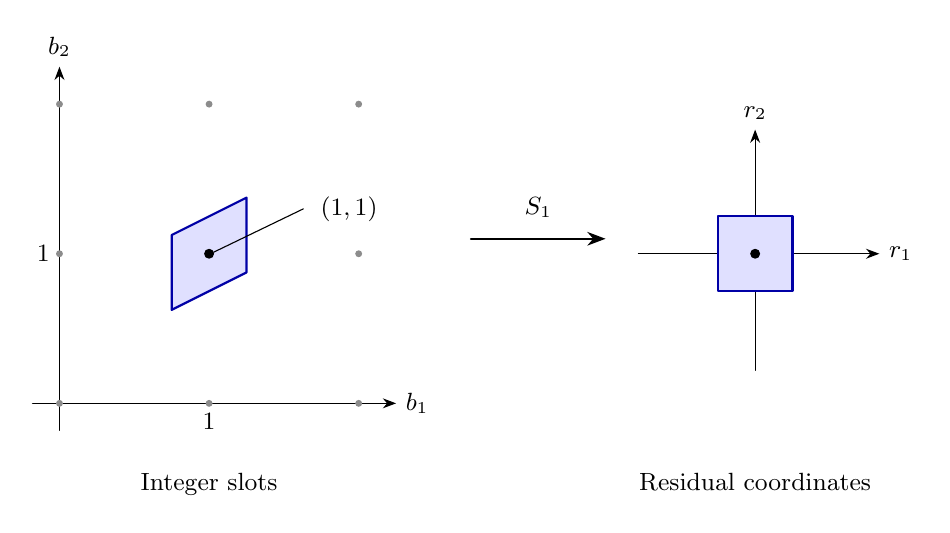
\begin{tikzpicture}[x=1.9cm,y=1.9cm,>=Stealth,
  every node/.style={font=\small},line cap=round,line join=round]
  \draw[->] (-.18,0)--(2.25,0) node[right] {$b_1$};
  \draw[->] (0,-.18)--(0,2.25) node[above] {$b_2$};
  \foreach \i in {0,1,2} {\foreach \j in {0,1,2} {
    \fill[black!45] (\i,\j) circle (1.25pt);
  }}
  \draw[blue!65!black,fill=blue!12,thick]
    (.75,.625)--(1.25,.875)--(1.25,1.375)--(.75,1.125)--cycle;
  \fill[black] (1,1) circle (1.8pt);
  \draw[thin] (1.03,1.01)--(1.63,1.30);
  \node[anchor=west] at (1.68,1.30) {$(1,1)$};
  \node[below] at (1,0) {$1$};
  \node[left] at (0,1) {$1$};
  \node[below] at (1,-.40) {Integer slots};

  \draw[->,thick] (2.75,1.1)--(3.65,1.1)
    node[midway,above=4pt] {$S_1$};

  \begin{scope}[shift={(4.65,1)}]
    \draw[->] (-.78,0)--(.83,0) node[right] {$r_1$};
    \draw[->] (0,-.78)--(0,.83) node[above] {$r_2$};
    \draw[blue!65!black,fill=blue!12,thick]
      (-.25,-.25) rectangle (.25,.25);
    \fill[black] (0,0) circle (1.8pt);
    \node[below] at (0,-1.40) {Residual coordinates};
  \end{scope}
\end{tikzpicture}
\caption{A degree-two patch of rank two, with slot weights $1,2$, at $u=1$.
Here $A_1(u)=u$, $A_2(u,b_1)=(u^2+ub_1)/2$, and
$S_1(b_1,b_2)=(b_1-1,b_2-(1+b_1)/2)$.
The shaded parallelogram is the inverse image of
$[-1/4,1/4]^2$, the permitted support of the kernel.
Only the integer pair $(1,1)$ lies in it.
For a general patch, at most one integer tuple satisfies the support
constraints, by successive determination of the slots.}
\label{fig:patch-coordinates}
\end{figure}


\subsection{The absolute starting rule}

Positive progression counting first gives an increment on boxes of a
fixed dimension. Relative lifting transfers that rule to arbitrary
dimension while keeping the number of new slots separate from the
other complexity costs. The following form is used at the terminal
boxes of the cell argument.

\begin{lemma}[Dimension-independent fresh rank]\label{ap:absolute}
There are $\xi>0$ and $C=C_k$ with the following property.
Let $p\ge2$, and let $f$ be a progression-free $[0,1]$-valued
function of mean at least $a\ge e^{-p}$ on a box of positive
dimension $n$. Suppose every side is sufficiently large, with
a sufficient logarithmic cutoff polynomial in $2+p+n$. Then,
unless the hypotheses are impossible, $f$ admits a degree-$s$
polynomial patch on a slice with positive score at target $(1+\xi)a$. The number of slots is at most
$d_0=(2+p)^C$, independent of $n$. The logarithms of inverse score,
Lipschitz norm, slice cost, and sufficient side cutoff are
polynomial in $2+p+n$.
\end{lemma}

\begin{proof}
Fix the base dimension $n_0(s)$ and prime-side comparability
constant in Proposition~\ref{counting:relative-target}.
Proposition~\ref{counting:absolute}, Lemma~\ref{counting:conversion},
and Theorem~\ref{shift:required} give an absolute rule on these
fixed-dimensional boxes, with gain $1+\xi_0$ and rank
$(2+p)^{C_k}$. The side cutoff absorbs all three requirements;
the prime sides can be odd.

Choose a small fixed $c>0$. At any actual mean
$\alpha\ge(1-c)a$, the absolute rule has logarithmic budget
$O(1+p)$ and gives positive score at the universal smaller target
$\Lambda=(1+\xi_0)(1-c)a$. If $\Lambda\ge1$, its nonnegative
test gives an impossibility rule instead. In the relative theorem
use the constant old test $1$, of rank zero, at threshold
$(1-c)a$. Its old score is at least $ca$.
Enlarge the resource parameter to a polynomial in $p+n$ to cover
the dimension, absolute cutoff, and $\log(1/(ca))$.
Theorem~\ref{lifting:relative-theorem} proves
Proposition~\ref{counting:relative-target}, including its separate
impossibility clause. Its rank conclusion is $d+d_0$, so the
enlarged resource parameter does not enlarge the fresh rank $d_0$.
Choose its fixed target discount $\epsilon_0$ and then $c$ so that
$(1-\epsilon_0)(1+\xi_0)(1-c)>1+\xi$ for a fixed $\xi>0$.
This gives the claimed rule and all its quantitative bounds.
\end{proof}

\subsection{Scalar rank and scale conventions}\label{ap:scalar-conventions}

Preparation tests the homogeneous parts of the determining polynomials.
For a box with side lengths $H=(H_1,\ldots,H_n)$, write
$H^\nu=\prod_iH_i^{\nu_i}$. A homogeneous scalar or vector
polynomial is \emph{slow} at budget $p$ if its coefficient of
$u^\nu$ has magnitude at most $\mathcal B(p)H^{-\nu}$.
It is \emph{rational} if its coefficients have a common denominator
at most $\mathcal B(p)$, with no numerator bound. The homogeneous
part at the assigned degree or weight is called its \emph{symbol}.
A polynomial is \emph{fully slow} when the same coefficient bounds
hold at every degree, including the constant coefficient, after the
box has been translated to the origin. Thus real estimates use
normalized variables, while denominator estimates use the raw
integer variables. Group-valued symbols are introduced with the
ascent representation in Section~\ref{ap:ascent}.

\subsubsection{Formal rank}\label{ap:rank-conventions}
Suppose a degree-$j$ polynomial $C_j$ takes values in a rational
space $W_j\subseteq\R^{d_j}$ on a box of sides $H$.
It has rank at least $R$ at this scale if every integer row
$\lambda\in\Z^{d_j}$ with $\|\lambda\|\le R$ and
$\lambda|_{W_j}\ne0$ has the following property: the degree-$j$
homogeneous part of $\lambda C_j$ cannot be written as a polynomial
whose coefficient of $u^\nu$ is bounded by $R/H^\nu$ plus a
rational polynomial with common denominator at most $R$.
For a system, this condition is imposed at every layer.
This is the rank condition of Definition~\ref{sampling:rank};
it is different from the slot count called the rank of a patch.

\subsection{Descending precision budgets}

\begin{definition}[Descending budgets]\label{ap:budgets}
At layer $j$, the \emph{warm data} consist of $p$, forecasts for all
dimensions and structural variable counts, gap parameters depending
only on these data, and the widths and numerical budgets already
chosen at layers strictly above $j$. A warm logarithmic bound is
polynomial in these data and does not use any $Q_i$ with $i\le j$.

The \emph{cold preliminary data} may additionally use the current
width log $Q_j$, including its forecast preparation losses, but not
the eventual rank threshold, long path scale, height of the prepared
value space, or parent-side cutoff at layer $j$. The \emph{late data}
are the perturbation, range, rank, and side choices made after all
preliminary modeling and algebraic requirements at that layer.
Their logarithms are polynomial in the cold preliminary budget.
\end{definition}

The descending choice order is opposite to the order in which paths
are sampled through the layers. Auxiliary models may have cold
complexity. Their eventual return to the original variables must
nevertheless have a warm \emph{relative width loss}; the extraction
argument preserves the defining polynomial maps exactly.
Figure~\ref{ap:budget-figure} displays the permitted dependence.

\begin{figure}[t]
\centering
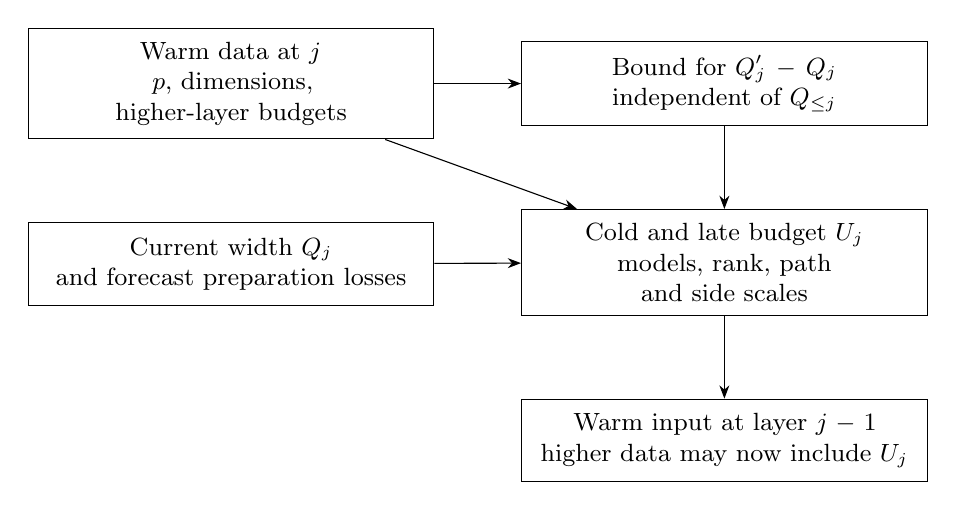
\begin{tikzpicture}[
 >=Stealth,
 box/.style={draw,align=center,text width=4.8cm,minimum height=1.05cm,
             inner sep=5pt,font=\small},
 every edge/.style={draw,->},node distance=1.05cm and 1.1cm]
\node[box] (warm) {Warm data at $j$\\$p$, dimensions, higher-layer budgets};
\node[box,right=of warm] (loss) {Bound for $Q'_j-Q_j$\\independent of $Q_{\le j}$};
\node[box,below=of warm] (own) {Current width $Q_j$\\and forecast preparation losses};
\node[box,below=of loss] (cold) {Cold and late budget $U_j$\\models, rank, path and side scales};
\node[box,below=of cold] (next) {Warm input at layer $j-1$\\higher data may now include $U_j$};
\path (warm) edge (loss)
      (warm) edge (cold)
      (own) edge (cold)
      (loss) edge (cold)
      (cold) edge (next);
\end{tikzpicture}
\caption{The allowed dependence is triangular. There is no arrow from
the current width or its cold outputs back to its relative width loss.
The full dependency schedule is proved in Section~\ref{ap:iteration}.}
\label{ap:budget-figure}
\end{figure}

\subsection{From a cell to the next certificate}

Preparation removes low-rank relations while preserving the
certificate (Proposition~\ref{ap:major:preparation}). Constrained
paths then carry it to terminal boxes
(Proposition~\ref{ap:scalar:forward}), where
Lemma~\ref{ap:absolute} supplies a quantitative score. The passive
and active return arguments carry that score back through the layers
(Proposition~\ref{ap:passive:replacement} and
Theorem~\ref{ap:active:replacement}). Extraction turns the returned
score into a triangular cell
(Proposition~\ref{ap:macro:extraction}). Finally,
Section~\ref{ap:iteration} verifies the dimension and width bounds
and iterates the increment.

\begin{figure}[htbp]
\centering
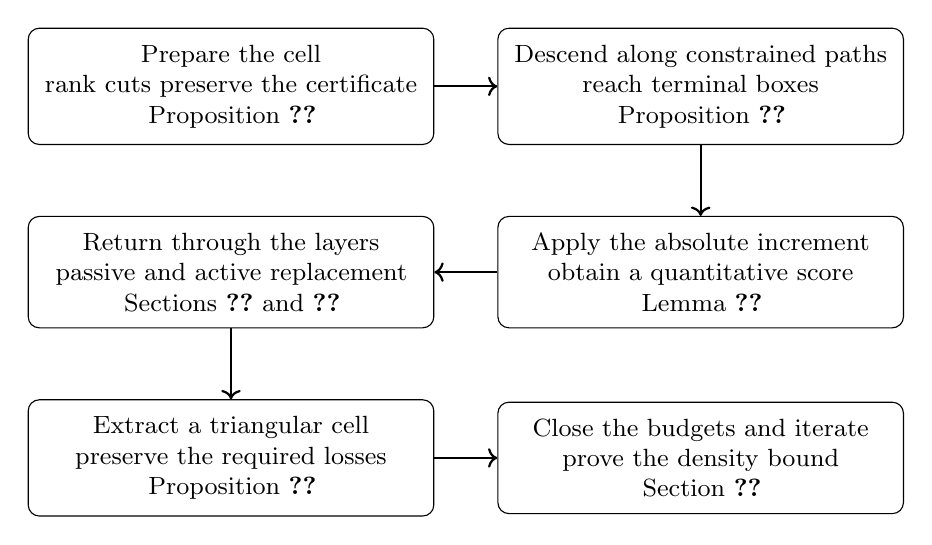
\begin{tikzpicture}[
  box/.style={draw,rounded corners,align=center,text width=0.39\linewidth,
              inner sep=6pt,font=\small},
  flow/.style={->,thick},node distance=9mm and 8mm]
\node[box] (prepare) {Prepare the cell\\
  rank cuts preserve the certificate\\
  Proposition~\ref{ap:major:preparation}};
\node[box,right=of prepare] (descend) {Descend along constrained paths\\
  reach terminal boxes\\
  Proposition~\ref{ap:scalar:forward}};
\node[box,below=of descend] (absolute) {Apply the absolute increment\\
  obtain a quantitative score\\
  Lemma~\ref{ap:absolute}};
\node[box,left=of absolute] (return) {Return through the layers\\
  passive and active replacement\\
  Sections~\ref{ap:ascent} and~\ref{ap:active}};
\node[box,below=of return] (extract) {Extract a triangular cell\\
  preserve the required losses\\
  Proposition~\ref{ap:macro:extraction}};
\node[box,right=of extract] (iterate) {Close the budgets and iterate\\
  prove the density bound\\
  Section~\ref{ap:iteration}};
\draw[flow] (prepare) -- (descend);
\draw[flow] (descend) -- (absolute);
\draw[flow] (absolute) -- (return);
\draw[flow] (return) -- (extract);
\draw[flow] (extract) -- (iterate);
\end{tikzpicture}
\caption{The main proof route.  Preparation and extraction preserve the
triangular dependence of the width losses; the absolute increment
controls the number of fresh determining coordinates.}
\label{ap:proof-route}
\end{figure}


During preparation the polynomial $C_j$ takes values exactly in a
rational subspace $W_j\subseteq E_j=\R^{d_j}$, initially the full
space. The rank test defined above and in Definition~\ref{sampling:rank}
requires that no integer
row of norm at most $R_j$, nonzero on $W_j$, has a degree-$j$
symbol that is slow plus rational at that threshold. The test is made
on the current path box at a history that has survived the earlier
tests. The histories arriving at each layer carry the subprobability
law of Section~\ref{ap:path:stopped-tree}; stopping removes mass
without renormalizing the survivors.
Its failure probability may charge $Q_{\ge j}$ but not lower
widths. There is no single root equidistribution test at the finest
precision of all layers.

At a successful layer use a Haar center in
$W_j/(W_j\cap\Z^{d_j})$, conditioned to the feasible range
specified in Section~\ref{ap:path:stopped-tree}. The lift has exact identity
\[
                     C_j-c=y+\beta,
\]
where $y\in\R^{d_j}$ is the small real residual and
$\beta\in\Z^{d_j}$ is the integer lift. The raw determining
slot is $b_j=\beta+b_{j,0}$ for a constant
integer vector. This convention matters: every later old polynomial
uses the actual integer slot, not an approximation to its value.
Structural numbers of path columns are fixed polynomials of the
input dimensions before any numerical precision is chosen.
Consequently all ambient dimensions along a branch are polynomial
in the current dimension forecasts. Sides are selected to support
the next layer and finally Lemma~\ref{ap:absolute}.

The return processes layers from $D$ down to $1$. Layers $j>s$
are passive: the new patch does not acquire their integer arguments.
At the final $s$ active layers its weights may increase by fixed
factors, while the old determining equations and their weights stay
exact. This distinction is why a fixed $D$ can be chosen before the
iteration, even though the number of slots grows.

The input certificate and the returned score carry different information.
Preparation needs only
the strict inequality in the input certificate: its selections do not charge
the inverse of that inequality's excess. Proposition~\ref{ap:scalar:forward}
then gives terminal means near the current threshold on a quantitatively
large set of paths. Lemma~\ref{ap:absolute} supplies the quantitative score
needed for ascent. Thus all subsequent approximation accuracies can be
chosen from the recorded budgets, independently of the original excess.

The analytic proofs are grouped separately.
Table~\ref{ap:interface-table}, at the entrance to that part,
locates each input statement and its proof.

\section{Constrained paths and their detection estimates}\label{ap:paths}

At one layer of a triangular cell, we seek many integer-affine maps
$\psi(t)=x+Vt$ along which the current polynomial has a small
polynomial residual and an exact integer-polynomial lift. The affine
maps preserve arithmetic progressions; the polynomial identity will
preserve the determining equations when a new patch is returned to
the parent. We construct their probability law in this section.

There are two comparison estimates to prove for that law. With the
center fixed, tests chosen separately on the sampled boxes must be
detectable on the parent. After averaging the center, the one-site
distribution must approximate the parent distribution. Below the
current degree, the first comparison must be measured relative to
the small chart: charging its reciprocal mass to the output
complexity would charge the current width to its own relative loss.

The coefficient density will be a product law on an abstract
coefficient torus. The actual ensemble is the integer spatial law
weighted by that density. These are different probability spaces.
The construction below defines both; high rank will supply the
comparison between them. The general estimates for coefficient
modes and polynomial images are proved in
Appendices~\ref{sampling:constrained-section} and~\ref{cube:section}.

Throughout this section, $j$ is the current layer, $d=d_j$,
$W\subseteq\R^d$ is rational, and
\[
 U=\prod_{a=1}^n\{0,\ldots,H_a-1\},\qquad
 C: \R^n\longrightarrow W,\qquad \deg C\le j.
\]
Lower layers have already been substituted.  Rank means the ordinary
rank condition of Definition~\ref{sampling:rank}, with the single tag
$j$: no integer row of norm at most $R_j$, nonzero on $W$, takes the
degree-$j$ symbol of $C$ to a slow-plus-rational polynomial at bound
$R_j$.  Warm, cold-pre, and late choices have the meanings fixed in
Definition~\ref{ap:budgets}.  All degrees and cube orders below belong to a
fixed finite range.  Structural numbers of columns are polynomial in
dimensions and are fixed before numerical precisions.

\subsection{Normalized lift charts}

Put $\Lambda=W\cap\Z^d$ and
$\Lambda'=\operatorname{proj}_{W^\perp}\Z^d$.
Choose the basis $v_i$, $1\le i\le\dim W^\perp$, of the projected
lattice $\Lambda'$ supplied by Lemma~\ref{sampling:lattice-chart},
and set
\begin{equation}\label{ap:path:mass}
 K_i=\max(1,\lceil |v_i|^{-1}\rceil),\qquad
 k_i=\max(1,\lceil K_i v\rceil),
 \qquad
 m_j=v^{\dim W}\frac{\prod_i k_i}{\covol(\Lambda)}.
\end{equation}
Here $v$ is a sufficiently small warm fraction of $w_j$.  All lift
coordinates use this same physical width.  More precisely, $v/w_j$ has
logarithmic cost polynomial in dimensions and $\log\gamma^{-1}$.
Principal amplitudes in normalized lift units, and the proportionality
constants in inactive side lengths, can have logarithmic costs depending
only on dimensions.  They are chosen small enough that all true and
ideal lifts lie well inside a buffered chart of radius comparable to
$v$, itself inside the required gap.  These charts are narrow enough
that every Boolean difference of an order used below has components
of magnitude less than $1/2$.

For a center $c\in W/\Lambda$, choose a representative in $W$.  On a
uniqueness chart write
\[
 C(u)-c=y(u)+\beta(u),\qquad \beta(u)\in\Z^d.
\]
The sheet coordinates satisfy
\[
 \operatorname{proj}_{W^\perp}y=\sum_i v_i z_i
       =-\operatorname{proj}_{W^\perp}\beta.
\]
Choose integer lifts of the basis vectors $v_i$, and let $l(z)$
be their integer linear combination. Then $\beta+l(z)\in\Lambda$.
Choose an integer basis of $\Lambda$ and let $w$ be the coordinates
of $\beta+l(z)$ in that basis. Primitivity of $\Lambda$ shows that
$\beta\mapsto(z,w)$ is an integer unimodular change of coordinates.
Here $w$ is a deck coordinate, not a width. A residue character of
$(z,w)$ is therefore a residue character of $\beta$ at the same
modulus; the real size of the basis coefficients does not enter
this assertion.

\begin{lemma}[Chart mass and normalized coordinates]\label{ap:path:chart}
The quantities $m_j$ and $m_j^{-1}$ have cold-pre bounds independent of
the height of $W$.  On a buffered chart the coordinates
$y_W/v$ and $z_i/k_i$ have dimension-controlled norms in terms of $y/v$.
The row defining $z_i$ on the ambient lift has norm at most
$\exp(\operatorname{poly}(d))K_i$, is integral on $\Z^d$, and
annihilates $W$.

A bounded warm enlargement of the chart has Haar measure at most a
warm multiple of $m_j$.  A ball of a warm fraction of radius $v$,
centered at a feasible torus point and with the prescribed room, has
Haar measure at least a warm inverse multiple of $m_j$.  These relative
bounds do not depend on any width when the radius ratios use only
dimensions and $\gamma$.
\end{lemma}

\begin{proof}
Lemma~\ref{sampling:lattice-chart} gives
\[
 \covol(\Lambda)\asymp_{\exp(\operatorname{poly}(d))}\prod_iK_i
\]
and dimension-controlled maps between the projected Euclidean
coordinates and $z_i/K_i$.  Since
$k_i\asymp\max(1,K_i v)$, multiplying the latter coordinates by
$K_i v/k_i\le1$ proves the asserted upper norm bound.  The dual
projected lattice is the integral annihilator of $W$, giving the
integral rows and their stated norms.  If $q=\dim W^\perp$, then
\[
 \exp(-\operatorname{poly}(d))v^d
       \le m_j\le \exp(\operatorname{poly}(d))v^{\dim W}.
\]
In particular its logarithmic costs involve $\log v^{-1}$ but not
subspace height.

Haar measure in these coordinates is Lebesgue measure on $W$ times
counting measure on the sheets, divided by $\covol(\Lambda)$.
Counting sheet coordinates in a dimension-controlled parallelepiped
and integrating on $W$ gives the upper bound.  Around a feasible
sheet, a smaller such parallelepiped contains at least a
dimension-controlled multiple of $\prod_i\max(1,\tau k_i)$ sheet
points when its radius is $\tau v$; this is at least
$\tau^q\prod_i k_i$ up to dimension factors.  Integration on $W$
supplies the other $\tau^{\dim W}$ factor.  This proves the lower
bound, including arbitrary fixed real translations of the chart.
Feasibility is necessary: no assertion is made that an arbitrary
translated small box meets the torus.
\end{proof}

\subsection{The coefficient law and the actual path ensemble}

First consider the model $W=\R^d$, where there are no discrete
sheet coordinates. We want the spatial directions and the small-lift
directions to be recoverable separately. The reference lift law
therefore uses disjoint blocks of $j$ parameters with a common
side $L$, to be selected later. On a lift axis $a$, its principal
part has the form
\[
 \frac{y_a^{\rm ideal}(t)}v=\eta_a+
       \sum_B c_{aB}\prod_{\ell\in B}\frac{t_\ell}{L},
\]
with the normalized $c_{aB}$ bounded away from zero. The constant
$\eta_a$ supplies the local translation. The blocks for different
axes are disjoint, and a separate kernel block controls the spatial
image. Fixing all but one variable in each selected product at
normalized values bounded away from zero gives independent
directions in this ideal model. Repeating the products
on further disjoint blocks also smooths their one-site and cube
evaluation laws.

The reason to recover lift directions rather than raw integer
coefficients comes from the lift identity we require. We will
arrange that $C(\psi(t))-c=y(t)+\beta(t)$ is a polynomial identity
of degree at most $j$. Its top homogeneous parts then give
\[
 \beta_{[j]}(t)-C_{[j]}(\psi_{[1]}(t))=-y_{[j]}(t).
\]
Here brackets denote ordinary homogeneous degree. Thus the products control the deviation of the integer variable
from its prescribed polynomial value without any bound on the
coefficients of $C$. Small remaining lift coefficients and small
nonkernel spatial displacements perturb this ideal recovery map;
they do not give exact independence to the full map.

For a rational $W$, the projected lift coordinates are integer
sheets. Their available ranges determine whether the preceding
products can use long parameters or must instead use coefficient
one and shorter parameters. We now prescribe those ranges and
the additional columns needed for residue tests and exact sheet
translations. All independence in this prescription belongs to
the reference coefficient law and the separate spatial law.
The actual path law couples them by the tilt below.

After the pre requirements are fixed, choose a perturbation
parameter $0<\sigma<1$ and a range parameter $A\ge2$, in that
order. Rank thresholds and parent sides will be chosen later.
Choose a scale gap with no $k_i^{1/j}$ between $L$ and $AL$.
For example, among more than $\dim W^\perp$ consecutive disjoint
multiplicative intervals of ratio $A$, at least one contains none
of these numbers. Hence this choice is possible with
$A\le L\le A^{O(1+d)}$.  With a fixed sufficiently large
degree-dependent $C_*$, call a sheet axis
\[
 \begin{array}{ll}
 \text{inactive}& k_i\le L^j,\\
 \text{moderate}& (AL)^j\le k_i\le L^{C_*},\\
 \text{enormous}& k_i>L^{C_*}.
 \end{array}
\]
There are only polynomially many numbers to avoid, so $\log L$ can
be chosen with the permitted late bound without using their magnitudes.
Rounding is performed with fixed buffers at the cutoffs.
An active sheet axis means a moderate or enormous axis.

The parameter box is
$\mathcal T=\prod_\ell\{0,\ldots,T_\ell-1\}$.
We prescribe its columns, the independent reference law of the
lift coefficients, and the supports of the separate spatial law
as follows. The actual coefficients of $C(x+Vt)$ are determined
by $(x,V)$; the tilt defined below combines these two laws.
\begin{enumerate}
\item To keep the spatial image nondegenerate independently of the
principal lift directions, spatial kernel columns have side $L$.
In normalized spatial coordinates their matrices lie in buffered neighborhoods of fixed
invertible matrices, at a common warm spatial scale.  The inverse
norms are warm-bounded throughout the supports.
\item Continuous and active lift axes have independent dedicated
blocks of $j$ columns, all of side $L$.  Their principal monomials
are squarefree products on disjoint blocks.  In normalized units
$y_W/v$ and $z_i/k_i$, the principal amplitudes have buffered
supports bounded away from zero at the chosen dimension scale.
Equivalently, a principal raw coefficient has size comparable to
$v/L^j$ on a continuous axis and $k_i/L^j$ on an active sheet
axis, with the corresponding smooth continuous or integer law.
\item On an inactive axis, integral coefficients cannot be made
arbitrarily small. We therefore keep the product coefficient
exactly one and shorten the dedicated sides to quantities comparable
to $k_i^{1/j}$ at the prescribed dimension factors.  If these sides would be below a specified
warm minimum, omit the axis: set \emph{every} coefficient, including
the constant, equal to zero, and supply no columns for it.  Hence
omitted $k_i$ are warm-bounded.  Otherwise supply one additional
nonkernel column $t_{i,0}$, with side comparable to $k_i$.
Its coefficient is one so that translating it translates the
sheet output by exactly the same amount, as needed for the
later affine sections. Set
\begin{equation}\label{ap:path:inactive-polynomial}
 z_i(t)=z_i(0)+t_{i,0}
                 +\sum_{\text{dedicated blocks }B}\prod_{\ell\in B}t_\ell.
\end{equation}
There are no other terms on this axis.  The common proportionality
constants are small enough for chart containment.
\item To test congruence relations without sharing the principal
smoothing variables, add a structural polynomial number of free
nonkernel columns, of side $L$, disjoint from the preceding blocks.
Their independent leading coefficient data supply the
residue-test vectors in the reference comparison law.  On moderate
axes, put independent small perturbations on all pure-free
nonconstant monomials, with integer coefficient widths comparable to
$k_i\sigma/T^\nu$.  Other nondesignated moderate coefficients remain
zero. The scale gap makes the selected integer ranges broad
enough for later individual-modulus tests. On continuous and
enormous axes, each remaining nonconstant
monomial $t^\nu$ has an independent small coefficient whose width
in the normalized output coordinates is comparable to
$\sigma/T^\nu$. The continuous coefficients have smooth laws.
The enormous-axis coefficients are integers, with the smooth
discrete laws specified below.
\end{enumerate}
Here and below fixed structural factors may multiply these widths.
Every constant lift coefficient has an independent law of fixed
warm support in its normalized units. When its integer range is
too short for that law it is fixed at zero; its corresponding
$k_i$ is then warm-bounded. Counts of kernel and product blocks
are fixed polynomials in the structural dimensions, large enough
for the fixed cube orders and smoothing orders used below, with
spare blocks for smoothing. Numerical precisions never increase
these counts. Every nonomitted side exceeds the specified warm
minimum, which may include higher-layer parent and separation
requirements. Every side is $O(L^j)$.

We specify the coefficient laws as well as their supports.
Fix a nonnegative, nonzero smooth bump $\varphi$ supported in
$(-1,1)$ and positive on a neighborhood of zero.
An integer coefficient with center $a$ and scale $S$ has law
\[
 \Pr(\alpha=k)=
 \frac{\varphi((k-a)/S)}
      {\sum_{r\in\Z}\varphi((r-a)/S)}.
\]
The center and scale place this support strictly inside the
prescribed interval and ensure that its positive region contains
an integer, so the denominator is positive. Coefficients fixed at zero or one have their
stated point-mass laws. Continuous coefficients are their centers
plus their prescribed widths times independent variables with
fixed smooth buffered densities. All these choices are independent
across coefficient positions and output axes.

For a monomial $t^\nu$, let $f_\nu$ be the resulting density of its
coefficient in the orthogonal $W$ coordinates, and let
$p_{i,\nu}$ be the probability mass of its coefficient on sheet
axis $i$. On the coefficient torus $W/\Lambda$, the local Haar
measure is $du_W\,d\#z/\covol(\Lambda)$. Consequently
\[
 \covol(\Lambda)\,f_\nu(u_W)\prod_i p_{i,\nu}(z_i)
\]
is the density of this coefficient law relative to Haar.
The selected supports lie in a buffered coefficient chart.
Their product over $|\nu|\le j$ defines a probability density
$\mathcal D_c$ on
$\prod_{|\nu|\le j}W/\Lambda$; the center $c$ shifts only the
constant coefficient. In particular $\int\mathcal D_c=1$.

We also choose a law $\rho(x,V)$ on integer spatial coefficients.
The root $x$ is nearly uniform on a buffered interior box, with
a smooth transition near its boundary. In each spatial kernel
block the normalized matrix lies in a product neighborhood of a
fixed invertible matrix at the selected warm spatial scale.
Its integer entries are sampled independently by smooth buffered
bumps in their normalized intervals, with the same normalization
as the integer coefficient law above. Every nonkernel entry is
independent and has a smooth profile
supported in
\[
             |V_{a\ell}|
             \le \frac{c_0\sigma H_a}{mT_\ell},
\]
where $m$ is the number of columns and $c_0>0$ is a fixed small
constant. These widths become long integer intervals when the
parent sides are chosen. Their total normalized displacement
is $O(\sigma)$. All supports have enough room that every path
lies in $U$.

The actual law of the affine maps is
\begin{equation}\label{ap:path:tilt}
 d\mathbb P_c(\psi)
  =\frac{\rho(x,V)\mathcal D_c(\operatorname{coeff}C(x+Vt))}
  {Z_c},\qquad \psi(t)=x+Vt.
\end{equation}
The normalizer in this formula is
$Z_c=\E_\rho\mathcal D_c(\operatorname{coeff}C(x+Vt))$.
The identity $\int\mathcal D_c=1$ concerns abstract Haar coefficients;
the conclusion $Z_c=1+o(1)$ will use high rank of the actual
polynomial coefficients.

There is a second distinction when residue information is needed.
On the finite cover $W/M\Lambda$, Haar measure above a coefficient
in $W/\Lambda$ is uniform on its $M^{\dim W}$ deck choices.
Thus the deck coefficients modulo $M$ are independent uniform
variables conditional on the small-lift coefficient data under
this comparison law. The actual integer spatial law will only
approximate the resulting joint residue law at each prescribed
individual modulus. It need not have this exact conditional
independence after real coefficient values are fixed.

By contrast, the lift identity on a path is exact. On the support
of $\mathcal D_c$, subtracting the small real coefficient lifts
from $C(x+Vt)-c$ leaves integer monomial coefficients. Their sum
is a polynomial $\beta(t)$, and the small coefficients sum to
$y(t)$. Chart containment identifies these polynomials with the
site lifts throughout the path.

We will use high rank through the following Fourier estimate.
Consider coefficient characters on a prescribed integer cover,
represented by rational ambient rows $\lambda_\nu$ whose
denominators divide its modulus. For fixed parameter sites
$t_\omega$, evaluation sends a
$W$-valued polynomial coefficient array $(a_\nu)_\nu$ to
$(\sum_\nu a_\nu t_\omega^\nu)_\omega$. A coefficient mode
$e(\sum_\nu\lambda_\nu a_\nu)$ \emph{factors through these sites}
if its real linear functional is a linear combination of the
evaluation functionals; equivalently, it vanishes on their
common kernel. Here $e(z)=\exp(2\pi i z)$.

For one site, or sites
$t_\omega=t_0+\sum_{i=1}^q\omega_it_i$ forming an affine Boolean
cube of fixed order with independent differences, Lemma~\ref{sampling:analytic-removal}
removes every mode which does not factor through the sites:
\[
 \left|\E_\rho
 e\!\left(\sum_\nu\lambda_\nu
          \operatorname{coeff}_\nu(C(x+Vt))\right)
       \prod_\omega F_\omega(x+Vt_\omega)\right|
 \le\varepsilon
 \qquad(|F_\omega|\le1).
\]
The rank and parent-side thresholds depend polynomially in
logarithmic scale on the prescribed Fourier frequencies and
coefficient mass, cover modulus, spatial smoothness, inverse
error, $\log L$, and $\log\sigma^{-1}$. They do not depend on the
height of $W$. Spatial residue conditions may be included.
With no site insertions, every nontrivial coefficient character
is removed. The estimate applies to the Fourier expansion of
$\mathcal D_c$ before dividing by $Z_c$.

Factoring through real evaluation need not give a character on
the original evaluation torus. Clearing the denominators of a
rational right inverse gives a finite cover on which it does.
The cube comparison below retains this cover. For a single site
the constant coefficient already gives an integral right inverse.
These observations specify the estimate used in the following
lemma; its proof remains in the appendix.

\begin{lemma}[The normalized one-layer ensemble]\label{ap:path:ensemble}
For the law just defined, sufficiently large permitted rank and parent
side cutoffs give the following conclusions, uniformly in the center.
\begin{enumerate}
\item $Z_c=1+o(1)$, and on every retained path
\begin{equation}\label{ap:path:exact-lift}
 C(\psi(t))-c=y(\psi(t))+\beta(\psi(t))
\end{equation}
is a polynomial identity.  The small lift is fully slow at width $v$;
$\beta\circ\psi$ has integral monomial coefficients.
\item The non-site-mode removal of
Lemma~\ref{sampling:analytic-removal}, and the Haar and individual-cover
conclusions of Corollaries~\ref{sampling:normalization}
and~\ref{sampling:finite-residues}, hold with cold-pre requests and
late errors.  In particular, on each prescribed individual modulus,
the relevant coefficient residues have the product chart/deck law,
independently of the unweighted spatial residues, to arbitrarily small
prescribed total variation.  On moderate axes the pure-free
nonconstant coefficients are independently uniform to this accuracy
once the range parameter is chosen sufficiently large.
\item Noninjective paths can be discarded at any prescribed cold-pre
probability.  At fixed center the averaged one-site law is supported
on the buffered chart and has density at most $B/m_j$ relative to
uniform measure on $U$, apart from arbitrarily small excess mass,
where $B$ is warm-bounded.
\item Given a warm spatial error $\epsilon>0$, the root law can be
chosen so that Haar mixing of centers gives the one-site upper bound
$(1+\epsilon)$ times the uniform law, and the corresponding lower
bound $(1-\epsilon)$ away from a warm-thickness boundary strip,
each with arbitrarily small cold-pre additive error against every
nonnegative function bounded by one.  The spatial scale and strip
thickness do not depend on $Q_j$.
\end{enumerate}
\end{lemma}

\begin{proof}
The independent coefficient density has Haar integral one.  On its
support subtracting the specified small coefficient lifts leaves
integral coefficients.  Summing the resulting monomials proves
Equation~\eqref{ap:path:exact-lift}; uniqueness of the chart identifies
this polynomial lift with the site lift throughout the path.

We check the quantitative hypotheses for Fourier removal rather than
deduce $Z_c=1$ from the abstract normalization.  In a coefficient
chart the Haar density has the factor
$\covol(\Lambda)/(v^{\dim W}\prod_i k_i)=m_j^{-1}$.
The remaining factors are normalized continuous densities and
normalized discrete bumps.  On axes with $k_i\le L^{C_*}$, singleton
interpolation costs only $O(\log L)$ in addition to cold-pre costs.
This includes omitted axes.  On enormous axes all coefficient ranges
contain many grid points.  Since $T^\nu\le L^{j^2}$ for degrees at
most $j$, their normalized smooth interpolation has logarithmic costs
polynomial in the cold-pre budget, $\log\sigma^{-1}$, and $\log L$,
when $C_*$ is sufficiently large.  Lemma~\ref{ap:path:chart} controls
all normalized coordinate maps independently of orientation and
height.  Buffered ambient chart extensions can therefore be
periodized and Fourier approximated with just these costs.

On a modulus cover multiply by the residue character of the chart
index $\beta$.  Rows defining $(z,w)$ reduce modulo that modulus,
so no real deck-basis norm is needed.  The same ambient extension
works on the cover with its individual logarithmic modulus cost.
The displacement proof of Lemma~\ref{sampling:analytic-removal}
only changes by replacing its parameter bound $L$ with $O(L^j)$.
Its translating boxes and the parent cutoff still have permitted
late logarithmic costs.  Thus it removes each non-site mode with
arbitrary bounded site insertions.  With no insertions it removes
every nontrivial coefficient mode; the trivial mode is the Haar
integral one.  This proves $Z_c=1+o(1)$.  Translating $c$ changes
Fourier phases but none of the bounds, proving uniformity.

For each prescribed residue vector apply this argument on its own
cover and sum per-atom errors.  The logarithm of the atom count is
polynomial in dimensions and the individual modulus log.  This is
the total-variation argument of
Corollary~\ref{sampling:finite-residues}, with the ambient extension
just verified.  A moderate pure-free coefficient of top degree has
width at least a structural factor times $A^j\sigma$; coefficients
of smaller degree have no smaller range.  Choosing $A$ after the
individual-modulus requests makes every such smooth integer law
uniform modulo that modulus to the required accuracy.  Parent sides
similarly make spatial free entries broad.  The deck laws are
uniform independently of the sheet data.  This proves the full
joint assertion, not merely a claim about designated top monomials.

The independent constant coefficient has Haar density at most
$B/m_j$ for a warm $B$.  The surviving one-site weight under
non-site removal is its convolution with the probability law of
the other coefficient contributions, so has the same cap.  The
independent spatial root has a warm cap conditional on all slopes.
Removal with arbitrary site indicators consequently bounds the
excess mass above a fixed warm multiple of $m_j^{-1}$ by the
requested error.  All actual supports are buffered.

When centers are mixed, a mode factoring through one site has its
site row as its constant coefficient row.  Center integration kills
every nontrivial such row; removal kills the nonfactoring modes.
Only the unweighted spatial law remains.  Choose its root nearly
uniform on an interior box and make all spatial displacements a
smaller warm fraction of the sides.  Its translate has the asserted
upper density everywhere and lower density off the indicated strip.
Only the Fourier removal error, not that strip, is requested at
cold precision.

Finally, for a fixed nonzero difference $a=t-t'$, the equation
$Va=0$ determines at most one value of an entry in a column for
which $a_\ell\ne0$.  Smooth broad spatial laws, a union bound over
at most $O(L^{2jm})$ pairs, and the permitted late supremum bound
of the tilt make collisions negligible by increasing parent sides.
This completes all the claims in the permitted choice order.
\end{proof}

\subsection{Comparing sampled and ambient tests}

\subsubsection{Niltests}\label{ap:niltest-conventions}
A rational filtered nilmanifold of degree $q$ consists of a connected,
simply connected nilpotent Lie group $G$, a cocompact lattice $\Gamma$,
and connected rational subgroups
\[
 G=G_1\supseteq\cdots\supseteq G_{q+1}=\{1\},
 \qquad [G_i,G_j]\subseteq G_{i+j}.
\]
Rationality is measured in fixed exponential coordinates on the Lie
algebra $\mathfrak g=\log G$, with rational bases for
$\mathfrak g_i=\log G_i$. A polynomial map $g:\Z^n\to G$ is
adapted when $\log g$ modulo $\mathfrak g_{i+1}$ has degree at
most $i$, using weighted degree when variable weights are assigned.
A \emph{niltest} is the function $u\mapsto F(g(u)\Gamma)$,
where $F$ is bounded and Lipschitz on $G/\Gamma$. The metric is
the quotient of the right-invariant Riemannian metric making the
chosen coordinate basis orthonormal at the identity.

Complexity at most $p$ means that $\dim G$, the logarithmic heights
of the structural constants and filtered bases, and
$\log(2+\|F\|_\infty+\Lip F)$ are at most $p$, with
\[
 l\Z^{\dim G}\subseteq\log\Gamma\subseteq l^{-1}\Z^{\dim G}
 \quad\text{for some integer }1\le l\le e^p.
\]
A metric change includes the logarithm of its comparison constant in
this budget. No coefficient bound is imposed on the orbit $g$.
On $\Z/N\Z$, evaluation uses representatives $0,\ldots,N-1$;
degree-zero tests are constants, and dimension zero is allowed.
Definition~\ref{prelim:niltest} repeats these conventions where the
rational calculus is developed. The equivalence with adapted
Taylor/binomial polynomial sequences is proved there.


\subsubsection{Cube normalization}\label{ap:cube-conventions}
For a finite integer box $Q$, let $\operatorname{Cub}_j(Q)$ be the
set of tuples $(x,h_1,\ldots,h_j)$ for which every vertex
$x+\omega\cdot h$, $\omega\in\{0,1\}^j$, belongs to $Q$.
Writing $\mathcal C z=\overline z$, we use
\[
 \|f\|_{U^j(Q)}^{2^j}
 =\frac{1}{|\operatorname{Cub}_j(Q)|}
   \sum_{(x,h)\in\operatorname{Cub}_j(Q)}
   \prod_{\omega\in\{0,1\}^j}
       \mathcal C^{|\omega|}f(x+\omega\cdot h).
\]
On a finite abelian group, all parameters instead have independent
uniform averages. In particular, the constant function $1$ has norm
one under both conventions. Formula~\eqref{prelim:box-gowers}
and the identities following it give the exact comparison with
zero extension to a product of cyclic groups and the cube-count
weights required when taking derivatives.




A \emph{normalized site twist} is a unit-bounded function localized
to a buffered chart which is a product, or a bounded-complexity
combination of products, of a smooth function of $(u/H,y/v)$ and a
bounded-modulus function of $(u,\beta)$.  Smoothness is measured in
these normalized variables.  Such a twist need not have warm
Lipschitz cost as a function on the unlocalized ambient torus.

\begin{lemma}[Cube comparison in chart units]\label{ap:path:comparison}
Fix slice costs, a fixed cube order $q$, and a requested accuracy.
For a fixed permitted parameter slice $B$, the sampled functional
\[
 (P_\omega)_\omega\longmapsto
 \E_\psi\E_{\mathbf t\in\operatorname{Cub}_q(B)}
            \prod_{\omega\in\{0,1\}^q}P_\omega(\psi(t_\omega))
\]
is, uniformly for $|P_\omega|\le1$, approximated to the requested
accuracy by
\[
 \sum_\alpha c_\alpha
 \E_{\mathbf u\in\operatorname{Cub}_q(U)}
       \prod_{\omega\in\{0,1\}^q}
                P_\omega(u_\omega)J_{\alpha,\omega}(u_\omega).
\]
The site twists $J_{\alpha,\omega}$, coefficient mass
$\sum_\alpha|c_\alpha|$, and number of terms have cold-pre bounds.  If $q\le j$ and
the request is warm, its ambient output can instead be written
\begin{equation}\label{ap:path:sparse-comparison}
 \sum_\alpha c_\alpha\,
 \E_{\text{ambient cubes}}
       \prod_{\omega\in\{0,1\}^q}
       P_\omega(u_\omega)\frac{J_{\alpha,\omega}(u_\omega)}{m_j},
\end{equation}
with warm total coefficient mass, warm normalized site twists
$J_{\alpha,\omega}$, and an arbitrarily small prescribed warm
additive error, uniformly for arbitrary $|P_\omega|\le1$.
Finite sums suffice.  Only the error transfer and removal, not the
output twists or coefficient mass, use cold or late costs.
\end{lemma}


The proof appears after the general cube comparison in
Appendix~\ref{cube:section}. Its factors depend only on individual
ambient sites. This is the feature that lets a large sampled cube
average yield an ambient niltest correlation.

Choose a nonnegative smooth cutoff $\chi$ supported in a buffered
uniqueness chart and equal to one on all path and twist supports.
For fixed center $c$, normalized chart measure on $U$ is the
probability measure
\[
 \mu_c(\{u\})=
 \frac{\chi(C(u)-c)}{\sum_{v\in U}\chi(C(v)-c)}.
\]
The denominator is positive for the sufficiently large rank and
side choices below. This measure is used only for the warm
detection assertion; the approximation seminorm is defined from
the actual path law.

Fix a degree $r$, permitted slice costs, and local test complexities.
For a site input $g:U\to\C$, put
\[
 X_r(g)=\E_{\psi\sim\mathbb P_c}
        \sup_{B,F}\left|\E_{t\in B}g(\psi(t))F(t)\right|,
\]
where $B$ ranges over the permitted slices of $\mathcal T$ and $F$
over unit-bounded local niltests of degree $r$ and the prescribed
complexity. Each path may choose its own slice and niltest. An
ambient atom is a product $J(u)N(u)$, where $J$ is a normalized
site twist and $N$ is an ordinary ambient degree-$r$ niltest;
both factors may be taken unit-bounded.

\begin{theorem}[Pathwise detection and approximation]
\label{ap:path:detection}
Prescribe finitely many testing degrees in the fixed allowed range,
local test complexities, slice costs, input caps, and accuracies.
The later parameters of the one-layer construction can be chosen
once so that the following assertions hold for this same ensemble,
uniformly in the center and the site input.

For cold-pre requests, if a cold-pre-bounded input satisfies
$X_r(g)\ge a>0$, with $\log(1/a)$ bounded by cold-pre data,
then $g$ correlates in uniform parent measure with an ambient
atom of cold-pre complexity, and the logarithm of the reciprocal
correlation has a cold-pre bound. Every $|g|\le1$ can also
be approximated in $X_r$, to the prescribed cold-pre accuracy,
by a linear combination of such atoms with cold-pre coefficient
mass and number of terms.

If $r<j$ and the requests are warm, every warm-bounded input
with $X_r(g)\ge a>0$ and a warm bound for $\log(1/a)$
correlates in $\mu_c$ with an ambient atom of warm complexity,
with a warm bound for the logarithm of the reciprocal correlation.
The atoms, coefficient mass, and number of terms in the
$X_r$ approximation also have warm bounds. These
bounds may use the omission threshold but do not use $Q_j$ or
the height of $W$.

For a specified larger input cap, include its logarithm in the
request budget and rescale. Increasing the requested accuracy,
test, or path budgets changes the corresponding warm or cold-pre
output logarithms polynomially. All path probabilities and
testing suprema refer to the law before productive paths are
selected.
\end{theorem}

\begin{proof}[Proof of the cold clause]
The ordinary argument of Lemma~\ref{cube:pathwise-detection}
applies to the ensemble above by Lemma~\ref{ap:path:comparison}.  Indeed, mesh endpoints and enumerate strides to reduce
the separately chosen slices to finitely many possibilities.  A
short side has a bounded number of points and can be enumerated
directly.  A positive fraction of detecting paths therefore has
a large $U^{r+1}$ norm on one common slice.  The niltests on these
paths need not be the same.

Lemma~\ref{ap:path:comparison} transfers their averaged cube
power to a mixed ambient cube correlation.  When all physical
chart costs are included in the cold preliminary budget, its
site factors have controlled caps.  Gowers--Cauchy--Schwarz and
Theorem~\ref{prelim:inverse}, as in the cited detection proof,
give an ambient degree-$r$ niltest times a permitted site twist
correlating with the input.  Degree zero uses the two independent
sites of a one-cube and gives a twist alone.

To pass from detection to approximation, let $m_U$ be the full
one-site density relative to uniform measure on $U$.  If every
permitted slice has at least fraction $\delta_{\rm sl}$ of the
full parameter box, then
\[
              X_r(\phi)\le
       \delta_{\rm sl}^{-1}\mathbb E_U m_U|\phi|.
\]
Lemma~\ref{ap:path:ensemble} bounds the excess mass above a cap
of cold preliminary size.  Doubling the cap bounds the mass of
the resulting tail by twice that excess.  Select this cap first,
then request the tail accuracy needed by Lemma~\ref{cube:separation}.  That
lemma produces the finite approximation, with controlled atom
count and coefficient mass.  All requests precede the late
rank and side choices.  This proves the cold clause for the
same ensemble as the warm clause. Section~\ref{ap:relative-detection}
proves its bounds independent of the current chart mass.
\end{proof}

\subsection{The geometry needed in lifting}

There is a deliberate distinction from the packaged geometry in
Property~\ref{sampling:property-geometry}.  Mixed-center spatial
comparison here has a warm-thickness boundary strip; it is not
claimed with a strip as thin as every cold detection accuracy.
This distinction does not change the path deductions used below.
In the proof of Proposition~\ref{lifting:candidate-major}, local
correlations are generated at fixed centers by freezing pre-short
axes and using a chart-supported phase input.  The rest of that
argument uses the exact fully slow/integral identities,
fixed-center testing detection, translation groups, and the
ambient rank estimate.  Lemma~\ref{ap:path:ensemble} and the
cold clause of Theorem~\ref{ap:path:detection} provide precisely
these data; physical-coordinate or cover twists then have
cold-pre logarithmic Lipschitz and modulus costs.  Changing the
upper parameter side bound to $O(L^j)$ changes only late
cutoffs, and omitting axes removes variables from these arguments.
The same inspection applies to the symbol and modeling steps in
Proposition~\ref{lifting:candidate-globalization}.  For passive
partner selection below, it is the warm \emph{approximation}
clause of Theorem~\ref{ap:path:detection}, rather than a
whole-box detector of warm mass, that will be used.


\subsection{The stopped tree of a triangular cell}
\label{ap:path:stopped-tree}

Fix the current triangular cell, its value spaces $W_j$, and one
collection of numerical requests for all uses of the one-layer
ensemble.  We now define the probability measure in which preparation
will test rank failures.  The layers are sampled in the order
$1,\ldots,D$, although their numerical budgets are chosen in the
opposite order.

At entry to layer $j$, a history consists of the earlier affine path
maps, their centers and their integral lift polynomials.  Substituting
these maps and lifts into $C_j$ gives an ordinary polynomial on the
current parent box, still taking values in $W_j$.  The same exact
substitutions have been made in every higher determining polynomial.
We use $C_j$ for this pulled-back polynomial.

First test the rank of $C_j$ at the current parent scale.  If the test
fails, stop that history.  Otherwise choose its center with Haar
probability conditioned on
\begin{equation}\label{ap:scalar:feasible-center}
 \mathcal C_j=
 \left\{c\in W_j/(W_j\cap\mathbb Z^{d_j}):
       \|c+l_j-b_{j,0}\|_\infty<(1+\gamma/2)w_j
       \text{ for some }b_{j,0}\in\mathbb Z^{d_j}\right\}.
\end{equation}
The condition is independent of the chosen representative of $c$:
changing it by an element of $W_j\cap\mathbb Z^{d_j}$ changes
$b_{j,0}$ by the same integer vector.  Once a representative is fixed,
$b_{j,0}$ is unique.  Sample $\psi$ from the fixed-center ensemble
$\mathbb P_c$.  Its polynomial lift identity is
\[
 C_j(\psi(t))-c=y_j(t)+\beta_j(t),
                    \qquad b_j(t)=\beta_j(t)+b_{j,0}.
\]
The second equation specifies the raw determining slot used in all
higher polynomials.  It gives
\[
 b_j(t)-C_j(\psi(t))-l_j
                   =b_{j,0}-c-l_j-y_j(t).
\]
The lift width is chosen sufficiently small inside the gap that the
enlarged weight-$j$ constraint holds on the whole retained path.
Substitute this affine map and this exact integer polynomial into the
remaining determining blocks and proceed to layer $j+1$.

For applications that discard additional sampled paths, fix the
discard rules as part of the current tree being tested.  At each
history a rule specifies a subset of the finite support of
$\mathbb P_c$; outcomes outside that subset are killed before
proceeding.  In the forward argument these subsets impose injectivity
and the modular conditions defined there, and their lost probability
must satisfy the bounds prescribed in the forward-mass proof.
They delete probability mass; they do not renormalize
the distribution on the remaining histories.  A mask of the input
function, such as a site-dependent flag, is likewise distinct from
conditioning the path law.

Thus the histories arriving at each layer carry a subprobability
measure.  The rank-stop probability at $j$ means the mass of histories
that reach that test and fail it; histories already stopped contribute
zero.  All conditional probabilities used in backward transfer are
ordinary conditional probabilities within this one tree.  After a
rank cut the cell and its polynomials change, so preparation builds
this tree again and repeats the tests.  It does not assume that an
earlier successful rank test survives the cut.

Write $e_j$ for the Haar measure of $\mathcal C_j$.  It depends on
$W_j,l_j,w_j,\gamma$ and not on the sampled prefix.  The strict
certificate ensures that $\mathcal C_j$ is nonempty with positive
measure.  The quantitative lower bound for $e_j$, and the comparison
of strict and enlarged masses down this tree, will be proved with
the forward-mass argument.

\section{Preparing a cell by rank cuts}\label{ap:preparation}

The comparison estimates for the paths of Section~\ref{ap:paths}
require sufficiently high rank of the current determining polynomial. We now
modify the cell until failures of these rank tests have the required
small probabilities. If a failure probability exceeds its prescribed
bound, we obtain a relation at the root and use it to remove one
dimension from a rational value space. The modification must retain the old
integer tuple, since every higher determining polynomial is evaluated
on that tuple and can have arbitrarily large coefficients.

The following proposition is the preparation statement needed for
the forward passage through the cell. Its probability refers to the
stopped tree defined in Section~\ref{ap:path:stopped-tree}. After each modification
we test the new tree; successful tests from an earlier tree are not
assumed to persist.

\begin{proposition}[Prepared system with triangular costs]
\label{ap:major:preparation}
Given a triangular two-box certificate, forecast dimension bounds
and descending numerical budgets in the sense of
Definition~\ref{ap:budgets}.  After polynomially
many rank-cut transactions, there is a certificate with an
arbitrarily small prescribed total proportional target discount
such that every rank-stop probability in the actual current
sampling procedure is at most its prescribed bound.  The
procedure may restart its tests after every transaction.

The dimensions added at block $i$ are polynomial in the dimensions
strictly above $i$.  The increase in its width logarithm is
polynomial in dimension data, $p$, and higher-level numerical
budgets, and is independent of its own initial width logarithm
except for carrying that logarithm additively.  Root slice costs
and sufficient root-side cutoffs have polynomial logarithms in
the full eventual budgets.
\end{proposition}

Throughout this section the degree bound is fixed. Polynomial
dependence on dimensions is permitted. A dimension-controlled factor
means a quantity whose size and inverse size are at most the
exponential of a fixed polynomial in the total relevant dimensions.
The polynomial exponents depend only on the fixed degree bounds.
Warm and cold-pre budgets have the
descending meaning of Definition~\ref{ap:budgets}; a warm bound at
$j$ does not use $Q_i=\log(2/w_i)$ for $i\le j$. All finite
families of requests are forecast before the late perturbation,
range, rank, and side choices.

\subsection{The relation needed for a rank cut}


Return to a triangular system with blocks $b_i$ of weight $i$ and
$C_i$ taking values in rational spaces $W_i$.  Put
\[
                         A_i=[C_i]_{\mathrm{wt}=i}.
\]
Write $\upsilon_i$ for the physical lift-chart width at layer $i$,
the quantity denoted by $v$ in Section~\ref{ap:paths}.
Let $K_i\supset W_i$ be the space obtained by setting the omitted
sheet coordinates at level $i$ to zero.  These spaces and their
coordinate classifications are fixed for the current candidate cell,
independently of the sampled paths.  Their log heights are cold-pre
at their own levels: an omitted integral row has norm at most a warm
factor times $\upsilon_i^{-1}$.

\begin{lemma}[Backward rank transfer]\label{ap:major:backward}
Suppose the actual stopped sampling procedure fails the rank test
at block $h$ with probability larger than the prescribed small
bound at that block.  Then there is an integral row $\lambda$,
nonzero on $W_h$ and of norm at most $R_h$, for which, on
$\R^n\times\bigoplus_{i<h}K_i$,
\begin{equation}\label{ap:major:root-relation}
 \lambda A_h=
 S\left(\frac{u}{\widetilde H},
       \left(\frac{b_i-A_i(u,b_{<i})}{w_i\varepsilon_i}\right)_{i<h}
       \right)+R(u,b_{<h}).
\end{equation}
The log coefficient bound for $S$ and the log common denominator of
$R$ in the raw integer variables are polynomial in the cold budget
at $h$ alone, including dimensions.  Each
$\log(\varepsilon_i^{-1})$ is warm at $i$, and the spatial shrinkages
from $H$ to $\widetilde H$ have polynomial log cost.  The slow and
rational terms have ambient extensions with these respective bounds.
The identity is asserted on the displayed subspaces, not outside them.
\end{lemma}

We first prove the geometric consequence of this relation. This
identifies the two estimates that its proof must provide: the real
term must be controlled in normalized residual coordinates, whereas
the rational term needs a common denominator in integer coordinates.
The proof of Lemma~\ref{ap:major:backward} then occupies the next
three subsections.

\subsection{A rank cut preserving the box certificate}

We now turn the relation into a geometric transaction.  At every
site the strict and enlarged tests count integral tuples satisfying
the triangular residual conditions.  The radii are small enough for
uniqueness, including all the fixed buffers used below.  We retain
the actual tuple throughout; higher polynomials are never estimated
by continuity in an integer slot.

\begin{lemma}[Relative rank-cut transaction]
\label{ap:major:transaction}
Suppose a triangular two-box certificate
\[
                         \E f B^- > a\E B^+
\]
has a relation \eqref{ap:major:root-relation} with $\lambda$ nonzero
on $W_h$.  After a spatial slice, lower residual refinements, and
a prescribed small proportional discount of $a$, there is another
certificate with the following properties.
\begin{enumerate}
\item The new polynomial at $h$ takes values in
$W_h\cap\ker\lambda$.  If $h>1$, at most one full copy of $\R^{d_h}$
is added at weight $h-1$; if $h=1$, there is no incoming copy.
\item At weight $h$, the relative width loss uses only dimension
and gap factors, independently of $R_h$, $Q_h$, and the size of
the rational section used in the cut.  At weights above $h$, no
width loss is necessary.  Lower relative losses are polynomial-log
in their warm data and the cold data at $h$.
\item Every old higher polynomial is transformed by an exact
weighted polynomial substitution on its actual integer arguments.
All weights remain valid.  Rational value spaces are preserved,
apart from the stated intersection and full incoming copy.
\item Spatial slice costs and sufficient root-side cutoffs have
polynomial logarithms in the full budgets.  There is no loss
proportional to the inverse of the actual mass of the old test.
\end{enumerate}
\end{lemma}

\begin{proof}
Choose a rational $e\in W_h$ with $\lambda e=1$, and set
\[
                   C_h^{\mathrm{new}}=(1-e\lambda)C_h.
\]
All subsequent changes of lower variables are composed into this
formula.  Its values belong to $W_h\cap\ker\lambda$ exactly.
We first construct, on suitable lower and spatial cells, the identity
\begin{equation}\label{ap:major:cut-identity}
 C_h^{\mathrm{old}}=
 C_h^{\mathrm{new}}+C_{\mathrm{in}}+c+I+E,
                     \qquad \|E\|_\infty\ll\gamma w_h.
\end{equation}
Here $I$ is integral-valued on the reindexed variables and has
weight at most $h$; $c$ is constant; and, when $h>1$,
$C_{\mathrm{in}}$ has weight at most $h-1$ and depends only on
arguments strictly below $h-1$.

Prescribe the spatial and lower integer variables modulo a common
integer clearing the denominator of $eR$ in
\eqref{ap:major:root-relation}.  Its log size is polynomial in the
cold budget at $h$ and the section bound.  On reindexing a residue
class, every positive-degree coefficient of this rational polynomial
becomes integral; its constant is absorbed into $c$.  Arbitrarily
large numerators do not affect this assertion.

Subdivide the lower residuals by warm relative factors.  Each omitted
sheet row annihilates $C_i$ and is integral on $b_i$.  Its norm is
at most a warm factor times $\upsilon_i^{-1}$, so it varies by less than
$1$ on a sufficiently small enlarged lower cell.  It is therefore
constant there.  Thus each nonempty enlarged lower cell puts $b_i$
on a fixed affine translate of $K_i$.

First take the weight-$h$ parts of both terms in
\eqref{ap:major:root-relation}. The left side is homogeneous of
weight $h$, and each deviation $b_i-A_i$ is homogeneous of weight
$i$, so this preserves the identity and does not enlarge either
the coefficient bound or the common denominator. Thus we may
take $S$ and $R$ homogeneous of weight $h$ in their respective
weighted coordinates.

Let $u_*$ be the spatial cell center, and let $r_i$ be the center
of the chosen lower box in the residual coordinate $b_i-C_i$.
Define the completed slow polynomial by
\[
 \widehat S(u,b_{<h})=
 S\left(\frac{u-u_*}{\widetilde H},
   \left(\frac{b_i-C_i(u,b_{<i})-r_i}
                   {w_i\varepsilon_i}\right)_{i<h}\right).
\]
Since $C_i$ has top weighted part $A_i$, these replacements and
constant translations preserve the top weighted symbol. In the
joint spatial and residual coordinates $\widehat S$ has controlled
coefficients. Refining those coordinates
makes its oscillation, even after multiplication by $e$, much less
than $\gamma w_h$.  The additional relative precision uses only
dimension factors, $\gamma^{-1}$, $w_h^{-1}$, $\|e\|$, and the
coefficient bound in \eqref{ap:major:root-relation}.  For every lower
level these are permitted higher-level costs.  No derivative bound
for the original $C_i$ is needed: the residual coordinates themselves
are being localized.

The difference between $\lambda C_h$ and this completed slow term
plus $R$ has vanishing weight-$h$ part on
$\R^n\times\bigoplus_{i<h}K_i$.  Off that subspace it need not have
smaller weight.  Compose the difference with rational affine
projections onto the affine spaces of the chosen cell.  This gives
a formal polynomial of weight at most $h-1$ agreeing with the
difference on the whole cell.  Multiplying by $e$ produces a
lower-weight remainder, while the slow term contributes a constant
and the indicated small error and the rational term contributes
$I$ and a constant.

Implement a lower residue restriction by
$b_i=M b'_i+b_{i0}$ and use $C'_i=C_i/M$ after the corresponding
substitutions; put the constant offset in the residual center.
This preserves $W_i$.  If $h>1$, the lower-weight remainder has
only a constant-coefficient linear dependence on the variables of
weight $h-1$.  Reduce that coefficient matrix modulo integers,
putting the removed integral term into $I$.  Its remaining entries
are bounded.  Replace $b'_{h-1}$ there by $C'_{h-1}$ plus the chosen
residual center.  A further lower refinement to width
$\ll\gamma w_h/(1+d_{h-1})$ makes the error suitably small.  What
remains is $C_{\mathrm{in}}$, depending only on lower arguments.
It need not take values in the line spanned by $e$, which is why
we allow a full $d_h$-dimensional incoming copy.  When $h=1$, the
remainder is constant instead.  This proves
\eqref{ap:major:cut-identity}.

Choose a narrow residual box modulo $1$ for a new integer block
$b_{\mathrm{in}}$ around $C_{\mathrm{in}}$, with radius much less
than $\gamma w_h$.  Introduce $b_h^{\mathrm{new}}$ by the exact identity
\begin{equation}\label{ap:major:tuple-transport}
             b_h^{\mathrm{old}}
                 =b_h^{\mathrm{new}}+b_{\mathrm{in}}+I,
\end{equation}
with a possible constant integer adjustment.  Apply this exact
substitution in every $C_i$ for $i>h$.  Since $I$ has weight at
most $h$ and $b_{\mathrm{in}}$ has weight $h-1$, their weighted
degree bounds are preserved.  No continuity estimate in an old
integer argument occurs, and all higher widths can be kept.

We give the selection argument, including its uniform width control.
At lower residual boxes use continuously shifted smaller boxes,
allowing centers in a small neighborhood of the old strict box but
well inside its enlargement.  Every old strict point receives the
full smaller strict coverage volume, and every new enlarged point
lies in the old enlarged box.  The same construction works after
the uniform residue scaling.

For the incoming block choose its center $l_{\mathrm{in}}$ uniformly
in a unit cube.  For any old strict tuple, the total center measure
of admissible incoming strict choices is exactly their box volume,
including integer indexing across wrap.  Let the new $h$-center
range within radius $(1+\gamma/2)w_h$ about
$l_h+c-l_{\mathrm{in}}$.  Write
$r_{\mathrm{in}}=b_{\mathrm{in}}-C_{\mathrm{in}}$ and
$r_h^{\mathrm{new}}=b_h^{\mathrm{new}}-C_h^{\mathrm{new}}$.
Equations~\eqref{ap:major:cut-identity} and
\eqref{ap:major:tuple-transport} give
\[
       b_h^{\mathrm{old}}-C_h^{\mathrm{old}}
             =r_h^{\mathrm{new}}+r_{\mathrm{in}}-c-E.
\]
Choose the two new radii and $\|E\|_\infty$ well below
$\gamma w_h/8$.  An old strict tuple then receives full strict
coverage in the new $h$-center, and every transported enlarged tuple
lies in the old enlarged $h$-box.  The new $h$ radius can be a fixed
dimension/gap fraction of $w_h$, independently of $e$ or $R_h$.
Within weight $h-1$ take a common decreased width for the existing
and incoming coordinates.  This may make the incoming box
arbitrarily smaller than $\gamma w_h$, but does not require the
error in \eqref{ap:major:cut-identity} to be small at that new
incoming scale: the error is used only in the old $h$-gap.

Let $c_-$ be the product of the full strict coverage volumes and
$c_+$ the corresponding enlarged upper coverage constant, including
the residue and spatial averaging.  For every site, counting its
exact tuples gives
\[
 \int B^-_{\mathrm{new}}\ge c_- B^-_{\mathrm{old}},
       \qquad
 \int B^+_{\mathrm{new}}\le c_+ B^+_{\mathrm{old}}.
\]
The first inequality persists after multiplication by $f\ge0$.
The ratio satisfies
\[
                  c_+/c_-\le
                (1+O(\gamma))^{O(\sum_i d_i+d_h)}.
\]
Unchanged coordinates have ratio $1$ in this coverage calculation.
Consequently, with $a'=a c_-/c_+$, integration of
$\E fB^-_{\mathrm{new}}-a'\E B^+_{\mathrm{new}}$ is strictly
positive.  One cell gives the desired certificate.  There is no
division by the actual mass of either old test.  Sum over residue
classes and average spatial slices with their actual box masses;
equal or nearly equal subdivisions have controlled relative sides
once the parent cutoff is imposed.  All constants, affine
projections, and incoming polynomials may depend on the selected
lower cell.  They are measurable, for example by using fixed
projections for each discrete sheet value.

Finally shift centers and integer indices into their bounded
representative ranges.  This only changes constant integer
adjustments in \eqref{ap:major:tuple-transport}, not a value space.
Every asserted cost follows from the refinements above.  Large
section norms are charged only to lower/spatial precision; the own
layer width uses only its gap and dimensions.  This proves all
parts of the lemma.
\end{proof}

\subsection{Two recovery estimates}

Consider one invocation of the sampler, at level $j$, satisfying
the parent rank and side hypotheses of Lemma~\ref{ap:path:ensemble}
at all the requested accuracies, with ordinary
polynomial $C:U\to W\subset E=\R^d$, and write $A=C_{[j]}$.  The sides
of $U$ are $H_i$, and the common lift-chart width is $v$.  Write
$(w,z)$ for the unimodular integer coordinates on the lift integer
$\beta$, with $z$ the projected sheet coordinates.  The corresponding
projected lattice basis vectors are denoted by $v_i$, and
$k_i=\max(1,K_i v)$, with the harmless rounded convention of the
sampler.  No relation between this symbol $w$ and a block width is
intended.

Remove every omitted sheet direction and, if needed, some additional
inactive directions.  Removing a direction always means removing
\emph{all} its parameter columns, including its additional linear
column.  Let $K\supset W$ be the subspace on which the removed sheet
coordinates vanish.  The leading substitution after these columns
have been set to zero is
\[
 \Phi(t)=\bigl(\psi_{[1]}(t),\beta_{[j]}(t)\bigr)
       \in\R^n\times K.
\]
We use the full primitive lattice $K\cap\Z^d$, not an arbitrary
rationally scaled basis of $K$.

The real recovery estimate must be independent of the unrestricted
coefficients of $A$. We therefore compare a lift variable with its
predicted value $A(u)$ before measuring coefficients. This is
different from choosing an integer basis for $K$, whose real
conditioning may be poor.

\begin{lemma}[Normalized real recovery]\label{ap:major:real-recovery}
Let $a_j$ be the common normalized spatial scale of the kernel blocks.
On the space of weighted homogeneous polynomials of any prescribed
bounded degree, substitution by $\Phi$ has a bounded inverse on its
image when coefficients on $\R^n\times K$ are measured in
\begin{equation}\label{ap:major:units}
       \left(\frac{u_i}{a_jH_i}\right)_i,
       \qquad \frac{b-A(u)}{v},
\end{equation}
and coefficients on the parameter box are measured in $t_\ell/T_\ell$.
Both the forward operator norm and the inverse norm are bounded by
dimension-controlled factors.  The assertion holds for coefficient
tensors in an additional real normed coefficient space.

If all normalized parameter variables are restricted to radius $\zeta$,
replace $a_j$ by $a_j\zeta$ and $v$ by $v\zeta^j$ in
\eqref{ap:major:units}.  The same conclusion holds.  The constants do
not depend on the widths or on the coefficients of $C$.
\end{lemma}

\begin{proof}
The homogeneous identity supplied by the lift is
\[
                   b-A(u)=-y_{[j]}.
\]
Consequently the unbounded coefficients of $A$ disappear after the
change of coordinates \eqref{ap:major:units}.  In these coordinates
the ideal map has spatial kernel blocks and lift principal blocks
supported on disjoint parameter columns.  Fix all but one variable
in a suitable dedicated product for each retained lift direction,
at points bounded away from zero in their normalized ranges.  Together
with an invertible spatial kernel block, the remaining variables
then give a full-dimensional affine image whose sides are bounded
below by dimension-controlled constants.

For an inactive axis, the product coefficient is $1$, and the product
of the sides is comparable to $k_i$ within dimension-controlled
factors.  The extra linear column can be set to zero; this includes
the case $j=1$.  Axes whose rounded scale could obstruct this
comparison have already been omitted by the minimum-side convention.
The split-basis conditioning for the remaining lift directions is
dimension-controlled by the lattice chart construction.  Thus a fixed
box in the real coordinates \eqref{ap:major:units} is covered with a
dimension-controlled inverse parametrization.

At fixed degree, interpolation on this box bounds every coefficient
by a dimension-controlled multiple of the supremum of the polynomial
on the box.  Conversely, the normalized principal substitution has
dimension-controlled coefficients, so it bounds the coefficients of
every pullback.  There are only polynomially many coefficients at
fixed degree.  These two observations give the asserted norms on the
finite-dimensional coefficient spaces.  They also apply with a
vector-valued coefficient, by the same interpolation formulas.

The perturbations are chosen small in these normalized units.
The resulting operator on the coefficient space is therefore a small
perturbation of an injective operator with the displayed inverse
bound.  Choosing the late perturbation sufficiently small preserves
the bounds.  Deleting entire inactive column families does not alter
the retained principal blocks.  Finally, the leading spatial map has
degree $1$ and the leading lift map has degree $j$, so rescaling all
parameters by $\zeta$ gives exactly the two stated powers of $\zeta$.
\end{proof}

The arithmetic recovery estimate uses the extra pure-free columns.
Their structural number is chosen before any accuracy budget.  On a
separate pure-free unit axis, the spatial degree-$1$ coefficients and
the degree-$j$ deck and active-sheet coefficients form one output
vector.  The coefficient families used for different such axes are
disjoint.  Lemma~\ref{ap:path:ensemble} makes these
vectors jointly uniform modulo any one prescribed modulus, to an
arbitrarily small preassigned error.  In the abstract Haar-cover
comparison law, deck residues are uniform even conditional on the
sheet data.  For the actual sampler we use the resulting joint
finite-residue comparison, not conditional uniformity given exact
real sheet coefficients.  On a moderate axis the added
top-degree integer coefficient range has size comparable to
$k_i\sigma/L^j\ge A^j\sigma$; hence the late scale gap gives the same
conclusion for these coefficients.  Spatial free columns have broad
integer supports as well.  Only separate modulus tests, not a test
at the product of all requested moduli, are used below.

\begin{lemma}[Prime-power polynomial test]\label{ap:major:padic}
For each fixed $r$ there are constants $c_r,C_r>0$ such that, for every
prime $p$, integer $e\ge1$, and polynomial $P$ over $\Z/p^e\Z$ of
total degree at most $r$ with at least one unit coefficient,
\[
       \Pr\bigl(P(X)=0\pmod {p^e}\bigr)
               \le C_r(p^e)^{-c_r},
\]
where $X$ has independent uniform coordinates.  The constants are
independent of the number of variables.
\end{lemma}

\begin{proof}
First consider one variable, allowing a coefficient of valuation at
most $(1-\eta)e$.  Put $B=\binom{r+1}{2}$ and, for $r\ge1$, choose
$\ell=\lceil\eta e/(2B)\rceil$.  If the zero set occupied more than
$r$ classes modulo $p^\ell$, choose $r+1$ zeros in different such
classes.  Their Vandermonde determinant has valuation at most
$(\ell-1)B<\eta e/2$.  Multiplying the evaluation vector by the
adjugate shows that every coefficient has valuation at least
$e-(\ell-1)B>(1-\eta)e$, a contradiction.  Thus the zero set has
measure at most $r p^{-\ell}$.  Bounded depths and degree zero are
absorbed into constants.

The same calculation proves the following induction statement: for
an $m$-variable polynomial with a specified coefficient of valuation
$v<e$, its zero probability is at most
\[
                   mr\,p^{-(e-v)/(2B\,2^{m-1})}.
\]
For the induction step, use the coefficient polynomial in the first
$m-1$ variables containing the specified coefficient and test it
to depth $h=\lceil(e+v)/2\rceil$.  The induction hypothesis bounds
its exceptional probability using $h-v\ge(e-v)/2$.  Outside that
set its value has valuation at most $h-1$, and the univariate
calculation has gap $e-h+1\ge(e-v)/2$.  The constants add to at
most $mr$.  A constant coefficient polynomial has empty exceptional
set and satisfies the same estimate.

For many variables, start with a monomial having a unit coefficient.
If a strictly componentwise dominating monomial has coefficient
valuation below the midpoint of the present valuation and $e$, move
to that monomial.  Each move strictly increases total degree, so
there are at most $r$ moves.  At termination the chosen coefficient
has valuation at most $(1-2^{-r})e$, and every strictly dominating
coefficient has larger valuation, separated from it by a fixed
degree-dependent fraction of the remaining depth.

Fix all variables not occurring in the chosen monomial.  In the
coefficient of that monomial, every new contribution comes from a
strictly dominating monomial, and hence cannot cancel the chosen
coefficient.  Its valuation is unchanged.  There remain at most
$r$ variables.  If the chosen monomial is constant, all nonconstant
contributions have larger valuation and the same observation already
settles the claim.  Otherwise use the displayed induction statement
with $m\le r$ and $e-v\ge2^{-r}e$.  For example, the deliberately
weak choices $C_r=r^2$ and $c_r=1/(2^{2r}B)$ suffice for $r\ge1$.
\end{proof}

\begin{lemma}[Simultaneous denominator recovery]
\label{ap:major:denominator}
Prescribe a cold-pre upper bound $H$ for the least common denominator
of the coefficients of a rational polynomial of bounded degree, and
an exceptional probability $\delta>0$.  The late sampler parameters
can be chosen so that, outside an event of probability at most
$\delta$, there is an integer $D_0$ with
\[
          \log D_0\le
          \operatorname{poly}\bigl(d+n+\log(2/\delta)\bigr)
\]
having the following property simultaneously for every allowed
subspace $K$.  If $F$ is weighted homogeneous on $\R^n\times K$, its
coefficients in the primitive lattice coordinates have least common
denominator at most $H$, and $d'$ is a positive integer for which
$d'F\circ\Phi$ has integral coefficients,
then $d'D_0F$ has integral coefficients in those coordinates.
There is no upper-bound requirement on $d'$.  The same assertion
holds for polynomially many components and formal coefficient
tensors with a common initial denominator.  The bound on $D_0$ is
independent of $H$.
\end{lemma}

\begin{proof}
First set the inactive parameter columns to zero.  Let $N$ be the
number of scalar monomials in the remaining output coordinates at
the prescribed degree bound; $N$ is polynomial in their dimension.
For $q=p^e$ above a degree-dependent constant, choose sufficiently
many disjoint pure-free axes that Lemma~\ref{ap:major:padic} and a
union bound over at most $q^N$ coefficient vectors give probability
at most $q^{-10}$ that \emph{some} primitive polynomial vanishes at
all their output vectors.  Indeed, if there are $M$ axes, the bound
is
\[
                  q^N(C_rq^{-c_r})^M,
\]
and $M$ can be a fixed polynomial in the structural dimensions.
An identically zero substituted polynomial vanishes at each unit
axis, so the same bound applies to bad polynomial substitution.
The union over all polynomials is what permits $F$ to be chosen
after the sampled path.

For each prime let $b_p$ be the greatest tested exceptional depth,
also including a fixed baseline for prime powers below the preceding
constant.  Under the uniform residue law, CRT makes bad events at
distinct primes independent.  Thus simultaneous bad powers
$q_1,\ldots,q_t$ at distinct primes have probability at most
$(q_1\cdots q_t)^{-10}$, apart from the fixed baseline.
There is a finite-witness bound uniform in the tested range.  If
$\prod_p p^{b_p}>R$, either one factor exceeds $R$, or a subproduct
lies in $(R,R^2]$.  Summing respectively over prime powers and over
integers gives an $O(R^{-9})$ upper bound, with degree-dependent
constants.  Taking $R$ polynomial in $2/\delta$ bounds this
exceptional product outside probability at most $\delta/2$.

For the actual sampler, use its joint finite-residue law separately
at every required prime power and every product witness in
$(R,R^2]$.  These form a finite family.  The logarithms of their
number and largest modulus are bounded by the pre-bound on $H$ and
$\log(2/\delta)$.  Choose the individual approximation errors so
that their sum is below $\delta/2$.  Thus the input precision may
depend on $H$, but the bound on the exceptional product does not.
This argument uses no approximation at the product of all tested
primes.

On a good path, the following integral consequence holds on the
pure-free outputs.  If substitution makes an integral polynomial
divisible by $p^a$, then all its coefficients are divisible by
$p^{a-b_p}$.  Otherwise divide by its least coefficient valuation;
the resulting primitive polynomial would give an exceptional depth
larger than $b_p$.

Restore inactive outputs by increasing total degree in those
coordinates.  After setting unused nonfree columns and the extra
linear columns to zero, each retained inactive coordinate is a sum
of disjoint dedicated degree-$j$ products, each with coefficient
$1$.  Suppose the least inactive degree not yet removed is $a_{\rm in}$,
and write its terms as
$\sum_{|\alpha|=a_{\rm in}}z^\alpha P_\alpha$ in the other outputs.
Choose one dedicated product for each relevant coordinate and
extract the product with exponent $\alpha_i$ in its parameters.
Its degree in these parameters is $ja_{\rm in}$, and its coefficient is
exactly $P_\alpha$ evaluated on the pure-free outputs.  Higher
inactive degrees cannot contribute.  Dependence of other outputs
on these dedicated parameters adds positive parameter degree and
also cannot contribute at degree $ja_{\rm in}$.  No factorial division is
involved.

Consequently, if the whole substituted integral polynomial is
divisible by $p^a$, this extraction recovers the coefficients at the
least inactive degree with loss at most $b_p$.  Subtract the
corresponding integral coefficient terms.  Their substitutions
retain that divisibility, so the residual is divisible to the
reduced depth.  Continue through the bounded number of possible
inactive degrees.  The total loss is at most a degree-dependent
multiple of $b_p$.  The same argument works for any subset of
removed inactive directions with the same pure-free goodness; it
does not require a new probability estimate for every subspace.

Finally let $d$ be the least common denominator of $F$ and put
$P=dF$.  For a prime dividing $d$, set
$e=\max(0,v_p(d)-v_p(d'))$.  The hypothesis implies that
$P\circ\Phi$ is divisible by $p^e$, and $e\le\log_p H$.
Since $P$ has a coefficient prime to $p$, the preceding divisibility
conclusion forces $e\le C b_p$ for a fixed-degree constant $C$.
Thus $d$ divides $d'(\prod_p p^{b_p})^C$.  Absorb this fixed power
into $D_0$.  Apply the same argument to scalar tensor entries; their
simultaneous polynomial test and common denominator give the claimed
joint conclusion.
\end{proof}

\subsection{The sharpened major statement}

The next lemma permits preliminary restrictions to entire short
inactive directions.  Their lengths, and the height of the subspace
they determine, are part of the cold-pre input.  The important output
is sharper than that input budget.

\begin{lemma}[Relative major refinement]\label{ap:major:refinement}
Let $D(u,b)$ be a fixed weighted homogeneous scalar polynomial of
bounded degree on $\R^n\times K$, with no coefficient bound.  Suppose
that on at least a prescribed cold-pre fraction of paths its full
leading substitution has a slow-plus-rational decomposition: the
slow coefficient norm on the normalized parameter box of radius
$\zeta$ is at most $B$, and the rational term has a common
denominator at most $\rho$.  These input bounds, the inverse fraction,
and $\zeta^{-1}$ have cold-pre logarithms.  Assume the paths have
Lemma~\ref{ap:major:denominator}'s goodness, with their respective
path-dependent multipliers bounded by $D_0$,
through all denominator bounds forecast for the argument.

Then on $\R^n\times K$,
\begin{equation}\label{ap:major:sharp-form}
 D(u,b)=
 S\left(\left(\frac{u_i}{H_i a_j\zeta}\right)_i,
               \frac{b-A(u)}{v\zeta^j}\right)+R(u,b),
\end{equation}
where the coefficient norm of $S$ is at most
$B\exp(\operatorname{poly}(d+n))$, and the logarithm of a common
denominator of $R$ in primitive lattice coordinates is bounded by
\[
       \operatorname{poly}\bigl(d+n+\log(2+D_0+\rho)\bigr).
\]
The assertion is simultaneous for polynomially many coefficient
tensors.  Their real norm may contain a specified pre-scaling, and
their integral coordinates may have specified pre-height.  These
heights do not enter the sharpened real bound.

The two terms can be extended separately to ambient polynomials:
orthogonally in deviation coordinates for $S$, and by a primitive
lattice extension for $R$.  Their identity is asserted only on the
specified subspace.
\end{lemma}

\begin{proof}
We first recover the two terms on a subspace $K'$ for which the
remaining parameter sides are long enough to separate small real
coefficients from rational ones. We then restore the removed
directions by extracting their coefficient-one products. The
restoration is an induction on degree, so its depth is independent
of the number of directions.

Apply Proposition~\ref{lifting:candidate-major} at cold-pre cost to
a fixed ambient extension of $D$, after freezing the already
excluded short coordinates.  The proposition allows unrestricted
coefficients.  Its proof applies to the present sampler: the local
correlation is obtained from a buffered chart-supported phase,
fully slow and integral lift identities from
Lemma~\ref{ap:path:ensemble}, and the cold detection conclusion of
Theorem~\ref{ap:path:detection}.  It
does not use a fine mixed-center spatial boundary estimate.  We
obtain a decomposition with cold-pre bounds on a rational space
$K_0\supset W$ of cold-pre height.

Only after this output, increase the pure-long threshold, deleting
every further inactive direction with a dedicated side below it.
Delete its linear column too; its length is bounded by a fixed
power of a dedicated side, so all these deleted columns are still
pre-bounded.  Denote the resulting subspace of $K$ by $K'$.  Then
$K'\subset K_0$.  Indeed an integral annihilating row of $K_0$
vanishes on $W$.  Its value on a retained projected lattice vector
$v_i$ is an integer, since $v_i$ is the projection of an integer
vector.  Its absolute value is less than $1$ once $K_i$ exceeds
the prescribed height bound, because $|v_i|\ll 1/K_i$.  It is
therefore zero.  This proves the inclusion.

Restrict the candidate decomposition to the remaining pure-long
parameters and compare it with the given decomposition.  In every
positive-degree coefficient their rational difference is the
negative of a slow difference.  The denominator is cold-pre
bounded, and all the remaining sides can exceed the corresponding
separation scale.  Lemma~\ref{prelim:separation}, with zero target
subspace, makes both differences zero.  Hence the candidate slow
and rational terms have, separately, the original bounds $B$ and
$\rho$ on these evaluations.  Apply
Lemma~\ref{ap:major:real-recovery} to the first and
Lemma~\ref{ap:major:denominator} to the second.  This gives the
sharpened conclusions on $K'$.  In degree zero, simply take a split
of the fixed constant from one productive path; no separation of
constants is asserted.

Extend the two sharpened terms separately to $K$.  Orthogonal
projection of a deviation onto $K'$ does not enlarge its real norm.
For the rational term, $K'\cap\Z^d$ is primitive, so a basis of
this lattice extends to an integral basis of the ambient lattice.
Extending the polynomial independently of the complementary
coordinates preserves its denominator.  The resulting numerator
sizes may be arbitrarily large and are not bounded or used in a
slow estimate.  The slow extension retains its real coefficient
bound on the full retained path substitutions, by the forward bound
in Lemma~\ref{ap:major:real-recovery}.  The rational extension needs
only its denominator bound there: integral substitution preserves
it regardless of numerator size.  No real bound on that evaluation
is claimed or needed.  Subtract the two terms.  The
residual vanishes on $K'$.

We finish by induction on the polynomial degree.  Expand the
residual in the extra sheet coordinates for $K/K'$ and take its
least remaining total degree $a\ge1$:
\[
                     \sum_{|\alpha|=a} z^\alpha D_\alpha(u,b'),
                     \qquad b'\in K'.
\]
At this least degree the coefficient tensors are intrinsic; changing
the linear section changes only higher extra-sheet degrees.  Set
the new short linear columns to zero and extract separate dedicated
products of total parameter degree $ja$, as in the denominator
proof.  Each normalized product has size comparable to $k_i\zeta^j$.
Thus the evaluated $D_\alpha$ have slow norm at most the current
norm times
\begin{equation}\label{ap:major:extraction-loss}
        \exp(\operatorname{poly}(d+n))
                      \prod_i(k_i\zeta^j)^{-\alpha_i},
\end{equation}
and rational denominator at the current sharpened bound.  The
coefficient-$1$ extraction introduces no rational division.  Other
outputs' dependence on these parameters contributes only above
degree $ja$.

Each $D_\alpha$ has smaller weighted degree, so apply the present
lemma inductively, simultaneously to its tensor entries, starting
with $K'$.  The newly frozen sides and subspace description are
pre-bounded before this invocation.  Extend the two answers
separately, multiply them by $z^\alpha$, and subtract.  Since
$z_i(A(u))=0$, multiplication by the normalized powers of $z_i$
cancels precisely the losses in \eqref{ap:major:extraction-loss}.
Since the $z_i$ are integral lattice coordinates, the rational
denominator changes only by the common-denominator products from
boundedly many stages.  Continue to the next extra-sheet degree.
The recursion depth is bounded by the fixed polynomial degree, not
by the dimension.  The number of simultaneous components is
polynomial in dimension.  This proves the stated bounds and the
tensor assertion.
\end{proof}

\subsection{Transferring the failed relation through earlier layers}

\begin{proof}[Proof of Lemma~\ref{ap:major:backward}]
There are at most $(1+2R_h)^{d_h}$ possible failed rows.  Pigeonhole
one of them.  Its failure fraction still has inverse logarithm
polynomial in the cold budget at $h$.  Prune to prefixes whose
conditional successful continuation fraction is at least a fixed
power of this fraction; ordinary conditional averaging gives such
prefixes at every level.  All earlier rank tests on them have passed.
For this calculation discard modular-bad lower paths, with an
exceptional product bound $D_0$ whose logarithm is polynomial in the
same budget at $h$.  The exceptional probabilities are small enough
not to remove most of the pruned branch.  The tested denominator
ranges may use the larger cold-pre budgets of those lower layers.
Lemma~\ref{ap:major:denominator} is simultaneous on these ranges, so
its output $D_0$ does not acquire those larger costs.  At each node,
fix one center for which the required conditional fraction remains.
The center does not affect any leading map.

Lift the failed relation backwards, one layer $j<h$ at a time.
The later variables $b_i$, $j<i<h$, are now formal variables on
$K_i$.  Lower histories are fixed at this node.  The induction
hypothesis supplies local slow/rational splittings on the productive
children, with slow coordinates
\[
 \frac{t}{T}\quad\hbox{and}\quad
 \frac{b_i-A_i(\psi_{[1]},\beta_{[j]},b_{>j,<i})}
      {w_i\varepsilon_i},\qquad j<i<h,
\]
allowing a common warm shrink $\zeta$ of the normalized $t$ box.
The initial such splitting is precisely the failed rank certificate.

At each stage we keep two expressions for the same residual: its
raw polynomial in the later integer blocks, and its slow-plus-rational
splitting on productive children. A degree tuple is removed from
both expressions before the next tuple is considered. The slow
coefficient will be multiplied by deviation monomials; the rational
coefficient will be multiplied by raw integer monomials. Before
subtraction, the newly recovered slow coefficient must agree exactly
with the old local slow coefficient, and likewise for the rational
coefficient. A change between those monomials can involve
unrestricted coefficients of the $A_i$.

Order the tuples of degrees in the later blocks lexicographically,
with the highest layer first, in decreasing order.  At a current
tuple $\alpha=(a_i)_{i>j}$, extract the coefficient tensor of the
raw polynomial residual.  Higher tuples have already been removed
from the raw polynomial and from the local splitting.  The local
slow tensor has norm bounded by its prescribed coefficient bound
times $\prod_{i>j}(w_i\varepsilon_i)^{-a_i}$; the local rational
tensor has the accumulated common denominator in primitive
coordinates.  Apply Lemma~\ref{ap:major:refinement} simultaneously
to these coefficients.  Extend its slow tensor orthogonally and its
rational tensor primitively.  Multiply the slow tensor by the
corresponding deviation monomials $(b_i-A_i)^\alpha$, and the rational
tensor by the raw monomials $b_i^\alpha$, and subtract.

We verify the exactness needed for this subtraction.  In positive
remaining degree in $t$, the old local tensor split and the newly
constructed split sum to the same evaluated raw tensor.  Their
slow bounds, expressed on the full normalized $t$ box, use only
dimensions, $Q_{>j}$, and already fixed upper-layer data.  This is
because the forward operator in Lemma~\ref{ap:major:real-recovery}
has a dimension-controlled bound: evaluating a deviation divided
by $\upsilon_j$ does not introduce an inverse power of $\upsilon_j$.  Their
rational denominators have the same allowed dependence.  The
primitive bases for later $K_i$ are also part of the higher-level
data.  The minimum-side convention at $j$ can therefore ensure
separation using only warm information at $j$.  Applying
Lemma~\ref{prelim:separation} coefficientwise shows that the two
slow tensors agree exactly and the two rational tensors agree
exactly.  No assertion of approximate equality is used before
multiplication by a possibly very large coefficient of a later
$A_i$.

In remaining degree zero there is no $u,b_j$ argument.  Pigeonhole
the exact pair of constant tensors instead.  To see that only
pre-many choices occur, compare two such pairs: their rational
difference has bounded denominator, and its size is bounded by
the slow norms, in the fixed later lattice coordinates.  A bounded
region of a bounded-denominator lattice is finite with controlled
log cardinality.  The common center of this region can be arbitrarily
large, which does not affect that count.  The extra fraction loss
is a pre cost for the local application, not a change to the
already imposed modular-goodness multiplier.

These arguments justify subtraction from the local splitting as
well as from the raw polynomial.  They prevent unbounded lower
coefficients arising from the changes between raw and deviation
monomials.  Primitive extensions of homogeneous tensors remain
homogeneous.  Orthogonal extension is compatible with every later
$A_i$, since those values lie in $W_i\subset K_i$.  Continue through
the degree tuples.  There are only boundedly many tuples, because
the number of layers and all degrees are fixed; entries of a tensor
are processed simultaneously rather than one monomial at a time.

Each lift inserts the new deviation scale $\upsilon_j\zeta^j$ and spatial
scale $a_j\zeta$.  Thus its new $\varepsilon_j$ has warm inverse
logarithm at $j$.  The sharpened coefficient and denominator bounds
are changed only by polynomial dimension factors and the bounds
already charged at $h$.  Fixed-depth composition gives
\eqref{ap:major:root-relation}.  When $h=1$, there is no backwards
step and the rank certificate is already this relation.

For completeness, successive local selections do not create a
probability circularity.  At the beginning use the pruned branch
with the selected row and modular goodness.  At any of its nodes
one may subsequently retain a smaller pre fraction to choose a
constant split or perform a major calculation.  The conclusion at
that node is existence of a split with the uniform sharpened bounds.
For the preceding ancestor it is this existence statement that is
used; the smaller internal fraction need not be propagated as an
output coefficient or denominator cost.  All the finitely nested
denominator ranges were forecast before the late sampler choices.
The argument only requires positive conditional fractions at the
nodes where the corresponding major theorem is applied.
\end{proof}

\subsection{Termination and the order of the budgets}

\begin{proof}[Proof of Proposition~\ref{ap:major:preparation}]
If a stop probability is too large, apply
Lemma~\ref{ap:major:backward} at that level and then
Lemma~\ref{ap:major:transaction}.  Retest the resulting actual
system.  Earlier tests are not assumed to remain valid after a
restriction.

To count transactions, let $c_h$ be the number of cuts at level
$h$.  Each such cut removes one dimension of $W_h$.  New dimensions
there arise only from incoming copies at higher levels.  Thus
$c_h$ is at most the initial dimension at $h$ plus its total incoming
dimension.  The total dimension added at $h-1$ is at most $c_h$
times the largest ambient $d_h$ encountered.  Starting at the
highest level and descending gives polynomial bounds at each
level, because the depth is fixed.  These bounds are structural
and are fixed before choosing numerical accuracies.  In particular,
dimensions added at a given level use only higher-level dimensions.

The rational heights do not undergo one polynomial exponentiation
per cut.  At a fixed level the starting and incoming value spaces
are full coordinate spaces.  Stack all previously imposed integer
rows, extending old rows by zeros as copies arrive.  The current
$W_h$ is their joint kernel.  To choose the next section, solve this
stacked system together with $\lambda e=1$.  A nonzero minor and
Cramer's rule bound both the section and the rational kernel
height polynomially in the total dimension, cut count, and
$\log R_h$.  This is the simultaneous calculation in
Lemma~\ref{lifting:prepare-layer}, with the simpler full incoming
spaces here.  Lower polynomial substitutions and uniform scalar
residue rescalings do not change this value-space description.

We spell out the absence of a width circularity.  At a level $j$,
first fix all requirements inherited from levels above it.  Using
only those data and dimensions, choose $a_j$, the ratio $\upsilon_j/w_j$,
and the minimum-side threshold for omission.  The latter must
cover higher-level parent cutoffs and the separation scales in
Lemma~\ref{ap:major:backward}.  In that lemma the evaluated bounds
use only higher data, not the height or width of $K_j$.
Auxiliary cold threshold increases inside
Lemma~\ref{ap:major:refinement} merely remove further pre-short
directions temporarily; they do not change this warm minimum-side
choice.

Forecast a per-cut relative log-width loss $A_j$ using the same
data, without the initial $Q_j$.  A cut at $j$ uses only its own
dimension and gap factors.  A cut above $j$ may charge the upper
failure's coefficient, denominator, section, and width bounds,
the already fixed deviation ratios and spatial shrinkages, and
the omission cutoff.  These are warm at $j$.  If a common lower
width must lie below an upper width, multiply its current width
by the required small upper-scale factor; since all widths are
less than $1$, this also supplies the required absolute bound.
A cut below $j$ causes no shrinkage at $j$.  With $N_c$ the
structural cut bound, the preparation width is therefore at most
$Q_j+N_cA_j$ in logarithmic units.

Only now choose cold-pre and late budgets at $j$, permitting this
additive width bound.  They cover the bounded-depth major
calculations, denominator witness tests, perturbations, ranges,
rank thresholds, and parent cutoffs.  They also record the
requirements for lifting a failure at $j$ through its ancestors.
All calls at an ancestor can forecast the required pre ranges
before that ancestor's late choices.  Because there are only
fixedly many layer levels and bounded-depth calculations within
each call, this is a bounded downward composition of polynomial
log bounds, not a recursion through numerical precision at the
same level.

Choose gaps and individual target discounts using $N_c$ and the
dimension forecasts so that their total is as small as prescribed.
The positive selections are geometric coverage arguments and
therefore do not require a numerical lower bound on the initial
strict surplus.  Each spatial transaction has a polynomial log
cost in the full budgets.  Summing over at most $N_c$ such costs
and imposing the corresponding initial root-side cutoff sustains
all reindexings and subdivisions.  The finite cut bound then
forces termination with the stated probability tests and costs.
\end{proof}

\section{Detection independent of the current width}
\label{ap:relative-detection}

We prove the warm clause of Theorem~\ref{ap:path:detection}.
The layer is $j$ and the testing degree is $r<j$. The desired
detection and approximation bounds and accuracies are warm;
auxiliary Fourier comparisons and transfer errors may use the
stated cold and late costs. The coefficient law and its late
parameters are the same as in Section~\ref{ap:paths}; no new
conditioning on productive paths is made.

Lemma~\ref{ap:path:comparison} writes the sampled cube average as
a bounded combination of ambient cube averages whose site
factors are bounded by a warm multiple of $m_j^{-1}$. Applying an inverse
theorem directly to those factors would charge the reciprocal
chart mass to the output. We instead use high rank to control
products of the chart weight, replace all but one of the sparse
factors by bounded functions, and apply the inverse theorem to
bounded conditional averages. The resulting detector and
approximation have costs independent of $Q_j$.

\subsection{A pseudorandom chart weight}

Let $\mathcal H=\prod_a\Z/(4H_a\Z)$ and use representative
coordinates to evaluate $C$ outside $U$.  An additive cube all of
whose vertices lie in $U$ has no wrap in its two-face identities;
the conversion between box and group normalizations costs only
dimension factors.  Use the cutoff $\chi$ chosen in
Section~\ref{ap:paths}, equal to one on a neighborhood of all
twists and actual path supports. Define
\begin{equation}\label{ap:path:weight}
 a_\chi=\int_{W/\Lambda}\chi,\qquad
 \nu(u)=\frac{\chi(C(u)-c)}{a_\chi}.
\end{equation}
Here the cutoff is read through the buffered ambient chart.  By
Lemma~\ref{ap:path:chart}, $a_\chi\asymp_{\rm warm}m_j$.
Every sparse factor in Equation~\eqref{ap:path:sparse-comparison}
has absolute value at most $B\nu$ for warm $B$.

\begin{lemma}[Bounded-grid moments]\label{ap:path:grid}
For $1\le q\le j$ and any bounded Cartesian grid of distinct choice
vectors $S$, the late rank and side choices can ensure
\begin{equation}\label{ap:path:grid-moment}
 \E\prod_{\alpha\in S}
 \nu\left(\sum_{a=1}^q x_{a,\alpha_a}\right)=1+o(1),
\end{equation}
where all $x_{a,b}$ are independent uniform variables of
$\mathcal H$.  The error can be made smaller than any specified
pre bound, simultaneously for the bounded grid enlargements used
below.  In particular $\E\nu=1+o(1)$.  Marginal spatial boundary
and smooth chart estimates obey the same permitted cold costs.
\end{lemma}

\begin{proof}
Fourier approximate the normalized cutoffs at cold cost in their
ambient charts.  A nontrivial resulting character has phase
\[
 \sum_{\alpha\in S}\lambda_\alpha
       C\left(\sum_a x_{a,\alpha_a}\right),
\]
where at least one row is nonzero on $W$; rows annihilating $W$
may be deleted.  Its degree-$j$ tensors are independent in the
required sense.  Indeed fix $\alpha$, substitute
$x_{a,\alpha_a}=t_a z$ and all other $x_{a,b}=0$, and extract
the coefficient of $t_1^{j-q+1}t_2\cdots t_q$.  All other
choice vectors disappear, and the result is
\[
 \frac{j!}{(j-q+1)!}\lambda_\alpha C_{[j]}(z).
\]
Thus a slow-plus-rational certificate for the joint symbol gives
one for a nonzero row of $C_{[j]}$, at cold cost.

To apply this to the cyclic representatives, partition wrap cells
into sufficiently fine boxes and discard their boundary strips.
All caps, Fourier masses, and inverse cell sizes are charged at
cold scale.  On each cell the wrap changes are constant
translations and leave the preceding homogeneous calculation
unchanged.  If a nontrivial character had nonnegligible bias,
Lemma~\ref{prelim:step-drop} on a last-layer torus, followed by
the coefficient extraction just given and restoration of the box
scales, would contradict rank $R_j$.  The trivial character gives
the product of Haar means, namely one.  Choosing the errors before
the late cutoffs proves the estimate.  Inserting a prescribed
smooth spatial weight, or approximating a boundary strip, gives
the marginal assertions by the same argument.  Actual coincidences
of randomly sampled sites are included in these averages; distinctness
here concerns the formal choice vectors.
\end{proof}

\subsection{Densification without paying the chart mass}

We use a cube version of the densification method of
Conlon, Fox and Zhao~\cite[Sections~6.2--6.3]{ConlonFoxZhao2015}.
The bounded-grid estimates above supply the required estimates
for products of the chart weight. We retain the details because
the conclusion concerns normalized chart measure and warm
niltest complexity.

\begin{lemma}[Relative cube detection]\label{ap:path:relative-cube}
Suppose a mixed $q$-cube average as in
Equation~\eqref{ap:path:sparse-comparison} has absolute value at
least $\delta$, and write its factors as
$F_\omega=P_\omega J_\omega/m_j$, where $|P_\omega|\le1$
and $J_\omega$ are warm normalized site twists supported where
$\chi=1$.  Suppose $|F_\omega|\le B\nu$, where $1\le q\le j$
is fixed and $B,\delta^{-1}$ are warm-bounded.  Fix a detector
vertex $s$.  Its input $P_s$ correlates, in normalized chart measure, with
a warm normalized twist times an ordinary degree-$(q-1)$ niltest,
by a warm inverse amount.  For $q=1$ the niltest can be constant.
\end{lemma}

\begin{proof}
Extend all factors by zero from $U$ to $\mathcal H$. The group
cube average is the box cube average multiplied by
\[
 \kappa=\frac{|\operatorname{Cub}_q(U)|}{|\mathcal H|^{q+1}}.
\]
Both $\kappa$ and its reciprocal have warm dimension bounds.
Absorb this factor into the correlation threshold and work with
group cubes throughout the proof.

Conjugations can be absorbed into the factors.  First replace all
vertices other than the designated detector by unit-bounded
functions, one at a time.  At a vertex $i$, write the average as
$\E F_i D_i$, where $D_i$ is the conditional average of the
other factors given that site.  Every current factor has cap
$B'(1+\nu)$, with warm $B'$.  Cauchy--Schwarz gives
\[
 \E(1+\nu)|D_i|^2
 \ge \frac{\delta^2}{(B')^2\E(1+\nu)}.
\]
We claim
\begin{equation}\label{ap:path:densification-moments}
 \E(\nu-1)|D_i|^2=o(1),\qquad
 \E|D_i|^4=O_{\rm warm}(1).
\end{equation}
For the fourth moment expand four cubes with a common root.
Represent them by sums of $q$ inputs, sharing the root input on
each axis and using a separate alternate input for each cube.
Every nonroot vertex has a copy-specific alternate coordinate,
so these vertices have distinct choice vectors.  Their product
majorant is bounded by Equation~\eqref{ap:path:grid-moment}.

For the first estimate use two such rooted cubes.  Every nonroot
factor misses at least one of the $q$ root inputs.  Apply weighted
Cauchy--Schwarz successively to these root inputs.  At a step,
put each factor independent of the duplicated input outside the
inner average under its majorant $B'(1+\nu)$.  A previously
introduced positive majorant is carried once at this step, not
squared.  A dependent factor is copied to distinct choices of
the duplicated input.  Distinctness persists: descendants of
different original vertices remain distinct after forgetting
the clone labels, and descendants of one vertex differ in a
cloned coordinate on which that vertex depends.  Every nonroot
descendant retains an alternate coordinate, so never coincides
with a root descendant.  After $q$ steps the copies of $\nu-1$
occupy distinct root-only choices and all other factors have
been majorized on distinct nonroot choices.  The outer masses
are bounded by Equation~\eqref{ap:path:grid-moment}.  Expanding
the remaining $(\nu-1)$ and $(1+\nu)$ factors, the main terms
cancel, while their errors are arbitrarily small.  Fixed-depth
Cauchy--Schwarz proves the first estimate in
Equation~\eqref{ap:path:densification-moments}.

Consequently $\E|D_i|^2$ is warm-large.  Interpolation yields
\[
 \E|D_i|\ge
 \frac{(\E|D_i|^2)^{3/2}}{(\E|D_i|^4)^{1/2}}.
\]
Choosing a unit phase in place of $F_i$ preserves a warm-large
cube average.  At this stage no pointwise cap for a conditional
dual containing several sparse factors has been asserted.

Now only the detector vertex $s$ is sparse.  For another vertex
$i\ne s$, conditional on its site $u$, the sparse site is
\[
 u+\sum_{a=1}^q(s_a-i_a)h_a.
\]
One coefficient is $1$ or $-1$, so this site is exactly uniform
on $\mathcal H$.  Dropping the other bounded factors proves
the pointwise estimate
\begin{equation}\label{ap:path:dual-cap}
 |D_i(u)|\le B\E_{\mathcal H}\nu=O_{\rm warm}(1).
\end{equation}
This uses pairwise uniformity of group cube sites, not a
pointwise conditional pseudorandomness assertion for $\nu$.
Zero extensions, localization, and representative wraps are
included in the bounded factors and do not change the estimate.

If the current correlation is at least $\delta'$, then
$\E|D_i|^2\ge(\delta')^2$.  The sparse factor satisfies
\[
 \|F_s\|_{U^q}^{2^q}
 \le B^{2^q}\E_{\rm cube}\prod_\omega\nu(u_\omega)
 =O_{\rm warm}(1)
\]
by Lemma~\ref{ap:path:grid}.  Inserting the appropriate conjugate
of $D_i$ at vertex $i$ and applying Gowers--Cauchy--Schwarz gives
\[
 (\delta')^2\le \|D_i\|_{U^q}\|F_s\|_{U^q}
                    \prod_{\omega\ne i,s}\|F_\omega\|_{U^q}.
\]
Thus $D_i$ has a warm-large Gowers norm. For $q>1$, apply the form of
Theorem~\ref{prelim:inverse} for products of cyclic groups on
$\mathcal H$ to the bounded function in
Equation~\eqref{ap:path:dual-cap}, after warm rescaling.  It
gives a correlating ordinary degree-$(q-1)$ niltest.  Replacing
the factor at $i$ by that niltest preserves a warm correlation;
repeat at each nondetector vertex.  The inverse theorem has
never been applied to a function with cap $m_j^{-1}$.

The representative-coordinate box version of this step is
obtained by partitioning coordinates into short representative
intervals, using the Gowers triangle inequality to choose a
large piece, and smoothing its boundaries, as in
Theorem~\ref{prelim:inverse}.  The dual inputs are bounded.
After all replacements, fix the increments to obtain a
correlation of the sparse detector with a product of translated
niltests.  Wrap and localization boundaries in this last
selection can be smoothed using the spatial and chart marginal
bounds of Lemma~\ref{ap:path:grid}.  Products and linear
localizing masks have the permitted degree and warm complexity.
When $q=1$, the two group sites are independent, so a large
cube average already gives a large detector mean and the same
conclusion with the constant niltest.

Finally the sparse twist is supported where the cutoff in
Equation~\eqref{ap:path:weight} is one.  Dividing that factor
by $\nu$ there changes it only by a warm normalization.  The
detector is supported in $U$. Restricting the group average to
$U$ and normalizing by $\E_U\nu$ therefore gives the measure
$\mu_c$ defined in Section~\ref{ap:paths}; these normalizations
have warm cost. The resulting twist is unit-bounded after warm
rescaling, as claimed.
\end{proof}

\begin{lemma}[Weighted detection implies approximation]
\label{ap:path:weighted-separation}
Lemma~\ref{cube:separation} remains valid with any positive
probability measure $\mu$ on a finite set in place of its
uniform measure.  Its coefficient-mass and atom-count bounds
depend only on the same quantitative cap, tail, and detection
data, not on the smallest atom of $\mu$.
\end{lemma}

\begin{proof}
Remove zero-mass points.  Suppose
$X(g)\le C\E_\mu m|g|$, $\E_\mu m\le C$, and the
cap and detector hypotheses hold.  Write
$B=CC_0/\eta$ and $\delta_0=\delta(B,\eta/2)$, and request
\[
 \E_\mu m1_{m>C_0}
 \le\frac\eta C\min(1/8,\delta_0/4).
\]
For $M>\max(1,2/\delta_0)$, if $(9/8)f$ is outside
$M\overline{\operatorname{aconv}}(\mathcal J)$ plus the
$X$-ball of radius $\eta$, finite-dimensional separation in
the $\mu$ pairing gives $\chi$ with
\[
 \Re\langle(9/8)f,\chi\rangle_\mu=1,\quad
 X^*(\chi)\le\eta^{-1},\quad
 \sup_{J\in\mathcal J}|\langle J,\chi\rangle_\mu|
 \le M^{-1}.
\]
Testing at a single point gives $|\chi|\le Cm/\eta$;
the positive atom mass cancels from this inequality.  Radially
clip $\chi$ at $B$ to obtain $v$.  The tail bound gives
$\E_\mu|\chi-v|\le\min(1/8,\delta_0/4)$ and
$\E_\mu|v|\ge55/72$.  Hence
\[
 X(v)\ge\eta\Re\langle v,\chi\rangle_\mu
 \ge\eta\E_\mu|v|^2>\eta/2.
\]
Detection contradicts the last bound on the pairings with
$\chi$.  This proves the convex-hull approximation with
$X$-error at most $8\eta/9$.  Approximate the closed hull
finitely, then sample its unit-bounded atoms with their phases.
The expected squared $L^2((1+m)\mu)$ sampling error is at
most $(1+C)M^2/N$, and
$X(g)\le C^{3/2}\|g\|_{L^2((1+m)\mu)}$.
Choosing $N$ from $C,M,\eta$ uses the remaining error margin.
This proves the assertion without dependence on atom masses.
\end{proof}

\begin{proof}[Proof of the warm clause of Theorem~\ref{ap:path:detection}]
Mesh and enumerate the allowed pathwise slices as in the cold
proof. Lemma~\ref{prelim:dual-gowers} and
Lemma~\ref{ap:path:comparison} give ambient cube detection at
order $q=r+1\le j$. Lemma~\ref{ap:path:relative-cube} therefore
gives warm detection in normalized chart measure.

Here is the precise change of measure for approximation.  Let
$m_U$ be the full one-site density relative to uniform measure
on $U$, and set
\[
 d\mu=d\mu_c=\frac{\nu}{\E_U\nu}\,dU,
 \qquad m_{\rm rel}=(\E_U\nu)\frac{m_U}{\nu}.
\]
Sites of zero $\nu$ mass are ignored; no path or test support
uses them.  On actual supports $\nu\asymp_{\rm warm}m_j^{-1}$,
and $\E_U\nu=1+o(1)$ by rank.  The cap and excess-mass
statement in Lemma~\ref{ap:path:ensemble} therefore gives a
warm cap and arbitrarily small excess mass for $m_{\rm rel}$ under
$\mu$.  Enlarge that cap from $C_0$ to $2C_0$; the inequality
$m_{\rm rel}1_{m_{\rm rel}>2C_0}
 \le2(m_{\rm rel}-C_0)_+$ gives the required arbitrarily small
tail.  If every permitted slice has at least fraction
$\delta_{\rm sl}$ of full parameter mass, then
\[
 X_r(g)\le\delta_{\rm sl}^{-1}\E_U m_U|g|
       =\delta_{\rm sl}^{-1}\E_\mu m_{\rm rel}|g|.
\]
This bound holds before taking the supremum; it exchanges no
supremum with conditional expectation.  The detector of
Lemma~\ref{ap:path:relative-cube} is a $\mu$ pairing with an
allowed twist times niltest.  Apply
Lemma~\ref{ap:path:weighted-separation}, choosing its cap and
detection request first and the one necessary tail accuracy
afterwards.  All are warm requests, whereas the late choices
make the required tail as small as needed.  This proves the
full arbitrary-input approximation assertion and its stated
uniformities.
\end{proof}



\section{Forward sampling of a prepared cell}
\label{ap:scalar}

The prepared certificate must first produce terminal inputs to which
the absolute increment applies.  If $Y$ denotes their mean, with
stopped paths counted as zero, our immediate goal is
$\E Y\ge(1-\eta)a$.  This estimate uses one-site sampling and
proportional control of the points removed at each layer.  It does not
use the scalar comparison for scores.

The points removed at active layers are specified by a finite-ring
construction.  We give its full definition and the estimates needed
for descent here.  Its proof appears in Section~\ref{ap:ascent},
where the same construction is used to return the increment: its
affine planes solve the congruence constraints without subdividing
at the full modulus.

We keep the one-layer notation of Section~\ref{ap:paths}. In particular,
the layer is $j$, the parent box is $U$, the chart width is $v$, and
\[
 C(\psi(t))-c=y(t)+\beta(t),\qquad
 m_j=\frac{v^{\dim W}\prod_i k_i}{\covol(W\cap\Z^{d_j})}.
\]
Write $I$ for the inactive sheet axes, including the omitted axes;
the latter satisfy $z_i(t)=0$ identically. The parameters belonging to these
axes form $t_I$; all other parameters form $t_\parallel$. Throughout
this section a true site means a point $u\in U$ in the buffered
uniqueness chart, with its unique integer lift $\beta(u)$, and
$X=(u,\beta(u))$.

The congruence outputs will be denoted by
\begin{equation}\label{ap:scalar:outputs}
 b(t)=(\psi(t),w(t),z_{\rm act}(t)),\qquad
 b(X)=(u,w(X),z_{\rm act}(X)).
\end{equation}
Here $w$ is the deck coordinate, not a width. Their total dimension is
$m_b$, and their respective degree bounds, or tags, are $1,j,j$.
Equal tags are combined when using modular estimates. The congruence
output $b$ in Equation~\eqref{ap:scalar:outputs} is distinct from
the determining block $b_j$.

\subsection{Individual moduli and selected affine planes}

The eventual bookkeeping modulus is
\begin{equation}\label{ap:scalar:large-modulus}
 \mathfrak M=\operatorname{lcm}(1,\ldots,Z)
       =\prod_{\varpi\le Z}\varpi^{a_\varpi},\qquad
 a_\varpi=\left\lfloor\frac{\log Z}{\log\varpi}\right\rfloor.
\end{equation}
The logarithm of $Z$ has a pre bound: warm pre at a passive layer and
cold pre at an active layer. The much larger number $\log\mathfrak M$
is not charged to that bound. No equidistribution assertion below uses
the whole modulus $\mathfrak M$, except when it happens to have an
allowed size. We first forecast the detection, modeling, and symbol
bounds, and only then choose $Z$ to contain their required prime powers.

We shall repeatedly use the following consequence of
Lemmas~\ref{cube:modular-exceptions} and~\ref{cube:modular-decay}.
Increase the structural number of pure-free columns before choosing
any numerical accuracies. Apart from an arbitrarily small prescribed
warm probability of paths, the leading homogeneous parts of
Equation~\eqref{ap:scalar:outputs}, in $t_\parallel$, satisfy the modular
rank hypotheses through $Z$, with exceptional-power product
\begin{equation}\label{ap:scalar:modular-goodness}
              \prod_{\varpi\le Z}\varpi^{b_\varpi}\le D'_0,
              \qquad \log D'_0\text{ warm bounded}.
\end{equation}
Indeed the pure-free coefficients contain the independent disjoint
monomials required by Lemma~\ref{cube:modular-exceptions}.
Lemma~\ref{ap:path:ensemble} transfers their product residue laws at
each individual witness modulus. The exceptional-product proof uses
only such witnesses, so its bound is independent of the number of
tested primes. We call paths satisfying
Equation~\eqref{ap:scalar:modular-goodness} modular-good.

At an active layer we mark exceptional parameter values using the
number of suitable affine sections of the congruence map. The
sections satisfy an exact identity: their $s$ coordinates prescribe
the change in the output, while their $h$ coordinates change the
inactive linear variables. These same sections will be used in the
return argument.

\begin{lemma}[Selected planes and flags]\label{ap:scalar:flags}
Let $x$ be a vector of $v_f$ pure-free columns and let $r_0$ be the
vector of additional coefficient-one linear inactive columns. Fix all
other parameter entries. Put $\ell=m_b+\dim r_0$, and let the $i$th
component of $b$ have degree bound $d_i\in\{1,j\}$. Set
\[
 J=\sum_{i=1}^{m_b}\left\{\binom{\ell+d_i}{d_i}-1\right\},
 \qquad
 n_{\rm der}=\sum_{i=1}^{m_b}\binom{\ell+d_i-1}{d_i-1}.
\]
For every sufficiently small fixed $c_\star>0$, a polynomial structural
choice of $v_f$ has the following properties. At a prime $\varpi$, let
$\epsilon_\varpi=c_\star\varpi^{-2}$. Count full-column-rank matrices
$V\in\operatorname{Mat}_{v_f\times\ell}(\mathbb F_\varpi)$ satisfying
the formal identity
\begin{equation}\label{ap:scalar:plane}
 b\bigl(x+V(s,h),r_0+h\bigr)=b(x,r_0)+s,
       \qquad (s,h)\in\mathbb F_\varpi^{m_b}\times
                           \mathbb F_\varpi^{\dim r_0}.
\end{equation}
There are $J$ nonconstant scalar coefficient equations in this identity.
Select a solution $V$ only if both of the following conditions hold
at every basepoint on its plane: the full number of solutions is at
most $(1+\epsilon_\varpi)\varpi^{v_f\ell-J}$, and the
coefficient-equation Jacobian in $V$ has rank $J$ at the transported
solution.

At depth $a\ge1$, let $w_{\varpi,a}(t)$ be the number of solutions of
Equation~\eqref{ap:scalar:plane} modulo $\varpi^a$ with selected
reduction, divided by $\varpi^{a(v_f\ell-J)}$. Then:
\begin{enumerate}
\item Selection is invariant under changing basepoint along the plane,
and $w_{\varpi,a}(t)=w_{\varpi,1}(t\bmod\varpi)$ exactly.
\item Always $0\le w_{\varpi,a}\le1+\epsilon_\varpi$. Under the uniform
nonconstant pure-free coefficient law, at every fixed basepoint,
\[
 \Pr\bigl(\,|w_{\varpi,1}-1|>C\epsilon_\varpi\,\bigr)
                  \le c_\star\varpi^{-10}.
\]
Here $C$ is fixed, and the exponent $10$ can be increased by enlarging
the structural column count.
\item Define a bad flag at $\varpi$ by the failure of the lower bound
$w_{\varpi,1}\ge1-C\epsilon_\varpi$, and put
\begin{equation}\label{ap:scalar:selected-weight}
 W_*(t)=\prod_{\varpi\le Z}w_{\varpi,a_\varpi}(t).
\end{equation}
Then $W_*\le1+O(c_\star)$ everywhere and $W_*\ge1-O(c_\star)$ when
there is no bad flag. For a squarefree product $d$ of primes, the
uniform-model probability of joint bad flags is at most $d^{-10}$;
the sum of the single-prime probabilities is $O(c_\star)$.
\item In the actual ensemble these estimates transfer, with negligible
errors, at the individual moduli used to test them. After averaging
the center over unrestricted Haar measure, the total one-site loss
from flags, with any nonnegative bounded site insertion, is at most
$O(c_\star)$ times its parent mean, plus an arbitrarily small
cold-pre error.
\end{enumerate}
All flags depend only on nonconstant coefficient data and on
$t\bmod\varpi$, never on the constant coefficient of $b$.
\end{lemma}

The proof of Lemma~\ref{ap:scalar:flags} is given in
Section~\ref{ap:ascent}, after the comparison measure is defined.  For the descent we use its one-site loss bound;
the full count and translation invariance enter the return.

\subsection{Descent of the density certificate}

We pass the density certificate down the stopped tree of
Section~\ref{ap:path:stopped-tree}, using the feasible-center set
\eqref{ap:scalar:feasible-center} and its Haar measure $e_j$.
Once the absolute increment supplies a quantitative score, the
return will use Proposition~\ref{ap:scalar:comparison} in the reverse
order of layers.

The density certificate supplies a strict root tuple. Its layer-$j$
torus point lies in the feasible set with room at least
$\gamma w_j/2$ in each coordinate.
Lemma~\ref{ap:path:chart} applied to a smaller ball about that point
therefore gives a cold-pre bound on $\log(1/e_j)$ at layer $j$.
With $v$ sufficiently small inside the gap, every such path satisfies the enlarged
weight-$j$ constraint. Conversely, any evaluation satisfying its
strict constraint must have a center in
Equation~\eqref{ap:scalar:feasible-center}, with the raw determining
slot specified in the stopped tree.

\begin{proposition}[Forward mass]\label{ap:scalar:forward}
For any sufficiently small fixed $\eta>0$, a prepared certificate at
threshold $a$ gives a surviving set of terminal injective paths whose
expected terminal input mean, with stopped paths counted as zero, is
at least $(1-\eta)a$. The input is pulled back successively and masked
by no bad flag at every active layer. Its support is progression-free.
At least a fraction $\eta a$ of terminal paths have mean at least
$(1-2\eta)a$, after harmless adjustment of the loss constants.

The rank-stop probability at layer $h$ need only have inverse
logarithmic cost polynomial in the data at layers $\ge h$. Discards
immediately after that layer can be requested warm-small after
charging the feasible-center proportions of layers $>h$. Thus this
proposition does not require a lower-layer width in a higher-layer
rank budget.
\end{proposition}

\begin{proof}
Stop a prefix when it fails its current rank test. Also discard
noninjective paths and failures of
Equation~\eqref{ap:scalar:modular-goodness}. Preparation tests the
actual conditioned procedure, including earlier stops. Its requested
rank-stop probabilities are arbitrarily small at cold cost in the
current and higher layers. Modular-goodness discards can be made
arbitrarily warm-small uniformly over feasible centers, with $D'_0$
still warm. Injectivity errors can be requested at the same accuracy
by the later side choice. Choose these errors small enough to pay for
the indicated products of later $e_i$.

Fix a nonstopped, rank-sufficient parent at layer $j$. Average first
over unrestricted Haar centers. The one-site calculation in
Lemma~\ref{ap:path:ensemble} says that, with any bounded nonnegative
site insertion, this average is at least $(1-o(1))$ times the parent
mean off a warm-thickness spatial boundary strip, up to an arbitrarily
small cold-pre error. It also has the corresponding uniform upper
density bound. Apply this first with the input times all remaining
strict constraints. Lemma~\ref{ap:scalar:flags} bounds the bad-flag
loss by a small proportional part of the parent mean and a negligible
additive error. In estimating the boundary loss it suffices to keep
the current strict constraint, since all other factors are at most
one. Choose a smooth torus majorant $G_j$, equal to one on that
strict constraint and supported inside the feasible set
\eqref{ap:scalar:feasible-center}. Then $0\le G_j\le1$ and
$\int G_j\le e_j$. If a spatial boundary cutoff has thickness
$\theta$ and mean $O(n\theta)$ on this parent, the marginal rank
estimate proved with Lemma~\ref{ap:path:grid} gives
\[
 \E_U 1_{\rm boundary}\,1_{\rm current\ strict}
       \le O(n\theta)e_j+\delta,
\]
with an arbitrarily small cold-pre error $\delta$. Smooth spatial
majorants may be used for the boundary indicator. Choose
$\theta$ warm-small relative to $a\prod_{i>j}e_i$, and then choose
$\delta$ cold-small relative to $a\prod_{i\ge j}e_i$.
This makes the boundary contribution sufficiently small without
charging $e_j^{-1}$ to the warm thickness; only later feasible-center
proportions enter after cancelling $e_j$.

Every strict contribution uses a feasible center. Conditioning on
those centers, and then dropping the now processed strict constraint,
shows that the expected new strict-and-input mass is at least
\begin{equation}\label{ap:scalar:strict-step}
       e_j^{-1}(1-\epsilon)\,S
                          -O\left(\epsilon a\prod_{i>j}e_i\right),
\end{equation}
where $S$ is its parent mass and $\epsilon>0$ is an arbitrarily small
fixed step loss. For enlarged constraints the comparison has the
opposite direction. On every feasible-center path the processed
enlarged constraint holds. The unrestricted mixed one-site upper
bound therefore gives parent enlarged mass at least
\begin{equation}\label{ap:scalar:enlarged-step}
          (1-\epsilon)e_j\,T_{\rm child}
                            -O\left(\epsilon\prod_{i\ge j}e_i\right).
\end{equation}
This upper comparison of nonnegative child masses remains valid
after discards. All absolute errors in these statements are requested
before the late rank and side choices, much smaller than the displayed
scales.

Here is the tree bookkeeping explicitly. Let $S_j$ and $T_j$ be the
strict-and-masked-input mass and the enlarged-only mass, respectively,
averaged over prefixes arriving at the rank test at layer $j$, with
the remaining constraints evaluated on their parent. The probability
space retains stopped prefixes as zero mass. Write
\[
      s_j=\frac{S_j}{\prod_{i\ge j}e_i},\qquad
      t_j^*=\frac{T_j}{\prod_{i\ge j}e_i},
\]
with empty products at $D+1$. A rank stop at $h$ loses at most its
probability divided by $\prod_{i\ge h}e_i$ from normalized strict
mass; discarding the output of layer $h$ loses at most its probability
divided by $\prod_{i>h}e_i$. Request the former errors much smaller
than $\epsilon a\prod_{i\ge h}e_i$ and the latter much smaller than
$\epsilon a\prod_{i>h}e_i$. These are exactly the cold and warm
dependencies in the statement. Integration of
Equations~\eqref{ap:scalar:strict-step} and
\eqref{ap:scalar:enlarged-step} now gives
\begin{equation}\label{ap:scalar:mass-recurrences}
 s_{j+1}\ge(1-O(\epsilon))s_j-O(\epsilon a),\qquad
 t_j^*\ge(1-O(\epsilon))t_{j+1}^*-O(\epsilon).
\end{equation}
In the second inequality restrict first to good parents; any later
stopping can only decrease its right-hand nonnegative mass.

At the terminal level $t_{D+1}^*$ is the full survival probability,
which is $1-O(D\epsilon)$ by the requested errors. Thus
Equation~\eqref{ap:scalar:mass-recurrences} implies
\[
 \E B^+=T_1\ge(1-O(D\epsilon))\prod_{i=1}^D e_i.
\]
The certificate $S_1>aT_1$ gives $s_1>a t_1^*$, and the other
recurrence yields
\[
 s_{D+1}=\E[\text{terminal input mean};\text{survival}]
                            \ge(1-O(D\epsilon))a.
\]
Choose $\epsilon$ and $c_\star$ so that the total is at most $\eta$.
If $Y\in[0,1]$ denotes this terminal mean, with $Y=0$ on stopped
paths, then
\[
 \Pr\bigl(Y\ge(1-2\eta)a\bigr)
       \ge \E Y-(1-2\eta)a\ge\eta a.
\]
Finally, an injective integer-affine pullback of a function with
progression-free support again has progression-free support; each
flag mask only removes points. The terminal sides were chosen to
satisfy the dimension-dependent absolute-rule cutoff. That rule
therefore applies on the productive paths at threshold
$(1-2\eta)a$, yielding its uniform multiplicative gain and quantitative
surplus, or its impossibility alternative. All losses here may be
fixed much smaller than that gain.
\end{proof}

\section{Returning the increment: comparison and passive layers}\label{ap:ascent}

We now return from a productive terminal path to its ancestors, in the
order $D,D-1,\ldots,1$.  The absolute increment has supplied a target
$\lambda\leq1$ separated from the desired final target by a fixed
proportional margin.  At boundedly many places in the ascent we decrease
$\lambda$ by a factor $1-\varepsilon$.  The total decrease is chosen
smaller than this margin.  If the absolute rule instead gave
impossibility, there is nothing to return.

Two features of the return will be maintained exactly.  First, the
determining slots continue to use the original prepared polynomials;
they are not replaced by approximations in their integer values.
Second, we transport the positive and negative payoff together.  A
favorable choice for one of them alone need not be favorable for their
difference.

\subsection{Paired cutoffs and the inductive score}

For $c\in\R^d$ and $r>0$, choose product cutoffs
$U^-_{r,c},U^+_{r,c}:\R^d\to[0,1]$.  The small cutoff is one when
$\|z-c\|_\infty\leq(1-\gamma)r$ and vanishes when
$\|z-c\|_\infty\geq r$.  The large cutoff is one when
$\|z-c\|_\infty\leq(1+\gamma)r$ and vanishes when
$\|z-c\|_\infty\geq(1+2\gamma)r$.  Piecewise linear transitions,
or smooth transitions with the same bounds, suffice.  Their full
coverage volumes
\[
 V_\pm=\int_{\R^d}U^\pm_{r,c}(z)\,dc
\]
are independent of $z$, and
\begin{equation}\label{ap:ascent:coverage-ratio}
 1\leq \frac{V_+}{V_-}\leq(1+C\gamma)^d,
 \qquad
 \log(2+\Lip U^\pm_{r,c})
 \ll \log(2/r)+\log(2/\gamma)+\log(2+d).
\end{equation}
Small cutoffs lie below the corresponding strict box indicator; large
cutoffs dominate the corresponding enlarged box indicator.

\begin{lemma}[Pairing the absolute patch]\label{ap:ascent:paired-cutoffs}
The absolute patch on a productive terminal path may be replaced by a
pair of product cutoffs as above, after a small proportional decrease
of its target.  The resulting score, counted with full parameter-box
mass, is positive with inverse logarithm polynomial in $p$ and the
dimension bounds.  The absolute radii have the same type of inverse
logarithmic bound, without dependence on any determining width.
The number and weights of the absolute slots are unchanged.
\end{lemma}

\begin{proof}
Write the absolute patch as
\[
 B(t)=\sum_{a\in\Z^{d_0'}}\Phi(S_t(a)),\qquad d_0'\leq d_0,
\]
as in Definition~\ref{counting:patch}, with $\Phi$ extended by zero.
Suppose its full-mass score at target $\lambda_0$ is at least $\sigma$.
Include the explicit mass of its parameter slice in $\sigma$.
For either sign, convolution with the cutoff gives
\[
 \left|V_\pm^{-1}\int\Phi(c)U^\pm_{r,c}(z)\,dc-\Phi(z)\right|
 \leq C\Lip(\Phi)\operatorname{poly}(d_0')r.
\]
The union of the supports in this comparison is still a uniqueness
box if $r$ is sufficiently small.  Consequently the sum over integer
tuples has at most one nonzero term, even on this enlarged union.
Uniform convolution error therefore bounds the error in each tested
average, without an uncontrolled sum over tuples.

Choose a slightly smaller target $\lambda$, and then choose $\gamma$
so that $\lambda V_+/V_-\leq\lambda_0$.  Finally choose $r$ so that
the displayed uniform error is smaller than a sufficiently small
multiple of $\sigma$.  Averaging the paired score over $c$ with the
nonnegative weight $\Phi(c)$ gives at least $V_-\sigma/2$.
The center region has bounded, or dimension-exponential, volume.
Hence one center has a positive paired score with the asserted
quantitative bound.  The logarithms of $V_-^{-1}$, the inverse score,
and $r^{-1}$ have polynomial bounds in the absolute patch data.
These data depend on $p$ and dimensions, not on old widths.
The chosen bounded center can either be retained in the cutoffs or
absorbed into the target polynomials.  Extending a polynomial from a
reindexed affine slice by inverse affine substitution causes no
coefficient restriction, since polynomial coefficients are unrestricted.
\end{proof}

Fix a productive prefix at layer $j$.  Its parent is an integer box
with variable $u$, and all previous path maps and pulled-back input
functions are now fixed.  In particular $C_j$ is an ordinary
polynomial on this parent.  Earlier substitutions have also been
made in the later $C_i$; we keep the notation $C_i$ for those exact
polynomials.  Fix a feasible center at layer $j$ and write
\[
 C_j(\psi(t))-c=y(\psi(t))+\beta(\psi(t)),
 \qquad b_j=\beta+b_{j,0}.
\]
The path ensemble and this identity are those of
Lemma~\ref{ap:path:ensemble}.

\begin{definition}[Ascent format]\label{ap:ascent:format}
At entry to layer $j$, the following data and properties constitute
the ascent format.
\begin{enumerate}[label=\textup{(\roman*)}]
\item A warm-cost slice of the parameter box carries a full-mass
score at least $\delta$, with $\log(1/\delta)$ warm.  Its positive
payoff contains the fixed pulled-back input $f_0(\psi(t))$, where
$0\leq f_0\leq1$.  When $j\leq s$, it also contains the current
factor $1_{\mathrm{no\ bad}}(t)$.  Its negative payoff has multiplier
$-\lambda$.

\item Both payoffs use, respectively, the small and large cutoffs of
the absolute slots and of all determining slots $b_i$ with $i>j$.
For a determining block these are cutoffs of the \emph{actual}
residual
\[
                  b_i-C_i(u,b_{\leq i-1})
\]
at a bounded constant center $l_i'$ and a radius whose logarithmic
loss relative to $w_i$ is warm at layer $i$.  Their enlarged supports
lie inside fixed padded versions of the old boxes.  The block may
also be restricted to a residue class of warm cost at layer $i$.
Payoffs are summed over their allowed integral tuples.  Each unsigned
sum, with or without $f_0$, is bounded by one.

\item Determining polynomials never use absolute slots.  Absolute
polynomials may use determining slots $b_i$ with $j<i\leq s$, but
not passive slots $i>s$.  The combined system has a fixed joint
weighted-degree bound, with determining weights exactly $i$.
Absolute weights are unchanged at passive steps and may be inflated
at active steps.  Once active determining slots are present, absolute
weights exceed their weights.

\item Polynomial extensions and determining identities are formal
identities.  Equality of integer slot arguments is never inferred
merely from closeness of the corresponding real polynomials.
\end{enumerate}
\end{definition}

The terminal absolute return, after
Lemma~\ref{ap:ascent:paired-cutoffs}, supplies the initial instance.
The surviving paths of Proposition~\ref{ap:scalar:forward} are
modular-good at every layer.  All productive subsets used below are
subsets of these surviving paths; the active argument therefore starts
with modular-good children even when its later selections have cold cost.
The output of a layer will have this format at layer $j-1$, with
the current raw block of $d_j$ determining slots included.  Its
full-mass score may contain a factor $m_j$.  Thus its inverse
logarithm may charge $Q_j$, which is warm at the next ancestor.
The relative loss in the new width at layer $j$, by contrast, must
be warm at layer $j$ itself.

We only need the return at parents having a warm-inverse fraction
of productive children.  This follows by conditional averaging:
if the total productive probability is at least $\kappa$, a set of
parents of probability at least $\kappa/2$ has conditional productive
probability at least $\kappa/2$.  At each such parent, average once
more over its feasible centers to fix a center with a comparable
conditional probability.  Repeat at the bounded number of layers.
Inside one fixed parent argument a subsequent choice may lose a
cold-pre fraction of its paths; this does not multiply the already
obtained measure of parents where an output exists.

These choices require no simultaneous measurable choice of a
polynomial witness over a continuum of centers.  For fixed input
data, earlier integer affine maps, integral lift polynomials and
flags have finite possibilities.  They index the discrete states
on which the rank tests and descendant witnesses depend; center
integration itself is measurable.  After fixing a center, the path
law again has finite discrete support.  Witnesses can consequently
be selected at these states after the probability estimates.

\subsection{The comparison measure}

The score in Definition~\ref{ap:ascent:format} is an average on a
child parameter box and still contains polynomial data chosen
separately on each child. At a passive layer,
Proposition~\ref{ap:passive:replacement} replaces these data by one
ambient polynomial; scalar comparison then transfers site payoffs
from one finite list. At active layers, Section~\ref{ap:active}
uses this comparison at the degree-zero end of its induction.
We first define the weighted parent average needed for these steps.
The inactive
parameters retain their actual integer values.  Each parallel
parameter has a real copy and a residue copy; these are averaged
independently before the site and incidence constraints are imposed.
The common site then relates the two copies.

For a modular-good path and each fixed actual $t_I$, let
$d(b;t_I)$ be the density of $b(t)\bmod\mathfrak M$, relative to uniform
output measure, when $t_\parallel\bmod\mathfrak M$ is uniform.
Lemma~\ref{cube:modular-decay} gives a warm cap for $d$, and an
absolutely convergent Fourier expansion whose tail above individual
character order $T$ is bounded by a warm constant times an arbitrarily
large fixed inverse power of $T$. A pre-cost stride restriction on
$t_\parallel$ has the same conclusions with a pre-cost prefactor.
Different strides can be combined into one divisible stride and
disjoint residue classes. These conclusions also hold for any
complementary subset of the primes. In particular none of these caps
grows with $Z$.

Fix a modular-good path. Define the nonnegative functional $\mathcal K$
on bounded site-and-label functions by the following integration rule.
\begin{enumerate}
\item Use the full-parent average $\E_{u\in U}$ with the indicator of
the buffered uniqueness chart, not the average conditioned on that
chart. Independently average over one actual
integer vector $t_I$ in its original ranges, and over an independent
uniform $t_\parallel^{\rm res}\bmod\mathfrak M$. Impose
\begin{equation}\label{ap:scalar:incidence}
 z_I(X)=z_I(t_I),\qquad
 b(X)=b(t_\parallel^{\rm res},t_I)\pmod{\mathfrak M},
\end{equation}
and multiply by
\begin{equation}\label{ap:scalar:normalization}
                   m_j^{-1}\Bigl(\prod_{i\in I}k_i\Bigr)
                                  \mathfrak M^{m_b}.
\end{equation}
\item Use normalized real parallel parameters in $[0,1]$. Keep the
spatial kernel output and the continuous and active principal lift
outputs, with the path's actual constant shifts. Their required output is
\begin{equation}\label{ap:scalar:real-output}
                (u/H,y_W(u)/v,z_{\rm act}(u)/k).
\end{equation}
Choose one spatial kernel block and one variable in a dedicated
product block for each lift output direction as pivots. Integrate
the remaining real parameters, solve linearly for the pivots giving
\eqref{ap:scalar:real-output}, and retain only solutions in their
parameter ranges. Weight each solution by the inverse absolute
determinant; a zero determinant contributes nothing. Evaluate the
real labels at this solved parameter vector. This defines the
integration on each output fiber even for an arbitrary bounded
function of the labels.

Use the orthonormal coordinates and measure convention defining $m_j$.
Nonkernel spatial displacement and nonprincipal lift perturbations
are omitted only in this real density, not in the integer congruences.
\item A slice imposes its real interval and residue conditions on the
two parallel copies, and its actual integer membership condition on
$t_I$. Unless explicitly normalized, its mass is retained. Extra
normalized labels use the real parallel copy and $t_I/T_I$; extra
integer labels use the residue parallel copy and the same actual
$t_I$.
\end{enumerate}

\begin{lemma}[Comparison measure and forecasting weights]
\label{ap:scalar:measure}
For site functions alone these are the normalized-chart forecasting
weights of Equation~\eqref{cube:forecast}. The unrestricted site
weight is at most $B m_j^{-1}$ for a warm $B$. Normalized pre-cost
slices have cap $B_{\rm pre}m_j^{-1}$ and uniform approximations, on
buffered charts, by pre-cost combinations of order-zero site twists
times $m_j^{-1}$. Both approximation error and coefficient bounds
are measured in these normalized units and are independent of $Z$.
Smoothness is measured in $(u/H,y/v)$.
\end{lemma}

\begin{proof}
For site functions, the pivot integral is the output density by the
change-of-variables formula. Spare
independent smoothing blocks ensure that this formula gives the same
continuous version of the density at every output, also with
rectangular interval restrictions: a possibly singular block law is
convolved with a bounded Lipschitz density. Thus no value of an
arbitrary almost-everywhere density representative is being evaluated
at a true site. Lemma~\ref{cube:product-block} supplies the required
smoothing, while independent nonsingular spatial kernel blocks give
integrable Fourier decay with a first moment.
This continuity assertion concerns the site weight. Arbitrary label
insertions are evaluated by the explicit pivot integral above.

The same convolution observation controls deletion of pivot choices
with very small determinant, or pivot coordinates in narrow boundary
strips. Condition on the exceptional pivot group before convolving
with spare blocks. Its contribution to every output density is bounded
by a controlled constant times its parameter mass. The determinant is
a product of bounded-degree factors and fixed nondegenerate principal
amplitudes; keeping its factors outside appropriately small strips
therefore has polynomial logarithmic cost. These facts concern density
in normalized output coordinates, not a point mass at a critical
image.

We now check the cap and approximation. Conditional on $t_I$, the
congruence density has the cap following
Equation~\eqref{ap:scalar:modular-goodness}. The inactive product-block
law has a bounded density relative to its grid volume. Its extra
linear column is handled by conditioning and translating; omitted
axes have warm-bounded $k_i$ and are enumerated. Multiplying these
caps by Equation~\eqref{ap:scalar:normalization}, and by the bounded
real-output density, gives $B m_j^{-1}$. The corresponding slice
proof charges its explicit normalization and pre-cost restrictions.

For the approximation, truncate the absolutely convergent congruence
Fourier series by individual character order. A term of order $q$
has coefficient depending only on $t_I\bmod q$, because $b$ has
integer coefficients. Split $t_I$ into these residue classes. The
order-zero product-block expansion on each class gives the remaining
smooth and residue twists; an axis too short after the restrictions
has pre-bounded $k_i$ and can instead be enumerated. Characters of
sheet and deck coordinates are characters of $\beta$ at the same
modulus. The real kernel and dedicated blocks have the stated
normalized smoothness. Summing the finitely many retained orders and
dividing the error among them preserves a pre bound. This is the
forecasting-weight proof preceding
Proposition~\ref{cube:conditioned-transfer}, now in units $v,k_i$.
Its absolute Fourier tail and all caps are uniform in $Z$.
\end{proof}

\subsection{Proof of the selected-plane estimates}

The comparison measure retains the congruence data of the whole path.
The identity in Equation~\eqref{ap:scalar:plane} provides a family of
sections of that data: the variable $s$ changes the output by a
prescribed amount, while $h$ changes the inactive linear variables.
The selection tests ensure both controlled counting weight and the
translation invariance needed when these sections are used in extraction.

\begin{proof}[Proof of Lemma~\ref{ap:scalar:flags}]
We first prove the finite-field assertions, including the characteristic
dependence. Temporarily write $P=\varpi$, $N=v_f$, and fix the other
coefficients. Every nonconstant pure-free coefficient of every output
is independently uniform. An affine change of free variables acts
invertibly on polynomial coefficients modulo constants, in any
characteristic. For a full-rank $V$, restriction to $x+V(s,h)$ maps
these coefficients surjectively onto all polynomials in $(s,h)$ modulo
constants of the indicated degree. This follows, for example, by
choosing a linear left inverse of $V$. Consequently
Equation~\eqref{ap:scalar:plane} has probability exactly $P^{-J}$.
The fixed constant coefficients do not affect this assertion, since
the identity subtracts $b(x,r_0)$.

Let $N_0$ be the unselected solution count at a given basepoint and
$H=P^{N\ell-J}$. Restrictions to two direction spaces with direct sum
have independent nonconstant coefficients. The proportion of
rank-deficient matrices is $O(\ell P^{\ell-N})$, and the proportion
of pairs whose column spaces do not have direct sum is
$O(\ell P^{2\ell-N})$. Using the trivial joint probability bound on
these bad pairs gives
\begin{align}
 \E(N_0/H)&=1+O(\ell P^{\ell-N}),\label{ap:scalar:plane-first}\\
 \E\bigl[(N_0/H)^2\bigr]&=1+O(\ell P^{2\ell-N+2J}).
                       \label{ap:scalar:plane-second}
\end{align}
The harmless error in the first line is also absorbed into the second.

Condition next on Equation~\eqref{ap:scalar:plane} for a specified
full-rank first matrix. At a specified translated point of its plane,
two further direction spaces retain independent uniform nonconstant
restrictions whenever all three free direction spaces have direct sum.
Indeed use basis coordinates for their direct sum, centered at that
translated point; translation along the first plane changes its fixed
restriction but leaves the other nonconstant coefficient arrays free.
The same first- and second-moment argument has error at most
\begin{equation}\label{ap:scalar:conditional-moment}
                   O(\ell P^{3\ell-N+2J}).
\end{equation}
This bound allows the crude estimate on all nondirect triples.

Here is the Jacobian check. In free coordinates adapted to the first
plane, write the transverse variables as $y_1,\ldots,y_{N-\ell}$.
Conditional on its restriction, the transverse derivatives in these
directions are independent uniform vectors in
\[
          E_{\rm der}=\bigoplus_{i=1}^{m_b}
                      \operatorname{Pol}_{\le d_i-1}(\mathbb F_P^\ell),
             \qquad \dim E_{\rm der}=n_{\rm der}.
\]
The probability that $N-\ell$ such vectors fail to span is at most
$O(P^{n_{\rm der}-(N-\ell)})$, by a union bound over nonzero dual
vectors. If they span, varying the $q$th column of $V$ realizes that
space multiplied by the $q$th plane coordinate. Every nonconstant
monomial of degree at most $d_i$ has such a factor, so these variations
span all $J$ coefficient equations. This proof differentiates only
terms $y_a(s,h)^\alpha$, whose transverse exponent is one. It uses
neither factorial division nor a derivative of a high power and is
valid also when $P\le j$.

There are $P^\ell$ translated basepoints on a plane. Apply Chebyshev's
inequality at tolerance $\epsilon_P/2$ using
Equation~\eqref{ap:scalar:conditional-moment}, and union bound over
these points together with the derivative failures. Since $J$, $\ell$,
and $n_{\rm der}$ do not involve $N$, taking $N$ a sufficiently large
polynomial in the structural dimensions makes the conditional
probability that a solution is unselected at most, for example,
$c_\star\epsilon_P^2P^{-20}$. Summing over solutions bounds the expected
deleted count divided by $H$ by the same quantity. Markov's inequality
for the deleted count and
Equations~\eqref{ap:scalar:plane-first}--\eqref{ap:scalar:plane-second}
for the full count prove the asserted concentration. The exact upper
test in the selection rule also gives $w_{\varpi,1}\le1+\epsilon_\varpi$:
if any matrix is selected, that test holds at the original basepoint.

The formal plane identity persists at every point of its plane.
Both tests defining selection inspect that whole plane, so the
selected incidence relation is translation invariant. At a selected
solution modulo $\varpi$, the Jacobian is surjective. A lift from
depth $a$ to depth $a+1$ requires solving $J$ independent linear
equations in the $N\ell$ next digits of $V$. There are exactly
$\varpi^{N\ell-J}$ solutions. Induction proves the claimed depth
independence at every compatible lift of the basepoint, regardless
of its higher digits or of those of the fixed polynomial coefficients.

The product bounds follow from
$\sum_\varpi\epsilon_\varpi=O(c_\star)$. Chinese remaindering makes
the nonconstant coefficient arrays at different primes independent,
even after conditioning on the remaining nonconstant data. This gives
the joint flag bounds. Notice that all equations and their Jacobians
ignore the constant coefficient of $b$.

For the actual path law, Lemma~\ref{ap:path:ensemble} gives the needed
finite-residue comparisons. Uniformity is required in all nonconstant
pure-free degrees, not only the leading degree. On moderate axes these
are precisely the added pure-free perturbations; the other axes use
the original continuous/enormous laws and uniform deck choices. The
late range choices make every required coefficient interval broad at
each individual modulus.

For completeness, the proportional estimate with an arbitrary site
insertion needs the analytic-removal assertion as well as the residue
law. Fix a parameter value $t$ and average the unnormalized tilted
one-site integral over all centers. Its normalizer is $1+o(1)$
uniformly. Center averaging removes the constant-coefficient density.
Enumerate the spatial nonconstant residues of the flag event and
Fourier approximate its nonconstant lift-coefficient condition on the
individual prime cover. A nontrivial coefficient mode factoring
through the site has its site row as its constant row. Since the
flag condition has constant row zero, such a surviving factoring mode
is trivial. Lemma~\ref{sampling:analytic-removal}, in the form verified
in Lemma~\ref{ap:path:ensemble}, removes all other modes even with the
arbitrary site insertion. What remains is the Haar-chart flag
probability conditional on the specified spatial nonconstant
coefficient residues modulo $\varpi$. Denote this residue array by
$A_{\rm sp}$. Analytic removal is applied on each residue class, not
after fixing the exact values of all spatial slopes. In the remaining
unweighted spatial average, the independent root law has an upper
density arbitrarily close to uniform for every fixed slope tuple.
Hence, if $q_\varpi(A_{\rm sp})$ is the conditional Haar-chart flag
probability, the bound on each residue class, for a nonnegative
insertion $F$, is
\[
 q_\varpi(A_{\rm sp})(1+o(1))\E_U F.
\]
Only after averaging the broad spatial slope residues $A_{\rm sp}$ do we use
$\E q_\varpi(A_{\rm sp})\le c_\star\varpi^{-10}$; the conditional
probability itself need not be small. Summation over individual
primes proves the result.
The approximation error per prime can be chosen small enough that its
sum through $Z$ is still arbitrarily cold-small. No simultaneous law
modulo $\mathfrak M$ was used.
\end{proof}

\subsection{Scalar transfer with labels and flags}

A menu below is a finite list of bounded functions of the true site,
with no regularity assumed in that variable. At a fixed parent and
center, the same menu is used for every path. Its entries may depend
on ambient maps already selected in the return argument; a path may
then select an entry and a permitted slice. The logarithmic
cardinality, cap and required accuracy are forecast before the late
sampler choices. This forecasts bounds on the eventual menu, rather
than requiring the ambient maps themselves to be chosen before the
ensemble is constructed.

\begin{proposition}[Scalar comparison]\label{ap:scalar:comparison}
Suppose a set of productive modular-good paths has probability at least
$\tau$, with $\log(1/\tau)$ pre bounded, and each has a specified
pre-cost slice. Consider bounded scores depending on site and auxiliary
labels. Assume that, after partitioning into pre-count many pre-cost
slices, each score is uniformly approximable at the required pre
accuracy, both on actual path arguments and on the joint support of
$\mathcal K$, by the same menu of bounded site functions. A bounded
number of successive increases of these pre bounds is allowed.

Then, outside a set of paths smaller than the productive probability,
the actual scalar averages and their $\mathcal K$ integrals differ by
an arbitrarily prescribed pre-small error. This holds simultaneously
for a pre-count menu of scores and for path-dependent slice choices.
At active layers it also holds after multiplying a score by the
no-bad-flag indicator. It is valid either for normalized slice averages
or with full-box mass retained, paying the explicit slice fractions.
The budget is warm for passive uses and cold pre otherwise.
\end{proposition}

\begin{proof}
First omit flags. Enlarge the degree-zero local testing seminorm by
the supremum of pairings with all normalized sliced forecasting
weights of Lemma~\ref{ap:scalar:measure}. Their cap and uniform
order-zero twist approximation give detection for the enlarged
seminorm. Apply the separation argument of
Lemma~\ref{cube:separation}, using Theorem~\ref{ap:path:detection}.
In the warm case its inner product is the normalized chart measure,
and the one-site cap and tail are taken relative to that measure.
Every fixed bounded masked site input therefore has an order-zero
twist model whose residual is small both in the pathwise slice
seminorm and against every forecasting weight. Fix the number of
atoms, their coefficient mass, and their complexity before $Z$ is
chosen. Markov's inequality and a union bound over the menu make all
the actual residual errors small outside a set of paths of probability
less than any prescribed fraction of $\tau$. The supremum in the
seminorm permits slices to be chosen after the path.

Choose $Z$ to include every prime power needed by these atom moduli,
slice strides, and label periods. For a model twist
\[
          J(u)=F(u/H,y(u)/v)R(u,\beta(u)\bmod q),
\]
the actual and comparison integrals agree at the required accuracy.
Here are the normalization and modulus details. Truncate the rational
Fourier density at individual order $q'$. Each retained term and the
atom require only the cover of modulus $\operatorname{lcm}(q,q')$.
Apply single-site Haar-cover equidistribution on this cover. Exact
inactive equalities can be extended by buffered cutoffs at the actual
grid resolution; since inactive $k_i\le L^j$, this has permitted late
cost. In orthonormal lift coordinates, Haar sheet measure is Lebesgue
measure on $W$ times counting measure on the sheet coordinates, divided
by $\covol(W\cap\Z^{d_j})$. Multiplication by
$m_j^{-1}\prod_{i\in I}k_i$ leaves normalized Lebesgue measure in
$y_W/v$, exact inactive counting measure, and active grid volumes
$\prod_{i\notin I}k_i^{-1}$. The spatial and deck residues are
independent uniform variables. On each active axis the normalized
spacing in the needed residue class is at most
$\operatorname{lcm}(q,q')/k_i$. Since $k_i\ge(AL)^j$, the later choice
of $A$ makes the grid sum converge uniformly to the real density.

Restore the rational density by its uniform absolute tail. Its integral
against $R$ depends only on the marginal modulo $q$, not on the whole
$\mathfrak M$. Actual Riemann summation on each parallel parameter in
its prescribed residue class gives that same marginal jointly with
the real argument. The omitted nonkernel spatial terms and normalized
lift perturbations have size $O(\sigma)$ and therefore change the
smooth input negligibly. Every residue input throughout uses the true
integer polynomial. No rounding of a principal real output is used to
infer its residue. These are precisely the individual-cover steps of
Equation~\eqref{cube:model-comparison}, with the present normalization.
Combining them with the two model residual estimates proves the
unflagged assertion.

The common-menu hypothesis is stable under the label operations we
shall use. Independent bounded-length integer axes can be enumerated;
integer labels can be split at pre-cost moduli dividing $\mathfrak M$;
and pre-Lipschitz dependence on long normalized labels can be meshed
inside the original slice while the integer labels are held fixed.
Use the same mesh value on actual and comparison supports. Axes too
short for a mesh or stride are enumerated exactly. Parallel lengths
were chosen after these requirements, so endpoint rounding there is
negligible. These operations cost a union bound over menu entries,
not a simultaneous pigeonhole of all their pathwise choices.

We next prove the flagged assertion and record its choice order.
At a given approximation step choose a large pre threshold $T$, before
choosing $Z$, and replace the no-bad indicator by
\begin{equation}\label{ap:scalar:truncated-flags}
 \sum_{\substack{d\le T\text{ squarefree}\\
                 \varpi\mid d\Rightarrow\varpi\le Z}}
       \mu(d)\,1_{\{\text{bad at every }\varpi\mid d\}}.
\end{equation}
This is exact if the product of the bad primes is at most $T$.
Otherwise its absolute error is at most $1+T$. The exceptional event
has a witness consisting either of one bad prime $\varpi>T$, or of a
squarefree product $d\in(T,T^2]$ of bad primes: in the latter case
multiply primes at most $T$ until the product first crosses $T$.
Lemma~\ref{ap:scalar:flags} and summation give expected exceptional
mass $O(T^{-9})$ in the uniform model and hence error $O(T^{-8})$.
The same conclusion holds in actual unrestricted path/parameter
averages at fixed center, up to negligible errors, by the individual
finite-residue laws for nonconstant coefficients. For a normalized
slice of probability $\rho$, divide the full-mass error by $\rho$;
this charges only the permitted pre factor $\rho^{-1}$.

We need the same statement for $\mathcal K$, where incidence weights
cannot simply be ignored. On modular-good paths, retain the matching
at the witnessing primes and bound matching at all complementary
primes by their modular Fourier cap, conditional on $t_I$. Flags see
only first digits, but retain matching to the full tested depth at
each witness prime. For a squarefree witness $d\le T^2$, this full
modulus is
\begin{equation}\label{ap:scalar:witness-modulus}
 Q_d=\prod_{\varpi\mid d}\varpi^{a_\varpi},\qquad
 \log Q_d\le\frac{2\log T\log Z}{\log2}.
\end{equation}
For a single prime witness its full modulus has logarithm at most
$\log Z$. Thus each comparison has allowed late cost after $Z$,
even though $\mathfrak M$ itself need not be affordable. The prime
set of a witness does not depend on the site.

On the $Q_d$ cover integrate the real output density and the exact
inactive constraints with the prescribed residue data, by the
individual-cover computation above, increasing $A$ also for these
moduli. Integration removes the retained incidence-density factor
and leaves uniform parameter residues on the witness primes. The
actual $t_I$ can be held fixed throughout. Complementary parallel
residues were bounded by their separate cap, and the Chinese
remainder theorem separates them from the witness residues.
This cover calculation is uniform in the fixed path data: the real
principal amplitudes have bounded normalized ranges, exact inactive
cutoffs have grid resolution $k_i^{-1}$ with $k_i\le L^j$, and all
integer coefficients in the witness condition are reduced modulo
$Q_d$. Their Fourier costs are therefore among the forecast cold and
late costs, independently of unreduced integer coefficient sizes.
In particular, writing $E_d$ for the witness flag event, the full-mass
inequality on a modular-good path is
\begin{equation}\label{ap:scalar:witness-cancellation}
 \mathcal K(1_{E_d})
 \le C_{\rm pre}\,
       \E_{t_I}\E_{t_\parallel\bmod Q_d}1_{E_d}+o(1).
\end{equation}
There is no factor $Q_d^{m_b}$ left in this inequality: the retained
matching factor cancels against uniform output mass on the cover,
and the remaining full real density and normalized inactive-grid
mass integrate to at most one. A normalized slice instead divides
this bound by its slice probability. The errors can be chosen
uniformly small enough to sum over all witnesses, since their number
is at most $Z+T^2$ and $\log Z,\log T$ have the prescribed bounds.
Average over paths and drop their goodness restriction for this
nonnegative upper bound. The finite-residue comparison at the witness
then gives its uniform flag probability. Summing witnesses gives
$O(T^{-8})$ error, now with a fixed pre prefactor from $D'_0$ and the
normalized real densities. This is the required forecast-side bound.

Markov's inequality makes both truncation errors small on enough
productive paths, taking $T$ large relative to the current score,
probability, and cap. Each retained intersection in
Equation~\eqref{ap:scalar:truncated-flags} uses a modulus $d\le T$ and
is constant on a further pre-cost residue slice, separately for each
path. The unflagged comparison therefore applies to it. Subsequent
models and menus may charge $\log T$: the truncation just proved used
only the unexpanded score and the current cap and accuracy, not those
later menu sizes. A bounded number of required truncations and models
can consequently be forecast successively before $Z$. Then $Z$ is
chosen to contain their periods, and only then are the individual
witness comparisons and late sampler parameters fixed. This order
avoids any dependence on the unaffordable size of
$\mathfrak M$. The proof also shows that actual-path flag truncation
alone may be used in positive-degree detection and pivot selection.
\end{proof}

\subsection{The group representation and its fixed menus}

Let $X=(u,\beta)$, with $u$ of weight one and $\beta$ of weight $j$.
As actual site data in the buffered chart, $\beta$ is the uniquely
determined lift integer.  As an argument of a polynomial identity,
it is a formal variable.

\paragraph{Exact marked projections.}\label{ap:marking-conventions}
A rational homomorphism $\pi:G\to Y$ between filtered groups is
\emph{strong} if $\pi(G_i)=Y_i$ at every layer. A \emph{marked}
polynomial map is supplied with a fixed polynomial $P_Y$ and an
exact identity $\pi(g(X))=P_Y(X)$ in its formal variables $X$.
Retaining that identity preserves the old determining equations
when a new test is constructed. The rational refiltration statement
that preserves this structure is Lemma~\ref{lifting:refiltration}.

Rational kernels, simultaneous intersections, sections, controlled
lattices and fixed-step Baker--Campbell--Hausdorff calculations have
polynomial logarithmic cost by Lemma~\ref{prelim:rational-operations}.
All uses of this calculus allow replacement of the degree by any
fixed larger degree; none bounds arbitrary orbit coefficients.

\begin{lemma}[Representation with exact determining projection]
\label{ap:ascent:representation}
At a fixed parent and feasible center, the ascent data admit the
following representation, after pigeonholing warm structural data.

At a passive layer $j>s$, there is one triangular shear group $G^0$
for the absolute slots, of degree at most $s$, and path-dependent
ordinary filtered polynomial maps $g_\psi(t)$ into it.

At an active layer $j\leq s$, there is one joint triangular group
$G^0$ for the active determining slots $j<i\leq s$ and the absolute
slots, together with a strong rational projection
$\pi^0:G^0\to Y$ to the determining shear group.
There is a fixed
weighted filtered polynomial $P_Y(X)$ such that
\begin{equation}\label{ap:ascent:marking}
 \pi^0g_\psi(t)=P_Y(X_\psi(t)),\qquad
 X_\psi(t)=(\psi(t),\beta(\psi(t))).
\end{equation}

In both cases the two payoffs, excluding the slice, current flag
and target multiplier, are evaluations of fields
\[
 F^-_{\psi,u},F^+_{\psi,u}:G^0/\Gamma^0\longrightarrow[0,1].
\]
They have a common warm logarithmic Lipschitz bound.  At every
specified accuracy they have meshes of polynomial logarithmic size
in two norms.  A point-value mesh approximates the nilmanifold
functions $F^\pm_{\psi,u}$ in supremum norm on $G^0/\Gamma^0$.
A field mesh approximates $u\mapsto F^\pm_{\psi,u}$ simultaneously
over all parent sites, with the supremum also over $G^0/\Gamma^0$.
None of these bounds depends on orbit coefficient sizes.  The original
cutoff functions may be retained exactly in the output; the meshes
are only devices for selecting partners and comparing scores.
\end{lemma}

\begin{proof}
We first separate the passive determining conditions from the group
variables.  Outside the required current chart choose fixed common
values, which the local and forecasting supports never test.
At each site in the chart use fixed padded boxes, for example radii
$2w_i$ around the prepared offsets, to compute the later old slots
successively.  Triangularity gives at most one tuple.  If a required
padded lift does not exist, set the resulting passive multiplier
equal to zero.  Evaluate the passive cutoffs and congruences on this
canonical tuple, obtaining site multipliers $L_\psi^\pm$.

This procedure can use active determining slots, but it does not
alter a nonzero payoff.  On the actual orbit, every nonzero active
cutoff forces exactly its canonical padded lift.  The same is true
on any returned orbit having the exact determining projection
\eqref{ap:ascent:marking}.  Thus the separated expression agrees
with the original joint expression at every point at which it will
be tested, including when either expression is zero.  On arbitrary
points of the full group quotient we simply keep $L_\psi^\pm$ as
site multipliers independent of that group point; no identity with
unconstrained slot evaluation is claimed there.

The canonical tuple is fixed as a function of the site.  Only the
bounded centers, cutoff radii, moduli and classes vary with the
path.  Meshing those real parameters and enumerating the discrete
ones gives a field mesh in site supremum norm.  Its cost is warm
at $j$, since only widths $Q_i$ with $i>j$ enter.  The fixed input
$f_0$ can be included without increasing this mesh size.

For active determining classes write
$b_i=M_i k_i+\alpha_i$ and scale their residuals by $1/M_i$.
Pigeonhole the classes and moduli, as well as the absolute rank and
weight assignments, before fixing the group.  This has warm cost.
Order determining slots before absolute slots.  At the first active
step there are no previously processed active determining slots;
at later steps the larger absolute weights permit this order.

Apply the shear construction in the proof of
Lemma~\ref{counting:conversion}.  In the residual triangular map,
normalize all pure full-destination-weight slot coefficients by
triangular integral changes of the summation variables, in increasing
slot order.  These changes are independent of $t$, preserve the
integer tuples bijectively, and are substituted exactly into every
later formula.  Large coefficients created by an earlier change
are reduced when their own slot is reached.  Write the resulting
residual map as
\[
                           S^0\circ g_\psi(t),
\]
where $S^0$ consists of its full-destination-weight slot terms.
Those coefficients are bounded; its determining part is fixed
at the parent, since full-weight slot coefficients cannot depend
on the positive-weight variables $X$.  The remaining transformations
strictly lower slot weight and form the filtered group $G^0$, with
filtration given by weight deficit.

Forgetting absolute slots is a group homomorphism to $Y$: a
determining transformation has no absolute argument.  A determining
shear of any deficit lifts by acting on determining slots and
leaving absolute slots fixed.  The projection is therefore strong
at every filtration layer, with controlled rational sections.
Taking the determining part of $(S^0)^{-1}$ composed with the exact
residual map defines $P_Y(X)$ and proves
\eqref{ap:ascent:marking} as a polynomial identity.  Cutoff offsets
are placed in the tested functions, not in these target polynomials.
All integral normalizations can be undone when raw determining
coordinates are restored.

The two functions on the quotient evaluate the absolute and active
determining cutoffs, multiplied respectively by
$f_0(u)L^-_\psi(u)$ and $L^+_\psi(u)$.  They exclude the current
flag, slice and $\lambda$.  The integer-lattice action permutes
tuples, so these are well-defined quotient functions.  Triangular
uniqueness gives their cap one.  The proof of
Lemma~\ref{counting:conversion} bounds their Lipschitz constants:
on bounded group representatives, the inverse of the bounded
full-weight map $S^0$ and its derivatives have dimension-controlled
logarithmic bounds; contributing integer tuples and their derivative
estimates have the same bounds.  Class scalings and inherited
cutoff radii have warm cost here.

Finally, $S^0$ and all cutoff parameters lie in bounded,
polynomial-dimensional parameter sets with controlled moduli of
continuity.  Their grids, together with the passive field mesh
already constructed, give both claimed meshes.  No mesh is taken
over the polynomial coefficients of $g_\psi$ or over arbitrary
site functions.  Keeping the original functions after a mesh-based
selection costs only the prescribed approximation error, so their
exact widths and buffers remain available.
\end{proof}

\subsection{Reducing degree while retaining a marked projection}

\subsubsection{Symbols and real or rational control}\label{ap:symbol-conventions}
For a filtered group $G$ of degree $q$, write
$\mathfrak g_i=\log G_i$.  Its associated graded Lie algebra is
$\bigoplus_{i=1}^q\mathfrak g_i/\mathfrak g_{i+1}$.
The \emph{symbol} of $g$ is the map into its simply connected group
whose logarithmic component in grade $i$ is the degree-$i$
homogeneous part of $\log g$ projected to that grade; with assigned
variable weights, homogeneous degree means weighted homogeneous
degree. In the scalar
case, the symbol is just the homogeneous polynomial at the assigned
weight.
On a box with side lengths $H=(H_1,\ldots,H_n)$, write
$H^\nu=\prod_iH_i^{\nu_i}$. A symbol is \emph{slow} at budget
$p$ if its logarithmic coefficient of $u^\nu$ has magnitude at most
$\mathcal B(p)H^{-\nu}$ in the declared coordinates. It is
\emph{rational} if its logarithmic coefficients have a common
denominator at most $\mathcal B(p)$, without a numerator bound.
A polynomial map is \emph{fully slow} if the corresponding bounds
hold for every coefficient of its logarithm, including the constant
coefficient, after translating the box to the origin.
Thus slow control concerns normalized real variables, whereas
rational control concerns denominators in the raw integer variables.
The compatible splittings and their lifts to actual maps are proved
in Section~\ref{prelim:section}.

The group representation separates two requirements.  The functions
must retain a positive signed score, and the orbit must retain the
fixed determining projection.  The algebraic reason these requirements
can coexist is that the projection can record the top coordinate
removed in a degree reduction.
In the passive case take $Y$ to be the trivial group and $\pi^0$
the trivial projection.  Write $r$ for the degree of the represented
group $G^0$.

Suppose a strong projection $\pi:G\to F$ is injective on its top
layer $G_r$.  Then an element $g\in G$ is determined by
$gG_r$ and $\pi(g)$: two elements with the same first coordinate
differ by an element of $G_r$, and equality of their projections
makes that difference trivial.  A prescribed polynomial projection
therefore leaves only a degree-$(r-1)$ orbit to construct.  The
original group need not satisfy this injectivity.  The next lemma
allows us to obtain it on the rational subgroup selected by the
symbol argument.

\begin{lemma}[Refiltration under a strong projection]
\label{lifting:refiltration}
Let $\pi:G\to F$ be a rational homomorphism of connected simply
connected filtered nilpotent Lie groups such that
$\pi(G_i)=F_i$ for every $i$.  Let $\mathfrak v$ be a graded rational
subalgebra of $\operatorname{gr}G$, and let
$\mathfrak v_F=\operatorname{gr}(\pi)(\mathfrak v)$.
Define $H_i\subset G_i$ and $H_{F,i}\subset F_i$ by taking the
preimages of $\mathfrak v_i$ and $(\mathfrak v_F)_i$ in each graded
quotient.  Then $H=H_1$ and $H_F=H_{F,1}$ are filtered rational
groups, and $\pi(H_i)=H_{F,i}$ for every $i$.

If the original degree is $r$ and the map
$\mathfrak v_r\to(\mathfrak v_F)_r$ is injective, then
\begin{equation}
 H\longrightarrow
 (H/H_r)\mathop{\times}_{H_F/H_{F,r}}H_F,
 \qquad h\longmapsto(hH_r,\pi(h))
 \label{lifting:fiber-map}
\end{equation}
is a rational isomorphism, onto at each filtered layer.
\end{lemma}

\begin{proof}
Every $H_i$ contains $G_{i+1}$, so the $H_i$ are nested.
The bracket inclusion follows by reducing a bracket modulo
$G_{i+j+1}$ and using
$[\mathfrak v_i,\mathfrak v_j]\subset\mathfrak v_{i+j}$.
Rationality follows from the rationality of the quotient subspaces.
For $y\in H_{F,i}$ choose $x\in G_i$ whose graded image lies in
$\mathfrak v_i$ and projects to that of $y$.
The discrepancy $\pi(x)^{-1}y$ lies in $F_{i+1}$, and hence has a
lift in $G_{i+1}\subset H_i$.  Correcting $x$ proves strongness.

At the top, $G_{r+1}=F_{r+1}=1$, so $H_r\to H_{F,r}$ is both
injective and surjective.  The kernel of
\eqref{lifting:fiber-map} is therefore trivial.
Given a compatible pair $(xH_r,y)$, compatibility says
$\pi(x)^{-1}y\in H_{F,r}$.  There is a unique $z\in H_r$ with
$\pi(z)=\pi(x)^{-1}y$, and $xz$ maps to the pair.
The same correction lies in every required earlier layer, proving
filtered surjectivity.  In logarithmic coordinates the map and its
inverse are rational linear maps between rational Lie algebras,
followed by exponential coordinates.  This proves rationality and
the claimed isomorphism.
\end{proof}

Here is how the local correlations supply the hypothesis of the lemma.
Truncate the top Fourier expansion of each payoff and retain those
modes whose tested averages are significant relative to the score.
The total of the discarded averages is charged to the error.  Each
retained frequency can be paired, by path detection, with a top
frequency of an ambient partner $Q_i(u)$ in a group $G_{Q_i}$.
Step drop puts the joint symbol in a rational graded algebra on which
the sum of those two frequencies vanishes, up to slow and rational
outer factors.  Choose a basis among the payoff frequencies restricted
to $G^0_r\cap\ker\pi^0$, and let $L$ be their connected joint
annihilator there.  After averaging over $L$, form
\[
 G=(G^0/L)\times\prod_iG_{Q_i},
 \qquad F=Y\times\prod_iG_{Q_i},
\]
with projection induced by $\pi^0$ and the identities on the partners.
Lemma~\ref{prelim:symbol-splitting} intersects the pair constraints in
one graded algebra $\mathfrak v$.

A vector in $\mathfrak v_r$ whose projection to $F$ is zero has
zero partner coordinates.  Each pair constraint then says that the
corresponding payoff frequency vanishes on its $G^0$ coordinate.
That coordinate lies in $L$, so it is zero in $G^0/L$.
Thus $\mathfrak v_r\to(\mathfrak v_F)_r$ is injective, exactly as
required in Lemma~\ref{lifting:refiltration}.  Only a basis of
restricted frequencies is needed, so the number of partner groups is
bounded by the dimension of the top kernel.

The next task is to factor the joint local orbit in $G$ as
\[
 g=EhR,\qquad
 \pi E=E_F,\quad \pi h=P_H,\quad \pi R=R_F,
\]
where the projected factors are fixed ambient polynomials and
$h$ is adapted to the refiltration $H$.  Matching symbols alone
does not give these identities; the proofs below construct exact
kernel corrections.  Once they hold,
\eqref{lifting:fiber-map} reconstructs $h$ from $hH_r$ and the
fixed value $P_H$.  On suitable lattice covers, a tested function
of $EhR$ becomes a function of this compatible pair.  Specializing
its second coordinate at $P_H$ leaves a field of tests on the
lower-degree quotient $H/H_r$.

Proposition~\ref{lifting:candidate-globalization} carries out this
construction when all auxiliary slice and score losses have the same
early budget.  We need two refinements.  At passive layers the losses
in the scoring slices must all be warm; the next lemma recovers that
bound in the symbol-matching step.  At active layers the auxiliary
construction may be cold, so Section~\ref{ap:active} retains its
short variables and outer factors as polynomial labels and preserves
the original score by identities of expected payoffs.

\subsection{Warm matching at a passive layer}

At $j>s$, all degrees that occur in ordinary partner selection are
strictly below $j$.  The warm approximation conclusion of
Theorem~\ref{ap:path:detection} therefore applies.  Its ambient
partners are ordinary niltests times twists localized to the chart.
On a path, their smooth arguments $\psi(t)/H$ and $y(\psi(t))/v$
have bounded normalized polynomial coefficients.  Warm subdivision
and bounded-modulus restriction freeze these twists to any warm
accuracy.  In particular, freezing them does not cost $Q_j$.

The remaining issue is the major calculation in marked-symbol
matching.  The following observation is the reason it has warm
output at passive layers despite using a cold auxiliary theorem.

\begin{lemma}[Warm ordinary matching]\label{ap:passive:warm-matching}
Fix $j>s$ and $1\leq d\leq s$.  Consider polynomially many fixed
weighted homogeneous scalar forms of degree $d$ whose leading path
evaluations have slow-plus-rational decompositions with common warm
bounds on a warm-inverse fraction of paths.  The forms themselves
have slow-plus-rational decompositions on $u$, with coefficients
bounded in $u/H$ and with a common denominator of warm cost.
The auxiliary cold-pre requests can be forecast before the late
path scales and rank thresholds.  They cause no actual cold-cost
restriction of a productive scoring slice.
\end{lemma}

\begin{proof}
A weighted form of degree $d<j$ has no $\beta$ argument.  Apply
Proposition~\ref{lifting:candidate-major}, or its quantitative
refinement in Lemma~\ref{ap:major:refinement}, at cold-pre cost.
It yields, on the ordinary $u$ variables,
\[
                           A(u)=S(u/H)+R(u),
\]
with cold-pre coefficient and denominator bounds.  Any restrictions
on lift-value spaces in that conclusion are irrelevant to an
expression with no lift argument.

For this auxiliary argument retain only the parallel long parameter
variables, whose sides are $L$.  Choose $L$ after the just-obtained
cold-pre output bounds.  The displayed decomposition and the
original warm decomposition have equal evaluations there.  Their
difference is simultaneously slow and rational, with cold-pre
bounds.  Separation, Lemma~\ref{prelim:separation}, makes the
positive-degree difference zero once $L$ exceeds those bounds.
Thus the evaluation of $S$ has the original warm normalized
coefficient bound, and that of $R$ has the original warm denominator
bound.  There is no constant term to separate at this positive
homogeneous grade.

The spatial kernel contains an invertible block at the common warm
normalized scale.  Restricting to this block recovers the coefficients
of $S$ on $u/H$ with a warm inverse norm, giving the claimed real
bound.  For the rational bound, multiply $R$ by the warm common
denominator of its evaluation and apply
Lemma~\ref{ap:major:denominator} to the pure-free spatial
outputs.  Its loss depends on dimensions and the inverse retained
path probability, not on the cold a priori denominator ceiling.
Use the unconditional uniform-goodness estimate, choosing its
exceptional probability smaller than the warm-inverse fraction
under consideration.  This does not assert equidistribution after
conditioning on the productive subset.  At least one retained path is good,
and its denominator conclusion is a warm bound for the fixed $R$.
Apply the same argument to the polynomially many coordinates
jointly, with common denominators throughout.

The enlarged upper ceilings and comparison accuracies are only
cold-pre requests.  They are fixed before the late choices of $L$,
perturbation sizes, rank and parent sides.  At each successive
matching grade the modular loss is chosen from the current warm
probability and accuracy, rather than from an output accuracy not
yet known.  There are only boundedly many grades.  This order avoids
any circular requirement.  Finally, the restriction to parallel
variables above proves an identity of the fixed scalar forms; it
is not a restriction of the scoring slice.  Its long thresholds
therefore do not become cold subslice costs in globalization.
\end{proof}

\subsection{Returning an ordinary orbit}

\begin{proposition}[Passive micro replacement]
\label{ap:passive:replacement}
Suppose $j>s$ and the ascent format holds on a warm-inverse fraction
of paths at a fixed parent and feasible center.  Use the group and
the two fields of Lemma~\ref{ap:ascent:representation}.
There is a single ambient ordinary filtered polynomial
\[
                            g^U(u)\in G^0
\]
of degree at most $s$, with no $\beta$ argument, for which a
warm-inverse fraction of the productive paths have warm-cost
subslices on which replacing $g_\psi$ by $g^U\circ\psi$ preserves
a positive signed full-mass score of warm size, after the allowed
small target discounts.  Both inherited cutoff functions and all
their exact determining conditions are retained.
\end{proposition}

\begin{proof}
We adapt the proof of Proposition~\ref{lifting:candidate-globalization}
and record the points needed for the two payoffs and the warm
budget.  This is a bounded-degree induction inside the original
triangular group.  No new absolute slots are introduced by it.

\emph{Top modes and a fixed menu of inputs.}
Truncate the top vertical Fourier expansions of both fields with
total uniform error much smaller than the current score.  On each
productive path call a restricted top frequency significant if
the absolute value of its tested average in either payoff exceeds
the score divided by a sufficiently large multiple of the total number of retained
modes.  The sum of all discarded averages is negligible.  Take
the joint connected annihilator $L$ in the kernel top torus and
choose a basis among all significant restricted frequencies from
the two lists.  Averaging both fields over $L$ preserves their
range $[0,1]$ and changes the signed score only by the discarded
error.  The number of pivots is at most the top dimension.  As in
the cited proof, pigeonholing bases, rather than arbitrary subsets
of frequencies, costs only a warm fraction.

For each pivot use the payoff in which it is significant.
Path-dependent external fields require care here.  First choose
a simultaneous field mesh at the required site-supremum accuracy.
For every member of that fixed menu form point-value bins using a
common point-value mesh.  The masked site inputs belonging to
these bins now form a fixed controlled menu over all paths.
Apply Theorem~\ref{ap:path:detection} to each bounded masked input,
with error small enough to pay for the menu size, pivot threshold
and retained path probability.  A union bound and Markov's
inequality make the models simultaneously valid on a retained
warm-inverse fraction of paths, for their separately chosen slices
and tests.  The local testing degree is at most $s<j$, so every
output bound in this step is warm.

For clarity, if there are $J$ inputs, retained probability $\kappa$
and required local tolerance $\tau$, choose testing-seminorm errors
at most $\kappa\tau/(4J)$.  If $e_h(\psi)$ is the pathwise supremum
error for input $h$, then
\[
 \Pr\{\max_h e_h(\psi)>\tau\}
 \leq\sum_h\frac{\E e_h(\psi)}{\tau}\leq\kappa/4.
\]
This controls path-dependent tests without attempting to pigeonhole
arbitrary site functions or orbit coefficients.

\emph{Splitting and matching.}
A model term supplies an ambient partner for each pivot.  Truncate
its top modes, retain a biased pairing, and freeze its chart twist
by the warm subdivision described above.  Freeze axes shorter
than the warm step-drop threshold.  Step drop gives pure-long
symbol splittings for the local map and its partners.  Refer the
homogeneous identities back through their affine reindexings;
translation does not affect the leading symbols and residue
dilations cost warm factors.  The separate slices for different
pivots need not meet, since these are homogeneous identities.
Separation joins their fast algebras in the product of the quotient
group and the polynomially many selected partner groups.

The fixed marked polynomial in that product consists initially
only of the ambient partner maps, all functions of $u$ alone.
At a matching grade $d\leq s$, its residual modulo the projected
fast algebra has a warm slow-plus-rational path evaluation.
Lemma~\ref{ap:passive:warm-matching} gives the same bounds for its
ordinary ambient scalar coordinates.  Rational sections lift them
to the required left slow and right rational factors.  Updating
these factors changes no lower grade.  There are at most $s$
grades, so the induction uses boundedly many polynomial increases
of warm budgets.  The argument has no lift argument to project
away: one may take the full lift-value space throughout.  All full
factors and marked maps are ordinary polynomials in $u$.

\emph{Exact reconstruction and field meshes.}
Refilter and reconstruct the lower-degree problem as in
Proposition~\ref{lifting:candidate-globalization}.  Its filtered
rational fiber isomorphism preserves the marked projection
exactly.  Slow kernel factors can be frozen on warm subboxes, and
rational kernel factors on warm residue classes.  Common
denominators, not coefficient numerators, control the latter
restrictions.  The source lattice and cover may therefore be
chosen at warm cost independently of the unrestricted orbit
coefficients.

We verify that the function-menu hypothesis persists under these
operations.  After partners, common marked maps and frozen shifts
have been selected, their site-dependent specializations are fixed
functions of the site.  On the rational joint image used in the
reconstruction proof, a test has the form
\[
             f_{\phi,e,r}(i(h))=\phi(ehr\Gamma).
\]
Here $e$ is bounded and $r$ ranges over finitely many bounded
right-lattice residues.  These functions have one warm Lipschitz
bound.  For a fixed residue $r$, their supremum distance is at most
\[
 \|\phi-\phi'\|_\infty+
            \Lip(\phi')d(e,e').
\]
Use the same clipped McShane extension from the same joint image
for all these tests.  Its infimum formula is nonexpansive in the
supremum norm.  Specialization at the compact marked coordinate
has the common Lipschitz bound proved in the cited reconstruction
argument.  Consequently the original parameter meshes still
control whole fields once the site maps have been fixed.  Point
values have meshes obtained also by gridding that compact marked
coordinate.  No coefficient bound on its site polynomial is
needed.  Equivalently, path-variable cutoff parameters may first
be meshed in field supremum norm and pigeonholed, with the
prescribed error restored after the comparison.

The lower-degree induction now applies to both reconstructed
payoffs at once.  Lifting through the rational fiber isomorphism
and restoring the fixed marked projection give one ordinary
ambient map in the quotient of $G^0$.  A filtered logarithmic
section lifts it to $G^0$.  Its degree remains at most $s$.

\emph{Deaveraging the combined score.}
At every top-torus averaging step, deaverage only after the lower
degree return, and use the \emph{signed} score.  If its average is
at least $\delta_1>0$, the score is bounded above by a warm constant
$B$ and the set of translations giving score at least
$\delta_1/2$ has measure at least $\delta_1/(2B)$.
Fubini supplies a single translation working on a warm-inverse
fraction of paths.  Translating in the kernel torus preserves the
marked projection.  Repeat at the bounded number of induction
steps.  This produces the asserted single $g^U$ and retains the
original two fields, with only the allotted approximation errors
and target discounts.  Subslices and their full-mass fractions
have warm cost throughout.
\end{proof}

\subsection{Scalar return with a small retained modulus}

\begin{corollary}[Passive scalar return]
\label{ap:passive:scalar-return}
After Proposition~\ref{ap:passive:replacement}, one can select a
modular-good path and its retained warm-cost subslice for which
the forecasting measure $\mathcal K$ of
Lemma~\ref{ap:scalar:measure} has a signed surplus of warm size.
After one further small proportional target discount, its parallel
residue matching can be imposed modulo an integer $M_*$ with warm
logarithmic cost.  The site payoffs still evaluate the original
cutoffs on $g^U(u)$, with the exact old determining conditions.
\end{corollary}

\begin{proof}
Once $g^U$ is fixed, evaluation of the two warm field menus on it
gives menus of bounded site functions with the same supremum
accuracy.  These site functions need not have any regularity.
The scalar comparison, Proposition~\ref{ap:scalar:comparison},
therefore transfers their full-mass signed score to $\mathcal K$
on one modular-good path, including its retained subslice mask.
There are no active flags in this passive step.  The fixed cutoff
functions themselves are recovered after their temporary mesh
approximations, within the prescribed comparison error.

Write $\mathfrak M=\operatorname{lcm}(1,\ldots,Z)$ for the
forecasting modulus.  In this passive use choose $Z$ at warm-pre
cost, after the warm model and slice requirements; auxiliary cold
major comparisons have their own individual-modulus requests and
do not enlarge this $Z$.  The slice strides divide $\mathfrak M$.
Condition on the actual inactive parameters and on the stride
classes.  At a prime $\ell$ which is neither exceptional for
modular decay nor a divisor of the stride, Lemma~\ref{cube:modular-decay}
gives the uniform estimate
\[
                         \|d_\ell-1\|_\infty\leq2\ell^{-2}.
\]
Choose a sufficiently large fixed cutoff $P_0$ so that the product
of these densities over $\ell>P_0$ lies in $1\pm\eta$, with $\eta$
smaller than the allotted proportional discount.  Chinese
remaindering separates these primes from the remaining ones;
mixtures over stride classes cause no change in the uniform
comparison.

Here the comparison is multiplicative separately on the two
nonnegative masses.  If $A_\pm$ denote the masses with all matching
factors and $B_\pm$ those after removing the indicated primes, then
\[
 (1-\eta)B_\pm\leq A_\pm\leq(1+\eta)B_\pm.
\]
Consequently
\[
 B_--\lambda\frac{1-\eta}{1+\eta}B_+
 \geq\frac{A_--\lambda A_+}{1+\eta}.
\]
A fixed proportional discount thus retains a comparable positive
surplus.  In particular $P_0$ need not grow with the inverse of
that possibly tiny surplus.

Let $M_*$ retain the full tested prime powers at primes dividing
the exceptional product $D_0'$, at primes dividing a joint slice
stride $q$, and at primes at most $P_0$.  Every such prime power
has logarithm at most $\log Z$.  Hence
\[
 \log M_*
 \leq\bigl(C_{P_0}+\log_2 D_0'+\log_2 q\bigr)\log Z,
\]
which is warm.  This bounds the full retained depths, not merely
their squarefree product.  The discarded-prime comparison is
pointwise in the site and inactive data, so the exact inactive
equalities and all cutoff conditions are unchanged.  These are
the scalar data needed for the parent-box extraction.
\end{proof}

\section{Active globalization with exact marking}\label{ap:active}

We now return a score through an active layer $j\leq s$.  The local
orbit includes the higher active determining slots, so its replacement must
retain the formal identity $\pi^0g=P_Y$ from
Lemma~\ref{ap:ascent:representation}.  This identity will restore the
old integer arguments exactly in Section~\ref{ap:extraction}.

The passive proof could restrict the scoring slice whenever it froze a
slow factor or a rational factor.  Here the auxiliary bounds may depend
on $Q_j$.  Such a restriction could reduce the score by a cold factor,
which the eventual relative width loss cannot afford.  We may select a
cold-small fraction of paths on which one construction works, but on
each selected path we must keep the original slice and its warm score.

We therefore retain short integer parameters in polynomial families
instead of fixing their values in the score.  We also retain the slow
and rational factors as polynomials in two sets of labels: normalized
real labels and integer labels.  On an actual path both describe the
same parameters.  In the forecasting functional $\mathcal K$, the two
parallel labels are separate integration variables, with independent
base measures before the incidence and output weights are imposed;
each inactive label and its normalization still come from one actual
integer.  The argument below
preserves this distinction through the degree induction.

\subsection{The inductive statement}

Write $t=(v,z)$ for the current parameter variables.  The entries of
$z$ are distinguished short variables: they are actual integer
variables among the inactive parameters $t_I$, and their lengths have
pre-cost.  The list can initially be empty.  The other variables $v$
are currently long.  Further inactive variables may become short
during the argument.  A parallel variable never becomes short,
because its length $L$ is chosen after all the pre-thresholds below.
We retain the labels
\[
 \theta=(t_i/T_i)_i,\qquad \widetilde t=t
\]
on an actual path.  In the forecasting measure $\mathcal K$, these
mean separate normalized real and residue labels for the parallel
variables, and the actual integer inactive variables with their
normalizations.  All references to residue representatives below
concern only the parallel integer labels.

The induction changes the functions tested on the group as well as the
orbit.  We need two different finite approximations for these functions.
At one site, a point-value mesh approximates the nilmanifold function
itself.  Across sites, a field mesh approximates one path-indexed field
uniformly over the parent box.  The latter lets us choose a controlled
list of fields first; binning the values of each chosen field then
gives fixed site masks to which the sampler applies.  Neither assertion
requires regularity in the site variable, or a mesh of orbit
coefficients.  We state the precise conditions using the quotient
metrics and complexity conventions of Definition~\ref{prelim:niltest}.

\begin{definition}[Controlled external fields]\label{ap:active:fields}
Let $G^0/\Gamma^0$ have controlled rational filtered data.  A pair of
fields
\[
 F^{\pm}_{\psi,u}(\theta,\widetilde t)
       :G^0/\Gamma^0\longrightarrow[0,1]
\]
is controlled if it has the following properties at every requested
pre-accuracy.
\begin{enumerate}
\item Its Lipschitz constants on the quotient, and in the normalized
real labels with all other arguments fixed, have pre-cost.  In the
long integer labels it is periodic with a common pre-bounded modulus
for each path.  The moduli belong to a pre-bounded list and divide the
eventual modulus $\mathfrak M$.
\item The point-value family over sites, paths, and admissible labels
has a supremum-norm mesh of pre-logarithmic size.
\item For fixed short labels and fixed mesh and residue arguments in
the remaining labels, the family indexed by $\psi$ has a mesh in
supremum norm over the sites, again of pre-logarithmic size.
\end{enumerate}
The bounds may charge the accuracy, the auxiliary dimensions, and
the short lengths.  The assertion concerns only the chart and label
ranges in use.  Integer labels can be represented by arbitrary
integers.  No mesh of polynomial orbit coefficients is required.
\end{definition}

The initial fields of Lemma~\ref{ap:ascent:representation}
satisfy this condition.  They include the passive site multipliers
and, on the positive side, the input $f_0$, but exclude the current
flag, slice, and target.

At a positive degree $r$, the degree reduction is governed by
Lemma~\ref{lifting:refiltration}.  For a strong projection
$H\to H_F$ that is injective on its top layer, an element $h$ is
uniquely determined by its lower-degree image $hH_r$ and its marked
image in $H_F$.  We will arrange this situation for the middle factor
of the local orbit.  The fixed marked polynomial then supplies the
second coordinate, leaving a problem of degree $r-1$.

The original projection need not have this injectivity.  Our first
step uses the top frequencies visible to the payoffs to construct a
rational graded algebra whose top projects injectively.  Our second
step converts that symbol information into exact factorizations over
one common marked input.  The last step passes to the lower quotient
and restores the original two payoffs by averaging.  Throughout this
construction, restrictions used to discover identities change the
selected paths, not the slice in the objective score.

\begin{theorem}[Active replacement]\label{ap:active:replacement}
Fix the prepared parent and a feasible center at a layer $j\leq s$.
Assume the modified sampler, scalar comparison, and major-decomposition
contracts established above.  Let $G^0$ be a controlled filtered
group of degree $r$, with a strong rational projection
$\pi^0:G^0\to Y$.  Suppose a pre-inverse fraction of the available
paths are modular-good in the sense of
Equation~\eqref{ap:scalar:modular-goodness}, and each such path has a
polynomial $g_\psi(v,z)$ whose logarithmic coordinates
have bounded total degree, adapted in $v$ at each fixed $z$, and
satisfy the formal identity
\begin{equation}
 \pi^0g_\psi(v,z)=P_Y(X_\psi(v,z);z),
 \qquad X_\psi=(\psi,\beta\circ\psi).
 \label{ap:active:initial-marking}
\end{equation}
Here $P_Y(X;z)$ is fixed on those paths, weighted filtered in $X$,
and polynomial in $z$, with bounded total degree.  There is no bound
on the coefficients of either polynomial.

Let the two external fields satisfy
Definition~\ref{ap:active:fields}.  Suppose their signed score, with
the original slice mask $1_{\mathcal S}$ and full parameter mass, is
at least $\delta>0$:
\begin{equation}
 \E_t 1_{\mathcal S}(t)
 \left[
  1_{\mathrm{no\ bad}}(t)
  F^-_{\psi,\psi(t)}(\theta,\widetilde t)
       (g_\psi(t)\Gamma^0)
  -\lambda F^+_{\psi,\psi(t)}(\theta,\widetilde t)
       (g_\psi(t)\Gamma^0)
 \right]\geq\delta,
 \label{ap:active:input-score}
\end{equation}
where $0<\lambda\leq1$.  Include the original slice cost, the short-label
range bounds, and $\log(1/\delta)$ in the prescribed preliminary data.
All path probabilities refer to the original ensemble, with discarded
paths retained as zero mass; subsequent selections are subsets of the
modular-good productive paths just specified.  For any prescribed
$0<\eta<\delta/2$, include $\log(1/\eta)$ in that request.  Then one
retained modular-good path admits a stochastic polynomial
\begin{equation}
 g^\sharp(X,\theta,\widetilde t)\in G^0,
 \qquad \pi^0g^\sharp(X,\theta,\widetilde t)=P_Y(X;z)
 \label{ap:active:output-marking}
\end{equation}
whose $\mathcal K$-score, with the same slice and flag masks and the
expectation of the two payoffs, is at least $\delta-\eta$.

A stochastic polynomial means a polynomial formula with random
constant parameters, sampled independently of its arguments.  Its
total logarithmic-coordinate degree is bounded in terms of the
input degree bounds only; its coefficients need not be bounded.  A
filtered-degree bound in the original parameters is not asserted.
On the joint chart and exact-inactive locus
\begin{equation}
                    z_I(X)=z_I(t_I),
 \label{ap:active:exact-locus}
\end{equation}
each expected payoff separately is independent of the representatives
chosen for the parallel residue labels, with all other data fixed.
This is a pointwise statement for every admissible label choice.

The retained path fraction and all auxiliary logarithmic costs may
have cold pre-cost.  The number of successive polynomial budget
increases and all degree increases depend only on the fixed input
degrees.  Thus, when $\delta$, the original slice, and $\eta$ have
warm bounds, the resulting score and slice still have those bounds.
\end{theorem}

\begin{proof}
We induct on $r$.  Every loss of score below is a prescribed additive
part of $\eta$.  There are boundedly many such losses at each of the
boundedly many degree drops.  Productive path fractions, unlike the
score in~\eqref{ap:active:input-score}, may decrease by pre factors.
We always budget their inverse logarithms before the next modeling
or separation request.  Every retained subset consists of modular-good
paths, so the eventual scalar comparison receives its stated goodness
hypothesis even when the retained fraction has cold preliminary cost.

If $r=0$, the group is trivial.  At fixed short labels, subdivide
normalized long-label ranges and integer residue classes according
to the controlled field meshes.  On every piece the same bounded
site function approximates the payoff both on an actual path and
on the corresponding forecasting support.  Axes shorter than the
mesh and residue cutoffs are enumerated exactly; all other pieces
have pre-relative sides.  Parallel sides exceed these cutoffs, so
endpoint rounding has negligible mass.  Apply
Proposition~\ref{ap:scalar:comparison}, including its flag version,
to the fixed menu of site functions.  A union bound over menu
entries and testing slices gives the claimed comparison on retained
paths.  We do not pigeonhole an arbitrary list of mesh choices
across all sites.  The trivial polynomial is the output, and the
representative assertion follows from periodicity of the fields.

Assume henceforth $r>0$.

\subsubsection*{1. Constructing an injective top projection}

\paragraph{Keeping short parameters in a polynomial family.}

Use compatible rational splittings of the filtrations of $G^0$ and
$Y$.  Form the Lie group $\widehat G^0$ of logarithmic polynomial
functions in dummy short variables $z'$: in a split original
layer~$i$, impose a degree cap $Ci$ in $z'$.  The filtration is by
pointwise membership in the original layers.  Choose the fixed
integer $C$ large enough for the maps below.  A bracket of layer-$i$
and layer-$h$ coordinates has dummy degree at most $C(i+h)$, so
the caps are closed under BCH.  Thus $\widehat G^0$ is a rational
nilpotent Lie group of polynomial dimension.  Compatible sections
give a strong projection to the analogous group $\widehat Y$.
Evaluation at any specified $z'$ is strong before refiltration.

Choose one controlled deep lattice $\widehat\Gamma^0$ whose
evaluation at every integral $z'$ lies in $\Gamma^0$.  Indeed a deep
rational integral grid of monomial coefficients has this property,
and the bounded-step rational group operations preserve it after
one further fixed divisibility.  This is a simultaneous lattice
choice, not a separate choice at each short label.

The families $z'\mapsto g_\psi(v,z')$ and
$z'\mapsto P_Y(X;z')$ fit the caps.  The common-site correction used
below also fits: it uses only the given maps, whose site components
have degrees at most $1$ and $j$, a pointwise filtered logarithmic
section, and bounded-step BCH.  Consequently $C$ can be fixed from
the input degrees before partner selection.

There are now two site inputs to distinguish.  At an actual short
label $z$, the local family has projected value
\[
 z'\longmapsto P_Y(X_\psi(v,z');z'),
\]
whereas reconstruction at the actual site $X_\psi(v,z)$ will require
\[
 z'\longmapsto P_Y(X_\psi(v,z);z').
\]
These families agree at $z'=z$.  Their pure-long leading symbols
also agree, because the leading site input is independent of the short
labels.  Their full polynomial maps need not agree.  We may therefore
use the uncorrected family to find the top algebra now; after matching
the fixed marked polynomial, we will correct the full family at the
actual site.

\paragraph{Averaging over the top kernel.}
Apply Lemma~\ref{prelim:vertical} in the pointwise top torus $G^0_r$
to both external functions.  Use a fixed convolution and Fourier
expansion with uniform error smaller than the assigned tolerance.
Taking a retained vertical component preserves controlled binning,
with pre amplification of approximation errors.  At each actual
short label $z$, call a truncated mode significant when the
absolute value of its conditional tested average over the remaining
variables, including that term's masks, exceeds the tolerance
divided by a sufficiently large constant times the number of modes.
The sum of discarded averages, integrated over all short labels
with their original masses, is then negligible.

Let $L_0$ be the connected joint annihilator, in
$\widehat G^0_r\cap\ker\widehat\pi^0$, of the significant pointwise
frequency rows composed with evaluation at their respective $z$.
These rows are integral on the family lattice.  Pigeonhole a basis
of them, together with its frequencies, short labels, and payoff
choices.  There are polynomially many basis rows and a pre number
of possible basis lists.  In particular, we do not enumerate all
subsets of the truncated modes.  The rational central subgroup
$L_0$ is now fixed on a pre-inverse fraction of paths.

Average both payoffs by left translation over
$L_0/(L_0\cap\widehat\Gamma^0)$, evaluating a family translate at
the actual short label.  A character is unchanged if its row
vanishes on $L_0$ and is killed otherwise.  Hence every significant
mode survives, and the full score on the original slice changes by
only the discarded-average and Fourier-tail errors.  Both averaged
functions remain in $[0,1]$.

\paragraph{Partners and the joint fast algebra.}

For each pivot row we obtain a step drop paired with a fixed
ambient partner.  We give the selection details because these
auxiliary restrictions must not be imposed on the objective score.

If the pivot comes from the positive flagged term, first truncate
the inclusion-exclusion expansion of the no-bad flag as in the
proof of Proposition~\ref{ap:scalar:comparison}, using
Lemma~\ref{ap:scalar:flags}.  The error may charge the short
label mass, mode count, and current productive probability.  Split
each retained term into its pre residue subpieces, so its coefficient
is constant on each piece for the chosen path.

At the pivot's short label, subdivide the remaining normalized labels
and integer classes for controlled binning.  First approximate the
site field by its path-field mesh.  Then bin its point values using
the point-value mesh.  The triangle inequality supplies a biased
pairing of a fixed vertical function with an arbitrary bounded
masked site input from a fixed pre menu.  Pieces too small to
support the bias can be discarded for this selection.  All slices
used for detection therefore have pre-relative sides, including
the specialization of the short variables.  Their orbit is still
filtered of degree $r$ in the remaining parameters.

Use the sampler's pathwise testing-seminorm approximation at
degree $r$ on all these masked inputs.  Markov's inequality and a
union bound pay for the menu and the current productive probability.
One model term gives correlation with a fixed ambient degree-$r$
partner $Q_i(u)$, its niltest function, and a site twist.  Truncate
the partner's top Fourier expansion, freeze the twist on a finer
slice, and select a biased pair of vertical functions.  Freezing is
permitted because normalized spatial and lift coordinates have
controlled path coefficients and the lift residues can be fixed.
Freeze further axes that are too short for
Lemma~\ref{prelim:step-drop}.  That Lemma gives a splitting of the
pair's pure-long symbol into a rational fast algebra annihilated by
the joint top frequency.  Translation, restriction, and dilation
refer this homogeneous identity back to the original parameters
with pre-cost.

Perform these selections simultaneously for the polynomially many
pivots, exactly as in the partner-selection part of
Proposition~\ref{lifting:candidate-globalization}.  Pigeonhole
partners, top rows, and the controlled-height rational fast algebras.
The input test complexities in the modeling request were fixed
before partners were selected.  Symbol slices for distinct pivots
need not intersect: we use only their common remaining pure-long
variables.  At each original layer the total degree in the previous
long variables is bounded by that layer, so specializing newly
short variables or changing their origins cannot change these
pure-long top terms.  Jointly raise any interpolation and separation
thresholds after the selections.  No new slice is imposed on
\eqref{ap:active:input-score}.  If there are no pivots, use no
partners and the full fast algebra.

The pure-long leading site input
$X_{\mathrm{top}}=(\psi_{[1]},\beta_{[j]})$ is independent of all
short labels.  Therefore evaluation and coordinate restriction of
the joint family symbol give exactly the pair symbols just obtained.
Pull each pair algebra back under those strong maps, lift its outer
factors, and join the splittings using
Lemma~\ref{prelim:symbol-splitting}.  After quotienting by $L_0$, set
\begin{equation}
 \begin{aligned}
 G&=(\widehat G^0/L_0)\times\prod_iG_{Q_i},
 &F&=\widehat Y\times\prod_iG_{Q_i},\\
 \pi&:G\longrightarrow F,
 &P_F(X)&=\bigl((z'\mapsto P_Y(X;z')),(Q_i(u))_i\bigr).
 \end{aligned}
 \label{ap:active:joint-groups}
\end{equation}
Let $\mathfrak v\subset\operatorname{gr}G$ be the joined fast
algebra and $\mathfrak v_F=\operatorname{gr}\pi(\mathfrak v)$.
The constraints from the partners now give the required injectivity:
\[
               \mathfrak v_r\longrightarrow(\mathfrak v_F)_r
               \quad\hbox{is injective}.
\]
Indeed a top vector in its kernel has zero partner coordinates;
its family component in the marking kernel is annihilated by every
pivot and thus lies in $L_0$ before taking the quotient.  The marked
projection of the joint symbol is the weighted symbol of $P_F$
evaluated on $X_{\mathrm{top}}$.  Thus the top-layer ambiguity has been removed.  The remaining work
before degree reduction is to factor the full maps with common outer
projections.  The marked identity established so far concerns only
symbols: the two full family projections displayed above still have
to be reconciled.

\subsubsection*{2. Exact factors over one common site}

\paragraph{Matching the fixed marked symbol.}

Apply the marked-symbol argument of
Proposition~\ref{lifting:candidate-globalization} in
\eqref{ap:active:joint-groups}.  It gives slow and rational outer
symbols $\mathcal E,\mathcal R$ for $P_F$ on a controlled-height
tag space $K\supset W$ in the $\beta$ variable, with residual in
$\exp\mathfrak v_F$.  For completeness, at each grade raise the
long threshold so that the leading $\beta$-evaluation lies in the
currently imposed space.  Its projection off that space has
bounded-denominator rational coefficients, because $\beta$ is
integral, and is fully slow, because $C-c\in W$.  Separation makes
the pure-long coefficients vanish.  Compare the projected local
splitting with the already matched grades, reset their outer
factors through $\mathfrak v_F$, and pass to the quotient at the
next grade.  The remaining fixed scalar coordinates evaluate to
slow plus rational polynomials.  Proposition~\ref{lifting:candidate-major},
with the cold detection and chart identities verified above,
supplies their ambient decompositions.  Intersect the resulting
spaces and lift the corrections by rational sections.  The slow
coordinates are bounded in $u/H,\beta-A(u)$, where $A=C_{[j]}$;
the rational ones have controlled common denominator in raw
arguments.  There are only $r$ grades.  Polynomial families in
$\widehat Y$ are coordinates in a fixed controlled rational group,
so this is the same finite grade induction, not an induction over
their individual coefficients.

Raise the long threshold after these outputs, and let
$z_{\mathrm{all}}=(z,z_{\mathrm{new}})$ be all short coordinates,
with remaining variables $v_L$.  The whole off-$K$ polynomial has
the form
\begin{equation}
 \operatorname{proj}_{K^\perp}\beta(\psi(v_L,z_{\mathrm{all}}))
                      =o(z_{\mathrm{all}}).
 \label{ap:active:off-space}
\end{equation}
Its coefficients and common denominator have pre bounds.  Indeed
each coefficient involving a long variable is rational with pre
denominator and is smaller than its reciprocal denominator by the
fully slow path bound, hence is zero.  Pigeonhole the remaining
coefficient list.  Define
\begin{equation}
 \begin{split}
 p(X,z_{\mathrm{all}})
   &=(u,\operatorname{proj}_K\beta+o(z_{\mathrm{all}})),\\
 P_F^*(X,z_{\mathrm{all}})&=P_F(p(X,z_{\mathrm{all}})).
 \end{split}
 \label{ap:active:projected-input}
\end{equation}
On path data $p(X_\psi,z_{\mathrm{all}})=X_\psi$ polynomially.
The same equality holds on the forecasting locus
\eqref{ap:active:exact-locus}.  To see this, choose pre-height
integer annihilating rows for $K$.  They vanish on $W$ and pair
integrally with the projected lattice basis vectors.  Their values
on active sheet vectors are zero: those vectors have size
$O(1/K_i)$, with $k_i\gg(AL)^j$, and the threshold exceeds the row
height.  The row values therefore depend only on the inactive sheet
coordinates, which match exactly.  The short labels are actual
entries of the same $t_I$.

Refilter in the inverse images $H,H_F$ of
$\mathfrak v,\mathfrak v_F$, using
Lemma~\ref{lifting:refiltration}.  Lift the matched symbols to full
factors
\begin{equation}
                 P_F^*=E_F P_H R_F,\qquad P_H\in H_F.
 \label{ap:active:marked-full-factors}
\end{equation}
In the slow factor use $u/H$ and
$\operatorname{proj}_K\beta-(C-c)(u)$; in the rational factor use
$u,\operatorname{proj}_K\beta$.  Their middle symbol belongs to
$\mathfrak v_F$, so positive-weight coefficients are adapted to
the new filtration.  In the vector quotient $F/H_{F,1}$, only the
constant in $X$ remains.  It is polynomial in $z_{\mathrm{all}}$.
Split its coefficients, in rational coordinates, into bounded and
integral parts and insert lifts on the inside of the outer factors.
This is a coefficientwise split, not taking fractional parts of a
polynomial at varying labels.  It preserves its degree.  We obtain
$E_F$ fully bounded with pre coefficients in the indicated centered
and normalized arguments and short labels, $R_F$ with pre common
denominator in raw integer arguments and short labels, and $P_H$
weighted filtered in $X$.  These factors are fixed across the
retained paths.

\paragraph{Correcting the full family marking.}

We must correct the full family marking before making local factors.
Put
\[
 X_a=X_\psi(v_L,z,z_{\mathrm{new}}),\qquad
 X_{z'}=X_\psi(v_L,z',z_{\mathrm{new}}).
\]
Let $\rho^0$ be a filtered logarithmic section of the pointwise
projection $\pi^0$.  Before quotienting the family, replace its
local map by
\begin{equation}
 z'\longmapsto
 \rho^0\!\left(P_Y(X_a;z')P_Y(X_{z'};z')^{-1}\right)
                  g_\psi(v_L,z',z_{\mathrm{new}}),
 \label{ap:active:common-site-correction}
\end{equation}
and use the partners $Q_i(\psi(v_L,z,z_{\mathrm{new}}))$.
Call the resulting map into $G$ $\mathbf g_\psi$.
Its family value at $z'=z$ is unchanged.  The inserted ratio has
identity pure-long symbol, since $X_a$ and $X_{z'}$ have the same
pure-long leading input.  Thus the former joint symbol splitting
is retained as a whole family, independently of the values of
$z_{\mathrm{all}}$.  But its full projection is now
$P_F^*(X_a,z_{\mathrm{all}})$, at one common actual input.  Explicitly,
the projected family product is
\[
 [P_Y(X_a;z')P_Y(X_{z'};z')^{-1}]P_Y(X_{z'};z')
                         =P_Y(X_a;z').
\]
No commutativity is needed.  This correction is why we do not need
evaluation to commute with refiltration.

\paragraph{Lifting the prescribed outer factors.}

We construct
\begin{equation}
 \mathbf g_\psi=E_\psi h_\psi R_\psi,
 \qquad \pi E_\psi=E_F,\quad
 \pi R_\psi=R_F,\quad \pi h_\psi=P_H,
 \label{ap:active:local-full-factors}
\end{equation}
where projected factors use $X_a,z_{\mathrm{all}}$ and $h_\psi$ is
adapted to $H$ in $v_L$.  More importantly, $E_\psi,R_\psi$ have
ambient-with-label versions with these exact formal projections.
They are products of fixed logarithmic-section lifts of $E_F,R_F$
and kernel discrepancies.  The slow discrepancies have bounded
polynomial coefficients in normalized long labels $\theta_L$ and
short labels; the rational discrepancies have controlled common
denominator in integer labels.

Here are the exact corrections.  Write the local symbol splitting
as $ePd$, with $P\in\exp\mathfrak v$.  Let $e_F,d_F$ be the
symbols of the prescribed projected outer factors.  By compatible
splitting, on sufficiently long axes,
\[
       (\pi e)^{-1}e_F\in\exp\mathfrak v_F,
       \qquad d_F(\pi d)^{-1}\in\exp\mathfrak v_F.
\]
The first is slow and the second rational.  Lift them through a
controlled graded section inside $\mathfrak v$ and reset the local
splitting.  Its outer symbols now project exactly to $e_F,d_F$.
Fix a filtered logarithmic section $\rho$ of $\pi$, and denote the
reset outer symbols by $e',d'$.  The two ratios
\[
 e'\bigl(\operatorname{Sym}\rho(E_F)\bigr)^{-1},
 \qquad
 \bigl(\operatorname{Sym}\rho(R_F)\bigr)^{-1}d'
\]
are kernel symbols.  Strongness gives actual
kernel lifts: if a representative in the $i$th layer projects into
the $(i+1)$st, subtract a section lift in that deeper layer.
Coefficientwise lifts yield kernel polynomial maps on the left of
$\rho(E_F)$ and on the right of $\rho(R_F)$, respectively, with
the claimed bounds.  Their residual has all positive-long-degree
coefficients adapted to the layers of $H$.

For its constant in $v_L$, use the vector quotient $G/H_1$.
Its image belongs coefficientwise to the image of $\ker\pi$,
because its projection is supplied by $P_H\in H_F$ and
$\pi(H)=H_F$.  Split that short-label polynomial coefficientwise
into bounded and integral parts, lift within the actual kernel,
and insert the factors on the inside of the two outer factors.
This puts the remaining constant in $H_1$, preserves all exact
projections, and proves~\eqref{ap:active:local-full-factors}.

We choose the ambient versions after this constant adjustment in
the definite order
\begin{equation}
 \begin{aligned}
 E_\psi&=K_{E,\psi}(\theta_L,z_{\mathrm{all}})
                   \rho(E_F(X,z_{\mathrm{all}})),\\
 R_\psi&=\rho(R_F(X,z_{\mathrm{all}}))
                   K_{R,\psi}(\widetilde t_L,z_{\mathrm{all}}).
 \end{aligned}
 \label{ap:active:ordered-outer-factors}
\end{equation}
The kernel polynomials here have no additional site argument.  This
order will let us compare path-dependent fields while the fixed site
factors cancel: at a fixed site and labels,
\[
 R_\psi^{-1}R_{\psi'}=K_{R,\psi}^{-1}K_{R,\psi'}.
\]
Thus unrestricted coefficients of $R_F$ will not enter a mesh of the
rational discrepancies.  To preserve this order when absorbing an inside constant, first
conjugate it past the common factor \emph{on the path}, and express
the conjugation using the pullback
$\rho(E_F(X_\psi(t),z_{\mathrm{all}}))$ or
$\rho(R_F(X_\psi(t),z_{\mathrm{all}}))$ as a polynomial in the
labels.  The first pullback is fully slow with controlled normalized
coefficients.  The second has controlled common denominator in
integer labels, because $X_\psi$ has integral polynomial
coefficients.  Extend these kernel label formulas off the path,
while retaining the displayed common site factors.  They still
agree with the corrected local factors on paths and have the
exact formal projections everywhere.  This procedure bounds
denominators independently of the unrestricted integral
coefficients of $X_\psi$.

The threshold order here is important.  Any final increases needed
for separation compare the pure-long family symbols with the
already constructed matched symbols.  Those symbols have no cost
from lengths of axes made short by this very increase.  Likewise
off-space vanishing uses full coefficient slowness of $y$.
Subsequent polynomial estimates may charge the resulting short
lengths.  Thus there is no threshold iteration once per axis.

At this point the full factorization~\eqref{ap:active:local-full-factors}
has the exact projections required for reconstruction, and its middle
map is adapted to the refiltered group $H$.  The first stage proved
injectivity at the top.  We can now remove that top layer while
retaining the two payoffs as functions on the lower quotient.

\subsubsection*{3. Degree reduction and restoration of the score}

\paragraph{Reconstructing the payoff on the lower quotient.}

Read the $L_0$-averaged original fields on $G$, evaluating a lift of
the family quotient at its actual diagonal short label and ignoring
partners.  Denote them $\overline F^{\pm}_{\psi,u}$, with label
arguments suppressed.  They are well defined because $L_0$ is
central and the family lattice evaluates into the pointwise lattice
at integral labels.  Their Lipschitz bounds have pre-cost, using
bounded-label evaluation and controlled quotient sections.  This
averaging is nonexpansive in supremum norm at fixed labels.
By~\eqref{ap:active:common-site-correction}, their local evaluations
on $\mathbf g_\psi$ are exactly the retained averaged payoffs.

Consider, at each site and label, the function on $H$
\[
       h\longmapsto
       \overline F^{\pm}_{\psi,u}(E_\psi hR_\psi),
\]
using the ambient-with-label factors.  It descends on a controlled
deep source lattice.  Top injectivity and
Lemma~\ref{lifting:refiltration} give a rational filtered isomorphism
\begin{equation}
 H\simeq (H/H_r)\mathop{\times}_{H_F/H_{F,r}}H_F.
 \label{ap:active:fiber}
\end{equation}
Choose sufficiently deep lattices in the two target groups so
their inverse image lies in the source lattice.  In logarithmic
coordinates this follows by applying the rational linear inverse
of the joint embedding to a sufficiently divisible product grid.
The reconstruction argument of
Proposition~\ref{lifting:candidate-globalization} therefore gives
a common controlled Lipschitz constant on the joint image.  Extend
each function by the same clipped infimum extension, and specialize
the second coordinate at $P_H(X,z_{\mathrm{all}})$.
The extension agrees exactly on compatible pairs.

For clarity, a common source grid permits all right translates
$R_\psi$: their logarithmic coordinates have one controlled common
denominator after pigeonholing denominator values, and the adjoint
formulas have bounded denominators independently of numerators.
Left translation has controlled Lipschitz cost because $E_\psi$
is fully bounded.  These are the hypotheses required by the
lattice reconstruction, not bounds on the middle orbit.

\paragraph{Preserving the two mesh conditions.}
The resulting fields on $H/H_r$ satisfy
Definition~\ref{ap:active:fields}.  For point-value meshes, the
parameters are the old function value, bounded $E_\psi$, the right
lattice coset of $R_\psi$, bounded-label evaluation, and the compact
specialization value of $P_H$.  The clipped infimum extension is
nonexpansive in its input function and Lipschitz in specialization.
Thus these are finite-dimensional parameter meshes; no net for all
Lipschitz functions is used.

For field meshes in the path index, the marked functions
$P_H,E_F,R_F$ are fixed as functions of the site and short labels.
Slow kernel factors have controlled coefficient meshes.  Rational
kernel factors have a pre number of right-coset fields despite
unrestricted numerators.  Indeed prescribe their polynomial
coefficients modulo a sufficiently divisible pre grid.  In the
BCH expression for the difference, every noncancelled term contains
a coefficient difference, and all other denominators are controlled;
at integer labels the difference belongs to the prescribed deep
lattice.  This fixes the right coset uniformly over sites and
integer labels.  The same calculation supplies a pre period in
long integer labels.  Taking a common selected period preserves
divisibility by the eventual $\mathfrak M$.
The cancellation following~\eqref{ap:active:ordered-outer-factors}
shows that this comparison involves only the kernel label factors.
The common site factor $\rho(R_F)$ introduces no conjugation or
coefficient bound.

Continuous long-label variation enters only the old fields and
the controlled slow factors.  It does not enter the possibly
unbounded fixed site polynomial $P_H$, which uses the actual site
and exact short labels.  Additional short axes contribute only
pre many label choices to the meshes.  These observations verify
all parts of the refreshed field contract without meshing any
unrestricted orbit coefficient.

\paragraph{The lower-degree return and stochastic restoration.}

We have a lower-degree problem on
$H/H_r\to H_F/H_{F,r}$ with actual local orbit
$h_\psi\bmod H_r$, exact marking
$P_H(X,z_{\mathrm{all}})\bmod H_{F,r}$, and the refreshed fields.
Its score uses exactly the original slice and flag.  Apply the
induction hypothesis with the remaining error tolerance.
Its stochastic output lifts jointly with the exact $P_H$ to a
polynomial $h^\sharp\in H$ by~\eqref{ap:active:fiber}.  Multiply
$E_\psi h^\sharp R_\psi$ on the left by
\begin{equation}
       \rho\!\left(P_F(X)P_F^*(X,z_{\mathrm{all}})^{-1}\right).
 \label{ap:active:restore-marking}
\end{equation}
The projection is now exactly $P_F(X)$ formally.  The multiplier
is the identity on~\eqref{ap:active:exact-locus}, by
\eqref{ap:active:projected-input}.  Project to the family quotient,
lift by a logarithmic section, multiply by an independent uniform
constant in $L_0/(L_0\cap\widehat\Gamma^0)$, using bounded Borel
representatives, and evaluate at $z'=z$.  This defines
$g^\sharp$ and proves its formal marking
\eqref{ap:active:output-marking}.

Fix any admissible site and labels on the exact-inactive locus.
The reconstructed pair is compatible, so the extended lower-degree
function agrees exactly with the translated averaged original
function.  The correction~\eqref{ap:active:restore-marking} is the
identity there.  Averaging the newest family translate realizes
exactly the earlier $L_0$-average after diagonal evaluation.  Haar
invariance removes any dependence on the selected family lift,
and evaluation of its lattice lies in the original pointwise
lattice.  Consequently, for each label choice, the expectation of
each restored payoff equals the corresponding lower-step payoff.
Taking the remaining expectations gives representative independence
by induction, separately for the two signs.  It also preserves
the $\mathcal K$-score.  This is an identity of expectations;
an individual restored polynomial need not be periodic in the
parallel integer labels.

All random parameters just introduced are constants independent of
the arguments.  Evaluation of a fixed random polynomial family at
the variable short label remains polynomial.  Group multiplication,
logarithmic sections, the common-site correction, coefficient lifts,
and family evaluation are bounded-degree operations.  They are
nested only a bounded number of times in this degree induction.
Taking simultaneous partners, solving all component equations,
or intersecting many subspaces does not iterate a degree increase
once per component.  Hence total degree depends only on the input
degree bounds, while dimensions and pre logarithmic costs have
boundedly many successive polynomial increases.

Finally, forecast the flag truncation, modeling, symbol, and period
bounds at each of those pre stages before choosing $Z$.  Choose
$Z$ to include the required individual periods, and only then
choose perturbation, range, rank, and side cutoffs.  The scalar
comparison uses individual moduli and witness products, not a
Fourier expansion at the full possibly enormous $\mathfrak M$.
All losses to the objective have been the prescribed additive
parts of $\eta$; short-label selection, partner discovery, and
symbol restrictions reduced only productive path fractions.
This proves the theorem.
\end{proof}

\begin{remark}[What the macro argument may use]\label{ap:active:macro-interface}
In the initial instance of Theorem~\ref{ap:active:replacement}, the
fields have no direct parameter-label dependence: the labels occur
only in the replacement polynomial.  All auxiliary label and period
subdivisions used inside its proof have disappeared from the score's
slice mask.  The macro argument may therefore change parallel
residue representatives pointwise, using the expected-payoff
identity, before fixing the stochastic constants by averaging.
It retains a warm full-mass score and the original warm slice, but
must not assume bounded coefficients or periodicity of an individual
replacement orbit.
\end{remark}

\section{Parameter extraction and exact restoration}\label{ap:extraction}

We now turn a scalar forecasting surplus into a new pair of polynomial
boxes on the parent, retaining every old determining equation.  The
forecasting measure has exact equations for the inactive integer
parameters, real output constraints, and modular matching conditions.
We solve these three kinds of constraints in turn.  A coefficient-one
column solves each nonomitted inactive equation over the integers; a real
change of variables solves the spatial and lift constraints; and residue
matching is either reduced to a small modulus or solved by affine
sections over the full finite ring.  Averaging then fixes the remaining
parameters and leaves an actual polynomial formula on the parent.

Fix a layer $j$, a feasible center $c$, and a path retained by the
appropriate micro replacement.  We use the notation of
Lemma~\ref{ap:scalar:measure}.  In particular,
\[
 X=(u,\beta),\qquad y=C(u)-c-\beta,\qquad
 b(X)=(u,w,z_{\rm act}),\qquad m=m_j.
\]
Here $b(X)$ denotes the integer residue output, not the current raw
determining block, which is $b_j=\beta+b_{j,0}$.
Write $I$ for the inactive sheet axes, including omissions, and
$t_\parallel$ for all other columns.  In the forecasting functional,
the normalized real parallel labels and parallel residues are separate
integration variables, with independent base measures before the
incidence and output weights are imposed.  Each inactive parameter has
one actual integer value.  The original slice mask has warm
cost.  The two unsigned payoffs are the original cutoff evaluations at
this layer, including their site multipliers; thus they take values in
$[0,1]$.  In particular the positive payoff includes the original
pulled-back input, and the negative one does not.  They have no direct
dependence on auxiliary parameter labels once the micro replacement has
returned to its original codomain.

At a passive layer $j>s$, Corollary~\ref{ap:passive:scalar-return}
leaves a fixed polynomial orbit and a matching
modulus $M_*$ of warm log cost.  At an active layer $j\le s$,
Theorem~\ref{ap:active:replacement} leaves a stochastic polynomial
$g^\sharp$ with the original determining marking exact formally.  Its
two expected payoff evaluations are pointwise independent of the
representatives of parallel residues on the exact-inactive chart locus.
Here the retained path is modular-good, as required by the comparison
measure.  We request an active replacement error at most one quarter
of its input score.  This error and the original slice have warm
logarithmic bounds; short-label ranges and other auxiliary bounds may
remain cold preliminary data.
In either case the incoming integral has full-mass surplus at least
$\delta$, where $\delta^{-1}$ is warm-bounded.  ``Full mass'' means
that a slice is inserted as an indicator rather than renormalized away.

\begin{proposition}[One-layer extraction]\label{ap:macro:extraction}
Under these hypotheses, after a prescribed small proportional discount
of the target, one obtains a parent slice and a pair of cutoff boxes
which add the current raw block $b_j$ to the determining system.
The inherited determining polynomials and integer arguments are
restored exactly.  The new slice and current-block congruence have
warm log cost, and the current radius $r'_j$ satisfies
\[
             \log\frac{w_j}{r'_j}
                    \le \operatorname{poly}(\text{warm log data}).
\]
The logarithm of the reciprocal returned full-mass score has cold cost
at layer $j$.  At passive layers the absolute weights are unchanged.
At active layers a fixed multiplicative increase of those weights
suffices; determining weights remain exactly their original weights.
All degree bounds are independent of the budget dimensions.
\end{proposition}

We prove the proposition in several steps.  Constants described below
as warm may be exponential in a fixed polynomial of the warm log data;
their logarithms, rather than their values, are the quantities charged
to the budget.  The returned polynomial may have arbitrarily large
coefficients.  We therefore localize only its domain, in the joint
normalized coordinates $(u/H,y/v)$, and keep the formula unchanged.
The new radius will be $r'_j=\ell v$, with both $\log(1/\ell)$ and
$\log(w_j/v)$ warm.  The returned score may contain the chart mass
$m_j$, whose inverse can depend on the current width.  Thus the score
may incur a current-width cost even though the relative width loss
does not.

\subsection{Removing flags and solving inactive equations}

At an active layer insert the selected-plane weight $W_*$ of
Lemma~\ref{ap:scalar:flags} into the forecasting functional and remove
the no-bad flag from the positive payoff.  This only requires a
proportional target discount.  Indeed, if $P,N\ge0$ denote the two
payoffs and
\[
 W_*\le1+\eta\quad\hbox{everywhere},\qquad
 W_*\ge1-\eta\quad\hbox{on the no-bad set},
\]
then, for $\lambda'=(1-\eta)\lambda/(1+\eta)$,
\begin{equation}\label{ap:macro:weight-discount}
 \int W_*(P-\lambda'N)
 \ge (1-\eta)\int(1_{\rm no\ bad}P-\lambda N).
\end{equation}
Choose the constant in the flag construction small enough for the
available target slack.  This retains a fixed fraction of $\delta$;
it does not require the flag constant to be smaller than $\delta$.
At a passive layer no such insertion is needed.  Below we rename the
discounted target $\lambda$ and the retained surplus $\delta$.

For a nonomitted inactive axis, let $r_i=t_{I,0i}$ be its extra linear
column, with side length $T_{0i}$.  Fixing its dedicated product columns,
the exact inactive equation has the unique solution
\begin{equation}\label{ap:macro:inactive-solution}
 r_i=z_i(X)-z_i(0)
          -\sum_{\rm blocks}\prod_{\rm columns}t_{I,\mathrm{column}}.
\end{equation}
We retain the actual range, interval, and stride conditions on this
integer, and on omitted axes retain $z_i(X)=0$.  The coefficient of
$r_i$ is exactly one.  Consequently its averaging factor $1/T_{0i}$,
together with the inactive normalization in the functional, leaves
\begin{equation}\label{ap:macro:inactive-factor}
 C_I=\prod_{i\ \mathrm{omitted}}k_i
       \prod_{\substack{i\in I\\i\ \mathrm{nonomitted}}}
                      \frac{k_i}{T_{0i}}.
\end{equation}
This factor has warm log cost: omitted $k_i$ are warm-bounded and
$T_{0i}$ is comparable to $k_i$ within warm factors.  There is no
divisibility condition or rounding in
Equation~\eqref{ap:macro:inactive-solution}.

Each $z_i(X)$ is an integral linear form in $\beta$.  On the chart,
$z_i(X)/k_i$ is a linear function of $y/v$ with warm norm.  Thus
$r_i/T_{0i}$ has a warm Lipschitz bound in normalized lift coordinates
after the other inactive columns are fixed, regardless of the size of
the coefficients of $C$.

\subsection{Real pivots and boundary losses}

The real part of the functional is the density of the principal
spatial and lift outputs, with their actual constant shifts.  Pivot on
one spatial kernel block and on one variable in a dedicated product
block for each continuous or active lift direction.  The remaining
real variables are held fixed.  The pivot values are affine functions
of
\begin{equation}\label{ap:macro:joint-coordinates}
              (u/H,\ y_W/v,\ z_{\rm act}/k).
\end{equation}
The absolute inverse Jacobian is a factor independent of the site.
The spatial kernel matrix has a warm-controlled inverse.  Each lift
pivot coefficient is its nonzero principal amplitude times a product
of boundedly many of the other normalized variables in that block.

\begin{lemma}[Exceptional domains]\label{ap:macro:boundary}
One may discard small-determinant choices from both payoffs, and narrow
the positive domain by removing small boundary strips for all real
pivot interval tests.  One may also remove positive-domain endpoint
strips for the inactive integers in
Equation~\eqref{ap:macro:inactive-solution} whenever $T_{0i}$ exceeds
a warm cutoff.  The total loss is at most any prescribed small
fraction of $\delta$, using warm logarithmic cutoffs.  On the retained
domain the inverse determinant is warm-bounded and all these positive
interval tests have inverse-warm margins.  The remaining short
inactive interval tests, and omitted-axis tests, can be handled by
exact integer equality, with their $k_i$ warm-bounded.
\end{lemma}

\begin{proof}
First consider the real variables before solving the pivots.
Exclude strips of sufficiently small warm width around zero in the
nonpivot coordinates appearing in the chosen product coefficients.
Off these strips each individual coefficient has an inverse-warm
lower bound.  Multiplying over polynomially many directions still
gives a determinant whose inverse logarithm has warm polynomial cost.
Equivalently, choose the determinant threshold below the resulting
product lower bound.  Its exceptional set is then contained in the
union of these coordinate strips.

Small parameter volume alone does not bound the density contributed at
a fixed output.  Here unused independent spatial kernel blocks and
unused dedicated real lift blocks provide a joint output density with
a uniformly warm cap.  For lift outputs this follows from
the order-zero product-block estimate in
Lemma~\ref{cube:product-block}; enough independent product sums give
bounded density in normalized units.  For the spatial output the
independent nonsingular blocks give the corresponding cap by the
forecasting argument preceding Proposition~\ref{cube:conditioned-transfer}.
Their parameters are disjoint from the chosen pivot groups.  Thus
convolving with these spare blocks bounds the output density coming
from any exceptional set in a pivot group by a warm constant times
that set's Lebesgue mass.  The same argument applies when the pivot
variable lies in a small strip around an endpoint of its allowed
interval.  One can discard the groups separately and sum the bounds.
For an upper bound all other slice masks may be dropped, and all
unsigned payoff factors may be replaced by one.

Here is why arbitrary site-dependent payoff factors cause no problem.
For each fixed actual $t_I$, the modular output density of parallel
residues is warm-bounded by modular goodness.  This remains true for a
retained subset of primes.  In the active case $W_*$ is uniformly
bounded as well.  Moreover,
\begin{equation}\label{ap:macro:fixed-inactive-mass}
 \E_U 1_{\rm chart}(u)
          1_{z_I(X)=z_I(t_I)}
       \le B\,\frac{m}{\prod_{i\in I}k_i},
\end{equation}
where $B$ is warm.  To see the Haar bound, use the lattice chart:
fixing the inactive sheet values leaves continuous volume of order
$v^{\dim W}$ and at most a dimension-controlled multiple of
$\prod_{i\notin I}k_i$ active sheets, divided by the covolume.
This is precisely the right-hand scale in
Equation~\eqref{ap:macro:fixed-inactive-mass}.  Single-site high rank
transfers that bound to the parent box.  Buffered majorants for the
exact inactive values may require late Fourier precision depending on
$\log L$ and $Q_j$; such a request is allowed.  Their errors are chosen
small relative to the displayed scale.

Multiplying Equation~\eqref{ap:macro:fixed-inactive-mass} by the
functional's prefactor $m^{-1}\prod_{i\in I}k_i$ cancels the possible
cold concentration.  The preceding real-density and modular caps
therefore show that every discarded real strip costs at most a warm
constant times its parameter mass, even with arbitrary bounded site
payoffs inserted.  Choose these masses smaller than $\delta$ divided
by a sufficiently large warm bound and by the number of strips.

The argument for an inactive endpoint strip uses the full real-density
cap and Equation~\eqref{ap:macro:fixed-inactive-mass}, then averages
over the actual uniform integer $r_i$.  A strip of normalized width
$\varepsilon$ contains a proportion
$O(\varepsilon+T_{0i}^{-1})$ of its range.  Use this estimate only when
$T_{0i}$ exceeds the required warm cutoff.  Otherwise retain the
interval test exactly; then $k_i$ is warm-bounded because it is
comparable to $T_{0i}$.  Omissions already have this property.

Finally, the density used here is well-defined pointwise, including at
true sites on exceptional output fibers.  A pivot-group density,
initially defined almost everywhere, is convolved with the independent
bounded-Lipschitz spare-block density.  This gives a continuous version
of the full density, and the solved-pivot integral gives that same
version.  The same observation applies with rectangular restrictions.
No arbitrary choice of an almost-everywhere density version is being
evaluated at a site.  Arbitrary bounded label-dependent payoffs are
integrated against this explicit nonnegative pivot-fiber measure and
dominated by its unweighted mass; continuity of their weighted output
laws is neither asserted nor needed.
\end{proof}

We henceforth impose these restrictions.  Denote the narrowed positive
domain by $D_-$ and the full remaining negative domain by $D_+$; both
also include the other range, exact-axis, and congruence conditions.
The surviving surplus is still a fixed fraction of $\delta$.

\subsection{Eliminating the full active modulus}

At a passive step we can fix the parallel residues modulo $M_*$,
including the slice strides.  The matching weight $M_*^{m_b}$ has
warm log cost.  The remaining tests, after
Equation~\eqref{ap:macro:inactive-solution}, are congruences in
$(u,\beta)$ at warm moduli.

At an active step the full modulus $M=\mathfrak M$ may not have
affordable log cost.  The following exact finite-ring identity is the
reason it need not be imposed on the parent.

\begin{lemma}[Affine-plane sections]\label{ap:macro:sections}
Fix all residue parameters except the pure-free vector
$x\in(\Z/M\Z)^{v_f}$, and fix all inactive parameters except their
extra linear columns $r$.  Put $m_b=\dim b$ and
$l=m_b+\dim r$.  The weighted matching measure is the image, under
$x=a+V(B,r)$, of a finite nonnegative measure on selected origins
$(a,V)$ satisfying $b(a,0)=0\pmod M$.  Explicitly, for every test
function $F$ on the free residues,
\begin{equation}\label{ap:macro:matching-measure}
 \begin{split}
 &\E_x M^{m_b}1_{b(x,r)=B\bmod M}\,W_*(x,r)F(x)\\
 &\qquad=M^{-v_f+m_b-v_fl+J}
       \sum_{(a,V)\ \mathrm{selected\ origins}}F\bigl(a+V(B,r)\bigr).
 \end{split}
\end{equation}
Each origin has mass
\[
                    M^{-v_f+m_b-v_fl+J}.
\]
The origin set and its weights are independent of both $B$ and $r$,
and their total mass is at most $1+O(c_*)$.
\end{lemma}

\begin{proof}
The selected matrices satisfy the formal polynomial identity
\begin{equation}\label{ap:macro:plane-identity}
 b(x+V(s,h),r+h)=b(x,r)+s
                         \quad\hbox{over }\Z/M\Z.
\end{equation}
By the prime-power lifting and CRT construction in
Lemma~\ref{ap:scalar:flags}, their number at $(x,r)$ is
$M^{v_fl-J}W_*(x,r)$.  Their selected reductions remain selected
when the basepoint moves along the same plane: the defining upper-count
and nonsingularity conditions test every basepoint of its reduction.

Suppose $b(x,r)=B$.  Set $a=x-V(B,r)$.  Substituting
$(s,h)=(-B,-r)$ in Equation~\eqref{ap:macro:plane-identity} gives
$b(a,0)=0$.  Translating the same formal identity to this origin gives
\[
                         b(a+V(s,h),h)=s.
\]
Conversely the latter identity evaluated at $(B,r)$ gives
$x=a+V(B,r)$ and $b(x,r)=B$.  These transformations are inverse and
preserve selection.  The calculation holds over the whole finite ring,
not just over its residue fields; all identities are coefficientwise
polynomial identities.

Expanding $W_*$ into its normalized selected count gives
Equation~\eqref{ap:macro:matching-measure} and the asserted common
mass.  The origin description has no dependence on $B$ or $r$.
Taking $F=1$ and averaging the left side over uniform $B$ gives
$\E_x W_*(x,r)\le1+O(c_*)$.  Since the section mass is independent
of $B$, this bounds its total mass.  Independence of $r$ follows from
the same origin description and is important when $r$ is subsequently
the site-dependent integer in
Equation~\eqref{ap:macro:inactive-solution}.
\end{proof}

Choose ordinary integer representatives of each selected $a,V$ and
make the unrestricted integer substitution
\begin{equation}\label{ap:macro:integer-plane}
                          x=a+V\bigl(b(X),r(X)\bigr).
\end{equation}
Keep actual inactive values in this expression, not reduced
representatives of them.  The original stride masks give the same
answers because their moduli divide $M$.  The two \emph{expected}
micro payoffs also give the same answers by the pointwise
representative-independence conclusion of
Theorem~\ref{ap:active:replacement}, since the exact-inactive equations
hold on this support.

This equality is used before freezing stochastic constants.  An
individual stochastic polynomial need not be periodic in its integer
labels, and no such periodicity is used later.  The real free labels
remain separate normalized real integration variables.  Substitution
\eqref{ap:macro:integer-plane} concerns only the residue labels and
does not create a real interval restriction with large coefficients.

The number of origins may be enormous, but it is their total measure,
not their number, that enters the argument.  The unrestricted
coefficient convention allows the selected representatives in the
polynomial orbit.  Their size has no effect on degree.  Thus this step
does not charge $\log M$ to any budget.

\subsection{Quantitative freezing}

After the exact inactive substitution and the real pivots, apply the
passive residue choice or Lemma~\ref{ap:macro:sections}.  The remaining
variables to be fixed are the inactive product parameters, the
nonpivot real variables, the residue constants and sections, and, in
the active case, the independent stochastic polynomial constants.
All their selection measures are nonnegative and independent of the
site.  The inverse determinant off the removed set, $C_I$, and the
passive residue factor if present have warm upper bounds.  The active
section measure has uniformly bounded total mass.  Therefore the
remaining measure, say $\mu$, has total mass at most a warm number $B$.

The retained forecasting surplus has the form
\begin{equation}\label{ap:macro:freeze-integral}
 m^{-1}\int \E_U
       \bigl[1_{D_-(\omega)}P_\omega(X)
                 -\lambda 1_{D_+(\omega)}N_\omega(X)\bigr]
                                                  \,d\mu(\omega)
                  \ge c\delta,
\end{equation}
where $c>0$ is fixed and $0\le P_\omega,N_\omega\le1$.
Fubini consequently supplies a fixed choice of $\omega$ for which
\begin{equation}\label{ap:macro:frozen-score}
 \E_U\bigl[1_{D_-}P(X)-\lambda1_{D_+}N(X)\bigr]
                   \ge c\delta m/B.
\end{equation}
This is a quantitative full-site surplus.  Neither an unknown support
mass nor the cardinality of the section set is divided out.  Real
domains and compact torus constants can be assigned bounded Borel
representatives, so the required integrals are ordinary measurable
integrals.

The fixed payoffs now use an actual polynomial orbit in $(u,\beta)$.
Its normalized real labels are the affine pivot formulas in
Equation~\eqref{ap:macro:joint-coordinates} and the exact inactive
variables in Equation~\eqref{ap:macro:inactive-solution}; its integer
labels are those inactive variables, the affine expression
\eqref{ap:macro:integer-plane}, and constants.  Since
$y=C(u)-c-\beta$, $\deg C\le j$, and $\beta$ has weight $j$, these
substitutions have bounded weighted degree depending only on $j$.
The exact determining projection is preserved formally.

The remaining residue masks are determined by $(u,\beta)$ modulo a
common warm-cost integer.  At active layers the full matching
condition has been solved identically, so only the \emph{original}
slice strides remain.  Substitution of integer matrices with arbitrary
coefficients does not enlarge these moduli.  At passive layers include
$M_*$.  Auxiliary periods and subdivisions used only in the micro
proof are absent from this domain: we have returned to the original
two function fields and original slice.

\subsection{Localizing the domain in normalized coordinates}

We next replace $D_-\subset D_+$ by a pair of cutoff boxes for the
current determining slot, without approximating either polynomial
payoff.

\begin{lemma}[Warm domain localization]\label{ap:macro:localization}
There is a common normalized cell scale $\ell$ with warm
$\log(1/\ell)$ such that a spatial residue subbox, a warm-cost
congruence class for $\beta$, and a translated pair of current-slot
cutoffs of radius $r'_j=\ell v$ preserve a quantitative positive
score after a prescribed proportional target discount.  Their larger
support lies in the fixed padded chart of the current determining
block, and the logarithm of the reciprocal score has cold cost at $j$.
\end{lemma}

\begin{proof}
The real pivot interval arguments have warm Lipschitz bounds in the
joint coordinates $(u/H,y/v)$ by the determinant restriction.
The same is true of $r_i/T_{0i}$ on the nonsmall inactive axes.
Their positive-domain margins are inverse-warm.  On a small
exceptional axis the \emph{unscaled} $z_i(X)$ has warm Lipschitz
bound, because $k_i$ is warm-bounded.  On true lifts it is integer.
Hence sufficiently close true lifts have equal small-axis values.
This preserves all short interval and omitted-axis tests exactly.
Congruences are preserved by fixing their common warm modulus.

All points of $D_\pm$ are well inside the buffered uniqueness chart
and the fixed padded chart for the old current block.  Indeed the
principal real outputs and the exact integer sheet outputs have the
prescribed narrow ranges.  Choose $\ell$ small enough, at warm log
cost, for all these buffers, Lipschitz bounds, and positive margins.
Partition the spatial coordinates into subboxes of normalized size
comparable to $\ell$, with the required residue restrictions; lower
side cutoffs absorb endpoint rounding.  Also prescribe $\beta$ in
classes modulo the common mask modulus.

On each such discrete/spatial piece average the usual small and large
smooth cutoffs at radius $r'_j=\ell v$ in
\[
                 b_j-C_j=b_{j,0}-c-y.
\]
Centers are uniform in a fixed sufficiently large \emph{normalized}
lift range about $b_{j,0}-c$.  Retain a center only if there is an actual
$D_-$ point with this spatial and residue data and with lift distance
at most $2r'_j$ from the center.  Choose the ratio $2$ with the harmless
fixed buffers in the cutoff convention.

Every $D_-$ point then receives the full small-cutoff coverage: every
center contributing to its small cutoff is retained.  Conversely,
every true site and tuple contributing to the large cutoff is close
in both joint coordinates to the witnessing $D_-$ point.  It lies in
$D_+$ by the positive interval margins, the exact equality of the
small-axis data, and the fixed congruences.  It also lies in the
uniqueness and padded charts.  Conversely, any integral tuple counted
by this cutoff is the true lift on that chart, so no extra tuple has
entered the argument.  This reasoning needs no derivative bound on
$C$ in physical coordinates: we localize separately in $u/H$ and $y/v$.

Let $a_-$ be the full normalized small coverage and $a_+$ the
corresponding upper bound for large coverage.  The standard product
cutoffs give
\[
 a_+\le(1+C\gamma)^{d_j}a_-,\qquad
                  \log(a_-^{-1})\le
                     \operatorname{poly}(\text{warm log data}).
\]
The latter uses normalized center measure; it does not introduce a
factor $v^{d_j}$.  With $\lambda''=\lambda a_-/a_+$, integrating
the new signed scores over centers and summing spatial/residue pieces
gives at least $a_-$ times the score in
Equation~\eqref{ap:macro:frozen-score}.  The total number of discrete
and spatial pieces has warm logarithm, and the center measure has
warm total mass.  One retained piece therefore has score at least
\[
                    m\exp\bigl(-\operatorname{poly}
                                      (\text{warm log data})\bigr).
\]
The logarithms of $m$ and $m^{-1}$ have cold-pre bounds at this layer,
so this is the claimed cold score bound.  Finally,
\[
       \log(w_j/r'_j)=\log(w_j/v)+\log(1/\ell)
\]
is warm.  The center is bounded by feasibility and the old center
convention.  Keeping the slice as an indicator preserves the
full-site score interpretation.
\end{proof}

\subsection{Exact slots and fixed weight inflation}

Keep the two polynomial payoff formulas unchanged in the localization
argument.  Substitute $\beta=b_j-b_{j,0}$ in their restored orbit.
For active determining slots, the exact formal marking returns the
old polynomials and classes after undoing the fixed triangular integer
normalizations used to form the group representation.  Passive masks
were evaluated using canonical padded lifts.  They agree exactly
with the corresponding old slots on the returned support: earlier
arguments have been fixed at this parent, the new current slot is in
its padded box, and every higher nonzero contribution likewise uses
the unique padded lift.  Thus no later polynomial is evaluated at an
approximately correct integer argument.  The original two absolute
cutoffs, including the original bounded full-weight part $S^0$, have
also been kept.  The current flag has been removed, whereas any
earlier flag in the pulled-back input remains for the preceding
ascent step to remove.

It remains to check weights.  At a passive step $j>s$, the restored
absolute orbit is a polynomial of degree at most $s$ in $u$ alone;
no current lift argument is inserted, so its weights are unchanged.
At an active step let the current absolute weights be their original
weights multiplied by $L_{\rm wt}$.  Initially $L_{\rm wt}=1$; after
the first active step choose it larger than $s$.

In the triangular transformation $S^0g^\sharp$, consider the cost of
a monomial counting only its absolute-slot arguments.  It is at most
the absolute destination weight.  If equality holds, its coefficient
is constant in all parameter, lift, and determining arguments: such
a term comes from the unchanged full-weight part $S^0$, since the
group acts strictly below destination weight.  Undoing determining
normalizations does not alter this property, because these
normalizations do not involve absolute slots.

Every other absolute monomial has a positive gap, at least
$L_{\rm wt}$, between its absolute cost and its destination weight.
The weighted degree in all other arguments is bounded by a fixed
constant: it uses only the bounded polynomial degree of the restored
formula, the current lift weight $j\le s$, and determining weights
at most $s$.  Multiplying all absolute weights by a sufficiently
large fixed integer makes the enlarged gap absorb that other cost
for all monomials at once.  A term involving an absolute source
variable of the same weight as its destination is necessarily linear
in that variable, with constant coefficient, and remains triangular.
Full-weight monomials in strictly lower-weight absolute variables may
of course be nonlinear.  Determining weights have not changed.

There are only $s$ active steps.  Hence the required weight multiples
and degree cutoffs are fixed by a recursion of depth $s$, independently
of all dimensions, widths, and density rounds.  Choose $D$ in advance
at least the maximal resulting absolute weight, and take all sampler
and algebra degree bounds large enough for this finite recursion.
Together with Lemma~\ref{ap:macro:localization}, this completes the
proof of Proposition~\ref{ap:macro:extraction}.

\section{Triangular iteration}\label{ap:iteration}

We finish by organizing the choices in one increment and then iterating them.
The distinction between a large numerical budget and an actual increase in
dimension is essential here.  All constants, polynomial exponents, and
depths of successive polynomial-budget compositions in this section
depend only on $k$.  We use the warm and cold budget conventions of
Definition~\ref{ap:budgets}.

\subsection{Returning to simultaneous residual boxes}

At the root of the ascent, all flags have been removed.  We have the original
input on a root slice, the prepared determining slots, and one fresh absolute
tuple with at most $d_0$ slots.  The determining equations are the exact old
equations after the prescribed changes of integer variables.  In particular,
there is no error to estimate in an argument of a higher determining
polynomial.

\begin{lemma}[Root compression]\label{ap:iteration:compression}
The root return of Section~\ref{ap:extraction} can be converted to the
simultaneous two-box certificate of Theorem~\ref{ap:increment}, with a
further arbitrarily small proportional discount of its target.
The conversion adds no slots.  At weight $i$ its additional logarithmic
width loss and its congruence cost are warm at $i$.  Before common-width
compression, the fresh absolute widths have logarithmic cost polynomial
in $p$ and the dimension bounds.
\end{lemma}

\begin{proof}
Replace each small smooth cutoff by its strict box indicator and each large
smooth cutoff by its enlarged box indicator.  These replacements increase
the positive payoff and decrease the magnitude of the negative payoff.
Reindex the spatial slice and write each determining congruence in the form
$b_i=M_i b_i'+\alpha_i$.  The new residual target is obtained by this exact
substitution and division by $M_i$; its width is divided by the same number.
The logarithm of $M_i$ has the asserted warm cost.

Order the slots of one weight according to their inherited triangular order.
A term involving an earlier slot of this same weight must be linear with
constant coefficient: all variables have positive weights.  By successive
triangular integral changes of the integer slots, reduce those coefficients
to a fixed bounded interval.  Make the same changes exactly in every later
target.  The vector of residuals at this weight now has the form
\[
                    T b-C(u,b_{<i}),
\]
where $T$ is unitriangular, its entries are bounded, and
$\log(2+\|T\|+\|T^{-1}\|)$ is bounded polynomially in the block dimension.
Thus, on putting $\widetilde C=T^{-1}C$, the old residual vector is
$T(b-\widetilde C)$.

Let $P$ be the image under $T^{-1}$ of the old strict residual box, and let
$w_{\min}$ be the least coordinate radius of that old box.  Choose
\[
 0<\rho\le
 \min\left\{\frac1{32},
       \frac{\gamma w_{\min}}{4\max\{1,\|T\|_\infty\}}\right\},
\]
with equality up to fixed factors.  Average centers of simultaneous
$\rho$-boxes in $b-\widetilde C$ over $P+[-\rho,\rho]^m$.
Every old strict point receives full coverage volume $(2\rho)^m$.
Every contribution of a new enlarged box is within
$(2+\gamma)\rho$ of $P$ in maximum norm.  Its image under $T$ is therefore
inside the old enlarged box, since $\gamma\le1$.
The upper enlarged coverage volume at any point is
$(2(1+\gamma)\rho)^m$.  Nonnegativity and a proportional target
discount paying their ratio $(1+\gamma)^m$ select a positive certificate.
This is the same coverage
argument as in Section~\ref{ap:preparation}; it requires neither a lower
bound on the original surplus nor regularity of the sites near a boundary.
It also shows that the selected centers can be kept bounded.

The least of several radii contributes the maximum of their logarithmic
inverse widths.  For old coordinates these logs are the old $Q_i$ plus
warm losses, while for the fresh coordinates they are polynomial in $p$
and dimensions.  Their maximum is therefore at most $Q_i$ plus an allowed
warm loss, padding an empty block with harmless fixed width data.  No new
coordinate is introduced.  We may now reset every value space to its full
ambient space for the next increment.
\end{proof}

\subsection{Structural choices come first}

Section~\ref{ap:extraction} bounds the weights of a fresh absolute patch
by a degree recursion with at most $s$ active steps.  Passive steps do not
increase these weights, and dimensions do not enter the recursion.  Choose
$D$ to dominate its output.  We must also check that this same choice
works in every density round.

Preparation preserves this choice.  A cut at weight $h$ retains a target
of weighted degree at most $h$, introduces a target of degree at most
$h-1$, and replaces the old $h$-slot by an exact polynomial of weighted
degree at most $h$.  Substitution into a higher target consequently preserves
its destination weight.  Slots that were absolute in an earlier round are
simply old determining slots in the next round; those above $s$ are then
passive.  Fix all sampler, family-polynomial, and algebra degree cutoffs
to cover these bounds.  None will subsequently depend on a dimension or
a numerical precision.

\begin{proposition}[Triangular dimension bounds]
\label{ap:iteration:dimensions}
For one round, the increase in the dimension of weight $i$ is bounded by
$d_0$ plus a fixed polynomial in the incoming dimensions strictly above
$i$.  The number of preparation cuts and all structural variable counts
are polynomial in the incoming dimensions and $p$.
For a proposed run of $T=O_k(1+p)$ rounds on an interval, starting without
slots, all these quantities admit polynomial bounds in $2+p$, chosen
before any numerical precision.
\end{proposition}

\begin{proof}
Write $d_i$ for the incoming ambient dimension at weight $i$.  Within one
preparation round set
\[
 H_D=d_D,\qquad H_i=d_i+H_{i+1}^{2}\quad(1\le i<D).
\]
These bound the largest ambient dimensions reached during preparation.
Indeed every cut at $i$ lowers $\dim W_i$ by one.  Its dimension can be
replenished only by incoming full copies from $i+1$, whose dimensions are
already included in $H_i$.  There are therefore at most $H_i$ cuts at $i$.
Each exports a copy of dimension at most $H_i$ to $i-1$, so the total export
is at most $H_i^2$.  This proves the recurrence downwards from $D$.
Restarting a probability test does not reset its value space, so it does
not affect this count.

The fresh absolute tuple adds at most $d_0$ coordinates in total.
Consequently, with $H_{D+1}=0$, the output dimensions satisfy
\begin{equation}\label{ap:iteration:dim-rec}
 d_i^{\rm out}\le d_i+d_0+H_{i+1}^{2}.
\end{equation}
Here and below an expression with $H_{D+1}$ is interpreted as zero.  If a
block is harmlessly relabeled to a still lower weight, replace the last
term by the sum of the corresponding higher exports; the dependence is
still strictly triangular.  The total cut count is at most
$\sum_i H_i$.  Structural path-variable counts are fixed polynomials of
the dimension data, including the root spatial dimension.  Composing
them through the fixed number $D$ of levels preserves polynomial growth.

For completeness, let $P_i(p,d_{>i})$ be nondecreasing polynomials
dominating the additions in \eqref{ap:iteration:dim-rec}, including $d_0$.
Define downward envelopes
\[
 B_D=d_D(0)+T P_D(p),\qquad
 B_i=d_i(0)+T P_i(p,B_{>i}).
\]
An induction first on $i$ downwards and then on the round number gives
$d_i(t)\le B_i$ for $0\le t\le T$.  Starting with $d_i(0)=0$ and
$d_0\le(2+p)^C$, these envelopes are polynomial in $2+p$.
For an arbitrary fixed root spatial dimension $n$, the corresponding
structural forecasts are polynomial in $2+p+n$: the root slices retain
that dimension, and the path-column counts are fixed-degree polynomials
composed through only $D$ layers within each round.  Path dimensions do
not replace the root dimension in the next round.
In the interval application $n=1$.  Choose a polynomial bound $d_*$
dominating the envelopes and all within-round structural counts, and a
polynomial bound $N_c$ for the cut count.  This forecast does not use a
width, rank, scale, or accuracy parameter.
\end{proof}

\subsection{The numerical schedule}

Fix the structural bounds $d_*,N_c$.  Choose the gaps and proportional
discounts so that all preparation selections, the $D$ ascent coverings,
and root compression together consume an arbitrarily small fixed part
of the absolute gain.  For example, $\gamma$ can be a sufficiently small
fixed gain-dependent constant divided by a sufficiently large polynomial
in $2+p+d_*+N_c$.  Divide the permitted preparation discount among the
$N_c$ possible cuts.  Thus $\log(1/\gamma)$ is polynomially bounded before
the remaining choices.  The fixed-depth forward and flag errors may be
chosen as small fixed constants depending on $k$ and the absolute gain.

Let $q_j$ be the incoming width log at level $j$.  We describe a descending
schedule $j=D,D-1,\ldots,1$.  Its record $U_j$ will contain the logarithmic
bounds for every request at level $j$, including its late rank and parent
side requirements.  At the time level $j$ is scheduled, all $U_{>j}$ are
already fixed.  We shall bound each preparation cut's logarithmic width
loss at this level by $A_j$, and the total loss from ascent and root
compression by $A'_j$.  The two required dependencies are
\begin{align*}
 U_j&\le F_j\bigl(p,d_*,N_c,\log(1/\gamma),q_j,U_{>j}\bigr),\\
 N_c A_j+A'_j
    &\le G_j\bigl(p,d_*,N_c,\log(1/\gamma),U_{>j}\bigr),
\end{align*}
for fixed nondecreasing polynomials $F_j,G_j$.  The complete record may
use the current width; the added width loss may not.  We therefore choose
the geometric scales and relative losses first, and only then use $q_j$
to choose the remaining accuracies, rank thresholds, and side cutoffs.
The following four steps verify this order.

\begin{enumerate}
\item \textbf{Normalized geometry and minimum sides.}
Using only $p$, the structural and gap bounds, and $U_{>j}$, choose the
spatial principal scale, the lift ratio $v/w_j$, and the minimum-side
threshold below which an inactive axis is omitted.  These are warm
choices.  The minimum sides must meet the parent-side requirements of
the higher layers, or the absolute-return requirement at the last layer.
They must also permit the full-side separations used when lifting a
rank failure from a strictly higher layer.

In that separation, the path-evaluated slow coefficient and common
denominator bounds, including bases for the later tensor variables,
use only higher-layer data and dimensions.  The separate real and
denominator bounds in Lemmas~\ref{ap:major:refinement}
and~\ref{ap:major:backward} are precisely what ensures this assertion.
Auxiliary subproblems needing cold data at $j$ temporarily set further
pre-short columns to zero; they do not change this minimum-side
requirement.  A rank failure at $j$ itself is lifted only through layers
below $j$.  Thus the present minimum-side choice uses neither the final
rank at $j$, its value-space height, nor its own width loss.

\item \textbf{Preparation width forecast.}
Choose a warm per-cut bound $A_j$, polynomial in the same data and
independent of $q_j$.  In a cut at $h>j$, subdividing the normalized
deviation variables at level $j$ charges the higher failure's coefficient
and denominator bounds, the chosen ratio $v/w_j$, the higher spatial
shrink factors, and the omission cutoff controlling the variation of
omitted rows.  The linear reduction in the incoming copy and the
clearing of its residues charge only higher data in addition to these.
If the lower width must be absolutely smaller than a higher width, the
corresponding relative shrink factor suffices because every old width
is less than one.

A cut at $j$ requires only gap and dimension factors for its own residual
width.  Its large rational section vector is handled in the lower
localizations and the incoming copy, not by conditioning the new
$j$-residual.  The copy can be assigned an arbitrarily small incoming
width without demanding that the formula error be small at that width:
the formula error only needs to be small relative to the gap times the
cut-layer width.  Cuts below $j$ do not shrink level $j$.  We may therefore
budget all preparation widths at this level by
\[
                           q_j+N_c A_j.
\]

\item \textbf{Warm ascent forecast.}
Next forecast the warm modular-product bound, inherited score and slice
bounds, productive probabilities, and macro boundary and cell precisions.
The passive ascent also uses its warm modeling and subslice bounds.
These require only boundedly many polynomial increases in the warm
data, and do not enlarge the preparation bound $A_j$.

At an active step, the micro argument preserves a warm score on the
original warm slice.  The extraction in Section~\ref{ap:extraction}
depends on that score, normalized pivot geometry, the full-law caps
relative to chart mass, and the original slice stride.  It does not
subdivide according to the active micro period, the short-axis lengths,
or the coefficients of the restored polynomial orbit.  The affine-plane
parameterization solves its large congruences identically.  Hence the
relative current-width loss and the returned current-block congruence
cost remain warm.  At passive steps the sharpened major bounds give
the same conclusion.  Include these losses and those of
Lemma~\ref{ap:iteration:compression} in a warm bound $A'_j$.

\item \textbf{Cold-pre and late choices.}
We may now charge $q_j+N_c A_j$, as well as the preceding data.  Forecast
the cold-pre detection, modeling, and major-refinement requests; the
bounded nests of pure-long threshold changes and symbol splittings;
the short-axis and exceptional-product bounds; and every flag-truncation
accuracy required by those requests.  Choose the cutoff for the modulus
cover after the relevant model and period bounds.  Only individual
moduli and witness comparisons of the stated logarithmic size are
required, as in Section~\ref{ap:scalar}.

After all these pre requirements, choose the perturbation, range,
rank, and parent-side bounds.  Choose the rank-stop probability small
enough for the forward calculation using the current prepared width
and higher-layer center masses.  Auxiliary cold computations that
establish a sharpened warm conclusion do not enlarge that conclusion's
output budget.  In particular their own cold costs do not return to
$A_j$ or $A'_j$.

Let $U_j$ dominate this entire schedule and record its rank-failure
requirements for the next lower layer.  Every call to the relative
major refinement at an ancestor is forecast at that ancestor before
its late choices.  The height of $W_j$ after repeated cuts has the
simultaneous stacked-row bound of Proposition~\ref{ap:major:preparation}
in terms of dimensions, cut count, and $\log R_j$; it is not needed in
choosing $R_j$.  Earlier rows are extended
by zeros on incoming copies, and uniform scalar residue changes preserve
the value space.  All rank tests can consequently restart after each
transaction with these uniform schedules.  A nonroot path box pays the
specified later-layer parent-side requirements, not the root slicing
costs of other transactions.
\end{enumerate}

\begin{proposition}[Triangular width bounds]
\label{ap:iteration:widths}
The choices above can be made with fixed polynomial logarithmic bounds.
They give, in one round,
\begin{equation}\label{ap:iteration:width-rec}
 Q_j^{\rm out}\le q_j+P_j(p,d_*,q_{>j}).
\end{equation}
where $P_j$ is a fixed polynomial independent of $q_j$ and of all lower
width logs.  The total root logarithmic slice loss and the sufficient
root log-side cutoff are polynomial in $p,d_*$ and all incoming width
logs.  For the interval run of $O_k(1+p)$ rounds in
Proposition~\ref{ap:iteration:dimensions}, starting without slots and
with trivial width data, these width logs and the sums of root costs
are polynomial in $2+p$.
\end{proposition}

\begin{proof}
Every step in the descending schedule uses a bounded composition of
polynomial logarithmic bounds, giving the two dependencies displayed
above.  Descending substitution through only $D$ levels shows that
$N_c A_j+A'_j$ is polynomial in $p,d_*$ and
$q_{>j}$.  Preparation, ascent, and root compression give
$Q_j^{\rm out}\le q_j+N_c A_j+A'_j$, proving the stated recurrence.

Each transaction's spatial slice loss has polynomial logarithmic cost
in the full recorded budgets.  Their sum over at most polynomially many
transactions has the same form, as does the sufficient root log-side
cutoff.  This statement concerns logarithms: a numerical scale may be
exponential in such a polynomial without violating the estimate.

For this interval run of $T$ rounds starting without slots,
Proposition~\ref{ap:iteration:dimensions} supplies a structural bound
$d_*$ polynomial in $2+p$.  Define downward width envelopes by
\[
 V_D=Q_D(0)+T P_D(p,d_*),\qquad
 V_j=Q_j(0)+T P_j(p,d_*,V_{>j}).
\]
Then $Q_j(t)\le V_j$ for every $t\le T$, by the same descending
induction as for dimensions.  Trivial initial widths, $T=O_k(1+p)$,
and the polynomial bound on $d_*$ make every $V_j$ polynomial in
$2+p$.  The recorded budgets and each
round's root costs are therefore polynomial as well.  Summing the
logarithmic root losses over $T$ rounds preserves this bound.
\end{proof}

\subsection{The increment and the density bound}

\begin{proof}[Completion of the proof of Theorem~\ref{ap:increment}]
Preparation preserves a strict positive certificate with an arbitrarily
small proportional target discount.  Proposition~\ref{ap:scalar:forward}
then supplies productive terminal paths on a
fraction at least a fixed multiple of $a$, at a threshold differing
from $a$ by a sufficiently small fixed proportion.  This use of the
forward mass comparison is important: it does not charge the inverse
of the incoming strict surplus, which may be arbitrarily small.

Apply Lemma~\ref{ap:absolute} on a productive terminal box.  Its sides meet
the dimension-dependent requirement by the minimum-side choices above.
Its fresh rank is bounded by $d_0$ independently of that dimension.
If its hypotheses are impossible, the original certificate cannot
exist.  Otherwise it gives the quantitative positive return at a fixed
multiplicative gain.  The passive and active ascents preserve enough
of that gain, and restore all determining equations exactly.  Apply
Lemma~\ref{ap:iteration:compression} at the root.

Choose the fixed proportional losses sufficiently small that a net
factor $1+\eta_k$, with $\eta_k>0$, remains.  The dimension assertion of
Theorem~\ref{ap:increment} is
Proposition~\ref{ap:iteration:dimensions}; its width assertion and
root-cost assertion are Proposition~\ref{ap:iteration:widths}.
Thus all three required bounds hold simultaneously, with
iteration-independent polynomial exponents.
\end{proof}

\begin{proposition}[Finite-horizon closure]
\label{ap:iteration:closure}
There are constants $C_k>0$ and $A_k\ge1$ such that a progression-free subset of
$[N]$ of density $\alpha>0$ cannot satisfy
\[
                 \log N\ge C_k\bigl(2+\log(1/\alpha)\bigr)^{A_k}.
\]
\end{proposition}

\begin{proof}
Start with no slots, $f=1_A$, and target $a_0=\alpha/2$.
Take one fixed parameter
$p=C(2+\log(1/\alpha))$, with $C$ sufficiently large, and reserve
\[
 T=\left\lceil\frac{\log(2/\alpha)}{\log(1+\eta_k)}\right\rceil+1
       =O_k(1+p)
\]
rounds.  Use this horizon in the advance dimension and width forecasts.
Every temporary application threshold is at least a fixed positive
multiple of $a_0$, so it is at least $e^{-p}$ after enlarging $C$.
The same parameter $p$, fresh-rank bound, and structural forecasts are
therefore valid throughout the run.

Propositions~\ref{ap:iteration:dimensions} and
\ref{ap:iteration:widths} bound the sum of all root logarithmic slice
losses, the maximal remaining log-side requirement, and the endpoint
rounding margins by a fixed polynomial in $2+p$.  Taking the initial
$\log N$ larger than their sum sustains every possible round.  Only
the root is spatially resliced from one round to the next; it remains
an integer-affine slice of the original interval.

If no impossibility occurs, the targets satisfy
$a_t\ge(\alpha/2)(1+\eta_k)^t$, and hence $a_T\ge1$.
But a certificate at any target $a\ge1$ is impossible, since
\[
                         fB^-\le B^+
\]
pointwise.  An absolute-rule impossibility gives the contradiction
sooner.  Enlarging constants to cover the polynomial side requirement
proves the proposition.
\end{proof}

\begin{proof}[Proof of Theorem~\ref{ap:main}]
For $\alpha=r_k(N)/N>0$, the contrapositive of
Proposition~\ref{ap:iteration:closure} gives
\[
 \log N<C_k\bigl(2+\log(1/\alpha)\bigr)^{A_k},
 \qquad
 \alpha<e^2\exp\bigl(-C_k^{-1/A_k}(\log N)^{1/A_k}\bigr).
\]
If $\alpha=0$ the density assertion is immediate.  Renaming the
positive constants gives Equation~\eqref{ap:density-bound}.

We also check the threshold formulation at its endpoints.  Let
$C_k,c_k,\varepsilon_k$ now denote the constants in
Equation~\eqref{ap:density-bound}, and put
$\overline C_k=\max\{1,C_k\}$.  For every $0<\alpha\le1$, the
condition
\[
 \log N\ge
 \left(\frac{\log(2\overline C_k/\alpha)}{c_k}\right)^{1/\varepsilon_k}
\]
implies $r_k(N)\le\alpha N/2<\alpha N$.  Thus a set of density
\emph{at least} $\alpha$ contains the required progression, including
at equality in the density assumption.  Enlarging a constant
$A_k\ge\max\{1,1/\varepsilon_k\}$ makes
$A_k(2+\log(1/\alpha))^{A_k}$ dominate the displayed threshold
for the whole range $0<\alpha\le1$.  Conversely, a threshold of
this form excludes an extremal progression-free set whenever it
holds at $\alpha=r_k(N)/N$, and the preceding inversion gives a
bound of the form Equation~\eqref{ap:density-bound}.

For an integer $r\ge1$, a largest class in an $r$-coloring has
density at least $1/r$.  Substituting $\alpha=1/r$ therefore gives
a monochromatic nonconstant $k$-term progression whenever
\[
 N\ge\left\lceil\exp\bigl(A_k(2+\log r)^{A_k}\bigr)\right\rceil.
\]
The same constant covers $\alpha=1$ and $r=1$.  All constants
depend only on the fixed length $k$.
\end{proof}

\section{Weighted consequences}\label{ap:weighted}

The density bound gives uniform bounds on harmonic sums and tails over
progression-free sets, and permits weights larger than the reciprocal.
It also implies progressions in every subset of the primes with positive
relative upper density.  We derive these consequences from dyadic
summation and the resulting counting estimates.

Fix $k\ge3$. In this section write $c=c_k$, $C=C_k$, and
$\varepsilon=\varepsilon_k$ for constants such that
\begin{equation}\label{ap:weighted:density}
 r_k(N)\le CN\exp\bigl(-c(\log N)^\varepsilon\bigr)
 \qquad(N\ge2).
\end{equation}
We may decrease $\varepsilon$ and enlarge $C$ so that
$0<\varepsilon<1$. All bounds below are uniform over sets containing
no nonconstant $k$-term arithmetic progression.

\subsection{Dyadic summation}

\begin{proposition}[Dyadic weighted summation]\label{ap:weighted:dyadic}
For $w:\mathbb N\to[0,\infty)$, set
\[
 S_k(w)=\sum_{m=0}^{\infty}r_k(2^m)
                  \max_{2^m\le n<2^{m+1}}w(n).
\]
If $A\subseteq\mathbb N$ contains no nonconstant $k$-term
progression, then
\[
                       \sum_{a\in A}w(a)\le S_k(w).
\]
Consequently, whenever $S_k(w)<\infty$, divergence of the weighted
sum forces a nonconstant $k$-term progression.
\end{proposition}

\begin{proof}
Each interval $[2^m,2^{m+1})\cap\mathbb Z$ has length $2^m$,
so translation invariance gives at most $r_k(2^m)$ elements of $A$
there. Bound each weight by the maximum on that interval and sum.
All terms are nonnegative, so passage to infinite sums is valid.
\end{proof}

\begin{corollary}[Uniform harmonic bound]\label{ap:weighted:harmonic}
There is $H_k<\infty$ such that every $k$-term-progression-free
$A\subseteq\mathbb N$ satisfies
\[
              \sum_{a\in A}\frac1a\le H_k.
\]
One may take $H_k=\sum_{m\ge0}2^{-m}r_k(2^m)$.
\end{corollary}

\begin{proof}
Apply Proposition~\ref{ap:weighted:dyadic} with $w(n)=1/n$.
By Equation~\eqref{ap:weighted:density}, its terms for $m\ge1$ are at most
$C\exp(-c(m\log2)^\varepsilon)$, whose sum converges.
\end{proof}

\subsection{Weights larger than the reciprocal}

The following weights are defined by their formulas on a sufficiently
large tail and set to zero before that tail. Changing finitely many
values does not affect a divergence criterion.

\begin{corollary}[Stretched-exponential weights]\label{ap:weighted:stretched}
Every $k$-term-progression-free set has a uniformly bounded sum for
each of the weights
\begin{align*}
 w_a(n)&=\frac{\exp(a(\log n)^\varepsilon)}{n},
                  &&0<a<c,\\
 w_{*,\eta}(n)&=
 \frac{\exp(c(\log n)^\varepsilon)}
 {n\log n\,(\log\log n)^{1+\eta}},
                  &&\eta>0.
\end{align*}
The bound may depend on $k$ and the displayed parameters. Divergence
for either weight therefore forces a nonconstant $k$-term progression.
\end{corollary}

\begin{proof}
Both weights are eventually decreasing. Indeed, with $y=\log n$,
the derivatives of their logarithms with respect to $y$ are
\[
 -1+a\varepsilon y^{\varepsilon-1},\qquad
 -1+c\varepsilon y^{\varepsilon-1}
       -y^{-1}-(1+\eta)(y\log y)^{-1},
\]
respectively. Since $\varepsilon<1$, both are negative for large $y$.
On every sufficiently late dyadic interval the maximum is therefore
its left-endpoint value. For $w_a$, the corresponding summand in
Proposition~\ref{ap:weighted:dyadic} is at most
\[
                    C e^{-(c-a)(m\log2)^\varepsilon},
\]
which is summable. For $w_{*,\eta}$ the exponential factors cancel
at that same endpoint, leaving
\[
          \frac{C}{m\log2\,[\log(m\log2)]^{1+\eta}},
\]
also summable. The omitted initial intervals contribute a finite amount.
\end{proof}

\subsection{Logarithmic weights and dense subsets of the primes}

The exponent $\varepsilon$ in the preceding two weights depends on the fixed
length $k$. Applying Theorem~\ref{ap:main} separately for each fixed
length gives the following consequence with a single logarithmic weight.

\begin{corollary}[Logarithmic weights and every length]
\label{ap:weighted:logarithmic}
For every fixed $B\ge0$, if $A\subseteq\mathbb N$ satisfies
\[
            \sum_{a\in A}\frac{(\log(2+a))^B}{a}=\infty,
\]
then $A$ contains nonconstant arithmetic progressions of every finite
length.
\end{corollary}

\begin{proof}
Fix $k\ge3$. On the $m$th dyadic interval the weight is at most
$C_B(1+m)^B2^{-m}$. Hence the terms in
Proposition~\ref{ap:weighted:dyadic} are bounded, apart from finitely
many, by
\[
           C_{k,B}(1+m)^B e^{-c_k(m\log2)^{\varepsilon_k}}.
\]
This sequence is summable because $m^{\varepsilon_k}/\log m\to\infty$.
Thus a set with the stated divergence cannot be $k$-term-progression-free.
Lengths one and two follow from infinitude.
\end{proof}

The same comparison shows that, for each fixed $B>0$, there is a
constant $C_{k,B}$ with
\[
               r_k(N)\le C_{k,B}N(\log N)^{-B}\qquad(N\ge3).
\]

\paragraph{Dense subsets of the primes.}
Theorem~\ref{ap:main} also recovers the established dense-primes theorem
of Green and Tao~\cite[Theorem~1.2]{GreenTaoPrimes2008}.
If $A$ is a subset of the primes with
$\limsup_{N\to\infty}|A\cap[N]|/\pi(N)>0$, where $\pi(N)$ counts
the primes at most $N$, then $A$ contains infinitely many nonconstant
$k$-term progressions for every fixed $k\ge3$.
Indeed, the preceding estimate with $B=2$ gives
$r_k(N)=o(N/\log N)$. Positive relative upper density and the prime
number theorem give $c>0$ and an unbounded sequence of $N$ with
$|A\cap[N]|\ge cN/\log N$. For each fixed $M$, deleting $A\cap[M]$
leaves at least $(c/2)N/\log N$ elements along all sufficiently large
members of this sequence. This exceeds $r_k(N)$, so there is a
progression entirely above $M$. Since $M$ is arbitrary, infinitely
many occur. Lengths one and two follow from infinitude.

\subsection{Uniform harmonic tails}

\begin{corollary}[Harmonic tails]\label{ap:weighted:tail}
There is $C'_k>0$ such that every $k$-term-progression-free set
$A\subseteq\mathbb N$ satisfies, for all sufficiently large real $x$,
\[
 \sum_{\substack{a\in A\\a>x}}\frac1a
 \le C'_k(\log x)^{1-\varepsilon_k}
                e^{-c_k(\log x)^{\varepsilon_k}}.
\]
In particular, for every $0<a<c_k$, this tail is at most
$C_{k,a}e^{-a(\log x)^{\varepsilon_k}}$.
\end{corollary}

\begin{proof}
Let $A(t)=|A\cap[1,t]|$. The function
$t e^{-c(\log t)^\varepsilon}$ is eventually increasing, since
$\varepsilon<1$. Applying Equation~\eqref{ap:weighted:density} at
$\lfloor t\rfloor$ therefore gives
$A(t)\le Ct e^{-c(\log t)^\varepsilon}$ for all sufficiently large
real $t$. Partial summation and $A(t)/t\to0$ yield
\[
 \sum_{\substack{a\in A\\a>x}}\frac1a
 \le C\int_x^\infty e^{-c(\log t)^\varepsilon}\frac{dt}{t}
 =\frac{C c^{-1/\varepsilon}}{\varepsilon}
       \int_{c(\log x)^\varepsilon}^\infty
                  v^{1/\varepsilon-1}e^{-v}\,dv.
\]
Put $b=1/\varepsilon-1>0$. If $v_0\ge2b$, then
$(v/v_0)^b\le e^{(v-v_0)/2}$ for $v\ge v_0$, by
$\log(1+t)\le t$. Thus
\[
       \int_{v_0}^\infty v^b e^{-v}\,dv
                         \le2v_0^b e^{-v_0}.
\]
Substitution proves the first claim, with constant $2C/(c\varepsilon)$
on a sufficiently large tail. Finally the polynomial factor in
$\log x$ is absorbed by
$e^{(c-a)(\log x)^\varepsilon}$, proving the second claim.
\end{proof}

\clearpage
\appendix
The absolute rule used in the main proof requires a fresh-coordinate
bound independent of the dimension of the box. This uniformity
requires more than positive counting. Rational and symbol
calculus in Appendices~\ref{prelim:section}
and~\ref{prelim:step-drop-section} supports the shift comparison of
Appendix~\ref{shift:section}; positive counting in
Appendix~\ref{counting:section} then gives an absolute increment in
fixed dimension. Its extension to arbitrary dimension is the final
relative-lifting argument.

Sampling supplies the connection. After scalar transfer on ordinary
affine samples in Appendix~\ref{sampling:section},
Appendix~\ref{sampling:constrained-section} constructs one ensemble
carrying the required polynomial lifts. It has two distinct uses.
Cube comparison in Appendix~\ref{cube:section} transfers detection
and yields finite linear models. Those models need not have positive
coefficients, so they alone do not return a positive score. The
nonnegative comparison weights of Appendix~\ref{cube:transfer-section}
provide that return and recover the required integer slots.

Appendix~\ref{lifting:section} uses detection and approximation to
replace local orbits by an ambient orbit with an exact marked
projection. It combines this globalization with positive score
transfer to prove relative lifting with rank at most $d+d_0$.
Applying it to the
constant old patch, of rank zero, gives the dimension-independent
fresh rank in Lemma~\ref{ap:absolute}. This argument permits the
stated late costs in the returned patch. The main triangular return
has the separate task of retaining the old determining equations
with width losses that can be iterated. Table~\ref{ap:interface-table}
records the precise analytic inputs and their proofs.

Throughout the appendices, degree parameters are fixed, while dimensions
are included in the stated logarithmic budgets. The polynomial notation
of Section~\ref{ap:setup} is repeated where needed. The refined
width estimates required for the triangular increment are proved in
the main text; they are not hypotheses of these analytic results.

\begin{table}[htbp]
\centering\small
\begin{tabular}{@{}p{.23\linewidth}p{.42\linewidth}p{.27\linewidth}@{}}
\toprule
Input & Result used & Full statement and proof \\
\midrule
A bounded function with large cube norm
& Correlation with a controlled niltest; interval input and local
box/product-cyclic reductions
& Theorem~\ref{prelim:inverse} \\[4pt]
A biased top-degree niltest
& Slow--structured--rational symbol decomposition, with all parameter
dimensions included in the budget
& Lemma~\ref{prelim:step-drop} \\[4pt]
Positive comparison against degree-$d$ tests
& Uniform comparison against shifted degree-$(d-1)$ tests outside a
quantitatively small exceptional set
& Theorem~\ref{shift:required} \\[4pt]
A progression-free input on fixed-dimensional prime boxes
& An absolute increment and conversion between niltests and patches
& Proposition~\ref{counting:absolute};
Lemma~\ref{counting:conversion} \\[4pt]
High formal rank, with structural choices fixed before precision
& One ensemble satisfying geometry, detection and transfer for the
prescribed inputs and accuracies
& Proposition~\ref{sampling:constrained}; proofs in
Appendices~\ref{cube:section} and~\ref{cube:transfer-section} \\[4pt]
A fixed strong projection and exact marked polynomial
& Globalization preserving the marked identity with early output bounds
& Proposition~\ref{lifting:candidate-globalization} \\[4pt]
An absolute rule and an old patch of rank $d$
& A relative increment with rank at most $d+d_0$, including its
separate impossibility clause
& Proposition~\ref{counting:relative-target}; proof in
Theorem~\ref{lifting:relative-theorem} \\
\bottomrule
\end{tabular}
\caption{Analytic inputs to the main proof. Each reference specifies the
complete hypotheses and quantitative bounds; the table records the
object passed between the statements.}
\label{ap:interface-table}
\end{table}

\section{Quantitative conventions and symbols}\label{prelim:section}

The analytic argument uses polynomial niltests both to detect structured
correlation and to compare positive functions. This section fixes their
quantitative meaning and develops the operations needed to reduce their
degree. The rational calculus keeps its costs polynomial in logarithmic
complexity when dimensions grow; the symbol calculus separates normalized
real control from rational denominators. We then prove the local box
versions of the inverse and converse inverse theorems and the normalized
square construction used in the step-drop argument.

For a positive integer $M$, write $[M]=\{1,\ldots,M\}$.
If $Q$ is a nonempty finite set, $\E_{x\in Q}$ denotes its
uniform probability average.  All correlations on such a set are
normalized: ``$f$ correlates with $T$ by at least $\rho$'' means
\[
 |\langle f,T\rangle_Q|\geq\rho,\qquad
 \langle f,T\rangle_Q=\E_{x\in Q}f(x)\overline{T(x)}.
\]
Real nonnegative tests require no conjugation.  Slices and subboxes
always carry their own uniform probability measures unless another
measure is specified.

Throughout this section the degree $s$ is fixed.  An expression
$\mathcal P(p)$ denotes $(2+p)^C$, and $\mathcal B(p)$ denotes
$\exp((2+p)^C)$, for a constant $C$ depending only on the fixed degrees.
The constant can increase from one occurrence to the next.  These are
existence bounds.  In particular, ``$T\geq\mathcal B(p)$ sufficiently
large'' means that some bound of the displayed form suffices.  A
polynomial number of products, or a bounded number of compositions of
these bounds, is permitted.  An unbounded number of successive
polynomial changes of the budget is not implicit in this notation.

For $T=(T_1,\ldots,T_n)$ and a multi-index $\alpha$, put
$T^\alpha=\prod_iT_i^{\alpha_i}$.  Every coefficient estimate below uses
these actual side lengths.  No bound on $\max T_i/\min T_i$ is assumed.
The height of a rational array bounds its numerators and positive
denominators.  A \emph{denominator bound} does not bound numerators.
The letter $n$ counts integer parameters.  In the nilmanifold
discussion $d$ denotes the group dimension; later uses of $d$ as a
propagation degree, polynomial weight, or patch rank are specified
locally.  Variable dimensions and ranks enter the displayed budgets,
whereas constants may depend on fixed degrees.

\subsection{Filtered nilmanifolds}

\begin{definition}[Niltests]\label{prelim:niltest}
A rational filtered nilmanifold consists of a connected, simply
connected nilpotent Lie group $G$, a cocompact lattice $\Gamma$, and
connected rational subgroups
\[
 G=G_1\supseteq G_2\supseteq\cdots\supseteq G_{s+1}=\{1\},
 \qquad [G_i,G_j]\subseteq G_{i+j}.
\]
Put $d=\dim G$.  We fix rational exponential coordinates on its Lie algebra
$\mathfrak g$, with rational bases of the filtered subspaces
$\mathfrak g_i=\log G_i$.  A polynomial map $g:\Z^n\to G$ is adapted
to this filtration when $\log g$ modulo $\mathfrak g_{i+1}$ has ordinary
degree at most $i$.  With explicitly assigned variable weights, ordinary
degree is replaced by weighted degree.

A degree-$s$ niltest is $t\mapsto F(g(t)\Gamma)$, where $F$ is bounded
and Lipschitz for the quotient of the right-invariant Riemannian
metric that makes the declared coordinate basis orthonormal at the
identity.  A different metric is permitted only with a comparison
constant whose logarithm is included in the complexity budget.
Its complexity is at most $p$ if the dimension, logarithmic heights of
the structural constants and filtered bases, and
$\log(2+\|F\|_\infty+\Lip F)$ are at most $p$, and if
\begin{equation}\label{prelim:grids}
 l\Z^d\subseteq\log\Gamma\subseteq l^{-1}\Z^d
 \quad\text{for some integer }1\leq l\leq e^p.
\end{equation}
There is no coefficient bound on $g$.  On $\Z/N\Z$ the evaluation
uses representatives $0,\ldots,N-1$.  Degree-zero tests are constants.
The group of dimension zero is allowed.
\end{definition}

Here and below one can enlarge the budget by $\mathcal P(p)$ when
changing rational coordinates.  The following elementary facts explain
the uniformity in a variable dimension.

\begin{lemma}[Rational operations]\label{prelim:rational-operations}
Suppose a polynomial number of rational matrices have polynomially many
rows and columns and entries of height $\mathcal B(p)$.  Their kernels,
images, intersections, quotient maps and sections of surjections have
rational bases or matrices of height $\mathcal B(p)$, provided these
operations are performed jointly, or at a bounded depth.

The analogous assertions hold for rational filtered subgroups,
quotients by connected rational normal subgroups, and coordinate
formulae obtained from the Baker--Campbell--Hausdorff formula at fixed
step.  The resulting lattices have grid bounds of the form
\eqref{prelim:grids} with $l\leq\mathcal B(p)$.
\end{lemma}

\begin{proof}
Clear all denominators by multiplying them.  The logarithm of this
product is polynomially bounded.  For an $r\times r$ integer matrix
whose entries have magnitude at most $H$, the determinant has magnitude
at most $r!H^r$.  Cramer's rule applied to a nonzero maximal minor gives
the asserted bases and sections.  An intersection is a single kernel
calculation on the combined defining equations; performing a separate
elimination for every subspace is unnecessary.

At fixed step the Baker--Campbell--Hausdorff formula has bounded
commutator length.  In dimension $d$, each resulting coordinate has
only $d^{O_s(1)}$ terms.  The same remains true, with the number of
factors included in the polynomial, for a polynomial number of
multiplications.  Apply the preceding rational estimates to their
coefficients.  Restricting or projecting the grids in
\eqref{prelim:grids}, and clearing the denominators of the chosen
rational bases, proves the subgroup and quotient grid assertions.
\end{proof}

The log-polynomial definition in Definition~\ref{prelim:niltest}
agrees with the Taylor/binomial definition of an adapted polynomial
sequence.  Indeed, modulo each successive layer, subtract the
homogeneous terms using factors
$\exp(X\binom{t}{\alpha})$ with $X\in\mathfrak g_{|\alpha|}$.
The finite Baker--Campbell--Hausdorff formula proves the converse and
closure under products.  This also proves that a rational linear
section respecting every filtered layer lifts polynomial maps.  The
section need not be a Lie algebra homomorphism: lifting in logarithmic
coordinates is sufficient.

We shall use finite covers with the same quantitative convention.
Choose an ordered rational basis adapted to the filtration.  After
scaling every basis vector by a sufficiently divisible integer of size
$\mathcal B(p)$, its integral ordered products form a subgroup of
$\Gamma$; this follows directly from the triangular multiplication
and inverse formulae.  This supplies controlled Mal'cev coordinates
and bounded fundamental representatives.  It also supplies common
congruence covers for a polynomial number of rational requirements.
In particular, if $z$ has bounded denominator but arbitrary numerator,
the formula $\Ad_z=\exp(\operatorname{ad}\log z)$ shows that a fixed
sufficiently deep integral grid is contained in $\log(z\Gamma z^{-1})$.
The depth depends on denominators, not numerators.  A bounded-degree
rational polynomial map with common denominator $\mathcal B(p)$ is
periodic modulo such a cover with period $\mathcal B(p)$: subtract its
values at arguments congruent modulo a sufficiently divisible period
and use the same polynomial formulae.

When a cover normal in $\Gamma$ is needed, one can obtain it without
the factorial loss from taking a permutation-group core.  Let
$\Lambda_0\leq\Gamma$ be the controlled cover already constructed,
and choose $m_0\leq\mathcal B(p)$ with
$m_0\Z^d\subseteq\log\Lambda_0$.  Choose an integer $m$ divisible
by $lm_0$, and let
\[
 \Lambda=\langle\gamma^m:\gamma\in\Gamma\rangle.
\]
This subgroup is characteristic in $\Gamma$.  Since
$\log(\gamma^m)=m\log\gamma\in m_0\Z^d$, every generator
belongs to $\Lambda_0$, and hence $\Lambda\subseteq\Lambda_0$.
A Mal'cev normal form with $d$ integral exponents shows that
$[\Gamma:\Lambda]\leq m^d$: in the quotient each exponent can
be reduced modulo $m$, using normality.  Moreover
\[
 ml\Z^d\subseteq\log\Lambda
     \subseteq\log\Gamma\subseteq l^{-1}\Z^d.
\]
Thus normality, index and grid bounds all have the same quantitative
cost.  This construction does not assert that an arbitrary uniform
exponential grid is itself invariant under conjugation.

On bounded fundamental representatives these coordinate formulae
also give Lipschitz bounds $\mathcal B(p)$ for bounded rational group
homomorphisms and bounded left translations.  Fixed right translation
is an isometry before passing to a suitable cover.  For varying left
translations, right invariance gives the useful exact estimate
\[
 d_G(ag,a'g)=d_G(a,a').
\]
Comparing small coordinate balls with metric balls, and constructing
Lipschitz partitions at precision $\mathcal B(p)^{-1}$, therefore costs
only $\mathcal B(p)$.

\begin{lemma}[Reconstruction from rational images]
\label{prelim:reconstruction}
Let $\phi:H\to L$ be a rational homomorphism between controlled
filtered nilpotent groups, and suppose the matrix of its differential
in the declared rational coordinates has height $\mathcal B(p)$.
Assume its kernel is connected and rational.  A controlled
Lipschitz function on $H/\Gamma_H$ invariant under left translation by
$\ker\phi$ can be represented, on $\phi(H)$, by a controlled
Lipschitz function of its image in a sufficiently fine lattice cover
of $L$.  The cost is $\mathcal B(p)$.  The same assertion applies to
a polynomial number of homomorphisms by taking their product.
\end{lemma}

\begin{proof}
Write $J=\phi(H)$.  Rational linear algebra and the grid bounds allow
a target lattice $\Gamma'_L$ with
$J\cap\Gamma'_L\subseteq\phi(\Gamma_H)$.  Thus the function is
well defined on $J/(J\cap\Gamma'_L)$: changing a source lift changes
it by the connected kernel, and changing an image representative
changes it by the image of a source lattice element.

For the Lipschitz estimate take bounded representatives in $J$.
A target lattice element identifying two sufficiently close image
points is itself bounded.  In logarithmic coordinates its distance
from the rational subspace $\log J$ is either zero or at least
$\mathcal B(p)^{-1}$.  This follows by applying a bounded rational
matrix defining that subspace to the bounded-denominator lattice
coordinates.  At a smaller distance it consequently belongs to $J$.
The small displacement then lifts by a bounded rational linear section
of $\log H\to\log J$, which proves the local Lipschitz bound.
Boundedness of the function gives the global bound for larger
distances.  Real and imaginary parts can be extended separately from
the image by the Lipschitz extension theorem; clipping preserves a
specified real interval when the function is real valued.
\end{proof}

\begin{lemma}[Vertical decomposition]\label{prelim:vertical}
Put $e(x)=\exp(2\pi ix)$.  A controlled Lipschitz function can be
approximated uniformly, to error $\mathcal B(p)^{-1}$ with any prescribed
polynomial logarithmic accuracy, by a sum of $\mathcal B(p)$ functions
$F_\eta$ satisfying
\[
 F_\eta(zx)=e(\eta(\log z))F_\eta(x),\qquad z\in G_s.
\]
The frequencies and the Lipschitz complexities have size
$\mathcal B(p)$.  If the initial function has a specified character on
a subtorus, every nonzero summand has that character there.
\end{lemma}

\begin{proof}
The quotient $G_s/(G_s\cap\Gamma)$ is a central torus with a rational
lattice basis of controlled height.  Convolve in that torus with a
product of sufficiently high-order Fej\'er kernels, then expand the
resulting trigonometric polynomial.  If the torus has dimension
$d\leq\mathcal P(p)$, Lipschitz constant $L\leq\mathcal B(p)$,
and required error $\delta\geq\mathcal B(p)^{-1}$, the cutoff in each
coordinate can be taken of size $(1+dL/\delta)^{O(1)}$.  The number of
terms and all frequency heights are thus $\mathcal B(p)$.  Translation
by the central torus commutes with the relevant metric comparisons,
so the summands retain the asserted Lipschitz bounds.  The last
assertion follows by taking the Fourier transform along the subtorus.
\end{proof}

\subsection{Symbols and separation}

Let $\mathfrak n=\bigoplus_{j=1}^s\mathfrak g_j/\mathfrak g_{j+1}$
be the associated graded Lie algebra.  The \emph{symbol} of $g$ is the
map $X$ into its simply connected group for which $(\log X)_j$ is the
degree-$j$ homogeneous part of $\log g$ projected to grade $j$.
Symbol extraction respects products, is unchanged by parameter
translation, and commutes with integer dilation.  These statements
follow by retaining the terms whose parameter degree equals their
Lie layer in the Baker--Campbell--Hausdorff formula.

A symbol is \emph{slow} if its coefficient of $t^\alpha$ has size at
most $\mathcal B(p)T^{-\alpha}$.  A symbol is \emph{rational} if all
its logarithmic coefficients have a common denominator at most
$\mathcal B(p)$; their numerators are unrestricted.  Both classes
are closed under products and inverses at bounded depth.

We distinguish this from a \emph{fully slow} polynomial map on the
box.  In coordinates translated so that the box starts at the
origin, a scalar or vector polynomial $q(t)=\sum_\alpha c_\alpha
t^\alpha$ is fully slow at budget $p$ if
\[
 \|c_\alpha\|\leq\mathcal B(p)T^{-\alpha}
 \quad\text{for every coefficient, including }\alpha=0.
\]
A group-valued polynomial $a$ is fully slow when its polynomial
$\log a$ satisfies these bounds in the declared logarithmic
coordinates.  Thus its constant logarithm is bounded by
$\mathcal B(p)$, and the condition controls every lower-degree
coefficient as well as the homogeneous symbol.  For a translated
box the definition is applied after translating the parameter
coordinates; it always uses that box's actual side lengths.

\begin{lemma}[Separation]\label{prelim:separation}
Let $U$ be a rational subspace of controlled height.  Suppose $a+b\in U$,
where $|a|\leq\mathcal B(p)T^{-\alpha}$, $|\alpha|>0$, and $b$ has
bounded denominator.  If $\min T_i\geq\mathcal B(p)$ is sufficiently
large, then $a,b\in U$.
\end{lemma}

\begin{proof}
Choose a rational matrix $Q$ of controlled height with kernel $U$.
The vector $Qb=-Qa$ has bounded denominator.  A nonzero coordinate
therefore has absolute value at least $\mathcal B(p)^{-1}$, whereas
$|Qa|\leq\mathcal B(p)/\min T_i$.  Taking the lower length cutoff
sufficiently large forces $Qa=Qb=0$.
\end{proof}

\begin{lemma}[Compatible symbol splittings]
\label{prelim:symbol-splitting}
Suppose
\[
 X=EPR=E'P'R',
\]
where $E,E'$ are slow, $R,R'$ are rational, and $P,P'$ take values
in the same graded rational Lie subalgebra $U$ of controlled height,
with its logarithmic height included in $p$.  Then $E^{-1}E'$
and $R'R^{-1}$ take values in $U$, for sufficiently large sides.

If a polynomial number of controlled graded rational Lie subalgebras
$U^{(b)}$ each admit a splitting of $X$ of this kind, then their
intersection admits one, with the same quantitative convention.
\end{lemma}

\begin{proof}
For the first assertion put $A=E^{-1}E'$ and $D=R'R^{-1}$, so that
$P=AP'D$.  Work upwards in grade.  Once the lower-grade logarithmic
coefficients of $A,D$ belong to $U$, every lower-grade commutator in
this identity belongs to $U$.  Its current-grade coefficients therefore
say that a slow coefficient plus a rational coefficient belongs to
$U$.  Lemma~\ref{prelim:separation} completes the induction.

For the second assertion construct common slow and rational factors
one grade at a time.  At a given grade, reset the lower grades of each
individual splitting to the already chosen common factors.  The first
assertion, applied in the truncated group, puts the required ratios
inside $U^{(b)}$.  Lifting those ratios by setting the unused logarithmic
layers to zero lets one absorb them into the middle factor.

Let $V$ be the current coefficient space, and let
$q:V\to\bigoplus_b V/U^{(b)}$ be the simultaneous quotient map.
The remaining coefficient array $v$ satisfies $q(v)=a+b$, with
$a$ slow and $b$ rational.  Modulo the rational subspace $q(V)$,
Lemma~\ref{prelim:separation} puts $a$ and $b$ separately in $q(V)$.
A bounded rational section of $q$ gives common slow and rational
corrections; their removal puts the current coefficients in
$\ker q=\bigcap_bU^{(b)}$.  All matrices are solved jointly at each
grade, and there are only $s$ grades.
\end{proof}

These symbolic splittings lift to actual polynomial maps.  Lift the
homogeneous logarithmic coefficients of the slow and rational symbols
through fixed rational sections, assigning no other logarithmic terms;
call the lifts $e_0,r_0$.  Thus $e_0(0)=r_0(0)=1$.  Choose
$\kappa\in\Gamma$ so that $c=g(0)\kappa^{-1}$ is a bounded
representative, and put
\[
 E=e_0c,\qquad
 b=c^{-1}e_0^{-1}g\kappa^{-1}r_0^{-1},\qquad R=r_0.
\]
Then $g=EbR\kappa$ exactly and $b(0)=1$.  Multiplication by
constants does not change a symbol, so the symbol of $b$ is the
middle symbol of the original splitting.  Fixed-step BCH shows that
$E$ is fully slow, including its constant coefficient, while $R$
has a bounded common denominator.  All these assertions use the
coordinates translated to the box origin.  If the middle symbol takes
values in $U$, then $b$ is adapted to the refiltration
\[
 \mathfrak h_j=\{v\in\mathfrak g_j:
                  v\bmod\mathfrak g_{j+1}\in U_j\}.
\]
Commutator closure follows from that of $U$, and the middle map takes
values in $H_1=\exp\mathfrak h_1$.  This statement does not bound
the lower-degree coefficients of that middle map.

\subsection{Gowers norms and the normalized square}

Here is the precise normalization of the Gowers norms.  Write
$\mathcal C z=\overline z$.  On a finite abelian group $H$,
\[
 \|f\|_{U^j(H)}^{2^j}
 =\E_{x,h_1,\ldots,h_j\in H}
   \prod_{\omega\in\{0,1\}^j}
   \mathcal C^{|\omega|}f(x+\omega\cdot h).
\]
For a finite nonempty integer box $Q\subseteq\Z^n$, put
\[
 C_j(Q)=\#\{(x,h_1,\ldots,h_j)\in(\Z^n)^{j+1}:
                    x+\omega\cdot h\in Q\text{ for every }\omega\}.
\]
Writing $f_0$ for the zero extension of $f$ to $\Z^n$, we fix
\begin{equation}\label{prelim:box-gowers}
 \|f\|_{U^j(Q)}^{2^j}
 =\frac{1}{C_j(Q)}
   \sum_{x,h_1,\ldots,h_j\in\Z^n}
   \prod_{\omega\in\{0,1\}^j}
      \mathcal C^{|\omega|}f_0(x+\omega\cdot h).
\end{equation}
Thus $\|1\|_{U^j(Q)}=1$ and $\|f\|_{U^1(Q)}=|\E_Qf|$.
For fixed $j$ there are constants $0<c_j<C_j'$ such that
\[
 c_j^n|Q|^{j+1}\leq C_j(Q)\leq (C_j')^n|Q|^{j+1}.
\]
The upper bound follows by choosing $x$ and then bounded coordinate
differences; for the lower bound restrict $x$ to a central subbox
and each $h_i$ to a sufficiently small box.  Bounded side lengths
are covered by taking all corresponding increments zero.  Therefore
normalizing the same sum by $|Q|^{j+1}$ changes the norm by at
most $\exp(O_j(n))$.

Embed $Q$, after translation, in
$H=\prod_{i=1}^n\Z/(4T_i)\Z$, where $T_i$ are its side lengths.
All cube identities with vertices in $Q$ are ordinary integer
identities: a face discrepancy cannot be a nonzero multiple of the
corresponding period.  If $\widetilde f$ is the zero extension in
$H$, the exact comparison is
\begin{equation}\label{prelim:ambient-gowers}
 \|\widetilde f\|_{U^j(H)}^{2^j}
 =\frac{C_j(Q)}{|H|^{j+1}}\|f\|_{U^j(Q)}^{2^j}.
\end{equation}
In particular the triangle and mixed Cauchy--Schwarz inequalities
transfer with this fixed normalization.

For clarity, define $\Delta_hf(x)=f(x)\overline{f(x+h)}$.
The derivative identity on a group uses the uniform average
\[
 \|f\|_{U^{j+1}(H)}^{2^{j+1}}
 =\E_{h\in H}\|\Delta_hf\|_{U^j(H)}^{2^j}.
\]
On a box let $Q_h=Q\cap(Q-h)$.  The corresponding exact identity
has cube-count weights:
\begin{equation}\label{prelim:box-derivative}
 C_{j+1}(Q)\|f\|_{U^{j+1}(Q)}^{2^{j+1}}
 =\sum_{h:Q_h\ne\varnothing}
     C_j(Q_h)\|\Delta_hf\|_{U^j(Q_h)}^{2^j}.
\end{equation}
This is obtained by fixing the last increment in the unnormalized
cube sum; in particular $\sum_hC_j(Q_h)=C_{j+1}(Q)$.
We use either the ambient group identity or this weighted box
identity, never an unweighted average of separately normalized
overlap norms.

\begin{theorem}[Quasipolynomial inverse theorem]
\label{prelim:inverse}
Fix an integer $s\ge1$. Let $p\ge2$. A unit-bounded function on an interval
whose $U^{s+1}$ norm is at least $e^{-p}$ correlates by at least
$\mathcal B(p)^{-1}$ with a unit-bounded degree-$s$ niltest of
complexity $\mathcal P(p)$. The same conclusion holds on integer
boxes and on products of cyclic groups, with the following dimension
convention: for every fixed
$A\ge1$, dimension $n\le(2+p)^A$ is permitted, and the constants
and polynomial exponents may depend only on $s,A$. On a product
of cyclic groups the niltest is evaluated in the coordinatewise
integer representatives.
\end{theorem}

The interval assertion is the inverse theorem of Leng, Sah and
Sawhney~\cite[Theorem~1.2]{LSSInverse2024}; for $s=1$ it follows
from Fourier inversion and Parseval. The cited Lipschitz norm
includes the supremum norm. Dividing its correlator by
$\max(1,\|F\|_\infty)$ therefore makes the correlator unit-bounded
at an admissible cost.

We first compare the coordinate conventions. In the same adapted
Mal'cev basis of dimension $d$, let $d_c$ be the source's
right-invariant chain metric and let $d_R$ be our right-invariant
Riemannian metric. For $d\ge1$,
\[
 d_c(x,y)\le d_R(x,y)\le d\,d_c(x,y).
\]
For the second inequality, write $xy^{-1}$ as an ordered product
of coordinate exponentials. Traversing its factors from right to
left gives a path of length at most the sum of the absolute
coordinate values. Apply this to every link in a chain. For the
first inequality, subdivide a smooth path into small displacements;
the first-order coordinate sup norm is bounded by its Riemannian
speed. Take successively the mesh limit and the infimum over paths.
Both comparisons pass to quotient metrics. Fixed-step BCH gives
polynomially many rational coefficients for the changes between
ordered and exponential coordinates. Clearing their denominators
in both directions supplies the lattice grids of
Definition~\ref{prelim:niltest} with polynomial logarithmic cost.
No bound on the polynomial orbit coefficients is required.

Here are the local extensions of the interval theorem. Put
$j=s+1$, translate an integer box to
$Q=\prod_{i=1}^n\{0,\ldots,T_i-1\}$, and set
\[
 b_i=4T_i,\qquad a_1=1,\qquad
 a_i=\prod_{r<i}b_r,\qquad L=\prod_i b_i,
 \qquad \Phi(x)=1+\sum_i a_ix_i.
\]
Then $\Phi(Q)\subseteq[L]$ and $|Q|/L=4^{-n}$.
If $\Phi(u)+\Phi(v)=\Phi(w)+\Phi(z)$, the coordinate discrepancies
$c_i=u_i+v_i-w_i-z_i$ satisfy $|c_i|<b_i$ and
$\sum_i a_ic_i=0$. Reduction modulo $b_1$, followed by division
and repetition, gives $c_i=0$ for every $i$. Thus this affine
map preserves and reflects every two-face identity, and hence
all additive cube identities. If $\widetilde f$ equals $f$ on
$\Phi(Q)$ and is zero elsewhere in $[L]$, the unnormalized cube
sums agree exactly. Consequently
\[
 \|\widetilde f\|_{U^j([L])}^{2^j}
 =\frac{C_j(Q)}{C_j([L])}\|f\|_{U^j(Q)}^{2^j}.
\]
The ratio is at least $\exp(-O_j(n))$ by the cube-count bounds.
The interval input therefore has norm at least
$\exp(-p-O_j(n))$. Pull its correlating orbit back along $\Phi$.
The correlation on $Q$ is the interval correlation multiplied by
$L/|Q|$, and the degree is unchanged. This proves the box assertion,
including anisotropic boxes.

Finally let $H=\prod_{i=1}^n\mathbb Z/N_i\mathbb Z$.
Partition each representative interval into
$\min(4,N_i)$ balanced nonempty intervals. Each piece has diameter
less than $N_i/3$ and length at least $N_i/8$. There are at most
$4^n$ product boxes. The Gowers triangle inequality selects one,
call it $Q$, such that
\[
 \|f1_Q\|_{U^j(H)}\ge4^{-n}\|f\|_{U^j(H)}.
\]
A two-face discrepancy with all vertices in this box has absolute
value less than $2N_i/3$ in coordinate $i$. If it is zero modulo
$N_i$, it is therefore zero as an integer. The group and integer
cube sums agree, so
\[
 \|f1_Q\|_{U^j(H)}^{2^j}
 =\frac{C_j(Q)}{|H|^{j+1}}\|f|_Q\|_{U^j(Q)}^{2^j}.
\]
In particular the restricted box norm is at least $e^{-p}4^{-n}$.
The box result gives a cap-one representative-coordinate niltest
$T$ with $|\E_Q f\overline T|\ge\eta$, where
$\eta\ge\exp(-\operatorname{poly}_s(p+n))$. Put
$\lambda=(|Q|/|H|)\eta\ge8^{-n}\eta$.

We may insert a smooth selector without a lower bound on the
cyclic moduli. For each nonsingleton cyclic coordinate, take the
circle arc whose endpoints lie halfway between the grid points
just inside and outside its selected interval. A $[0,1]$-valued
Lipschitz approximation $W_i$ with transition radius $\theta$
and Lipschitz constant $O(\theta^{-1})$ has discrete $L^1$ error
$O(\theta)$. Indeed, if $\theta<1/(2N_i)$ it agrees with the
indicator on the grid; otherwise each transition interval
contains $O(N_i\theta)$ grid points. For $N_i=1$ take $W_i=1$.
The product selector $W=\prod_iW_i$ has error $O(n\theta)$.
Choose $\theta$ so that this is at most $\lambda/4$.
Then
\[
 |\E_H f\overline{WT}|\ge3\lambda/4.
\]
The selector is a degree-one niltest on an $n$-dimensional torus,
and its logarithmic Lipschitz cost is polynomial in $p+n$.
Thus $WT$ has degree at most $s$, cap one, and the required
complexity and correlation. This completes the local extension.

For a subgroup $H\le G$, write
$H^\Delta=\{(h,h):h\in H\}$ for its diagonal subgroup in $G\times G$.

The relative-square construction and its diagonal quotient occur in
Green and Tao~\cite[Proposition~7.2 and Lemma~7.4]{GreenTaoOrbits2012}.
We record the normalization and its quantitative coordinate proof here
so that the number of parameters and the group dimension remain explicit.

\begin{lemma}[Normalized square]\label{prelim:square}
Let $F$ be vertical of frequency $\eta$ on $G_s$ and let $g$ be an
adapted polynomial map.  For a fixed integer shift $h$, after a
constant right lattice translation and a bounded constant left
translation of $g(t+h)$, the pair with $g(t)$ is polynomial in
\[
 G^\square_j=G_j^\Delta(G_{j+1}\times G_{j+1}).
\]
The function given by the product of the translated $F$ and
$\overline F$ descends by $G_s^\Delta$.  It is consequently a
degree-$(s-1)$ niltest, of controlled complexity independent of the
coefficients of $g$ and of $h$.
\end{lemma}

\begin{proof}
The horizontal difference $g(t+h)g(t)^{-1}\bmod G_2$ is constant in
$t$.  Reduce it modulo the projected lattice.  Thus choose
$\gamma_h\in\Gamma$ and bounded $\epsilon_h\in G$ whose horizontal
logarithms are $m_h,e_h$, respectively, and whose sum is this
difference.  The first path
$\epsilon_h^{-1}g(t+h)\gamma_h^{-1}$ now has the same horizontal
coordinate as the second path.

Put $d_h(t)=\epsilon_h^{-1}g(t+h)\gamma_h^{-1}g(t)^{-1}$.
The logarithm of $d_h$, in original Lie layer $j$, has parameter
degree at most $j-1$.  In the finite
Baker--Campbell--Hausdorff expansion, a term without a shift
difference or inserted constant cancels, while either operation
lowers parameter degree relative to Lie layer by at least one.
The factorization
\[
 (\epsilon_h^{-1}g(t+h)\gamma_h^{-1},g(t))
     =(d_h(t),1)(g(t),g(t))
\]
therefore proves polynomiality in $G^\square_\bullet$.
Right multiplication by $\gamma_h^{-1}$ leaves the original coset
unchanged.  The new function is $F(\epsilon_hx)\overline{F(y)}$;
its Lipschitz bound depends on the bounded $\epsilon_h$ alone.
Central equivariance cancels on $G_s^\Delta$.  The final filtration
layer is that diagonal group, so quotienting reduces the degree.
All structural and metric bounds follow from the preceding rational
operations; only the coefficients of the new orbit can be large.
\end{proof}

\begin{lemma}[Niltests detect Gowers uniformity]
\label{prelim:dual-gowers}
If a unit-bounded function on a box of dimension $\mathcal P(p)$
correlates by at least $e^{-p}$ with a degree-$s$ niltest of complexity
$\mathcal P(p)$, then its $U^{s+1}$ norm is at least
$\mathcal B(p)^{-1}$.  The assertion also holds on cyclic groups,
including products of a bounded number of translated tests in
representative coordinates.
\end{lemma}

The interval case is the converse inverse theorem of Leng, Sah and
Sawhney~\cite[Lemma~B.5]{LSSInverse2024}.  We give the box argument
to keep its dependence on the number of parameters explicit.

\begin{proof}
Induct on $s$, the case $s=0$ being the definition of $U^1$.
Lemma~\ref{prelim:vertical} selects a top mode $T$, which we may
rescale to be unit-bounded, with
$\rho:=|\langle f,T\rangle_Q|\geq\mathcal B(p)^{-1}$.
Put $a=f\overline T$ and
$c_h=\E_{Q_h}\Delta_ha$.  The exact identity is
\begin{equation}\label{prelim:mean-square}
 \rho^2=\sum_{h:Q_h\ne\varnothing}
               \frac{|Q_h|}{|Q|^2}c_h.
\end{equation}
There are at most $2^n|Q|$ shifts.  With
$\tau=2^{-n-2}\rho^2$, overlaps of volume below $\tau|Q|$
contribute at most $\rho^2/4$ in absolute value.  Discarding also
$|c_h|<\rho^2/4$ leaves a total absolute contribution at least
$\rho^2/2$.  Each weight is at most $1/|Q|$, so at least
$\rho^2|Q|/2$ shifts remain.  Each retained overlap has volume
at least $\tau|Q|$ and hence every side at least $\tau$ times
its original side.

The product of the two mode values is the lower-degree niltest
in Lemma~\ref{prelim:square}.  Induction gives a lower bound
$\mathcal B(p)^{-1}$ for $\|\Delta_hf\|_{U^s(Q_h)}$ on every
retained overlap.  Inserting their count and volume bounds into
\eqref{prelim:box-derivative}, and using the bounds for $C_s(Q_h)$,
proves the assertion.  All dimension factors are $\mathcal B(p)$.

In the cyclic case cut at every wrap point of the bounded number of
translates and subdivide further into intervals of diameter less
than $N/3$.  This gives a bounded number of ordinary intervals.
Select a piece retaining a controlled fraction of the correlation.
Every cyclic cube supported on that piece has ordinary integer
face identities, since a face discrepancy has magnitude less
than $2N/3$ and is a multiple of $N$.  Thus the integer and
cyclic cube sums of its zero extension coincide, with the stated
normalization factors.
Finally a cutoff of an interval cannot convert a sufficiently small
$U^j$ norm, $j\geq2$, into a large one at the present costs: smooth
the cutoff with sufficiently small $\mathcal B(p)^{-1}$ $L^1$
error and approximate it by
a Fourier sum of $\mathcal B(p)$ total coefficient mass.  Use
character invariance and the triangle inequality, and bound the
$U^j$ norm of a unit-bounded error by its $L^1$ norm to the power
$1/2^j$.  This transfers the conclusion back to the uncut cyclic
function.
\end{proof}

\section{Dropping the top frequency of a biased symbol}
\label{prelim:step-drop-section}

A biased top-frequency niltest need not have a slowly varying orbit:
large rational coefficients may remain. We separate these contributions
at the level of the homogeneous symbol, leaving a structured factor
whose top layer is annihilated by the tested frequency.

The antecedents are Leng's efficient equidistribution theorem
\cite[Theorem~4]{LengEquidistribution2023} and the degree-reduction
results of Leng, Sah and Sawhney
\cite[Theorem~5.4 and Corollary~5.5]{LSSInverse2024}. Unequal side
lengths already occur in Leng's theorem. The proof here supplies the
symbol formulation with bounds uniform in a growing number of
parameters, retaining each side length throughout.

\begin{lemma}[Step drop for symbols]\label{prelim:step-drop}
Fix $s\geq1$.  Let $F(g(t)\Gamma)$ be a degree-$s$ niltest of
complexity at most $p$, on a box with $n\leq p$ variables and sides
$T_i$.  Suppose $F$ is vertical of top frequency $\eta$ of height
at most $e^p$, and
\[
 \left|\E_tF(g(t)\Gamma)\right|\geq e^{-p}.
\]
For $\min_iT_i\geq\mathcal B(p)$ sufficiently large, the symbol
admits a factorization $X=EPR$, where $E$ is slow, $R$ is rational,
and $\log P$ takes values in a graded rational Lie subalgebra $W$
of height $\mathcal B(p)$ such that $\eta(W_s)=0$.
\end{lemma}

The proof inducts on the fixed degree rather than the group dimension.
Differentiation gives many biased normalized squares, to which the
lower-degree statement applies. After fixing their rational data, we
obtain slow-plus-rational relations for derivatives of one common
symbol. A lattice argument recovers such relations for each coordinate
derivative; the remaining argument removes their slow and rational
parts grade by grade.

\subsection{Recovering coordinate derivatives}

The recovery step below involves the adjoint action of a symbol whose
coefficients need not be bounded. Its identity diagonal blocks nevertheless
force bounded vertical lattice directions to be determined by their
horizontal coordinates. The following lemma makes this assertion
quantitative at the actual, possibly unequal, side lengths.

\begin{lemma}[Lattice extraction]\label{prelim:lattice}
Let $1\leq n,m\leq\mathcal P(p)$, $0\leq a\leq m$,
$T_i>0$, and $l,R,\delta^{-1}\leq\mathcal B(p)$,
where $l$ is a positive integer, $R\geq1$ and $0<\delta\leq1$.
Put $D_T=\operatorname{diag}(T_1,\ldots,T_n)$, and let $L$ be a
positive diagonal $m\times m$ matrix.  Its first $a$ entries equal
$1$, and every remaining entry is at least $T_*:=\min_iT_i$.
Let $M$ be lower unitriangular, with identity on its first
$a\times a$ block, and let $Y:\R^n\to\R^m$ be any linear map.
Suppose the lattice
\begin{equation}\label{prelim:lattice-definition}
 \Lambda=\{(D_T^{-1}h,L(Yh-Mr)):
             h\in\Z^n,\ r\in l^{-1}\Z^m\}
\end{equation}
contains at least $\delta\prod_iT_i$ vectors of norm at most $R$
with distinct $h$-coordinates.  No size bound is imposed on $M$ or
$Y$.  If $T_*\geq\mathcal B(p)$ is sufficiently large, there are
a rational subspace $K\subseteq\R^a$ of height $\mathcal B(p)$ and
linear maps $S,\mathcal R:K\to\R^m$ with
\begin{equation}\label{prelim:lattice-lifts}
 S=M\mathcal R,\qquad
 S(k)_{\mathrm{hor}}=\mathcal R(k)_{\mathrm{hor}}=k,
 \qquad |LS(k)|\leq\mathcal B(p)|k|.
\end{equation}
On a controlled rational basis of $K$, $\mathcal R$ has a common
denominator $\mathcal B(p)$, with no numerator bound.  Moreover
\begin{equation}\label{prelim:lattice-derivatives}
 Ye_i=s_i+Mr_i+S(k_i),\qquad
 |Ls_i|\leq\mathcal B(p)/T_i,
\end{equation}
where $k_i\in K$ and the $r_i$ have a common denominator
$\mathcal B(p)$.
\end{lemma}

\begin{proof}
The map defining \eqref{prelim:lattice-definition} is invertible on
$\R^{n+m}$, so $\Lambda$ is a lattice.  Let $Z$ be the span of its
vectors of norm at most $R$, and put $\Lambda_Z=\Lambda\cap Z$.
If their $h$-projections lay in a proper subspace, one nonzero real
linear equation would determine one coordinate from the others.
The number of integer possibilities would be at most
\[
 (3R)^{n-1}\frac{\prod_iT_i}{T_*},
\]
contrary to the hypothesis when $T_*$ is sufficiently large.
Thus $Z$ projects onto $\R^n$.

Write $d=\dim Z$.  There are $d$ independent lattice vectors of
norm at most $R$ spanning $Z$.  Their integral span has covering
radius at most $dR/2$, by rounding real coefficients to integers.
The larger lattice $\Lambda_Z$ has no larger covering radius.
Its Voronoi fundamental region is consequently contained in a ball
of radius $dR/2$.  Translate that region by the given bounded
lattice vectors.  The translates are disjoint up to null sets and
are contained in a ball of radius $(1+d/2)R$.  Therefore
\begin{equation}\label{prelim:lattice-covolume}
 \covol(\Lambda_Z)\leq C_*/\prod_iT_i,
 \qquad
 C_*:=\delta^{-1}(C(n+m)R)^{C(n+m)},
\end{equation}
for an absolute constant $C$.

Let $V=Z\cap(\{0\}\times\R^m)$ and
$\Lambda_V=\Lambda\cap V$.  The projection in unscaled
$h$-coordinates is a full-rank subgroup $H\leq\Z^n$; put
$I=[\Z^n:H]$.  The lattice $\Lambda_V$ has full rank in $V$:
the projection of a lattice basis of $\Lambda_Z$ is an integer
matrix of rank $n$ in the unscaled $h$-coordinates, and its real
kernel is spanned by rational, hence integral, kernel vectors.
Orthogonally to $V$, the space $Z$ is the graph
of a linear map $A:\R^n\to V^\perp\subseteq\R^m$,
whose input is the scaled coordinate $D_T^{-1}h$.
Lift a basis of $D_T^{-1}H$ to $\Lambda_Z$ and subtract its
$V$-components when calculating the exterior product with a basis
of $\Lambda_V$.  This gives the exact identity
\[
 \covol(\Lambda_Z)=
 \covol(\Lambda_V)\frac{I}{\prod_iT_i}
 \sqrt{\det(\id+A^*A)}.
\]
Writing $E_A=\sqrt{\det(\id+A^*A)}$, we obtain
\begin{equation}\label{prelim:lattice-product}
 \covol(\Lambda_V)I E_A\leq C_*.
\end{equation}
Every singular value of $x\mapsto(x,Ax)$ is at least one, so
$|(x,Ax)|\leq E_A|x|$.

Put $k=\dim V$, and write a basis of the vertical lattice, after
changing signs if necessary, as the columns of $LMR_b$, where
$R_b\in(l^{-1}\Z)^{m\times k}$.  Scan the rows of $R_b$ from
top to bottom, retaining a row exactly when it increases the span.
Let $J$ be the resulting $k$ pivot rows.  Every earlier nonpivot row
is a linear combination of earlier pivot rows.  Hence multiplication
by the lower unitriangular matrix $M$ changes the selected rows by
a lower unitriangular row operation.  In particular,
\[
 \det(MR_b)_J=\det(R_b)_J.
\]
If $w_j$ denotes the $j$th diagonal entry of $L$, Cauchy--Binet
therefore gives
\begin{equation}\label{prelim:lattice-pivot}
 \covol(\Lambda_V)\geq
 |\det(LMR_b)_J|
 =\Bigl(\prod_{j\in J}w_j\Bigr)|\det(R_b)_J|
 \geq l^{-k}\prod_{j\in J}w_j.
\end{equation}
If any pivot were nonhorizontal, the last expression would be at
least $l^{-k}T_*$.  This contradicts
\eqref{prelim:lattice-product} once $T_*>C_*l^m$.  All pivots are
horizontal.  Thus horizontal projection is injective on $V$ and
its image is a rational subspace $K\subseteq\R^a$.  Equations
\eqref{prelim:lattice-product}--\eqref{prelim:lattice-pivot} give
\[
 I,E_A\leq C_*l^k,\qquad
 l^{-k}\leq\covol(\Lambda_V)\leq C_*.
\]

Let $H_b$ be the horizontal rows of $R_b$.  They are also the
horizontal rows of $LMR_b$.  Every maximal minor of $H_b$ is
bounded in absolute value by $C_*$, and belongs to $l^{-k}\Z$.
Choose a nonzero maximal minor $(H_b)_{J_0}$.  The columns of
$H_b((H_b)_{J_0})^{-1}$ form a rational basis of $K$.  Its
entries are ratios of maximal minors, hence have controlled height.
No short basis for $\Lambda_V$ is required here.

The unique graph lift from $K$ to $V$ has volume expansion
\[
 \frac{\covol(\Lambda_V)}{\covol(H_b\Z^k)}
 \leq C_*l^k.
\]
As its horizontal part is the identity, its singular values are
at least one and this also bounds its norm.  Denote the lift by
$k_0\mapsto LS(k_0)$, and define
\[
 \mathcal R\bigl(H_b((H_b)_{J_0})^{-1}u\bigr)
 =R_b((H_b)_{J_0})^{-1}u.
\]
Then $S=M\mathcal R$.  The matrix on the right has denominator
dividing the nonzero integer $\det(l(H_b)_{J_0})$, whose magnitude
is at most $C_*l^k$.  This proves \eqref{prelim:lattice-lifts}.

Finally $I\Z^n\subseteq H$.  Lift $Ie_i$ to $\Lambda_Z$ and
divide the lift by $I$.  The resulting vector is
\[
 (T_i^{-1}e_i,L(Ye_i-Mr'_i/I)),\qquad
 r'_i\in l^{-1}\Z^m.
\]
Its component orthogonal to $V$ has norm at most $E_A/T_i$.
Write that component's vertical coordinate as $Ls_i$, and the
$V$-component as $LS(k_i)$.  Taking $r_i=r'_i/I$ proves
\eqref{prelim:lattice-derivatives}.  Its denominator divides $lI$.
Zero-dimensional lattices have covolume one; the same argument,
with empty bases, covers $k=0$.
\end{proof}


\subsection{Proof of the step-drop lemma}


\begin{proof}
If $\eta=0$, take $W=\mathfrak n$ and $E=R=1$.  A zero-variable
symbol is also trivial, so assume that the box has at least one
variable and that $\eta\ne0$.
We induct on $s$.  If $s=1$, the group is a vector group and
verticality gives $F(x)=c\,e(\eta(x))$ with $|c|\leq e^p$.
Choose a rational
vector $v$ of controlled height with $\eta(v)=1$.  Write
$\log X(t)=\sum_i a_it_i$.  The product formula for the mean of
a linear phase and the geometric-sum bound give integers $q_i$
such that
\[
 |\eta(a_i)-q_i|\leq e^{2p}/(2T_i).
\]
Indeed the product of the $n$ normalized geometric sums has
magnitude at least $e^{-2p}$, so each individual magnitude is
at least $e^{-2p}$.  Take slow coefficients
$(\eta(a_i)-q_i)v$, rational coefficients $q_iv$, and middle
coefficients in $\ker\eta$.  This proves the base case.

\paragraph{The differentiated symbol.}
Assume $s\geq2$.  Apply the weighted-shift selection in the proof
of Lemma~\ref{prelim:dual-gowers}, after rescaling $F$ to be
unit-bounded.  Together with Lemma~\ref{prelim:square}, it gives at least
$\mathcal B(p)^{-1}\prod_iT_i$ distinct shifts $h$, with
$|h_i|\leq T_i$, for which the normalized square test has a mean
of magnitude at least $\mathcal B(p)^{-1}$ on its overlap, and whose
individual side lengths are at least $\mathcal B(p)^{-1}T_i$.

Write $\mathfrak n_j=\mathfrak g_j/\mathfrak g_{j+1}$.
The associated graded Lie algebra of the quotient square has
diagonal layers $\mathfrak n_j$, $1\leq j<s$, and relative
layers $\mathfrak n_{j+1}$ in square degree $j$.  The relative
part is abelian in this associated graded algebra: the bracket
of two relative inputs has one extra filtration degree.  The
diagonal acts on it by the ordinary adjoint action.

Use the normalization in Lemma~\ref{prelim:square}, writing
\[
 (\log X)_1(h)=e_h+m_h,
\]
where $e_h$ has controlled size and $m_h$ lies in a fixed rational
grid.  For a symbol $C$ write
$Y_h(C)=(\partial_hC)C^{-1}$ for its right logarithmic derivative.
In relative-then-diagonal semidirect coordinates, the square symbol is
\begin{equation}\label{prelim:square-symbol}
 \left(X_{\leq s-1},\,
       Y_h(X)-e_h-\Ad_Xm_h\right).
\end{equation}
Here the relative component in original layer $j$ is its
homogeneous parameter part of degree $j-1$, and the horizontal
part is zero.  Here is a formal verification, including the case
where the original filtration has no grading.  Choose complements
$E_j$ of $\mathfrak g_{j+1}$ in $\mathfrak g_j$ and let
$\delta_z$ act by $z^j$ on $E_j$.  The brackets
\[
 [u,v]_z=\delta_z[\delta_z^{-1}u,\delta_z^{-1}v]
\]
are polynomial in $z$: a component in $E_k$ of a bracket of
$E_i,E_j$ is multiplied by $z^{k-i-j}$, with $k\geq i+j$.
At $z=0$ this is the associated graded bracket.  Write
$\exp_z,\log_z$ for the finite Baker--Campbell--Hausdorff group
with this bracket.  The polynomial
\[
 P_z(t)=\delta_z\log g(t/z)
\]
has constant term $P_0(t)=\log X(t)$.  Similarly the scaled
normalizing constants are $ze_h+O(z^2)$ and $zm_h+O(z^2)$.
Here $O(z^2)$ denotes terms divisible by $z^2$ in a formal
polynomial, without any bound on their coefficients.
The scaled relative product is therefore
\[
 \exp_z(-ze_h+O(z^2))\exp_z(P_z(t+zh))
 \exp_z(-zm_h+O(z^2))\exp_z(-P_z(t)).
\]
When the shift and inserted constants are zero, the middle
product equals the identity for every $z$.  Consequently the
first-order variations of the bracket itself and of the
subleading coefficients in $P_z$ cancel identically.  The
coefficient of $z$ depends only on the displayed shift and
insertions, evaluated in the graded group at $z=0$.
It can thus be calculated over the dual numbers
$\R[\varepsilon]/(\varepsilon^2)$, where the exact identity is
\[
 \exp(-\varepsilon e_h)X(t+\varepsilon h)
 \exp(-\varepsilon m_h)X(t)^{-1}
 =\exp\!\left(\varepsilon
       (Y_h(X)-e_h-\Ad_Xm_h)\right).
\]
Indeed $X(t+\varepsilon h)X(t)^{-1}=\exp(\varepsilon Y_h(X))$,
conjugation of the right insertion gives $\Ad_Xm_h$, and
brackets of two $\varepsilon$ terms vanish.  In original layer
$j$, the coefficient of $z$ is exactly the homogeneous
parameter part of degree $j-1$ of the relative logarithm, since
$\delta_z$ multiplies that monomial by $z^{j-(j-1)}$.
This proves
\eqref{prelim:square-symbol}.  The same calculation gives the
semidirect multiplication rule $y+\Ad_Xy'$ under a preceding
diagonal coordinate $X$.

\paragraph{A common fast subgroup.}
Apply Lemma~\ref{prelim:vertical} to the quotient square.  One
top mode retains bias $\mathcal B(p)^{-1}$, and its restriction
to the relative copy of $\mathfrak n_s$ is $\eta$.
The induction hypothesis factors its symbol into slow, fast and
rational factors.  Every resulting fast subalgebra has polynomial
dimension and rational height $\mathcal B(p)$.  There are only
$\mathcal B(p)$ possibilities, since a rational basis is specified
by polynomially many bounded-height entries.  Retain a set of
$\mathcal B(p)^{-1}\prod_iT_i$ shifts with the same fast
subalgebra $\widetilde U$.

Let $U$ be its diagonal projection, with $U_s=\mathfrak n_s$,
and let $V_j\subseteq\mathfrak n_j$ be its kernel in the
relative part, setting $V_1=0$.  Then
\begin{equation}\label{prelim:UV}
 \eta(V_s)=0,\qquad [U_i,V_j]\subseteq V_{i+j}.
\end{equation}
All these are controlled rational spaces.  For each retained
shift, denote the diagonal splitting by $X=A_hB_hD_h$ through
grade $s-1$.  Fix one retained shift and denote its outside
diagonal factors by $A,D$.  Lemma~\ref{prelim:symbol-splitting}
puts $A^{-1}A_h$ and $D_hD^{-1}$ in $U$.  Lift their logarithms
to $\widetilde U$ by a bounded rational section of the diagonal
projection.  The first lift is slow, and the second is rational.
Absorbing them into the middle factor makes its diagonal equal to
\[
 B=A^{-1}XD^{-1}
\]
for every retained shift.  Extend $A,D$ to original grade $s$
with zero logarithmic component there; the same formula defines
the full symbol $B$ and puts it in $U$.

In a subgroup of a semidirect product with abelian kernel, two
elements with the same diagonal have relative coordinates equal
modulo the kernel.  The fast relative coordinate, denoted $Z_B$,
is therefore common modulo $V$.  Comparing the relative
coordinates in \eqref{prelim:square-symbol} and using
\[
 Y_h(ABD)=Y_h(A)+\Ad_A Y_h(B)+\Ad_{AB}Y_h(D)
\]
gives
\begin{equation}\label{prelim:common-derivative}
 Y_h(B)=s_h+\Ad_Br_h+Z_B\pmod V.
\end{equation}
For clarity, if $u_h,Z_h,v_h$ are the three relative factors,
the two sides before solving for $Y_h(B)$ are
\[
 Y_h(X)-e_h-\Ad_Xm_h
       =u_h+\Ad_AZ_h+\Ad_{AB}v_h.
\]
Thus one can take
\[
 \begin{split}
 s_h&=\Ad_{A^{-1}}(e_h+u_h-Y_h(A)),\\
 r_h&=v_h+\Ad_Dm_h-Y_h(D).
 \end{split}
\]
The coefficients of $s_h$ in original layer $j$, parameter degree
$j-1$, satisfy $\mathcal B(p)T^{-\alpha}$ bounds.  This uses
$|h_i|\leq T_i$ when differentiating the slow symbol $A$.
The coefficients of $r_h$ have bounded denominator; integrality
of $h$ is used for $Y_h(D)$.  These claims include the horizontal
constant terms.  Pigeonhole the denominators and subtract one
retained instance of \eqref{prelim:common-derivative} from every
other instance.  The term $Z_B$ disappears, the number of distinct
shift differences is unchanged up to one, and the side and
coefficient bounds only change by controlled factors.

\paragraph{Extraction of a horizontal kernel.}
Let $\mathcal M$ be the direct sum, over $j=1,\ldots,s$, of
the coefficient spaces of degree-$(j-1)$ homogeneous polynomials
with values in $\mathfrak n_j/V_j$.  Choose controlled rational
coordinates.  The operator $M=\Ad_B$ on $\mathcal M$ is block
lower unitriangular by Lie layer, and is well defined by
\eqref{prelim:UV}.  The linear map $h\mapsto Y_h(B)$ takes
values in $\mathcal M$.  Let $L_T$ multiply a coefficient of
$t^\alpha$ by $T^\alpha$.  The horizontal scales are one and
every other scale is at least $\min_iT_i$.

The subtracted identities supply the bounded lattice vectors
required by Lemma~\ref{prelim:lattice}, with a common grid for
the $r_h$; changing from the chosen rational coordinates to a
rectangular grid merely enlarges its denominator.  Consequently
there are a controlled rational $K\subseteq\mathfrak n_1$,
linear maps $S,R$ on $K$, and, for every coordinate derivative,
\begin{equation}\label{prelim:derivative-system}
 \begin{split}
 &S=\Ad_B R\pmod V,\qquad S(k)_1=R(k)_1=k,\\
 &|L_TS(k)|\leq\mathcal B(p)|k|,\\
 &Y_i(B)=s_i+\Ad_Br_i+S(k_i)\pmod V,\qquad
 |L_Ts_i|\leq\mathcal B(p)/T_i.
 \end{split}
\end{equation}
Here $R$ on a controlled rational basis and all the $r_i$ have
bounded common denominator, and $k_i\in K$ need not be rational.
We henceforth use these identities in the quotient coefficient
space, so equalities of components are always interpreted modulo
$V_j$.

\paragraph{The target subalgebra.}
We have obtained the derivative system \eqref{prelim:derivative-system},
with $B$ taking values in $U$. Define
\[
 W_1=\{v\in K\cap U_1:[v,K]\subseteq V_2\},\qquad
 W_j=V_j\cap U_j\quad(2\leq j\leq s).
\]
These controlled rational spaces form a graded Lie subalgebra.
Indeed $[W_1,W_1]\subseteq V_2\cap U_2$, while every other
required bracket lies in the appropriate $U$ layer and in $V$
by \eqref{prelim:UV}. Also $\eta(W_s)=0$.
It remains to remove slow and rational factors from $B$ until its
logarithmic coefficients lie in $W$.

Write $P_j=(\log B)_j$, updating this notation after each removal.
First we put $P_1$ in $U_1\cap K$. At stage $j\ge2$ we arrange
$[P_{j-1},K]\subseteq V_j$ and then put $P_j$ in $U_j\cap V_j$.
The accompanying derivative terms must vanish at the same time so
that the next layer reduces to an ordinary coefficient equation.
We begin with the two operations that preserve the derivative system.

\paragraph{Removing slow and rational derivatives.}
The system \eqref{prelim:derivative-system} is preserved when
$B=aB'b$, where $a$ is slow and $b$ rational, both in $U$.
The correct transformed quantities are
\begin{equation}\label{prelim:transformation}
 \begin{aligned}
 S'&=\Ad_{a^{-1}}S,& R'&=\Ad_b R,\\
 s'_i&=\Ad_{a^{-1}}(s_i-Y_i(a)),&
 r'_i&=\Ad_b r_i-Y_i(b).
 \end{aligned}
\end{equation}
The identities follow from the product rule for $Y_i$.
Their quantitative bounds persist: after coefficient scaling by
$T^\alpha$, multiplication by a slow coefficient only multiplies
norms by a controlled factor; rational products preserve bounded
denominators.  Also, for $k_s,k_r\in K$, the replacement
\begin{equation}\label{prelim:absorption}
 s_i\leftarrow s_i-S(k_s),\qquad
 r_i\leftarrow r_i-R(k_r),\qquad
 k_i\leftarrow k_i+k_s+k_r
\end{equation}
preserves the system.  Its bounds persist if
$|k_s|\leq\mathcal B(p)/T_i$ and $k_r$ has bounded denominator.

The coefficient of $t_i$ in $P_1$ is
$s_{i,1}+r_{i,1}+k_i\in U_1$.
Modulo the rational space $U_1+K$, separation puts $s_{i,1}$
and $r_{i,1}$ separately in that space.  Use a controlled rational
decomposition into a $U_1$ part and a $K$ part.  Absorb the
$K$ parts by \eqref{prelim:absorption}, and remove the $U_1$
parts by factors $a,b$ whose logarithms have only layer one.
We have arranged
\begin{equation}\label{prelim:horizontal-normalization}
 P_1\in U_1\cap K,\qquad s_{i,1}=r_{i,1}=0.
\end{equation}

We now process $j=2,\ldots,s$.  At the start of stage $j$,
suppose the following hold:
\[
 \begin{array}{ll}
 P_d\in U_d\cap V_d &(2\leq d<j),\\
 {}[P_d,K]\subseteq V_{d+1}&(1\leq d\leq j-2),\\
 S_d=R_d=0 &(2\leq d<j),\\
 s_{i,d}=r_{i,d}=0 &(1\leq d<j).
 \end{array}
\]
The last two lines are statements in the quotient by $V$.
Expanding $S=\Ad_B R$ in layer $j$ gives
\begin{equation}\label{prelim:bracket-system}
 [P_{j-1},k]=S_j(k)-R_j(k)\pmod {V_j},
 \qquad k\in K.
\end{equation}
Indeed all lower terms of $R$ except its horizontal part vanish
modulo $V$, and every term in $\exp(\operatorname{ad}P)k$
with an inner bracket from a layer at most $j-2$ belongs to $V$.

Let $E=U_{j-1}\cap V_{j-1}$, or $E=U_1\cap K$ when $j=2$.
On a fixed controlled rational basis $(k_b)$ of $K$, define the
rational linear map
\[
 Q_j:E\longrightarrow\bigoplus_b\mathfrak n_j/V_j,
 \qquad v\longmapsto([v,k_b])_b.
\]
The right side of \eqref{prelim:bracket-system} is a slow
coefficient array minus a rational one.  Project modulo
$Q_j(E)$, and apply Lemma~\ref{prelim:separation} coefficient
by coefficient.  Each part lies separately in the image.
A controlled rational section provides homogeneous polynomials
$a_{j-1},b_{j-1}$ with values in $E$ such that
\[
 Q_j(a_{j-1})=(S_j(k_b))_b,\qquad
 Q_j(b_{j-1})=-(R_j(k_b))_b.
\]
The first is slow and the second rational.  Remove their
exponentials from the left and right of $B$.  Formula
\eqref{prelim:transformation} now gives
\[
 [P_{j-1},K]\subseteq V_j,\qquad S_j=R_j=0.
\]
Lower vanishing conditions persist.  When $j=2$, the operation
creates horizontal parts $-\partial_i a_1$ and
$-\partial_i b_1$ in $s_i,r_i$; both lie in $K$.
Absorb them by \eqref{prelim:absorption}.  Since the new
$S_2,R_2$ are already zero modulo $V_2$, this restores
\eqref{prelim:horizontal-normalization} without changing their
vanishing.  For $j>2$, the analogous new parts lie in $V_{j-1}$
and are already zero in the quotient.

At this point the right logarithmic derivative satisfies
\[
 Y_i(B)_j=\partial_iP_j\pmod {V_j}.
\]
To verify this, expand it as a finite sum of nested brackets of
$P$ and $\partial_iP$.  A derivative in a preceding layer at
least two lies in $V$.  A horizontal derivative lies in $K$,
and its innermost bracket lies in $V$ by the bracket conditions
just established.  Subsequent brackets preserve $V$ by
\eqref{prelim:UV}.  Likewise $(\Ad_Br_i)_j=r_{i,j}$ modulo
$V_j$, since all its lower components are already zero there.
Thus \eqref{prelim:derivative-system} reduces to
\[
 \partial_iP_j=s_{i,j}+r_{i,j}\pmod {V_j}.
\]
For every monomial $t^\beta$ of degree $j$, choose one $i$ with
$\beta_i>0$ and divide the corresponding derivative coefficient
by $\beta_i$.  This expresses its coefficient, modulo $V_j$,
as a slow part of size $\mathcal B(p)T^{-\beta}$ and a
rational part.  Because $P_j$ takes values in $U_j$, separation
modulo $U_j+V_j$ and a bounded rational section allow both parts
to be lifted into $U_j$.  Remove their exponential lifts at
layer $j$.  We have obtained $P_j\in U_j\cap V_j$.
The derivative identity then says $s_{i,j}+r_{i,j}=0$ modulo
$V_j$; separation, now at scale $T_iT^\alpha$, makes the two
terms vanish separately.  This completes stage $j$.

The final logarithmic coefficients now lie in the target algebra
$W$, whose top layer is annihilated by $\eta$. There were only
$s$ stages, with
joint rational linear algebra at each stage.  All corrections
therefore combine into slow and rational outside factors with
the stated bounds.  Together with the original $A,D$, these
give the required factorization of $X$.
\end{proof}

\section{Shift comparison}
\label{shift:section}

Shift comparison lowers the degree of a positive test after multiplying
by a translate of an arbitrary nonnegative function.  The degree-one
case uses Bohr-set almost-periodicity.  At higher degree we recover the
test from two fixed finite lists and apply the induction outside one
exceptional set of shifts.  The lower-degree test may then depend on
the shift.

Put $G=\Z/N\Z$, with its uniform probability measure, and evaluate
nilsequences on the representatives $0,\ldots,N-1$.
For $d\geq 0$ and $q\geq2$, let $\mathcal T_d(q)$ denote the
$[0,1]$-valued niltests of degree at most $d$ and complexity at most $q$.
Thus $\mathcal T_0(q)$ consists of constants in $[0,1]$.

\begin{theorem}[Shift comparison]
\label{shift:required}
For fixed $d\geq1$ and $0<\epsilon<1$, there is a constant
$C=C(d,\epsilon)$ such that the following holds.  Suppose that
$p\geq2$, $N\geq\exp((2+p)^C)$ is odd, and
$0\leq f,g,J\leq e^p$.  Set $P=(2+p)^C$.  If
\begin{equation}\label{shift:upper-hypothesis}
 \E_n(f-g)(n)T(n)\leq e^{-P}
 \qquad(T\in\mathcal T_d(P)),
\end{equation}
then there is a set $E\subseteq G$, depending on $f,g,J$, with
$|E|\leq e^{-p}N$, such that
\begin{equation}\label{shift:required-conclusion}
 \E_n\bigl(f-(1+\epsilon)g\bigr)(n)J(n+h)T'(n)\leq e^{-p}
 \qquad(h\notin E,\ T'\in\mathcal T_{d-1}(p)).
\end{equation}
The exceptional set is chosen before $T'$.
\end{theorem}

The proof is given in Proposition~\ref{shift:degree-one} for $d=1$
and Proposition~\ref{shift:higher} for higher degrees.  The latter
uses the structural results of Section~\ref{prelim:section} and
Lemma~\ref{prelim:step-drop}.

\subsection{The degree-one argument}

For a finite set $\Omega$ of characters of $G$ and $0<w\le1$, put
\[
 B(\Omega,w)=\{x\in G:|\chi(x)-1|\le w\text{ for every }\chi\in\Omega\}.
\]
We use these symmetric common-width Bohr sets, retaining $\Omega$ and
$w(B)=w$ as part of the data; their rank is $D=|\Omega|$.
The whole group has the presentation with one trivial character and
width one.  A regular Bohr set $B$ of rank $D\geq1$
satisfies
\[
 |B_{1+t}|=(1+O(D|t|))|B|\qquad (|t|\leq c/D).
\]
Here dilating a Bohr set means dilating its defining widths.
The usual covering argument gives
$|B|/N\geq(w(B)/10)^D$ and
$|B_\rho|\geq(\rho/C)^{CD}|B|$ for $0<\rho<1$; a regular
dilate exists between any two scales whose ratio is two.
Also, if $v\in B_\rho$, regularity gives
\begin{equation}\label{shift:bohr-tv}
 \|\mu_B(\cdot-v)-\mu_B\|_1\ll D\rho,
\end{equation}
Here $\mu_B(x)=1_B(x)/|B|$ is the probability mass function on $B$,
and the norm in~\eqref{shift:bohr-tv} is the unnormalized sum over $G$.
Regular dilation and the following almost-periodicity input preserve
the common-width convention.  Widths will be tracked explicitly;
adding characters does not permit a width-independent estimate for
the relative size of the resulting Bohr set.

The convolution almost-periodicity method originates with Croot and
Sisask~\cite{CrootSisask2010}. We use the following radius-sensitive
Bohr-set form of Schoen and Sisask.

\begin{lemma}[Almost-periodicity with a width bound]\label{shift:ap-width}
Fix $0<\eta<1/2$.  If $S,S'$ are regular of rank $D\geq1$,
$A_1\subseteq S$, $A_2\subseteq s_0+S'$, both relative densities are
at least $e^{-q}$ with $q\geq1$, and $|K|\leq2|S|$, then, for independent
uniform $a_i\in A_i$, the probability that $a_1-a_2$ belongs to $K$
changes by at most $\eta$ after adding an independent uniform element
of a regular Bohr set $D_*\subseteq S'$ with
\begin{equation}\label{shift:ap-cost}
 \rank D_*\leq D+C_\eta(1+q)^4,\qquad
 w(D_*)\geq w(S')\exp\bigl(-C_\eta(1+q+\log(2+D))\bigr).
\end{equation}
\end{lemma}
\begin{proof}
We apply Schoen--Sisask \cite[Theorem~5.4]{SchoenSisask2016}, which
uses unnormalized counting convolution.  In its notation, a regular
Bohr set of rank $d$ and radius $\rho$, a subset of relative density
greater than $\sigma$, a sumset bound $|A+S_0|\leq K_1|A|$, and
$\beta=|M|/|L|\leq1$ give a regular sub-Bohr set of rank at most
$d+d'$ and radius at least $c\rho\eta\sqrt\beta/(d^2d')$, where
\[
 d'\leq C\eta^{-2}\log^2(2/(\eta\beta))
       \log(2/\beta)\log(2K_1)+C\log(1/\sigma).
\]
The error in its three-fold convolution is at most $\eta|A||M|$.

Write $\alpha_i$ for the two relative densities, and take a regular
$B_0=S'_\tau$ with $\tau\asymp1/D$ sufficiently small.  Use $B_0$
as the ambient Bohr set, and set $A=-A_2$, $S_0=B_0$.
The increment set $S_0$ has density one in $B_0$, so
$\sigma=1/2$ is valid; regularity gives
$|A+S_0|\leq2|S'|\leq(2/\alpha_2)|A|$.
If $|K|\geq|A_1|$, take $M=A_1$, $L=-K$; then
$\alpha_1/2\leq\beta\leq1$.
If $\eta|A_1|\leq|K|<|A_1|$, interchange $M$ and $L$;
then $\eta\leq\beta\leq1$, and the error is still at most
$\eta|A_1||A_2|$.
In either case $d'\leq C_\eta(1+q)^4$, and the radius lower bound
implies \eqref{shift:ap-cost}.  The counting convolution at zero,
divided by $|A_1||A_2|$, is the probability in the statement;
symmetry of $D_*$ gives the asserted smoothing estimate.
Finally, if $|K|<\eta|A_1|$, every translate of the difference law
assigns $K$ probability at most $|K|/|A_1|<\eta$.
Taking $D_*=B_0$ proves this case as well.
\end{proof}

Only fixed $\eta>0$ is used here.  All convolution normalizations in
the following local calculation are stated explicitly.

\begin{lemma}[A bilinear reduction]\label{shift:bilinear}
Let $a=f-(1+\epsilon)g$.  In degree one it suffices to prove
\begin{equation}\label{shift:bilinear-bound}
 \E_{x,y}H(x)W(y)a(x+y)\leq e^{-4p}
 \qquad(0\leq H,W\leq1).
\end{equation}
\end{lemma}
\begin{proof}
If the conclusion fails on a set $E$ of more than $e^{-p}N$ shifts,
then $\E_n a(n)J(n+h)>e^{-p}$ for every $h\in E$: a constant test
cannot create a positive violation where this inequality fails.
Take $H= e^{-p}J$ and $W(y)=1_E(-y)$.  The left side of
\eqref{shift:bilinear-bound} equals
$e^{-p}\E_h1_E(h)\E_n a(n)J(n+h)>e^{-3p}$, a contradiction.
\end{proof}

\paragraph{The refinement to be proved.}
To prove the bilinear estimate, we decompose its two independent
averages into smaller Bohr cells. The difficulty is that a restriction
can concentrate either weight. We measure both weights by a concave
potential, so that concentration and genuine smoothing each pay for
the further restrictions they require.

Write $a=f-(1+\epsilon)g$. A node consists of a regular Bohr set
$B$, two translates $x_B+B,y_B+B$, and functions $H,W\in[0,1]$
supported on these translates. Define
\[
 I=\mathbb E_{x\in x_B+B,\,y\in y_B+B}H(x)W(y)a(x+y),
 \enspace u=\mathbb E_{x\in x_B+B}H(x),
 \enspace v=\mathbb E_{y\in y_B+B}W(y),
 \enspace \Phi=(uv)^{1/4}.
\]
Every node average uses the full size of its cell, even after a weight
has been restricted and extended by zero. In particular,
$I\le e^puv\le e^p\Phi$. The original bilinear average is the node
with $B=G$.

We shall construct a refinement with successor nodes indexed by
$\nu$ and nonnegative coefficients $c_\nu$ such that
\begin{equation}\label{shift:one-round-refinement}
 I\le\sum_\nu c_\nu I_\nu+\varepsilon_{\rm err}\Phi,
 \qquad
 \sum_\nu c_\nu\Phi_\nu\le(1-\gamma)\Phi.
\end{equation}
Here $\gamma>0$ depends only on $\epsilon$, and
$\varepsilon_{\rm err}$ can be any sufficiently small fixed multiple
of $e^{-10p}$. Terms which need no further refinement are included
in the error in the first inequality. The same construction controls
the geometry: if $D$ and $w$ are the parent's stored rank and width,
every successor has
\begin{equation}\label{shift:one-round-geometry}
 D_\nu\le D+(2+p)^{A_\epsilon},\qquad
 \log\frac{w}{w_\nu}\le(2+p+D)^{B_\epsilon}.
\end{equation}
We need this refinement only for descendants of the root during
$R=\lceil c_{\rm depth}p\rceil$ rounds. The geometric bounds above
forecast polynomial upper bounds for the ranks and $\log(1/w)$ of
these nodes and their intermediate dilates. Choose $P$ to cover those
bounds; the refinement is then uniform over every center and pair of
weights encountered in the run.

There are two reasons to stop part of a node. If either cell mean is
tiny, its entire positive contribution is small relative to $\Phi$.
If a localized convolution is close to $1$ in a sufficiently high
moment, positive comparison with a smooth Bohr test makes that
localized contribution small. The other parts become successors.
A highly concentrated restriction is paid for by the potential lost
when that restriction is removed. In the absence of such concentration,
a large convolution moment yields almost-periods and forces a fixed
decrease of the average potential. The following two elementary
estimates quantify these last two mechanisms.

\begin{lemma}[Potential estimates]\label{shift:potential}
Put $\theta=1/4$.  The following estimates hold.
\begin{enumerate}
\item If $u,v>0$, $0\leq bu_1\leq u$, and $u_1\geq Ku$, then
\begin{equation}\label{shift:peeling}
 (uv)^\theta-((u-bu_1)v)^\theta
 \geq \theta K^{1-\theta}b(u_1v)^\theta.
\end{equation}
\item If $0\leq X\leq M$, $\E X\leq1$, and
$\E X^2\geq1+c$, where $M\geq1$, then
\begin{equation}\label{shift:concavity}
 \E\sqrt X\leq1-\frac{c}{2(1+\sqrt M)^2}.
\end{equation}
Consequently, if $X,Y\geq0$, $\E X,\E Y\leq1$, and $X$ satisfies
these additional bounds, then
$\E(XY)^{1/4}\leq1-c/[4(1+\sqrt M)^2]$.
\end{enumerate}
\end{lemma}
\begin{proof}
Concavity gives $1-(1-t)^\theta\geq\theta t$ for $0\leq t\leq1$.
Apply this with $t=bu_1/u$, and use
$(u_1/u)^{1-\theta}\geq K^{1-\theta}$.
For the second assertion,
\[
 \frac{1+x}{2}-\sqrt{x}
 =\frac{(x-1)^2}{2(1+\sqrt{x})^2}
 \geq\frac{(x-1)^2}{2(1+\sqrt M)^2}.
\]
Moreover $\E(X-1)^2\geq c$ and $(1+\E X)/2\leq1$.
The final assertion follows from Cauchy--Schwarz and
$\E\sqrt Y\leq1$.
\end{proof}

The local moment argument and the weighted dependent-random-choice
step below adapt the moment and sifting methods of Kelley and
Meka~\cite[Sections~4--5]{KelleyMeka2023}, as developed in
Bloom and Sisask~\cite[Sections~2.1--2.2]{BloomSisaskKelleyMeka}.
Here they are used inside the refinement of two weighted Bohr cells.

\begin{lemma}[Local convolution alternatives]\label{shift:local-moments}
Let $L,S$ be symmetric regular Bohr sets, with $S$ a sufficiently
small dilate of $L$.  Let $F,G\geq0$ be supported on $L$, have
$|L|^{-1}\sum F=|L|^{-1}\sum G=1$, and satisfy $F,G\leq M$.
Define
\[
 (F*G)(t)=\frac1{|L|}\sum_xF(x)G(t-x),\qquad
 (F\circ G)(t)=\frac1{|L|}\sum_xF(x+t)G(x).
\]
Write $\nu_+$ for the law of $s_1+s_2$ and $\nu_-$ for the law
of $s_1-s_2$, where $s_1,s_2$ are independent and uniform on $S$.
For fixed $\delta>0$, and integer $m\geq1$, either
\begin{equation}\label{shift:flat}
 \|F*G-1\|_{L^{2m}(\nu_+)}\leq\delta,
\end{equation}
or, for one of $D=F,G$ and an integer $m'\leq C_\delta m$,
\begin{equation}\label{shift:unbalanced}
 \|D\circ D\|_{L^{2m'}(\nu_-)}\geq1+c_\delta.
\end{equation}
It is enough that the regularity errors, multiplied by $M$, be
sufficiently small in terms of $\delta$.
\end{lemma}
\begin{proof}
For real $A,B$ and every integer $j\geq1$, expansion and
Cauchy--Schwarz give
\begin{equation}\label{shift:moment-cs}
 \|A*B\|_{L^{2j}(\nu_+)}
 \leq
 \|A\circ A\|_{L^{2j}(\nu_-)}^{1/2}
 \|B\circ B\|_{L^{2j}(\nu_-)}^{1/2}.
\end{equation}
Indeed, after expanding the $2j$th power, apply Cauchy--Schwarz
to the two factors
$\E_{s\in S}\prod_{i=1}^{2j}A(s-t_i)$ and
$\E_{s\in S}\prod_{i=1}^{2j}B(s+t_i)$, summing each $t_i$
over the group with weight $|L|^{-1}$.
The same expansion shows
\begin{equation}\label{shift:positive-moments}
 \E_{\nu_-}(A\circ A)^j\geq0\qquad(j\geq1),
\end{equation}
because the resulting expression is a sum of squares.

Put $F_1=F-1_L$.  Regularity and the cap $M$ show, uniformly on
$S+S$ and $S-S$, respectively, that
\[
 1_L*G=1+o_\delta(1),\qquad
 F\circ F=1+F_1\circ F_1+o_\delta(1).
\]
If \eqref{shift:flat} fails, then
$\|F_1*G\|_{L^{2m}(\nu_+)}\geq\delta/2$.
Either $\|G\circ G\|_{L^{2m}(\nu_-)}\geq2$, or
\eqref{shift:moment-cs} gives
$\|F_1\circ F_1\|_{L^{2m}(\nu_-)}\geq\delta^2/8$.
In the latter case put $X=F_1\circ F_1$ and choose
$m'=Rm$ with a sufficiently large integer $R=R(\delta)$.
All terms in the binomial expansion have nonnegative expectations
by \eqref{shift:positive-moments}; hence
\[
 \E(1+X)^{2m'}
 \geq \binom{2m'}{2m}\E X^{2m}
 \geq(R\delta^2/8)^{2m}.
\]
Choose $R$ so that $(R\delta^2/8)^{1/R}>1+2c_\delta$, and absorb
the uniform regularity error using the triangle inequality.
\end{proof}

\begin{proposition}[Degree-one shift comparison]\label{shift:degree-one}
Theorem~\ref{shift:required} holds for $d=1$.
\end{proposition}
\begin{proof}
We construct the refinement in \eqref{shift:one-round-refinement},
with the geometry in \eqref{shift:one-round-geometry} and the full-cell
averaging convention fixed above. Put $\theta=1/4$.

Fix $K$ so large that $\theta K^{1-\theta}>2$, and choose
$c_0>0$ with $(c_0K)^\theta\leq1/2$.  Choose
$\kappa=e^{-c_{\rm cut}p}$ and
$\zeta=\exp(-(2+p)^{C_\epsilon'})$ sufficiently small.
Choose $c_{\rm cut}=c_{\rm cut}(\epsilon)$ first to control the
tiny-node error below.  The moment constant and the number of rounds
will be chosen afterwards; all are independent of the node rank.
If $\min(u,v)<\kappa$, stop the node, since its positive
contribution is at most
\begin{equation}\label{shift:tiny-node}
 e^puv\leq e^p\kappa^{1-\theta}\Phi.
\end{equation}

Here and throughout this proof, the required scale choices are regular
dilates whose logarithmic width losses are polynomial in $p+D$, where
$D=\rank B$.  Successor ranks are at most
$D+(2+p)^{C_\epsilon''}$.  To make the set of admissible successor
shapes precise, retain $w=w(B)$ and allow all regular presentations $C$
satisfying
\[
 C\subseteq B_{c\zeta/(2+D)},\qquad
 \rank C\leq D+(2+p)^{A_\epsilon},\qquad
 w(C)\geq w\exp(-(2+p+D)^{B_\epsilon}).
\]
Choose $A_\epsilon$ from \eqref{shift:ap-cost}, which will be
applied with $q=O_\epsilon(p^2)$.  Choose $B_\epsilon$ after
the exponent defining $\zeta$, large enough to cover that
almost-periodicity width loss and the bounded number of regular
dilations within one refinement.  These choices
precede peeling.  The exponent defining $P$ is chosen last.

\emph{Removing concentration.}
While a translate of an admissible $C$ has mean $u_1>Ku$ of $H$,
remove the whole slice from $H$.  Set $b=|C|/|B|$.
The removed contribution is represented, up to
$O(e^p\zeta b)$, by nodes of shape $C$ with coefficient $b$:
keep the first center fixed, average the second center in its parent
cell, and add an independent uniform element of $C$ on that side.
This error bound is \eqref{shift:bohr-tv}, applied to the second
parent cell.  The second means average to at most $v$.
Consequently their total potential is at most $b(u_1v)^\theta$.
Inequality~\eqref{shift:peeling} pays a factor greater than two for
this potential.  Perform the same operation if $W$ has such a slice.

Stop immediately if either current mean becomes smaller than $\kappa$.
At every other removal, the removed mass is at least
$K\kappa b_{\min}>0$, where the volume bound and admissibility give
\[
 b\geq |C|/N\geq b_{\min}:=
 \left(\frac{w\exp(-(2+p+D)^{B_\epsilon})}{10}\right)^{D+(2+p)^{A_\epsilon}}.
\]
Thus peeling terminates in finitely many steps.  Moreover its errors
are summable without multiplying by the number of steps: since
$u_1,v\geq\kappa$, each $b$ is at most
$\kappa^{-2\theta}b(u_1v)^\theta$, and
\eqref{shift:peeling} telescopes.
It remains to treat a non-tiny remainder for which every admissible
translate has $H$-mean at most $Ku$ and $W$-mean at most $Kv$.

\emph{Matching two local scales.}
Choose tiny regular dilates $S\ll L\ll B$. Choose $x_0,y_0$
independently and uniformly in the two parent cells, take
$r\in L$ and $s=s_1+s_2$ with $s_1,s_2\in S$ independently
uniform, and put
\[
 x=x_0+r,\qquad y=y_0-r+s.
\]
The resulting average differs from the parent average by
$O(e^p\zeta)$, by \eqref{shift:bohr-tv} twice.  Restrict both
weights to $x_0+L$ and $y_0+L$; the further error is
$O(e^p\zeta)$ because $s$ is on a much smaller scale than $L$.
Let $u_0,v_0$ be the resulting means on $L$.
The absence of concentration gives $u_0\leq Ku$, $v_0\leq Kv$;
independence of $x_0,y_0$ and concavity give
\begin{equation}\label{shift:matched-potential}
 \E_{x_0,y_0}(u_0v_0)^\theta\leq(uv)^\theta.
\end{equation}

One can return to independent cells of any sufficiently small common
shape $C$ by adding independent $t_1,t_2\in C$ to $x,y$.
In $(r,s)$ coordinates this translates the law by
$(t_1,t_1+t_2)$, so its total variation changes by $O(\zeta)$.
If $U,V$ are the new cell means, then, exactly,
\begin{equation}\label{shift:means-exact}
 \E_{r,s}U\leq u_0,\quad \E_{r,s}V\leq v_0,
 \quad \E_{r,s}(UV)^\theta\leq(u_0v_0)^\theta.
\end{equation}
For example, for each fixed $s,t_2$, summing the zero-extended second
weight over $-L+s+t_2$ is at most its sum over the whole group,
namely $|L|v_0$.  This proves the second inequality; the first is
identical and the last follows by Cauchy--Schwarz and concavity.

If $u_0<c_0u$ or $v_0<c_0v$, return to independent cells in this
way.  The total potential of these centers is at most
$(c_0K)^\theta\Phi\leq\Phi/2$.
For the other centers $u_0,v_0\geq c_0\kappa$.  Fix one and
normalize its truncated weights to functions $F,G$ on $L$ of mean
one.  Their caps are at most $M=(c_0\kappa)^{-1}$.
Choose $m=\lceil c_{\rm mom}p\rceil$ with
$c_{\rm mom}=c_{\rm mom}(\epsilon,c_{\rm cut})$ large enough, and apply
Lemma~\ref{shift:local-moments} with sufficiently small fixed
$\delta=\delta(\epsilon)$.

\emph{The flat alternative terminates a matched term.}
Its integral, divided by $u_0v_0$, is
$\E_{s\sim\nu_+}a(x_0+y_0+s)(F*G)(s)$.
Outside a set of $\nu_+$-measure at most $2^{-2m}$,
$|F*G-1|\leq2\delta$.  Since $0\leq F*G\leq M$, the exceptional
part costs at most $O(e^p(M+1)2^{-2m})$.
On the complementary set use
\[
 a(F*G)\leq (1+2\delta)f
              -(1+\epsilon)(1-2\delta)g.
\]
Choose $\delta$ so that
$(1+\epsilon)(1-2\delta)\geq1+2\delta$.

Hypothesis~\eqref{shift:upper-hypothesis} gives
$\E_{s\sim\nu_+}(f-g)(x_0+y_0+s)\leq\eta$
for any prescribed $\eta=\exp(-(2+p)^{O_\epsilon(1)})$,
after taking $P$ sufficiently large.  Here is the needed
approximation justification.  Approximate a translated regular Bohr
indicator from above and below by $[0,1]$-valued Lipschitz functions
on its defining torus, with transition width $\rho w(S)$.  Their
difference has normalized group mean at most $O(D\rho)|S|/N$, and
their Lipschitz constants are at most $O(D/(\rho w(S)))$.
These are degree-one niltests: the torus has lattice $\Z^D$ and
the orbit is given by the defining characters.  With
$\alpha=|S|/N$, the hypothesis and the signed comparison yield
\[
 \E_{s\in S}(f-g)(z+s)
 \leq \alpha^{-1}e^{-P}+O(e^pD\rho)
 \qquad(z\in G).
\]
The width and rank bookkeeping below bounds both $\log(1/w(S))$
and $\log(1/\alpha)$ polynomially in $p$.  Thus $\rho$ can be chosen
with polynomial logarithmic loss to make the last display at most
$\eta$, with all test complexities at most $P$.
Averaging over the second copy of $S$ proves the assertion for $\nu_+$.
Thus this node has positive contribution at most an arbitrarily small
multiple of $e^{-10p}(u_0v_0)^\theta$.

\emph{The unbalanced alternative contracts the potential.}
Let $Q$ be the function supplied by \eqref{shift:unbalanced}, and
write $q=2m'=O_\epsilon(p)$.
Choose a tiny regular shrink $S'$ of $S$.  Regularity, with error
small after multiplication by $M^{2q}$, supplies an $s_0\in S$ such that
\[
 \E_{a\in S,\ b\in s_0+S'}(Q\circ Q)(a-b)^q
 \geq(1+c)^q
\]
for a fixed $c>0$.  Set
$K_0=\{Q\circ Q\geq1+c/2\}\cap(S-s_0-S')$.
Regularity gives $|K_0|\leq2|S|$.

For dependent random choice with these real weights, let $L^+$ be a
slight dilate of $L$ containing $L-a$ for every
$a\in S\cup(s_0+S')$.  The scale separation and regularity ensure
$|L^+|\leq2|L|$.  Independently sample $t_1,\ldots,t_q$
uniformly from $L^+$.  Given these samples, include each
$a\in S$ in $A_1$, and each $b\in s_0+S'$ in $A_2$,
independently, with probabilities
\[
 \prod_{j=1}^q\frac{Q(t_j+a)}{M},\qquad
 \prod_{j=1}^q\frac{Q(t_j+b)}{M}.
\]
The expected pair weight is
$\bigl(|L|/(|L^+|M^2)\bigr)^q(Q\circ Q)(a-b)^q$.
The contribution of pairs outside $K_0$, relative to the lower
bound for all pairs, is at most
$((1+c/2)/(1+c))^q$.  By increasing $m$ by a fixed factor,
this is smaller than any chosen fixed constant.
To justify the simultaneous density and bad-pair bounds, write
$Z=|A_1||A_2|/(|S||S'|)$ and let $Z_{\rm bad}$ be the same
normalized count restricted to differences outside $K_0$.
The preceding estimates give $\E Z\ge\exp(-O_\epsilon(p^2))$
and $\E Z_{\rm bad}\le\delta_*\E Z$, where $\delta_*$ can
be made any sufficiently small fixed constant by increasing the
fixed multiple defining $q$.  Given a sufficiently large fixed
$C_*$, take $C_*\delta_*\le1/2$.  Some outcome then has
\[
 Z-C_*Z_{\rm bad}\ge\tfrac12\E Z.
\]
It follows that $Z\ge\exp(-O_\epsilon(p^2))$ and
$Z_{\rm bad}/Z\le C_*^{-1}$.  Each relative density is at least
$Z$, since both are at most one.  Thus both densities have the
required lower bound and an arbitrarily high fixed fraction of
the differences lie in $K_0$.

Apply \eqref{shift:ap-cost} to these sets.  Choose a tiny regular
shrink $C$ of $D_*$ so that adding independent opposite shifts
from $C$ changes the uniform law on $D_*$ by $O(\zeta)$.
If $d$ is uniform on $D_*$ and $c_1,c_2$ are independent and
uniform on $C$, the almost-periodicity estimate therefore gives
\[
 \E_{a\in A_1,b\in A_2,d,c_1,c_2}
 1_{K_0}(a-b+d+c_1-c_2)\geq1-\eta_0,
\]
where $\eta_0>0$ is any sufficiently small fixed constant.
For a finite set $A$, write
$\mathsf P_Av(x)=|A|^{-1}\sum_{t\in A}v(x+t)$; these averaging
operators do not use the $|L|^{-1}$ normalization of function-function
convolution.  Since $Q\circ Q\geq1+c/2$ on $K_0$ and is
nonnegative everywhere, the last display implies
\[
 \max_x\mathsf P_C\mathsf P_{-C}(Q\circ Q)(x)
 \geq(1+c/2)(1-\eta_0)\geq1+c'
\]
for a fixed $c'>0$.
This function is the autocorrelation of $\mathsf P_CQ$, with sums
normalized by $|L|$.  Cauchy--Schwarz puts its maximum at zero.
Its mass outside $L$ contributes $O(M^2\zeta)$ to the second
moment, so
$\E_{r\in L}(\mathsf P_CQ)(r)^2\geq1+c'/2$.
The same estimate holds on the reflected and slightly translated
law used by the second weight, by regularity.

Return to independent cells of shape $C$, with centers $x_0+r$
and $y_0-r+s$, where $r$ is uniform on $L$ and $s\sim\nu_+$
independently.  Their means satisfy
\[
 U/u_0=\mathsf P_CF(r),\qquad
 V/v_0=\mathsf P_CG(-r+s).
\]
This shape is admissible: its rank increase is polynomial in $p$,
and its logarithmic width loss relative to $B$ is polynomial in
$p+D$, by \eqref{shift:ap-cost} and the intervening regular dilations.
The absence of concentration gives
$U/u_0,V/v_0\leq K/c_0$.  Equations~\eqref{shift:means-exact}
give means at most one, and one of these variables has second
moment at least $1+c'/4$.
Lemma~\ref{shift:potential} therefore contracts the local potential
by a fixed factor $q_0<1$.

\emph{Summing the refinements.}
Let $A$ be the matched potential from small-ratio centers and $B_1$
that from the other centers.  We have $A\leq\Phi/2$ and
$A+B_1\leq\Phi$, so the surviving potential is at most
$A+q_0B_1\leq(1+q_0)\Phi/2$.
For completeness, let $S_{\rm peel}$ be the total weighted
potential already extracted by peeling, and $R_{\rm rem}$ the
potential of its remainder.  Telescoping gives
$2S_{\rm peel}+R_{\rm rem}\le\Phi$.  The matching argument
contracts the surviving remainder potential by
$\lambda=(1+q_0)/2<1$; a tiny remainder has no successors.
Hence the total successor potential is at most
\[
 S_{\rm peel}+\lambda R_{\rm rem}
 \le\max(1/2,\lambda)\Phi.
\]
This gives a fixed $\gamma=\gamma(\epsilon)>0$ such that all
successors of a node have total weighted potential at most
$(1-\gamma)\Phi$.
Their integrals bound its integral from above up to
$c_\epsilon e^{-10p}\Phi$, where $c_\epsilon$ can be made
arbitrarily small.  Indeed all errors before a tiny-mean cutoff
are bounded by fixed powers of $e^p\kappa^{-1}$ times $\zeta$;
the extracted errors have already been summed by
\eqref{shift:peeling}.

This proves \eqref{shift:one-round-refinement} with
$\varepsilon_{\rm err}=c_\epsilon e^{-10p}$; admissibility of the
successor shapes gives \eqref{shift:one-round-geometry}.

Apply the refinement for $R=\lceil c_{\rm depth}p\rceil$ rounds.
After $r$ rounds, the total weighted potential of the remaining nodes
is at most $(1-\gamma)^r\Phi_{\rm root}$. Hence the sum of all
refinement errors is at most
$\varepsilon_{\rm err}\Phi_{\rm root}/\gamma$, and the remaining
positive integral is at most
\[
                    e^p(1-\gamma)^R\Phi_{\rm root}.
\]
Since $\Phi_{\rm root}\le1$, choosing $c_{\rm depth}$ sufficiently
large and then the permitted error constant sufficiently small makes
their sum less than $e^{-4p}$.

It remains to justify one comparison budget for the whole refinement.
Along every branch, \eqref{shift:one-round-geometry} gives
\[
 D_{r+1}\le D_r+(2+p)^{A_\epsilon},\qquad
 \log(1/w_{r+1})\le\log(1/w_r)+(2+p+D_r)^{B_\epsilon}.
\]
Starting with $D_0=1,w_0=1$, both $D_r$ and $\log(1/w_r)$ are
polynomial in $p$ for $r\le R$. The same is true of the intermediate
dilates used inside a round. The Bohr volume bound
$|B|/N\ge(w(B)/10)^D$ consequently gives a polynomial bound for
$\log(N/|B|)$. One choice $P=(2+p)^C$ therefore covers the
smooth-test approximations, their required errors, and the size
cutoff at every node. This proves the bilinear estimate and, by
Lemma~\ref{shift:bilinear}, degree-one shift comparison.
\end{proof}

\subsection{The finite-list reduction}

For the induction from degree $r$ to degree $r+1$, a violating
positive test of degree $r$ may be chosen separately at every shift.
We cannot take a union bound over all these tests. Instead we will
recover them, on a sufficiently large set of shifts, from two fixed
finite lists of positive tests: one observed at $n$, the other at
$n+h$. The remaining factor may depend on $h$, but has degree at
most $r-1$. Degree-$r$ shift comparison is uniform over this remaining
factor, so only the two fixed lists enter the union bound.
The next lemma gives the precise reduction. The rest of the proof
constructs its factorization.

\begin{lemma}[Why fixed lists suffice]\label{shift:fixed-lists-suffice}
Assume shift comparison at degree $r\geq1$.
Let $0<\epsilon<1$, $0\leq f,g,J\leq e^p$, and suppose that
$N$ is odd and $N\geq\exp(P)$ for the sufficiently large
polynomial budget $P$ in the conclusion.  Suppose, for a set
$H\subseteq G$ of density at least $\sigma$, that positive tests
$T_h$ satisfy
\[
 \E_n\bigl(f-(1+\epsilon)g\bigr)(n)J(n+h)T_h(n)>\delta.
\]
Suppose there are fixed families $A_i,B_j\in\mathcal T_d(Q)$,
$d=r+1$, of sizes at most $F$, and, for each $h\in H$,
an approximation
\[
 T_h(n)=\sum_{\ell=1}^{M}A_{i(\ell,h)}(n)
 B_{j(\ell,h)}(n+h)C_{\ell,h}(n)+e_h(n),
 \qquad C_{\ell,h}\in\mathcal T_{r-1}(Q),
\]
with $\E|e_h|\leq\delta e^{-2p}/6$.
Here all factors take values in $[0,1]$.
If
\[
 Q+\log(F+M+2)+\log(1/\sigma)+\log(1/\delta)
 \leq(2+p)^{O_{d,\epsilon}(1)},
\]
then \eqref{shift:upper-hypothesis}, with $P$ a sufficiently
large polynomial in $p$, rules out these violations.
\end{lemma}
\begin{proof}
Choose $q\geq\max(p,Q)$ polynomially large so that
$F^2e^{-q}<\sigma$ and $Me^{-q}<\delta/2$.
For each fixed $i,j$, apply degree-$r$ shift comparison to
$fA_i,gA_i,JB_j$, with multiplicative slack $\epsilon/2$ and
budget $q$.  Its hypothesis follows from
\eqref{shift:upper-hypothesis}: multiplying a degree-$r$ test
by $A_i$ gives a degree-$d$ positive test, of complexity bounded
polynomially in the required budgets.
There are at most $F^2$ fixed pairs, so some $h\in H$ lies
outside every exceptional set.  Uniformity over all lower tests
then bounds each summand by $e^{-q}$.  Replacing
$f-(1+\epsilon/2)g$ by $f-(1+\epsilon)g$ only decreases the
integral.  Finally
$|(f-(1+\epsilon)g)J|\leq3e^{2p}$, so the approximation error
costs at most $\delta/2$.  This contradicts the displayed
violation.
\end{proof}

\subsection{Modeling and a common anchor}

To construct the fixed lists, we first approximate each input by a
finite linear combination of niltests in a seminorm adapted to the
shifted comparisons. The separation argument is a form of the
Hahn--Banach method for deriving decompositions from inverse theorems
\cite[Section~3.2]{GowersHahnBanach2010}; the explicit finite list is
then obtained by sampling.  On a finite probability space, the extended dual of a
seminorm $X$ is
\[
 X^*(\psi)=\sup_{X(v)\le1}|\langle v,\psi\rangle|\in[0,\infty].
\]
It is finite precisely when $\psi$ annihilates $\ker X$.
A family is \emph{balanced} if it is closed under multiplication by
complex scalars of modulus at most one.

\begin{lemma}[Modeling from a seminorm detector]\label{shift:modeling}
Let $\Omega$ be a finite probability space, let $X$ be a seminorm
on $\C^\Omega$ with $X(v)\leq K\|v\|_1$, and let
$\mathcal S$ be a nonempty compact, balanced collection of functions of
supremum at most one.  Fix $M,K\geq1$, $\beta>0$, and $0<\tau<1$.
Suppose that every $\psi$ satisfying
\[
 \|\psi\|_\infty\leq K/\tau,
 \qquad X(\psi)\geq\tau/M^2
\]
has $|\langle\psi,Q\rangle|\geq\beta$ for some $Q\in\mathcal S$.
Then every $b$ with $\|b\|_\infty\leq M$ has a representation
\[
 b=\sum_{i=1}^{\ell}c_iQ_i+e,\qquad
 \sum_i|c_i|\leq2/\beta,
 \qquad X(e)\leq2\tau,
\]
with $\ell\leq1+4K^2/(\beta^2\tau^2)$.
\end{lemma}
\begin{proof}
Write $R=2/\beta$.  Suppose that $b$ does not belong to
$R\operatorname{conv}(\mathcal S)+\{e:X(e)\leq\tau\}$.
Separation in the underlying finite-dimensional real vector space
gives a nonzero $\psi$ with
\[
 \operatorname{Re}\langle b,\psi\rangle>
 R\sup_{Q\in\mathcal S}|\langle Q,\psi\rangle|
 +\tau X^*(\psi).
\]
The right side is positive; normalize it to one.
Then $X^*(\psi)\leq1/\tau$.  Since
$X(v)\leq K\|v\|_1$, testing on point masses yields
$\|\psi\|_\infty\leq K/\tau$.
Also $\|\psi\|_2>1/M$, by the strict lower bound on
$\operatorname{Re}\langle b,\psi\rangle$.
Duality gives
$X(\psi)X^*(\psi)\geq\|\psi\|_2^2$ and consequently
$X(\psi)>\tau/M^2$.
The detection hypothesis contradicts
$R\sup_Q|\langle Q,\psi\rangle|\leq1$.
The indicated convex sum therefore exists with $X(e)\leq\tau$.
Its structural part has $\ell^1$ coefficient norm at most $R$.
Sample $\ell$ independent terms with probabilities proportional
to their coefficient magnitudes, absorbing their phases into
$\mathcal S$.  The expected squared $L^2$ error of the empirical
average is at most $R^2/\ell$.  Take
$\ell\geq R^2K^2/\tau^2$ and use $X\leq K\|\cdot\|_2$.
\end{proof}

In the application to shift comparison,
\begin{equation}\label{shift:testing-seminorm}
 X(e)=\E_h\sup_L
 \left|\E_ne(n)B(n+h)L(n)\right|,
\end{equation}
where $L$ ranges over complex, unit-bounded degree-$r$ niltests of
controlled complexity and all their cyclic translates.  Thus the
family includes $n\mapsto L_0(n+t)$, with addition taken in $G$,
even when its representative path wraps.  The supremum allows a
different test and translation at each $h$.  It is a seminorm and
$X(e)\leq\|B\|_\infty\|e\|_1$.
Choosing an approximately maximizing test and aligning its phase,
then applying Cauchy--Schwarz at $n+h$, gives
\begin{equation}\label{shift:detector-cs}
 X(e)^2\leq\|B\|_\infty^2
 \E_{h,k}\left|
 \E_n e(n)\overline{e(n+h-k)}
 L_h(n)\overline{L_k(n+h-k)}\right|.
\end{equation}
The product in \eqref{shift:detector-cs} contains at most two
translated representative niltests.  Lemma~\ref{prelim:dual-gowers}
therefore applies uniformly, and the derivative identity gives a
quantitative $U^{r+2}$ detector.
The quasipolynomial inverse theorem
\cite{LSSInverse2024} then supplies the structural tests for
Lemma~\ref{shift:modeling}.  These structural tests are ordinary
degree-$(r+1)$ niltests; only the testing family has been enlarged.
The translated family permits the change of variable $m=n+h$
when modeling the second input: $L_h(n)$ becomes $L_h(m-h)$.
The supremum handles these translations directly, without a union
bound over them.  All cutoff errors in the converse estimate are
chosen below the detection threshold.

\begin{lemma}[A common anchor]\label{shift:anchor}
Let $H$ be a finite nonempty set.  For $1\leq j\leq m$ and
$h\in H$, let $v_{h,j}$ be complex functions of supremum at most
one on finite probability spaces $\Omega_j$.
Suppose $|\E v_{h,j}|\geq\delta>0$ for all $h,j$.
There exist $h_0\in H$ and $H'\subseteq H$ with
$|H'|\geq\delta^{2m}|H|/2$ such that
\[
 |\E v_{h,j}\overline{v_{h_0,j}}|
 \geq\delta^{2m}/2\qquad(h\in H',\ 1\leq j\leq m).
\]
\end{lemma}
\begin{proof}
Multiply each $v_{h,j}$ by a unit scalar so its mean is real
and nonnegative, and tensor the functions in their independent
variables to form $V_h$ on $\prod_j\Omega_j$.
Then $\E V_h\geq\delta^m$ and $\|V_h\|_2\leq1$.
Consequently
\[
 \E_{h,k}\operatorname{Re}\langle V_h,V_k\rangle
 =\|\E_hV_h\|_2^2\geq\delta^{2m}.
\]
Choose $h_0$ with the same lower bound after averaging only $h$.
At least a $\delta^{2m}/2$ fraction have real inner product at
least $\delta^{2m}/2$.  For these $h$, the absolute inner product
is a product of $m$ numbers in $[0,1]$, so each factor is at least
$\delta^{2m}/2$.  Removing the aligning phases changes no absolute
value.
\end{proof}

\subsection{Recovering tests from two fixed observations}

The next lemma records precisely what positive discretization can
do after the requisite geometry has been established.

\begin{lemma}[Positive discretization]\label{shift:discretization}
Fix finite families of nonnegative functions
$\{A_i\}_{i\in I}$ and $\{B_j\}_{j\in J}$ on $G$, each summing
to one.  For each shift $h$, suppose that, outside a set $E_h$,
\[
 T_h(n)=F_h(z_h(n),\xi_h(n)),
\]
where $0\leq F_h\leq1$ and $F_h$ is $L$-Lipschitz in its second
variable.  Suppose that whenever
$A_i(n)B_j(n+h)$ and $A_i(n')B_j(n'+h)$ are positive, with
$n,n'\notin E_h$, one has
$d(\xi_h(n),\xi_h(n'))\leq\rho$.
Then there are functions
$C_{ij,h}(n)=F_h(z_h(n),\xi_{ij,h})$ such that
\begin{equation}\label{shift:positive-discretization}
 \left|T_h(n)-\sum_{i,j}A_i(n)B_j(n+h)C_{ij,h}(n)\right|
 \leq L\rho\quad(n\notin E_h).
\end{equation}
An empty cell pair may be assigned $C_{ij,h}=0$.
If the first-variable sections of $F_h$ are bounded Lipschitz
functions on a degree-$(r-1)$ nilmanifold and $z_h$ is a polynomial
path on it, then every $C_{ij,h}$ is a degree-$(r-1)$ niltest
with the corresponding uniform complexity.
\end{lemma}
\begin{proof}
For every nonempty cell pair select a point
$n_{ij,h}\notin E_h$ where its weight is positive and put
$\xi_{ij,h}=\xi_h(n_{ij,h})$.
For each contributing pair the replacement error is at most
$L\rho$.  Sum against the nonnegative weights, whose sum is one.
The final assertion follows by restricting $F_h$ to the chosen
second coordinate.
\end{proof}

\begin{lemma}[Uniform recovery after right normalization]
\label{shift:uniform-cover}
Fix controlled rational nilpotent groups, lattices, and a rational
subgroup $V$ of their product.  Fix a controlled lattice $\Lambda_V$
on $V$.  There are fixed fine covers of the input lattices with
the following property.  Fix bounded left translations and arbitrary
right translations by elements of the original input lattices, and
apply these same translations to both of two tuples.  Suppose that
both normalized tuples belong to $V$.  If the two original
tuples are within $\rho$ on the fixed input covers, then their
normalized images are within $\mathcal B(p)\rho$ on
$V/\Lambda_V$, provided $\rho\leq\mathcal B(p)^{-1}$.
The covers and constants do not depend on the right translations.
The left translations may instead differ by at most $\rho$ in each
coordinate; the same conclusion holds after enlarging its constant.
One may additionally require compatibility with right translation
by rational elements having a fixed common denominator
$q\leq\mathcal B(p)$.
\end{lemma}
\begin{proof}
First choose a fine ambient product lattice $\Lambda_0$ such that
$V\cap\Lambda_0\subseteq\Lambda_V$.
The restriction of the ambient quotient metric has a controlled
local inverse on $V/(V\cap\Lambda_0)$.
To see this directly, reduce both points using $V\cap\Lambda_0$
to bounded representatives.  An ambient lattice element witnessing
closeness is then bounded.  Its logarithm lies in a controlled
rational grid; if its distance from the rational subspace
$\log V$ is below the rational separation bound, it lies in that
subspace exactly.  It therefore belongs to $V\cap\Lambda_0$.
Controlled coordinate changes compare the ambient and intrinsic
small distances.  This is also the metric argument in
Lemma~\ref{prelim:reconstruction}.

Choose each input cover $\Lambda$ inside the corresponding factor
of $\Lambda_0$, normal in the original lattice $\Gamma$.
Here is an explicit construction.  If
$\log\Gamma\subseteq l^{-1}\Z^D$ and
$m_0\Z^D\subseteq\log\Lambda_0$, choose a controlled integer
$m$ divisible by $lm_0$, and set
\[
 \Lambda=\langle\gamma^m:\gamma\in\Gamma\rangle.
\]
Every generator lies in $\Lambda_0$ because
$\log(\gamma^m)=m\log\gamma\in m_0\Z^D$.
This subgroup is characteristic in $\Gamma$.
A Mal'cev normal form with $D$ coordinates gives
$[\Gamma:\Lambda]\leq m^D$ by reducing each exponent modulo
$m$; powers of the Mal'cev generators give controlled grids for
$\Lambda$.  Thus all logarithmic index and coordinate costs
remain polynomial.

For one coordinate, let
$a=\epsilon^{-1}x\gamma^{-1}$ and
$a'=\epsilon^{-1}x'\gamma^{-1}$, with $\epsilon$ bounded and
$\gamma\in\Gamma$.  If
$d_G(x\lambda,x')\leq\rho$ for $\lambda\in\Lambda$, then
\[
 a(\gamma\lambda\gamma^{-1})
   =\epsilon^{-1}x\lambda\gamma^{-1},\qquad
 d_G\bigl(a(\gamma\lambda\gamma^{-1}),a'\bigr)
   \leq\Lip(L_{\epsilon^{-1}})\rho.
\]
Normality puts $\gamma\lambda\gamma^{-1}$ in
$\Lambda\subseteq\Lambda_0$.  Thus normalized ambient distances
are controlled uniformly in $\gamma$.  Apply the preceding local
inverse on $V$.
If the bounded left normalizers are $\epsilon$ and $\epsilon'$,
right invariance gives
\[
 d_G(\epsilon^{-1}x'\gamma^{-1},
       (\epsilon')^{-1}x'\gamma^{-1})
 =d_G(\epsilon^{-1},(\epsilon')^{-1}).
\]
Inversion is controlled on the bounded set of normalizers, so their
variation adds at most $\mathcal B(p)\rho$ before applying the local
inverse.  No orbit representative enters this error bound.

For rational right translations, the adjoint formula has a common
denominator bounded in terms of $q$ and the structural data; its
numerators need not be bounded.  Choose the earlier congruence
strides sufficiently divisible to force the required conjugates
into $\Lambda_0$.  This requires no bound on those numerators.
Again normal refinement inside $\Gamma$ handles arbitrary lattice
right translations at the same time.
\end{proof}

\begin{proposition}[Higher-degree propagation]
\label{shift:higher}
Lemmas~
\ref{prelim:reconstruction}, \ref{prelim:symbol-splitting},
\ref{prelim:square}, \ref{prelim:dual-gowers}, and
\ref{prelim:step-drop}, together with the quasipolynomial inverse
theorem, imply the propagation principle in
Theorem~\ref{shift:required} for every fixed degree.
\end{proposition}
\begin{proof}
Induct on $d$, using Proposition~\ref{shift:degree-one} for the
base case.  Set $r=d-1\geq1$ and
$a=f-(1+\epsilon)g$.  Suppose that a set of more than $e^{-p}N$
shifts has a violating positive degree-$r$ test $T_h$.
All losses in this proof have logarithm polynomial in $p$; the
degree and the multiplicative slack are fixed.  A precision called
``sufficiently small'' below is at least $\exp(-\mathcal P(p))$.
No list is obtained by discretizing the functions $f,g,J$ or the
coefficients of a polynomial orbit.

\emph{Structural models at the two sites.}
For the seminorm \eqref{shift:testing-seminorm},
\eqref{shift:detector-cs} implies the needed detector as follows.
A lower bound $X(e)\geq\tau$, after normalizing its cap, gives
a proportion $\mathcal B(p)^{-1}$ of pairs $(h,k)$ with
derivative correlation at least $\mathcal B(p)^{-1}$.
The product of translated tests in that correlation is covered by
Lemma~\ref{prelim:dual-gowers}, including representative wraps.
Thus a proportion $\mathcal B(p)^{-1}$ of differences $h-k$
has derivative $U^{r+1}$ norm at least $\mathcal B(p)^{-1}$:
the difference is uniform, and each fixed difference has exactly
$N$ pairs.  The Gowers derivative identity gives
$\|e\|_{U^{r+2}}\geq\mathcal B(p)^{-1}$.
The quasipolynomial inverse theorem therefore gives a degree-$d$
correlator of polynomial logarithmic complexity and correlation
$\mathcal B(p)^{-1}$.

Apply Lemma~\ref{shift:modeling} with these detectors.  To fit its
compactness hypothesis, take the closure in the finite-dimensional
space of values on $G$ of the balanced family of allowed niltests.
The detector still supplies an actual niltest.  After obtaining the
finite model, approximate its finitely many closure points by
actual niltests to any prescribed further $L^2$ accuracy.
The cap bound $X\leq\|B\|_\infty\|\cdot\|_2$ controls this
additional error.  Thus a bounded function at either site has,
in the corresponding seminorm, a model with list length and
$\ell^1$ coefficient sum at most $\mathcal B(p)$.

\emph{Positive Fourier projection and fixed partners.}
Write $T_h=F_h(P_h(n)\Gamma_h)$.
Truncate its top-torus Fourier expansion at sufficiently high
controlled precision.  Declare a frequency significant if the
corresponding vertical term has correlation against $a(n)J(n+h)$
larger in absolute value than a sufficiently small controlled
threshold.  Average $F_h$ over the connected annihilator of the
rational span of the significant frequencies.
This is a positive averaging operator, so the resulting test
still lies in $[0,1]$.  It changes the tested integral by at most
the Fourier truncation error plus the number of discarded truncated frequencies
times the significance threshold.  Hence a positive violation of
size $\mathcal B(p)^{-1}$ remains.  Replace $F_h$ and $T_h$ by
these averages and retain their notation.  Each significant vertical
mode is unchanged by this replacement.

Choose a basis $\eta_{h,1},\ldots,\eta_{h,m}$ from the significant
frequencies, with corresponding vertical terms $U_{h,j}$.
After pigeonholing, $m$ is fixed and at most $\mathcal P(p)$.
If $m=0$, the averaged test factors through the degree-$(r-1)$
quotient, and degree-$r$ shift comparison already rules out the
violations after a polynomial enlargement of its budget.  Thus
assume $m\geq1$.
Model $a$ with other input $J$.  Next model $J$ for each fixed
structural term of that first model.  Choose the second precision
after the first list and its coefficient bound have been fixed.
For the latter application, write $u=n+h$ and use the shift $-h$:
the fixed structural factor is evaluated at $u-h$, and the varying
test $U_{h,j}(u-h)$ belongs to the translated testing family in
\eqref{shift:testing-seminorm}.
Markov's inequality applied to the modeling seminorm errors removes
only a negligible proportion of shifts, uniformly for every
selected $U_{h,j}$.  Expanding the two models shows that each
remaining significant term has partners $Q_j,Q'_j$ with
\begin{equation}\label{shift:partner-bias}
 \left|\E_n U_{h,j}(n)Q_j(n)Q'_j(n+h)\right|
 \geq\mathcal B(p)^{-1}.
\end{equation}
The factors can be scaled to have cap one.
Take vertical modes in the top-torus expansions of both partners,
and pigeonhole these choices for all $j$ simultaneously.
The number of choices is $\mathcal B(p)^{\mathcal P(p)}
=\mathcal B(p)$.  We retain a set of shifts of density
$\mathcal B(p)^{-1}$ on which all partner maps and functions
are fixed.

\emph{An anchor and a common rational factorization.}
Apply Lemma~\ref{shift:anchor} to the functions in
\eqref{shift:partner-bias}, tensoring in $j$.
For one fixed $h_0$, a further set of density
$\mathcal B(p)^{-1}$ satisfies, for every $j$,
\begin{equation}\label{shift:anchored-bias}
 \left|\E_n U_{h,j}(n)\overline{U_{h_0,j}(n)}
 |Q_j(n)|^2Q'_j(n+h)\overline{Q'_j(n+h_0)}\right|
 \geq\mathcal B(p)^{-1}.
\end{equation}
For each $j$, divide the representative interval at the two wrap
points in the shifted partners.  Intervals shorter than a
sufficiently small $\mathcal B(p)^{-1}N$ have negligible total
contribution.  One remaining interval has both relative length
and normalized bias at least $\mathcal B(p)^{-1}$.
On it, extend the partners using their corresponding ordinary
integer shifts.  Pigeonhole the finitely many anchor branches.

Write $Q_j(n)=V_j(g_j(n)\Gamma_j)$ on $G_j/\Gamma_j$.
Since $Q_j$ is vertical at degree $d$, $|Q_j|^2$ is a function
of the degree-$r$ quotient path $a_j(n)=g_j(n)(G_j)_d$ in
$\overline G_j=G_j/(G_j)_d$.
Let $s_{h,j}(n)$ be the normalized square path supplied by
Lemma~\ref{prelim:square} for the last two factors in
\eqref{shift:anchored-bias}, and let $S_j$ be its degree-$r$
quotient group.  Taking top Fourier modes of the functions on
$\overline G_j$ and $S_j$ selects a pair that retains bias
$\mathcal B(p)^{-1}$ on the selected interval.  Their frequencies,
denoted by $\alpha_{h,j}$ and $\beta_{h,j}$, give a unit-bounded
degree-$r$ test on
\[
 D_{h,j}(n)=(P_h(n),P_{h_0}(n),a_j(n),s_{h,j}(n))
\]
with combined top frequency
\[
 \Lambda_{h,j}
 = (\eta_{h,j},-\eta_{h_0,j},\alpha_{h,j},\beta_{h,j}).
\]
Apply Lemma~\ref{prelim:step-drop} to this biased test, obtaining
a graded rational subalgebra $W_{h,j}$ whose top layer is
annihilated by $\Lambda_{h,j}$.

Writing $G_h$ for the ambient group of $P_h$, use the common
degree-$r$ product map
\[
 (P_h,Z_h)=(P_h,P_{h_0},(a_j,s_{h,j})_{j=1}^m)
 \quad\text{into}\quad
 G_h\times G_{h_0}\times\prod_{j=1}^m(\overline G_j\times S_j).
\]
Let $\rho_j$ be its coordinate projection to the four factors
of $D_{h,j}$.  The inverse image of $W_{h,j}$ under the induced
graded projection $\operatorname{gr}(\rho_j)$ admits a splitting
of the total symbol: lift the slow and rational symbols by placing
identities in the omitted coordinates.  The selected intervals may
differ with $j$, but parameter translation leaves the symbol unchanged,
and their lengths are at least $\mathcal B(p)^{-1}N$.  Thus all
these splittings have slow bounds at scale $N$, after enlarging the
budget.  Lemma~\ref{prelim:symbol-splitting} gives a simultaneous
splitting through the intersection $U_h$ of these inverse images.
Its lift is an actual factorization
\begin{equation}\label{shift:actual-factorization}
 (P_h,Z_h)=E_hb_hR_h\kappa_h,
 \qquad b_h(n)\in H_h,
\end{equation}
with its refiltration $(H_h)_i$; $E_h$ is fully slow, $R_h$ is
rational with bounded common denominator, and $\kappa_h$ is
a constant lattice element.

Write $\pi$ for the projection to $Z_h$.  The total filtration
has degree $r$, so $(H_h)_r=\exp((U_h)_r)$, and each
$\Lambda_{h,j}\circ\mathrm d\rho_j$ annihilates $(U_h)_r$.
On
\begin{equation}\label{shift:central-kernel}
 K_h=\ker\bigl((H_h)_r\longrightarrow\pi((H_h)_r)\bigr),
\end{equation}
all coordinates except the $G_h$ coordinate are the identity.
The frequency equation therefore says that every $\eta_{h,j}$
annihilates the logarithm of the first-coordinate projection of $K_h$.
All frequencies of the projected positive function belong to their
rational span, so the function is invariant under $K_h$.
This kernel is the exponential of a rational subspace of the central
top layer, hence is connected, rational, and central in the total group.

\emph{Fixing rational data before choosing covers.}
The partner groups and their square quotients are fixed.
The controlled rational group data for the first factor, the
subgroups $H_h$, and their filtrations and quotient maps range over
at most $\mathcal B(p)$ possibilities: bases use polynomially
many rational entries, each of bounded height.
The same finite bound applies to controlled lattice choices;
one may work with the integral congruence covers constructed in
the preliminaries.  Pigeonhole all these rational choices, the
common denominators of $R_h$, and any required congruence moduli.
The retained shift density is still $\mathcal B(p)^{-1}$.
We now write $H$ for the fixed subgroup and regard all rational
diagrams as fixed.  The polynomial orbits, bounded real constants,
and Lipschitz functions may still depend on $h$.
We have not taken a common multiple over exponentially many
alternative moduli.

\emph{Freezing the slow and rational factors.}
Choose a fixed fine partition of the coordinate $n/N$ into cells
of diameter $\rho$.  On one such cell the slow factor $E_h(n)$
varies by at most $\mathcal B(p)\rho$; its values and the values
of its inverse are bounded by $\mathcal B(p)$.
By rational polynomial periodicity there is a fixed
$q\leq\mathcal B(p)$ such that, on each class $n\bmod q$,
the right lattice class needed to evaluate the first component
of $R_h(n)$ is constant.  Use a bounded representative of that
class.  After freezing these factors, the original test is,
up to $\mathcal B(p)\rho$, a controlled positive Lipschitz
function of $b_h(n)$ on a fine lattice cover of $H$.
Its invariance under \eqref{shift:central-kernel} persists,
since that subgroup is central.

Let $G_Z$ be the fixed full product group containing the other
inputs $Z_h$.  Its dimension is polynomially bounded and its
filtration has degree at most $r$: its factors are the anchor
degree-$r$ paths, the degree-$r$ quotients of the unshifted partners,
and the normalized square quotients.  Use the homomorphism
\[
 H\longrightarrow H/H_r\times G_Z,\qquad
 b\longmapsto (bH_r,\pi(b)),
\]
whose kernel is $K_h=K$, now fixed.
Lemma~\ref{prelim:reconstruction} represents the frozen function
as a positive bounded Lipschitz function of these two image
coordinates on fine product covers, at cost $\mathcal B(p)$.
Write $\Lambda\leq G_Z$ for the full ambient lattice in the second
cover.  Using $G_Z$, rather than only $\pi(H)$, is necessary because
the other factors in the projected factorization need not lie in
$\pi(H)$.  Extend from the image to the product metric space by
Lipschitz extension and clip to $[0,1]$.
The first coordinate is a polynomial path of degree $r-1$.
The remaining task is to recover the second coordinate from
fixed observations at $n$ and $n+h$.

For this recovery, also freeze the \emph{left} lattice class of
$\pi(R_h(n))$ for the full ambient target lattice $\Lambda$.
Its cocompactness supplies bounded rational representatives of
these classes.  Rational periodicity, whose period depends only on
the fixed structural data and common denominator, permits a single
refinement of $q$ by a controlled amount, uniformly over all retained
$h$ and simultaneously with the earlier right-class requirement.
On a residue class
write $\pi(R_h(n))=\lambda_n z_{h,c}$, with
$\lambda_n\in\Lambda$ and $z_{h,c}$ a bounded rational
representative.  Projecting \eqref{shift:actual-factorization}
then gives the exact identity
\begin{equation}\label{shift:left-class-formula}
 \pi(b_h(n))\Lambda
 =\pi(E_h(n))^{-1}Z_h(n)\pi(\kappa_h)^{-1}
 z_{h,c}^{-1}\Lambda.
\end{equation}
The order of these factors is essential.  A right lattice class
of $R_h$ alone would not justify this identity.

\emph{Recovering squares from fixed observations.}
The anchor paths and unshifted quotient paths in $Z_h$ are fixed
paths at $n$.  A square path is obtained from two original
partner paths by bounded left normalization and a lattice right
normalization, followed by the fixed subgroup inclusion and
square quotient.  Lemma~\ref{shift:uniform-cover} gives fixed
input covers on which this operation is uniformly Lipschitz.
In particular, the arbitrary magnitude of its lattice normalizer
does not enter the metric estimate.
The same lemma makes the right factors
$\pi(\kappa_h)^{-1}z_{h,c}^{-1}$ in
\eqref{shift:left-class-formula} compatible with fixed finer
covers.  For fixed $h$, residue class and wrap branches, both
locations being compared use the same square normalizers and the
same right factors.  The left slow inverses can differ by
$\mathcal B(p)\rho$; the varying-left-normalizer estimate in
Lemma~\ref{shift:uniform-cover} controls the resulting error
independently of the orbit representatives.

The ordinary extension of an anchored partner is a fixed path
$n\mapsto g'_j(n+h_0-b_jN)$, with its branch $b_j$ already fixed.
An ordinary extension at the shifted site is one of the fixed
paths
\[
 m\longmapsto g'_j(m+tN),\qquad t\in\{-1,0,1\},
 \quad m=\operatorname{rep}(n+h).
\]
Which branch is used is determined by $h$ and the coarse
$n/N$ cell except when that cell meets the wrap point.
Discard a neighborhood of width $O(\rho N)$ around that point
and the endpoint of the interval-coordinate chart.  This has
relative size $O(\rho+1/N)$, uniformly in $h$.
There are only polynomially many fixed paths, including every
branch required for all partners.

\emph{Positive partitions and the uniform oscillation estimate.}
At the first site measure those fixed paths on their chosen
covers, the coordinate $n/N$, and the residue $n\bmod q$.
At the second site measure all the fixed shifted-path alternatives.
Take positive Lipschitz partitions of unity into cells of
diameter at most $\rho$ on these two product spaces.
The residue partition can be realized exactly on the grid by a
circle path $n\mapsto n/q\bmod1$, with Lipschitz cost $O(q)$.
The interval-coordinate partition is realized similarly away from
the discarded endpoint neighborhood.
Since the total dimension and $\log(1/\rho)$ are polynomial in
$p$, both families have at most $\mathcal B(p)$ members and
complexity at most $\mathcal P(p)$.  Denote them by $A_i(n)$
and $B_j(n+h)$; these are fixed degree-$d$ niltests.

For a fixed $h$, consider two good locations contributing to the
same pair of cells.  Their frozen residue classes and wrap branches
agree; their slow factors differ by at most
$\mathcal B(p)\rho$.  Their fixed orbit observations are within
$O(\rho)$ on the chosen covers.
Lemma~\ref{shift:uniform-cover}, followed by
\eqref{shift:left-class-formula}, therefore gives
\begin{equation}\label{shift:uniform-oscillation}
 d\bigl(\pi(b_h(n))\Lambda,\pi(b_h(n'))\Lambda\bigr)
 \leq\mathcal B(p)\rho.
\end{equation}
This is a uniform estimate over all retained $h$, rather than
a continuity assertion whose constant may depend on $h$.

Freeze the first-site slow value separately for each cell $i$.
For every nonempty pair $(i,j)$ choose a good point and replace
the second image coordinate in the extended reconstruction
function by its value there.  The resulting function of
$b_h(n)H_r$ is a positive degree-$(r-1)$ test $C_{ij,h}$.
The proof of Lemma~\ref{shift:discretization}, allowing the
frozen function to be chosen separately for each first-site cell,
gives
\[
 T_h(n)=\sum_{i,j}A_i(n)B_j(n+h)C_{ij,h}(n)+e_h(n),
 \qquad \E|e_h|\leq\mathcal B(p)\rho+O(1/N).
\]
No sum of errors over all cell pairs is necessary, since their
nonnegative weights sum to one.
Choose $\rho$ small enough, and the length cutoff large enough,
to make this error adequate for Lemma~\ref{shift:fixed-lists-suffice}.
All costs remain within $\mathcal P(p),\mathcal B(p)$.

The retained shift set and its positive violations both have
controlled inverse-exponential lower bounds.
Lemma~\ref{shift:fixed-lists-suffice} now contradicts them by
degree-$r$ shift comparison.  Its finitely many fixed pairs are
chosen before that application; the lower tests $C_{ij,h}$ may
depend arbitrarily on $h$ because the induction is uniform in
those tests.  Choosing budgets backwards through the fixed degree
depth gives a single polynomial $P=(2+p)^{C(d,\epsilon)}$.
This proves shift comparison in every fixed degree.
\end{proof}

\section{Positive counting and absolute increments}
\label{counting:section}

A function on an integer box is called progression-free when its support
contains no tuple $u,u+v,\ldots,u+(k-1)v$ with
$v\in\Z^n\setminus\{0\}$ and all vertices in the box. The length
$k$ will always be fixed in the statement using this term.

Positive comparison first gives an absolute increment on a box of
fixed dimension. We convert its niltest to a patch and then state the
relative lifting theorem, proved in
Theorem~\ref{lifting:relative-theorem}. That theorem samples fixed-dimensional
boxes and returns their increments with rank at most $d+d_0$.
Applied to the constant old patch, of rank $d=0$, it gives the
starting rule of Lemma~\ref{ap:absolute}: the fresh rank $d_0$ is
independent of the ambient dimension. The triangular argument in the
main proof must additionally control the losses in the old widths;
that assertion is not part of the relative lifting theorem.

\subsection{From positive comparison to counting}

We use Theorem~\ref{shift:required} as an input.
Its uniformity in the lower-degree test is part of the input.  In particular,
the exceptional set may depend on the two positive functions but must not
depend on that test.  Throughout this subsection the ambient group is
$H=\Z/N\Z$. For positive counting at length $k$ we assume
$\gcd(N,(k-1)!)=1$, so every nonzero slope difference of absolute
value at most $k-1$ is invertible in $H$. The grid lemma needs only
that $N$ be odd, as required by shift comparison.

\begin{lemma}[Positive grids]
\label{counting:grids}
Fix $s$, $0<\delta<1$, and $C_0\geq1$.  There exist $C$ and $\xi_0>0$,
depending only on these parameters, with the following property.  Let $p\geq2$,
let $1\leq q\leq C_0p$ be an integer, let $N$ be odd, and fix
$0<\xi\leq\xi_0$. Suppose that a finite collection of functions
$0\leq f\leq e^p$ on $H=\Z/N\Z$ satisfies
\[
 \E_H\bigl(f-(1+\xi)\bigr)T\leq e^{-(2+p)^C}
\]
for every $[0,1]$-valued niltest of degree at most $s$ and complexity at most
$(2+p)^C$.  If $N\geq\exp((2+p)^C)$, then
\begin{equation}\label{counting:grid}
 \E\prod_{\beta\in[a_1]\times\cdots\times[a_j]}
 f_\beta(t_{1,\beta_1}+\cdots+t_{j,\beta_j})
 \leq (1+\delta)^{a_1\cdots a_j}
\end{equation}
whenever $1\leq j\leq s+1$, $1\leq a_i\leq q$, and each $f_\beta$ is
one of the given functions or the constant $1$.  All the $t_{i,b}$ are
independent and uniform on $H$.
\end{lemma}

\begin{proof}
We use precisely Theorem~\ref{shift:required}, with its exceptional set
chosen before the lower-degree test.  Fix a grid, put
$V=\prod_i a_i$ and $K=q^{s+1}$, and note that $V\leq K$ and $K$ is
polynomial in $p$.  The case $j=1$ follows from independence and the
comparison with the constant test, so suppose $j\geq2$.

Here is one axis compression.  Let the current functions $h_a$ have an
upper comparison with a constant $g$: initially $g=1+\xi$, and after
normalization below $g=1$.  Fix a small constant $\varepsilon>0$ and
put $c=(1+\varepsilon)g$.  The telescoping identity is
\[
 \prod_{a=1}^{A}h_a(y+t_a)-c^A
 =\sum_{a=1}^{A}c^{a-1}(h_a(y+t_a)-c)
                 \prod_{b>a}h_b(y+t_b).
\]
In insertion $a$, condition on every shift except $t_a$.  The function
$J_a(y)=\prod_{b>a}h_b(y+t_b)$ is then fixed and nonnegative.  Against
a lower-degree test $T(y)$ the corresponding term, after $n=y+t_a$,
is
\[
 c^{a-1}\E_n(h_a(n)-(1+\varepsilon)g)
                   J_a(n-t_a)T(n-t_a).
\]
This has exactly the form of \eqref{shift:required-conclusion}, with
shift $-t_a$.  The exceptional set may depend on the other shifts
through $J_a$, which causes no difficulty: condition on them first,
then average in $t_a$.  Its uniformity in the test is indispensable,
since the translated test depends on $t_a$.  A union bound over all
fibers and insertions costs at most $K$ exceptional probabilities at
each compression; no union over the entire original collection is needed.

At positive output degree, a cyclically translated test is represented
by its two ordinary translates, on the intervals separated by the wrap
point, multiplied by smooth nonnegative interval cutoffs.  Ordinary
translation changes only the polynomial orbit, whose coefficients are
unrestricted in Definition~\ref{prelim:niltest}.  For transition width
$\rho$, the cutoff logarithmic complexity is polynomial in
$\log(1/\rho)$ and its discrete error is $O(\rho+N^{-1})$.
Thus the error in the displayed insertion is at most this proportion
times the supremum of the \emph{complete} multiplier
$c^{a-1}(h_a-c)J_a$.  The tests retain the same degree, since a
positive output degree permits a degree-one cutoff factor.  At degree
zero they are constants and no split is needed.

For explicit precision bookkeeping, every intermediate normalized fiber
is a product of at most $K$ original inputs divided by a constant at
least one.  All fiber, insertion, and telescoping multiplier
logarithmic caps are therefore at most
$B_0=C_sK(p+1)$, after fixing $\xi,\varepsilon<1/4$ and enlarging $C_s$.
Suppose the requested output test complexity is $L$ and the requested
comparison error is $e^{-L}$.  Choose
\[
 \rho=\frac{e^{-L-2B_0}}{10K},\qquad
 R=(2+L+B_0)^{A_s},
\]
where $A_s$ is large enough to contain the translated-test complexity
and all the displayed caps and error sums.  Apply shift comparison with
parameter $R$, requesting its input complexity and precision at
$P=(2+R)^{C(d,\varepsilon)}$, where $d$ is the current degree.
The two translated tests and the at most $K$ insertions then give the
requested output error after division by $c^A$.  The condition
$N\geq e^P$ absorbs the $N^{-1}$ cutoff error as well.  Choosing $\rho$
before $R$ avoids requiring a cutoff of complexity exceeding the very
parameter used in that call.

Starting with the last compression, choose its output budget $L$ large
enough that all mean errors are a sufficiently small fixed constant,
and so that
\[
 L\geq pK+\log\frac{4(s+1)K}{\delta}+B_0.
\]
Recursively request the input budget $P$ just described as the preceding
compression's output budget.  There are at most $s$ compressions, so
this backward recursion is a bounded composition of polynomials in
$p$.  One initial budget $(2+p)^C$ dominates all of them.  At each
stage the conditional probability of failure is at most $Ke^{-R}$;
the total failure contribution to the original grid average is at most
\[
 e^{pV}\sum_{r=1}^{j-1}Ke^{-R_r}<\delta/4.
\]

It remains to record the multiplicative loss.  Put
$A_r=\prod_{i=1}^ra_i$, and let $M_r$ be the constant divided out of
each fiber after compressing its first $r$ axes.  The preceding
construction gives
\[
 M_1=[(1+\xi)(1+\varepsilon)]^{a_1},\qquad
 M_r=M_{r-1}^{a_r}(1+\varepsilon)^{a_r}\quad(r\geq2),
\]
and every normalized fiber has comparison with $1$ at degree $s-r$.
Consequently
\[
 \frac{\log M_r}{A_r}
 =\log(1+\xi)+\log(1+\varepsilon)
       \left(1+\sum_{h=1}^{r-1}A_h^{-1}\right)
 \leq\log(1+\xi)+r\log(1+\varepsilon).
\]
After $j-1$ compressions, the last-axis evaluations are independent;
their mean upper bounds finish the estimate.  Choose $\xi_0$ and
$\varepsilon$ so that $(1+\xi_0)(1+\varepsilon)^s<1+\delta/4$,
and make the final mean errors small enough to bound the good-event
contribution by $(1+\delta/2)^V$.  Since
$(1+\delta)^V-(1+\delta/2)^V\geq\delta/2$, the exceptional
contribution fits the remaining gap.  This proves \eqref{counting:grid}.
\end{proof}

\begin{proposition}[Positive counting]
\label{counting:positive}
Let $k\geq3$, $s=k-2$, and $p\geq2$.  Given $\tau>0$, there exist $\xi_0>0$ and $C$,
depending only on $k,\tau$, such that the following holds. Let
$H=\Z/N\Z$ with $\gcd(N,(k-1)!)=1$, and fix
$0<\xi\leq\xi_0$. Suppose $0\leq\mu_i\leq e^p$ on $H$
for $1\leq i\leq k$,
\[
 |\E\mu_i-1|\leq2\xi,\qquad
 \E\bigl(\mu_i-(1+\xi)\bigr)T\leq e^{-(2+p)^C},
\]
for all $[0,1]$-valued niltests of degree at most $s$ and complexity
at most $(2+p)^C$.  If
$N\geq\exp((2+p)^C)$, then, simultaneously for every subset $I\subseteq[k]$,
\begin{equation}\label{counting:ap-count}
 \left|\E_{x,d}\prod_{i\in I}\mu_i(x+id)-1\right|\leq\tau.
\end{equation}
\end{proposition}

\begin{proof}
Induct on $|I|$, requesting smaller fixed tolerances for proper subsets.
The cases $|I|\leq2$ follow from the mean estimates and invertibility of
the difference of two slopes.  For the induction step choose two slopes
as the final slopes and call the others pivots.

We first turn a count deficit into an upper-bound problem. The two
final factors will be coupled so that the coefficient of their product
can be chosen negative. After Cauchy--Schwarz separates the two final
sites, each resulting square is a positive mixture of grids. Thus the
same grid upper bound can treat both a surplus and a deficit. Let $e_0=1$
and let $e_1$ take the values $1,-1$ with equal probability.  For
$0\leq b\leq1$, put
\[
 C_1=be_0+\sqrt{b(1-b)}e_1,\quad
 C_2=be_0-\sqrt{b(1-b)}e_1,\quad
 \nu_i(u)=e_0+C_i(u-1).
\]
Their two kernels are
\begin{align}
 B_b(u,v)&:=\E_\sigma\nu_1(u)\nu_2(v)
 =1+b(u+v-2)+(2b^2-b)(u-1)(v-1),\label{counting:bilinear}\\
 \E_\sigma\nu_i(u)\nu_i(u')&=1-b+buu'.\label{counting:positive-kernel}
\end{align}
For a surplus use $b=1$, when $B_b(u,v)=uv$.  For a deficit use $b=1/4$,
when
\[
 B_{1/4}(u,v)=\frac38+\frac38u+\frac38v-\frac18uv.
\]
If every proper-subset error is at most $\tau/18$, a deficit of
$\tau$ makes the count with $B_{1/4}$ at least $1+\tau/16$.
A surplus is detected directly by $B_1$.  Thus failure of
\eqref{counting:ap-count} makes the count $I_0$ with the final two factors
replaced by $B_b$ exceed $1+c_\tau$ for a fixed $c_\tau>0$.

Choose an even integer $q$ that is a sufficiently large fixed multiple
of $p$. Each pivot elimination uses a $q$th moment. After taking the
successive roots, the total cap loss will be $\exp(lp/q)$ for $l$
pivots, whereas the largest grid has only $2q^l$ vertices. Thus the
cap loss can be made a fixed small factor while all grids remain of
polynomial size, since $l\le k-2$ is fixed.
After eliminating $l$ pivots, denote their slopes by
$p_1,\ldots,p_l$ and set $m=q^l$.  The argument of the factor at slope $i$
and cell $\beta\in[q]^l$ is
\[
 x+id+\sum_{a=1}^l(i-p_a)z_{a,\beta_a}.
\]
All displayed variables are independent and uniform.  The integrand
contains the remaining pivot factors and one copy of $B_b$ in each cell.
For the next pivot $p_{l+1}$ let $D$ be the product of its $m$ factors.
It depends only on $w=x+p_{l+1}d$ and the previously introduced $z$'s.
Write the rest of the integrand as $F$.  Weighted H\"older and
$D\leq e^{pm}$ give
\begin{equation}\label{counting:holder}
 |I_l|\leq(\E D)^{1-1/q}e^{pm/q}I_{l+1}^{1/q},
 \qquad
 I_{l+1}:=\E_{w,z}|\E_d F|^q.
\end{equation}
Expansion of the even moment adds a new axis of $q$ independent shifts
along the kernel of the pivot form.  Explicitly, write its independent
free variables as $d+z_{l+1,b}$ and the corresponding first coordinates
as $x-p_{l+1}z_{l+1,b}$.  This gives exactly the displayed cell formula
with $l$ replaced by $l+1$.

The product $D$ is a grid with the $l$ shift axes of size $q$ and a
root axis of size $1$: the coefficient on shift axis $a$ is
$p_{l+1}-p_a$, which is invertible in $H$.  Thus
Lemma~\ref{counting:grids} gives $\E D\leq(1+\delta)^m$.
When all $l=|I|-2$ pivots have been eliminated,
condition on the shifts and change $(x,d)$ into the independent roots at
the two final slopes.  Use an independent $\sigma$ for each cell in
\eqref{counting:bilinear}, and apply Cauchy--Schwarz between the two
root-averaged factors.  Each square is a product of the kernels
\eqref{counting:positive-kernel}.  Expanding it gives a positive convex
combination of grids with $l$ axes of size $q$ and one axis of size $2$.
Each grid has at most $2q^l$ vertices, so
\[
 |I_l|\leq(1+\delta)^{2q^l}.
\]
Iterating \eqref{counting:holder} therefore yields
\[
 |I_0|\leq
 e^{lp/q}(1+\delta)^{l(1-1/q)+2}
 \leq e^{lp/q}(1+\delta)^{l+2}.
\]
First choose the multiple defining $q$ large, and then $\delta$ small,
so that this is less than $1+c_\tau$.  This contradicts the detection
inequality and completes the induction.
\end{proof}

\begin{proposition}[Absolute increment on a fixed-dimensional box]
\label{counting:absolute}
Assume Theorem~\ref{shift:required}.  Fix $k\geq3$ and $n\geq1$.  There are
$\xi>0$ and $C$, depending only on $k,n$, with the following property.
Let $Q=\prod_{j=1}^n\{0,\ldots,P_j-1\}$, where the $P_j$ are distinct
primes, and put $p=\max(2,\log(1/\alpha))$.  Suppose that
$\min P_j\geq\exp((2+p)^C)$ and that $f:Q\to[0,1]$ has mean
$\alpha>0$ and support containing no nonconstant integer $k$-term
progression.  In the cyclic variable supplied by the Chinese remainder
theorem there is a $[0,1]$-valued niltest $T$ of degree $k-2$ and
complexity at most $(2+p)^C$ such that
\begin{equation}\label{counting:absolute-score}
 \E_Q\bigl(f-(1+\xi)\alpha\bigr)T
 \geq\exp(-(2+p)^C).
\end{equation}
\end{proposition}

\begin{proof}
We reserve separate internal score and external side exponents
$C_{\rm sc}<C$, depending only on $k,n$.  Suppose that every permitted
test of complexity at most $(2+p)^{C_{\rm sc}}$ has score less than
$\exp(-(2+p)^{C_{\rm sc}})$, and write $\mu=f/\alpha$.
Enlarge the side cutoff so that every $P_j>k-1$. Put
$N=\prod_{j=1}^nP_j$; then $\gcd(N,(k-1)!)=1$. Identify
$Q$ with $\Z/N\Z$ by the Chinese remainder theorem. All cyclic
averages in this proof use this identification.
The exponents will be fixed after the internal estimates below.
For every bounded-complexity smooth
nonnegative linear mask $0\leq\phi\leq1$, the function
\[
 \mu_\phi=1+\phi(\mu-1)
\]
is between $0$ and $\max(1,\mu)\leq e^p$.  If $\eta$ is the
normalized comparison error, applying the upper comparison to
$\phi$ and $1-\phi$, and using $\E(\mu-1)=0$, gives
\[
 |\E\mu_\phi-1|\leq\xi+\eta.
\]
For a positive test $T$ and $\xi'=2\xi$, one also has
\[
 \E(\mu_\phi-(1+\xi'))T
 =\E(\mu-(1+\xi))\phi T+\E(\xi\phi-\xi')T
 \leq\eta.
\]
Taking $\eta\leq\xi$ and choosing the original $\xi$ sufficiently
small therefore supplies all the hypotheses of
Proposition~\ref{counting:positive}, with slack $\xi'$.
Products of these tests still have the same degree, since $k-2\geq1$, and incur
only polynomial complexity losses.

By inclusion--exclusion applied to the subset counts, for every nonempty
$I\subseteq[k]$ we consequently have
\begin{equation}\label{counting:centered}
 \left|\E_{x,d}\prod_{i\in I}
 \phi_i(x+id)(\mu(x+id)-1)\right|\leq\varepsilon,
\end{equation}
where $\varepsilon>0$ is any sufficiently small fixed constant.  This
also holds, up to a fixed multiplicative constant, for character masks:
write real and imaginary parts of a character as linear combinations
of $[0,1]$-valued smooth masks.

Choose a fixed smooth nonnegative function $W$ of the $2n$ torus
coordinates of $(x,d)$, supported where, for every $j$,
\[
 \frac14<\frac{x_j}{P_j}<\frac13,
 \qquad
 \frac1{20k}<\frac{d_j}{P_j}<\frac1{10k}.
\]
Its discrete mean tends to a positive constant as the primes grow.
On its support every $x+id$, $1\leq i\leq k$, is represented without
wraparound, and $d$ is nonzero.  Hence
\begin{equation}\label{counting:weighted-zero}
 \E_{x,d}W(x,d)\prod_{i=1}^k\mu(x+id)=0.
\end{equation}
On the other hand, approximate $W$ uniformly by a fixed finite
trigonometric polynomial, and then expand the product as
$\prod_i(1+(\mu(x+id)-1))$.
The approximation error is bounded using
$\prod_{i\in I}|\mu(x+id)-1|\leq\prod_{i\in I}(\mu(x+id)+1)$; expansion
of the right side and Proposition~\ref{counting:positive} bound its
mean by a constant depending only on $k$.  For a term with at least two centered factors,
express each configuration character as a product of characters at two
of those sites; invertibility of the difference of the two slopes
justifies this change of variables.  Equation~\eqref{counting:centered}
then bounds that term.  With exactly one centered factor, averaging
on the fibers of its form either annihilates the configuration character
or leaves a single character at that site, to which the one-factor
case applies.  Thus the left side of \eqref{counting:weighted-zero} is
arbitrarily close to $\E W>0$, a contradiction.  To fix the budgets,
let $(2+p)^D$ dominate every internal counting and test-product budget.
Choose $C_{\rm sc}>D$ so that
$(2+p)^{C_{\rm sc}}\geq(2+p)^D+p+1$.
The assumed failure of the internal score bound, divided by
$\alpha\geq e^{-p}$, gives normalized comparison error at most
\[
 \exp(-(2+p)^{C_{\rm sc}}+p)\leq\exp(-(2+p)^D),
\]
as required.  The resulting test therefore has the stronger score
$\sigma\geq\exp(-(2+p)^{C_{\rm sc}})$ and complexity at most
$(2+p)^{C_{\rm sc}}$.  Finally choose the displayed side exponent
$C>C_{\rm sc}$ large enough to imply every internal size cutoff and
\[
 N\geq100(1+\xi)\exp((2+p)^{C_{\rm sc}}).
\]
This proves the stated, weaker score and complexity bounds.  Retaining
the internal score exponent also gives
$N^{-1}\leq\sigma/(100(1+\xi))$, which we will use in patch conversion.
\end{proof}

\subsection{Patches and the lifting statement}

\begin{definition}[Patch]\label{counting:patch}
A degree-$s$ patch on integer parameters $u$ is a function
\begin{equation}\label{counting:patch-form}
 B(u)=\sum_{b\in\Z^d}\Phi(S_u(b)),
 \qquad S_u(b)_i=b_i-A_i(u,b_1,\ldots,b_{i-1}).
\end{equation}
The slots $b_i$ have nondecreasing integer weights $1\leq w_i\leq s$;
parameters have weight $1$; and $A_i$ has weighted degree at most $w_i$.
The function $\Phi:\R^d\to[0,1]$ is Lipschitz and supported in
$[-1/4,1/4]^d$.  The rank is $d$.  A logarithmic complexity bound bounds
the number of parameters, the rank, and $\log(2+\Lip(\Phi))$, but does
not bound the coefficients of the $A_i$.  Rank zero includes $B=1$.
\end{definition}

At most one summand in \eqref{counting:patch-form} is nonzero: first the
condition on slot $1$ determines its possible integer uniquely, and then
one continues in increasing slot order.  In particular $0\leq B\leq1$.
Figure~\ref{fig:patch-coordinates} shows a two-slot example.

For $B\ge0$, a positive score $\E(f-a)B$ says that the mean of $f$
under the probability weight proportional to $B$ exceeds $a$.
Its explicit lower bound also records how much mass is available for
later restrictions and approximation errors.
Rank and complexity have different roles. The relative lifting theorem
below bounds the returned rank by $d+d_0$. Its rank-zero application
therefore introduces at most $d_0$ slots even when the resource budget
is enlarged to include the ambient dimension. The main iteration uses
this fresh-rank bound together with its additive triangular dimension
recurrence. Other logarithmic costs may grow polynomially, with their
compositions accounted for explicitly.

For the qualitative correspondence between generalized-polynomial
coordinates and polynomial nilmanifold orbits, see Bergelson and
Leibman~\cite[Theorem~A$^*$]{BergelsonLeibman2007}. The conversion below
gives the quantitative bounds needed for our Lipschitz patches.

\begin{lemma}[Conversion of patches]\label{counting:conversion}
For fixed $s$, a patch of rank $d$ and logarithmic complexity $p$ is a
niltest of degree at most $s$, nilmanifold dimension at most
$(1+d)^{C_s}$, and logarithmic complexity at most $(2+p)^{C_s}$.
Conversely, the test in Proposition~\ref{counting:absolute} can be
replaced by a single patch on the original box, of rank and logarithmic
complexity $(2+p)^{C_{s,n}}$, with score at least
$\exp(-(2+p)^{C_{s,n}})$.
\end{lemma}

\begin{proof}
For the rational Mal'cev-coordinate calculus used here, see
Green and Tao~\cite[Appendix~A]{GreenTaoOrbits2012}. We give the
triangular shear realization and its lattice bounds explicitly.

\emph{From patches to niltests.}
Integer polynomial changes of the summation variables normalize the
coefficients of the $A_i$ modulo integers, in increasing slot order.
Indeed, replace $b_i$ by $b_i+R_i(u,b_{<i})$ for an integer-coefficient
polynomial $R_i$ and substitute this change in the later slots.  This
is a bijection of $\Z^d$ for each integer $u$, preserves the residual
vector, and preserves weighted degree.  Thus every coefficient can be
put in $[-1/2,1/2]$ without changing $\Phi$.  A later polynomial may
acquire large coefficients during an earlier substitution; these are
reduced when its own slot is reached, so the final bound is independent
of every original coefficient.

Let $S^0$ be the part of $S_u$ homogeneous in the $b$ variables of
weight $w_i$ in slot $i$.  It is independent of $u$.  Write
$S_u=S^0\circ Y_u$.  Then $Y_u$ belongs to the group $\mathcal Y$ of
triangular polynomial transformations whose addition in slot $i$ has
weight strictly less than $w_i$.  Filter this group by weight deficit.
It is a simply connected nilpotent group of step at most $s$ and
of dimension at most
\[
 d\binom{d+s}{s}\leq(1+d)^{C_s}.
\]
For completeness, its Lie algebra has the monomial shears
$b^\beta\partial/\partial b_i$ with $\operatorname{wt}(\beta)<w_i$
as a basis.  Such a shear has deficit
$w_i-\operatorname{wt}(\beta)$; a bracket has the sum of the deficits.
The exponential of each shear is its elementary triangular substitution.
Ordering these shears by increasing deficit gives triangular polynomial
multiplication and inversion, with rational coefficients of bounded
logarithmic complexity.  The integer-coefficient transformations form
a cocompact lattice $\Gamma$; successive reduction of their triangular
coefficients gives bounded fundamental representatives.  Equivalently,
the ordered elementary shears give integral Mal'cev coordinates.

We verify both the logarithmic lattice grids and the precise polynomial
condition in Definition~\ref{prelim:niltest}.  On the finite-dimensional
space of polynomials in $b$ of weight at most $s$, let $Y^*$ denote
substitution by $Y$ and put $U=Y^*-I$.  Since $U$ lowers weight,
$U^{s+1}=0$ and
\[
 \log Y^*=\sum_{h=1}^s\frac{(-1)^{h+1}}h U^h.
\]
Applied to $b_i$, this gives the coefficients of the logarithmic shear
field.  For an integer-coefficient transformation their denominators
divide $s!$.  Conversely, if a shear field $X$ has all coefficients
in $s!\Z$, the finite formula
$\exp(X)b_i=\sum_{h=0}^sX^hb_i/h!$ has integer coefficients.
Writing $D=\dim\mathcal Y$, we obtain the explicit grids
\[
 s!\Z^D\subseteq\log\Gamma\subseteq(s!)^{-1}\Z^D.
\]
The combined weight bound for $Y_u$ says that its coefficient of
$b^\beta$ in slot $i$ has parameter degree at most
$w_i-\operatorname{wt}(\beta)$.  Each substitution in the finite
logarithm preserves this combined bound.  Thus the logarithmic
coefficient of a shear of deficit $h$ has parameter degree at most $h$,
which proves the required filtered polynomial condition.

The function
\[
 F(Y\Gamma)=\sum_{b\in\Z^d}\Phi(S^0Y(b))
\]
is well-defined, since a lattice transformation permutes $\Z^d$.
To bound its Lipschitz constant, use bounded representatives for $Y$.
The coefficients of $S^0$ are bounded after normalization.  Within a
fixed weight, inversion of $S^0$ requires a unitriangular linear system
of size at most $d$, whose inverse has coefficients at most
$\exp((1+d)^{C_s})$.  There are only $s$ weight layers.  It follows that
$S^0$, its inverse, and their derivatives on the relevant bounded sets
have this bound.  A contributing integer $b$ is correspondingly bounded;
there are at most $\exp((1+d)^{C_s})$ such $b$ on any bounded coordinate
chart.  Summing their Lipschitz estimates proves the asserted bound.
The function is well-defined on the quotient, and these estimates
on overlapping coordinate neighborhoods give its global Lipschitz bound.
Finally $B(u)=F(Y_u\Gamma)$.

\emph{From the absolute increment to a patch.}
For the converse, retain the score $\sigma$ and the internal exponent
$C_{\rm sc}$ from the proof of Proposition~\ref{counting:absolute}.
In particular $N^{-1}\leq\sigma/(100(1+\xi))$; choosing the external
side exponent after the internal score exponent supplies this rounding
allowance.
Choose $\eta=\sigma/(100(1+\xi))$ and a smooth function
$0\leq\chi\leq1$ supported in $(\eta,1-\eta)$ and equal to one
on $[2\eta,1-2\eta]$.  The set where $\chi(n/N)\ne1$ has discrete
measure at most $4\eta+2/N\leq6\sigma/(100(1+\xi))$.
Multiplying the test by $\chi(n/N)$ therefore loses at most
$\sigma/4$ of its score, since
$|f-(1+\xi)\alpha|\leq1+\xi$ and CRT makes $n$ uniform.
Split $\chi$ into a smooth nonnegative partition with
$L_0\leq\exp((2+p)^{C_s})$ pieces.  Every piece is supported in
$(0,1)$ and in an interval of radius strictly less than $1/4$.
The truncated score is at least $3\sigma/4$, so one localized score
is at least $3\sigma/(4L_0)$.  If $A(u)$ is the
integer linear Chinese-remainder representative and the selected
interval is centered at $c\in(0,1)$, introduce a weight-$1$ slot $b_0$
with residual
\[
 b_0-A(u)/N+c.
\]
On its localized support $b_0=\lfloor A(u)/N\rfloor$ and
$n=A(u)-Nb_0$ exactly.  This removes the representative wrap.

Here are the quantitative chart details needed for the next localization.
Choose a rational basis adapted to the filtration and multiply every
axis by a sufficiently divisible integer $L\leq\exp((2+p)^{C_s})$.
The common denominators of the brackets, the lattice-grid denominators,
and the fixed BCH denominators can all be cleared by such an $L$.
In the scaled axes, integral ordered products form a subgroup
$\Gamma'\subseteq\Gamma$: ordered-coordinate multiplication and
inversion have integral polynomial coefficients after this scaling.
These ordered products have a compact fundamental region with ordered
coordinates in $[0,1]^D$.  Thus $\Gamma'$ is a lattice of finite index,
and its logarithmic complexity remains polynomial in $p$.  Lift the
orbit to $g(n)\Gamma'$ and pull the original test back under the
projection $G/\Gamma'\to G/\Gamma$; its evaluation is unchanged.

For some $K=\exp((2+p)^{C_s})$, this quotient has representatives
$z$ with $|\log z|\leq K$, its nontrivial lattice elements have
log-coordinate distance at least $K^{-1}$ from zero, and coordinate
maps and their inverses on bounded regions have derivative bounds
$K^{C_s}$.  These statements follow respectively by reducing ordered
coordinates, by the lattice grid, and by the finite BCH formulas.
Consequently the maps $v\mapsto z\exp(v)\Gamma'$ are injective for
$|v|\leq K^{-C_s}$ after enlarging $C_s$.  Indeed equality of two
such points would put $\exp(-w)\exp(v)$ in $\Gamma'$, contradicting
lattice separation unless $v=w$.  A Euclidean grid in the bounded
representative region supplies at most $\exp((2+p)^{C_s})$ such
charts whose smaller concentric charts cover the quotient.  Smooth
coordinate cutoffs equal to one on those smaller charts have the
same exponential Lipschitz bound.  Dividing them by their sum gives
a nonnegative partition of unity, still with that bound, since the
sum is at least one.  Multiplying the test by this partition and
selecting one term retains an inverse-exponential score.  If the atlas has $L_1$ charts, the selected score is at least
$3\sigma/(4L_0L_1)$.  On a chart centered at a bounded
representative $z$, write the small coordinates of
$z^{-1}g(A(u)-Nb_0)\gamma$ by BCH, with $\gamma$ parametrized by an
ordered integral lattice product.  In increasing Lie-layer order, each
coordinate is a nonzero fixed multiple of its new integer slot plus a
polynomial in $u,b_0$, and the earlier slots.  Dividing by that multiple
gives exactly \eqref{counting:patch-form}; BCH bounds the weighted degree
by the slot weight.  Choose the chart small enough that all residuals
lie in $[-1/4,1/4]$.  More explicitly, let $\psi$ be the selected CRT
cutoff, let $K_z(v)$ be the localized test in the chart, extended by zero,
and let $D_z$ be the diagonal matrix of the fixed slot multipliers.
The new kernel is
\[
 \Phi(r_0,r)=\psi(c-r_0)K_z(D_zr).
\]
It takes values in $[0,1]$, has the required support and Lipschitz
bound, and has no remaining dependence on $u$ or the integer slots.
There is one slot per Lie coordinate and the additional slot $b_0$,
and all chart and score losses have the asserted bounds.
\end{proof}

\begin{definition}[Parameter slice]\label{counting:slice}
A parameter slice of an integer box is a subbox intersected with one
coordinatewise residue class modulo a common positive integer, followed
by affine reindexing as a box.  Logarithmic cost $P$ means that each new
side contains at least an $e^{-P}$ proportion of the corresponding old
side, counting the modulus.  Successive slice costs add.  The affine map
is injective and sends a nonconstant integer progression to a
nonconstant integer progression.
\end{definition}

We now state the lifting theorem used to obtain the absolute starting
rule, ahead of its
sampling-based derivation in Theorem~\ref{lifting:relative-theorem}.
The word ``rule'' below quantifies over \emph{all} boxes and functions
in its stated class; it does not mean a choice of test for one function.

\begin{proposition}[Relative lifting]
\label{counting:relative-target}
Fix $s\ge1$, put $k=s+2$, and fix a sufficiently large dimension $n_0=n_0(s)$ and
$\varepsilon_0>0$.  There is an exponent $E$, depending
only on these fixed parameters, with the following property.

Fix the side-comparability constant $R=2^{n_0+1}$.
Let $p\geq2$, $e^{-p}\leq a\leq\Lambda\leq1$, and suppose an absolute
rule holds on every sufficiently large prime-sided box of
dimension $n_0$, with distinct sides and largest side at most $R$ times
the smallest: every progression-free input of mean at least $a$ has,
on a parameter slice of cost at most $p$, a degree-$s$ patch of rank at
most $d_0$, complexity at most $p$, and score at least $e^{-p}$ against
input minus $\Lambda$.  The cutoff on every prime side is at most $e^p$.

Let $Q$ be any box of dimension between $1$ and $p$, with all sides at least
$\exp((2+p)^E)$.  Suppose $0\leq f\leq1$ is progression-free on $Q$,
and an old degree-$s$ patch $B$ of rank $d$ and complexity at most $p$
satisfies
\[
 \E_Q(f-a)B\geq e^{-p}.
\]
Then some parameter slice of $Q$, of cost at most $(2+p)^E$,
carries a degree-$s$ patch $B'$ satisfying
\begin{align*}
 \rank B'&\leq d+d_0,\\
 \text{complexity}(B')&\leq(2+p)^E,\\
 \E\bigl(f-(1-\varepsilon_0)\Lambda\bigr)B'
 &\geq\exp(-(2+p)^E).
\end{align*}
There is also a separate impossibility alternative: if
$e^{-p}\leq a\leq1$ and the absolute rule states that no such input
of mean at least $a$ exists, the old positive score is impossible.
This alternative has no target parameter $\Lambda$.  The exponent is independent of the absolute
rule, of $d,d_0$, and of every variable dimension included in $p$.
\end{proposition}

\begin{remark}[The role of additive rank]\label{counting:status}
Theorem~\ref{lifting:relative-theorem} proves
Proposition~\ref{counting:relative-target}, including its impossibility
alternative and the additive rank bound $d_0+d$.
For the main proof, its application with $d=0$ supplies the
dimension-independent fresh-rank bound in Lemma~\ref{ap:absolute}.
The triangular increment theorem then retains the old coordinates
and controls their relative widths by a separate argument. Its
iteration uses that triangular dimension recurrence, rather than
repeated applications of the present theorem to the growing old patch.
\end{remark}

\section{Unconstrained sampling and scalar transfer}
\label{sampling:section}

We compare averages on the parent box with averages on random affine
boxes.  Proposition~\ref{sampling:scalar-transfer} transfers a scalar
comparison against a fixed niltest.  Its proof first stabilizes the
niltest under conditioning on small-prime residues, then uses contraction
on the remaining residue coordinates.

Section~\ref{sampling:constrained-section} constructs the affine
sampling law when polynomial constraints are imposed.
Sections~\ref{cube:section} and~\ref{cube:transfer-section} then treat
path-dependent tests and positive score recovery. Here the structured
test is fixed, and the purpose is to preserve a scalar comparison.

All path probabilities and expected testing suprema refer to the
ensemble constructed before productive paths are selected.  A subsequent
discard is estimated in that original probability space.  Conditioning
on productivity does not supply a new residue or equidistribution law.

\subsection{Scalar comparison without constraints}

\begin{proposition}[Scalar transfer]
\label{sampling:scalar-transfer}
Fix the degree, an integer $\ell\ge2$, and $\varepsilon>0$.  There are
constants $C,C'>0$ with the following property;
$C'$ depends only on $\ell$, and one may take $C'=\ell+1$.
Let $p\ge2$, let $\mathcal I$ be an integer box of dimension $n\le p$ and
side lengths $H_i$, and let $g:\mathcal I\to[0,1]$ be a niltest of
complexity at most $p$.  Let $0\le f\le1$ and $e^{-p}\le\lambda\le2$.
Suppose, for every parameter slice $B\subseteq\mathcal I$ of log cost
at most $P=(2+p)^C$, that
\begin{equation}\label{sampling:no-increment}
 \E_B fg\le\lambda\E_Bg+e^{-P}.
\end{equation}
Extend $fg$ and $g$ by zero.  Choose integer $x,V$ uniformly from product
boxes at scales $H_i$ and $H_i/L$, respectively, with $V$ having $\ell$
columns.  Sample $t$ uniformly from an integer box in
$[-e^pL,e^pL]^\ell$, possibly restricted to one residue in each coordinate
modulo a common $D\le e^p$, with every restricted side at least $Le^{-2p}$.
If $L\ge\mathcal B(p)$ and $\min_iH_i\ge\mathcal B(p)L^{C'}$, then
\begin{equation}\label{sampling:scalar-conclusion}
 \Pr_{x,V}\left\{
 \E_t\bigl(fg-(1+\varepsilon)\lambda g\bigr)(x+Vt)>e^{-p}
 \right\}\le e^{-p}.
\end{equation}
The same conclusion holds when the outer law of $(x,V)$ is dominated by
these product laws by $e^p$, and for scale changes by $e^{O(p)}$, after polynomial changes
of the log budgets.  All complexity and precision requirements are prescribed
before choosing $L$.  The conditional law of $t$ remains the stated uniform
law on the prescribed parameter slice; arbitrary reweighting of $t$ after
observing $(x,V)$ is not included.
\end{proposition}

\subsubsection{Stability of the structured baseline}

The no-increment hypothesis compares the mass of $fg$ with the mass
of $g$ on each slice.  Conditioning on a few residue coordinates can
change both masses, so the reference mass must be controlled before
we use contraction on the remaining coordinates.  The next proposition
does this for the structured function $g$.  It gives a partition on
which every further restriction involving a prescribed number of
prime coordinates changes the mean of $g$ by at most $\delta$.

\begin{proposition}[Stability of baseline marginals]
\label{sampling:stability}
Let $g$ be as in Proposition~\ref{sampling:scalar-transfer}.  Select a finite
collection of distinct primes $l$, with one power $q_l=l^{a_l}$ per prime,
where $\log q_l$ and the logarithm of the number of primes have prescribed
polynomial bounds.  Regard $u\bmod q_l\in(\Z/q_l\Z)^n$ as a single
coordinate.  Prescribe $\delta>0$, an integer $r_0$, and an initial set of
mandatory coordinates, with $\log\delta^{-1}$, $r_0$, and the number of
mandatory coordinates polynomially bounded.

On any prescribed box of polynomial log cost, there is a decision tree
whose nodes fix entire prime coordinates,
with every leaf fixing all the prescribed mandatory coordinates,
whose depth on every branch is polynomially bounded, and such that every
nonempty leaf $B$ satisfies
\begin{equation}\label{sampling:stable-leaf}
 \left|\E[g\mid B,\,u_J=z]-\E[g\mid B]\right|\le\delta
 \qquad(|J|\le r_0)
\end{equation}
for every set $J$ of still unfixed coordinates and every nonempty refinement
$u_J=z$.  The depth and the sufficient lower bound for the original side
lengths have polynomial log bounds in the prescribed inputs, independently
of the coefficients of the polynomial orbit defining $g$.
\end{proposition}

\begin{proof}
We use Lemmas~\ref{prelim:vertical}, \ref{prelim:step-drop},
\ref{prelim:symbol-splitting}, and \ref{prelim:reconstruction}, together
with the actual-factor lifting and cover constructions in
Section~\ref{prelim:section}.  Let $A\ge2$ dominate the original
complexity, $\log\delta^{-1}$, $r_0$, the number of mandatory primes,
$\max_l\log q_l$, the logarithm of the number of selected primes, and
the initial slice cost.  Replace $\delta$ by $\min(\delta,1)$ if
necessary.  First split on all mandatory coordinates.  If the
starting box is a parameter slice with residue modulus $M_{\rm init}$,
also fix every selected prime dividing $M_{\rm init}$; this adds at
most $\log_2 M_{\rm init}$ coordinates.  The initial residue modulus
is then coprime to every set of still-unfixed prime coordinates.

We first describe how a failure of stability produces new rational
information.  At a positive degree $j$, the comparison concerns a
fixed polynomial map $a$ into a filtered group $G$.  Retain a graded
subalgebra $V$, initially the full associated graded algebra, obtained
by intersecting the fast algebras supplied by earlier failures.
Its role is to record the part of the symbol not yet eliminated.
There are two possibilities: the present discrepancy forces a strict
decrease of $V$, or it passes to a map of smaller degree.  Since a
degree-zero map cannot distinguish the two laws, some positive-degree
subalgebra must eventually decrease.

Here is the reduction.  Suppose the two laws at a node and a residue
refinement differ on the incoming test by $d_*>0$.  Approximate that
test uniformly to error $d_*/100$ by top-vertical terms.  Let $M$
bound both their number and total coefficient mass; $\log M$ is
polynomial in the current comparison budget.  Call a term
significant when its average on either law has modulus at least
$d_*/(100M)$.  If a significant frequency $\eta$ does not annihilate
$V_j$, step drop on that law's residue box gives a fast algebra $U$
with $\eta(U_j)=0$.  Consequently
\[
                         \dim(V\cap U)<\dim V.
\]
Record this splitting and replace $V$ by $V\cap U$.  Fix the witness
coordinates $J$ to their full selected prime powers, splitting into
all assignments rather than retaining only the assignment that
witnessed the discrepancy.  Translation does not change the symbol,
so the same record applies on every sibling after transport to its
coordinates.  We call this strict decrease an event.

Otherwise every significant frequency annihilates $V_j$.  Averaging
over the central torus generated by this top subspace loses at most $d_*/100$
on each law, apart from the Fourier approximation error.  After
factoring the map and freezing its controlled slow and rational
factors, the surviving discrepancy passes to a map of degree at
most $j-1$.  The constructions below justify this descent with one
fixed lower-degree map.  Repeating the alternatives must reach an
event, since the discrepancy cannot persist at degree zero.

It remains to bound the cost of repeating this procedure.
Refactoring the map produced by each successive violation would
compose polynomial complexity bounds once per violation, potentially
more than a fixed number of times.  We instead retain the map and
combine its recorded symbol restrictions in one simultaneous
splitting, so that a new polynomial is composed into the budget only
when the degree decreases.  A new
violation starts from its own node and refinement, but uses the same
retained maps until a recorded subalgebra changes.  In particular,
the subboxes used to freeze a slow factor are chosen afresh from
that factor; they are not intersections of the subboxes selected
for earlier violations. This controls the accumulated costs; the
strict dimension decreases will bound the number of events. We now
record the quantitative invariant and verify the factorization,
transport, and descent used above.

\paragraph{The fixed-map invariant.}
Maintain at most $s$ levels, of strictly decreasing filtered degree.
An epoch at degree $j$ has a fixed polynomial map $a$ into a fixed
filtered group $G$, expressed in the affine integer coordinates of
a fixed ancestor residue box.  Its coefficients are unrestricted.
The physical box underlying this ancestor has sides $W_i$.
At a node, a comparison at this level evaluates this same map under
the node and a refinement by still-unfixed primes $J$, possibly on
an additional subbox and one auxiliary residue class.  The subbox
has physical sides at least $e^{-B_j}W_i$, the auxiliary modulus
has logarithm at most $B_j$ and is coprime to the primes in $J$,
and the test complexity and inverse discrepancy logarithm are at
most $B_j$.  The bounds depend on the parent epoch, not on the
number of visits to this level.

At this level retain the intersection $V$ of the recorded graded
fast subalgebras.  For each new value of $V$, retain one factorization
and one child map.  An event at this level resets the lower levels;
an event above it resets this entire epoch.  Each new violation of
\eqref{sampling:stable-leaf} starts again from its node/refinement
pair and descends through the retained maps.  Auxiliary subboxes
from a previous violation are not successively intersected.

\paragraph{Transport and joint intersection.}
Write the old piece and current node in physical coordinates as
\[
 u=a_0+M_0d_0t,\qquad u=a_1+M_1v,\qquad M_0\mid M_1,
\]
where $M_0,M_1$ are the accumulated residue moduli and
$d_0$ is the old controlled auxiliary modulus.  Thus
$t=c+hv$, with $h=(M_1/M_0)/d_0$.
The homogeneous-polynomial identity for symbols removes $c$ and
multiplies a coefficient of multidegree $\alpha$ by $h^{|\alpha|}$;
the identity holds for this rational $h$ as well as integer dilations.
If an old rational symbol has common denominator $D_0$, its
transported common denominator divides $D_0d_0^s$.
The integer $M_1/M_0$ affects only numerators, and the fast
subalgebra's rational orientation is unchanged.

Let $T_i,T'_i$ be old and current parameter sides.  If the old
physical piece has sides at least $\rho W_i$ and the current
physical span is contained in the epoch box, then
\[
 |c_\alpha h^{|\alpha|}|(T')^\alpha
 \le \mathcal B(B_j)
 \prod_i\left(\frac{M_1T'_i}{M_0d_0T_i}\right)^{\alpha_i}
 \le \mathcal B(B_j)\rho^{-s}.
\]
Thus every recorded slow symbol is controlled on the current full
residue box, with no accumulated-modulus or aspect-ratio loss.
There are at most $\dim G$ records in this epoch.  Multiply their
common denominators if needed and apply the simultaneous assertion
of Lemma~\ref{prelim:symbol-splitting} jointly.  The resulting common
splitting has polynomial logarithmic cost.  No repeated powering
of a complexity bound at the same level is used.

\paragraph{The actual factorization and fixed child.}
After each event, on each resulting full residue box write the
current map as $a$ in its affine coordinates and let
$X=E_{\rm sym}PR_{\rm sym}$ be its common symbol splitting, with
$P$ taking values in $V$.  Lift the homogeneous logarithmic
coefficients of $E_{\rm sym},R_{\rm sym}$ through fixed rational
sections, adding no other logarithmic terms; call the lifts
$E_{\rm hom},R_{\rm hom}$.  Choose $\gamma\in\Gamma$ such that
$c=a(0)\gamma$ is a bounded representative, and define
\[
 E=cE_{\rm hom},\qquad R=R_{\rm hom}\gamma^{-1},
 \qquad b=E^{-1}aR^{-1}.
\]
Then $a=EbR$, $b(0)=1$, and the symbol of $b$ lies in $V$.
The finite BCH formula shows that $E$ is fully slow: its constant
is bounded, and every product of nonconstant slow coefficients
has the corresponding product of inverse-side factors.
It also shows that $R$ has one controlled common denominator,
since $\log\Gamma\subset l^{-1}\mathbb Z^d$, even though the
numerators of $\gamma$ may be arbitrarily large.

Set
\[
 \mathfrak h_i=\{v\in\mathfrak g_i:
             v\bmod\mathfrak g_{i+1}\in V_i\}.
\]
Graded bracket closure makes these a filtration.  The degree-$i$
coefficients of $\log b$ lie in $\mathfrak h_i$ by its symbol
condition, while coefficients of larger degree already lie in
$\mathfrak g_{i+1}\subset\mathfrak h_i$.
Hence $b$ takes values in $H=\exp\mathfrak h_1$ and is adapted to
this filtration.  The map $b\bmod H_j$ has degree at most $j-1$.
No bound on the lower-degree coefficients of $b$ is asserted or used.

Let $D_R$ be the actual common denominator of this fixed polynomial
$R$, enlarged by the fixed structural and lattice denominators.
At integer arguments, its values and their adjoint matrices have
denominators dividing a fixed controlled power of $D_R$.
The cover construction in Section~\ref{prelim:section} therefore
gives one controlled lattice $\Lambda$ contained in every required
$R(t)\Gamma R(t)^{-1}$.  Its cost depends on $D_R$, not on the
numerators or on $t$.  We use the actual common denominator here;
we do not take a common multiple of every integer below its bound.
The source lattice $H\cap\Lambda$ and the quotient data for
$H\to H/H_j$ are now fixed.

The same construction gives a controlled period $D$ for $R$ in
right lattice class.  Include every selected prime dividing $D$,
to its full selected power, keeping the child map and cover
unchanged while splitting these assignments.  At most $\log_2D$
coordinates are added.  The selected power may be smaller than
the corresponding prime power in $D$, so this need not make $R$
constant.  It does ensure that every remaining auxiliary period
is coprime to every future $J$: its selected primes have been
removed from the unfixed collection.  Period primes absent from
the collection can never belong to $J$.
When $V$ is full, the fixed child is simply the ordinary top quotient.

\paragraph{Descent when there is no event.}
Average the actual incoming test over the central torus associated
with $H_j$, obtaining $\bar F$.  This removes exactly the vertical
frequencies not annihilating $V_j$.  If none of them is significant,
their total average on each law is at most $d_*/100$.
Including the Fourier approximation errors, $\bar F$ retains at
least a fixed fraction of $d_*$ as discrepancy.  It remains
nonnegative, bounded and Lipschitz.

Use the retained factorization to freeze $E$ on small subboxes
and $R$ exactly in right lattice class on residue pieces.  The
freezing error is independent of $b$, by right invariance:
\[
 d_G(E(t)b(t)R(t),E_0b(t)R(t))=d_G(E(t),E_0).
\]
A fully slow polynomial remains fully slow on later affine
restrictions within its creation box: expansion of a translated
monomial uses bounded normalized offsets, and dilation cancels
against the new sides.  Thus subboxes of controlled relative
physical sides suffice throughout this epoch.  They may be chosen
with comparable lengths; rounding or boundary remainders have
arbitrarily small aggregate mass once the sides are large enough.
At each visit these pieces are obtained afresh from the retained
factors, which proves the fixed relative-side part of the invariant.

For a frozen value $R_0$, the function
\[
 h\longmapsto\bar F(E_0hR_0\Gamma)
\]
is well defined on $H/(H\cap\Lambda)$.  Fixed right translation
is an isometry, bounded left translation by $E_0$ has controlled
Lipschitz norm, and the rational subgroup metric comparison is
controlled.  Since $H_j\subset G_j$ is central, this function is
invariant under left $H_j$.  Lemma~\ref{prelim:reconstruction}
applies to the rational quotient $H\to H/H_j$, whose kernel is
connected and rational and whose differential is controlled.
It gives a controlled nonnegative test of the already fixed
child map.  The target cover can be chosen from the fixed source
lattice and quotient map, independently of the frozen values.

It remains to compare the weights of the pieces.  If the current
selected-prime modulus is $M$, the pending refinement modulus is
$m_J$, and the auxiliary piece modulus is $d_0$, then
$\gcd(m_J,Md_0)=1$.  The $M$- and $d_0$-residues may overlap, but
their compatibility is unchanged by the $J$-refinement.
Counting integers in each physical side modulo the appropriate
least common multiple gives its length divided by that modulus,
with error at most one.  Sufficiently large sides therefore make
the two normalized piece laws arbitrarily close in total variation,
uniformly in their residue assignments.  After the freezing and
weight errors, some piece has normalized discrepancy at least
$d_*/2$, after harmless adjustment of the precision constants.
There is no loss by the number of pieces: the discrepancy is a
weighted average of their discrepancies.

The new test, auxiliary modulus, inverse relative sides and
inverse discrepancy logarithm are polynomially bounded in the
current epoch's bounds.  This is the invariant at the next level.
At degree zero the map is constant, so a positive discrepancy is
impossible.  Every original violation therefore forces an event
at some positive degree.

\paragraph{Budgets, depth and termination.}
Choose $\Phi(x)=(2+x)^{C_s}$ to dominate the fixed number of
Fourier, step-drop, joint-intersection, lifting, cover and freezing
costs just used.  Before constructing the tree set
\[
 B_s=\Phi(A),\qquad B_{j-1}=\Phi(B_j).
\]
There are only $s$ compositions.  At degree $j$, all step-drop
inputs depend on the fixed incoming bound $B_j$, not on the
common splitting assembled from that level's previous records.
Only the child budget depends on this common splitting.
Consequently all $B_j$ are polynomial in $A$.

Every child is a subgroup quotient and covers preserve dimension.
If the original dimension is $d$, the number $N_j$ of events
through a degree-$j$ stack satisfies the coarse recurrence
\[
 N_0=0,\qquad N_j\le d+(d+1)N_{j-1},
 \qquad N_s\le(d+1)^s-1.
\]
Indeed a level has at most $d$ strict dimension decreases and
therefore at most $d+1$ successive child epochs.  Each event adds
at most $r_0$ witness coordinates and polynomially many period
coordinates.  Including the mandatory coordinates, branch depth
is polynomial in $A$.  Each selected $\log q_l$ is bounded by $A$,
so the accumulated branch modulus also has polynomial logarithm.

All auxiliary moduli, inverse relative sides and required inverse
errors have polynomial logarithms.  Thus an original side bound
$\min_iH_i\ge\exp(\operatorname{poly}_s(A))$ suffices simultaneously
for every step-drop, separation and residue-counting use, including
all refinements of size at most $r_0$.
There is no circular choice: choose this bound for a construction
truncated after the displayed maximum number of events; the
dimension recurrence rules out the next event.  The resulting
finite tree terminates, and a leaf cannot violate
\eqref{sampling:stable-leaf}, since a violation would force another
event.
\end{proof}

\begin{remark}[Uniformity of the stability estimates]
Lemma~\ref{prelim:step-drop} gives bounds independent of polynomial-orbit
coefficients, Lemma~\ref{prelim:symbol-splitting} performs simultaneous
splitting by joint linear algebra, and Lemma~\ref{prelim:reconstruction}
controls the reconstructed test on rational images.  The fixed-map and
cover constructions in the proof above preserve these bounds for the
frozen right-translate test independently of the accumulated prime modulus.
\end{remark}

\subsubsection{Residue contraction and low-degree projections}

The residue operator contracts a component once for every prime on
which it depends. Components involving many primes are therefore small.
For the components involving only a few primes, we need bounds from
their conditional marginals; stability and the no-increment hypothesis
will supply those bounds. The lemmas below separate these two estimates.

Residues of an integer point are close to product measure on each
small collection of prime coordinates, but not necessarily on the
entire collection. We therefore also prove versions of the low-degree
estimates that use only these small marginals.

\begin{lemma}[A single-prime contraction]\label{sampling:prime-contraction}
Let $q=l^a$, let $X\in(\Z/q\Z)^n$ and
$V\in(\Z/q\Z)^{n\times\ell}$ be independent uniform variables, and let
$t\in(\Z/q\Z)^\ell$ be independent and uniform.  The operator
\[
 (T\varphi)(X,V)=\E_t\varphi(X+Vt)
\]
from functions on $(\Z/q\Z)^n$ to functions of $(X,V)$ has norm at most
$l^{-\ell/2}$ on the subspace of mean-zero functions.
\end{lemma}
\begin{proof}
Expand in the orthonormal characters
$\chi_\xi(u)=e(\xi\cdot u/q)$.  For $\xi\ne0$,
\[
 T\chi_\xi(X,V)=\chi_\xi(X)
 1_{\{\xi\cdot V_j=0\ \text{for every }j\}}.
\]
The image of the homomorphism $v\mapsto\xi\cdot v$ has order at least
$l$.  Thus $\|T\chi_\xi\|_2^2\le l^{-\ell}$.
The $X$ average makes the images of different characters orthogonal, so
Parseval proves the claim.
\end{proof}

The low-degree global-function strategy here is motivated by global
hypercontractivity; see \cite{KeevashLifshitzLongMinzer2021} for background.
The bounded-marginal estimate below and its approximate-product extension
are proved here.

A stronger bound for an exact product law follows from
Keller, Lifshitz and Marcus~\cite[Theorem~5.4]{KellerLifshitzMarcus2026}.
We give a moment proof of the bound needed here, because the same
argument will also handle approximately product laws.

\begin{lemma}[Low-degree mass under bounded marginals]\label{sampling:low-levels}
Let $\Omega=\prod_{i=1}^m\Omega_i$ carry a product probability measure $\mu$,
where the coordinate spaces are finite. Let $F:\Omega\to[0,M]$ and $K\ge1$.
Suppose
\[
  \mathbb E[F\mid x_J]\le K^{|J|}
       \quad (J\subseteq[m],\ |J|\le r),
\]
pointwise on positive-mass atoms, including $\mathbb EF\le1$ when $J=\varnothing$.
Define the orthogonal product components (also called ANOVA components) by
\[
 F_S=\sum_{T\subseteq S}(-1)^{|S|-|T|}\E[F\mid x_T].
\]
Thus $F=\sum_SF_S$, and each nonconstant component is centered in every
coordinate on which it depends. Put
\[
 U_k^2=\sum_{|S|=k}\|F_S\|_2^2.
\]
If $p_1\ge\max\{r,\log(2+M)\}$, then, with
$R=4(1+K)(p_1+2)$,
\[
 U_k\le R^{2k}\qquad(0\le k\le r).
\]
\end{lemma}

\begin{proof}
We first record an elementary mixed-norm fact. Suppose a function $A$ of $k$
variables, on arbitrary measure spaces, has $L^2$ norm at most $E_0$, and every
section obtained by fixing any $j$ variables has $L^2$ norm at most $E_j$.
In particular $\|A\|_\infty\le E_k$. If
$b_1\ge\cdots\ge b_k\ge2$, with variable $1$ outermost in the mixed norm,
then
\begin{equation}\label{sampling:mixed-norm}
 \|A\|_{L^{b_1}\cdots L^{b_k}}
 \le E_0^{2/b_1}
 \prod_{j=1}^{k-1}E_j^{2/b_{j+1}-2/b_j}
 E_k^{1-2/b_k}.
\end{equation}
To see this, interpolate the innermost norm between $L^2$ and $L^\infty$.
For $B=(\int|A|^2\,dx_k)^{1/2}$ the remaining norm is bounded by
$E_k^{1-2/b_k}$ times the mixed norm of $B$, with exponents
$2b_1/b_k,\ldots,2b_{k-1}/b_k$, raised to the power $2/b_k$.
The section bounds for $B$ are $E_0,\ldots,E_{k-1}$, by Fubini.
Induction on $k$ proves \eqref{sampling:mixed-norm}. Zero bounds follow by
approximation or by observing that the relevant section vanishes.

We prove the lemma by induction on $k$, simultaneously over all finite
product spaces and all densities satisfying the hypotheses. For $k=0$,
$U_0=\mathbb EF\le1$. For the induction step, represent the array of
$F_S$, $|S|=k$, by the tensor
\[
 A((i_1,z_1),\ldots,(i_k,z_k))
 =\begin{cases}
 F_{\{i_1,\ldots,i_k\}}(z_1,\ldots,z_k),&i_1<\cdots<i_k,\\
 0,&\text{otherwise},
 \end{cases}
\]
on the disjoint union of the coordinate spaces, with measure
$\nu=\sum_i\mu_i$. Its $L^2$ norm is exactly $U_k$.

Fix any $j>0$ tensor variables. If their coordinate indices are repeated
or incompatible with the ordering, the section vanishes. Otherwise call
their set $T$, and fix their values $z_T$. For $A_0\subseteq T$, define a
density on the coordinates outside $T$ by holding $x_{A_0}=z_{A_0}$ and
averaging $F$ in $x_{T\setminus A_0}$; denote this density by $F^{A_0}$.
The density $F^{A_0}/K^{|A_0|}$ has cap at most $M$ and satisfies the
marginal hypotheses through level $r-|A_0|$. Consequently its
level-$(k-j)$ norm is at most $R^{2(k-j)}$ by induction. Expanding the
centering operators in the fixed variables gives
\[
 F_{T\cup U}(z_T,x_U)
 =\sum_{A_0\subseteq T}(-1)^{j-|A_0|}(F^{A_0})_U(x_U),
 \qquad |U|=k-j,\quad U\cap T=\varnothing.
\]
The ordering restriction merely omits some $U$ from the sum of squared
norms. The triangle inequality in that direct-sum Hilbert space therefore
gives the uniform section bound
\[
 E_j=(1+K)^j R^{2(k-j)}\le R^{2k-j}\le R^{2k-1}
       \qquad(1\le j\le k).
\]
Use $E_0=U_k$.

Put $P_k=\sum_{|S|=k}F_S$, and choose an even integer $q$ with
$p_1\le q\le p_1+2$. In the expansion of $\mathbb E P_k^q$, a term
vanishes if a coordinate index occurs exactly once, because each ANOVA
component is separately centered. Group the remaining terms by the
partition of the $qk$ slots into blocks of equal coordinate indices.
There are at most $(qk)^{qk}$ such partitions, and every block has
multiplicity at least two. A partition repeating a block within one tensor
copy contributes zero, by the strict ordering of that copy's indices;
discard these partitions. For each remaining partition, take absolute values and
drop the requirement that distinct blocks receive distinct indices.
Its contribution is then bounded by an integral of $q$ copies of $|A|$
over independent variables in the disjoint-union measure $\nu$.

Order these block variables by decreasing multiplicity. Successive
H\"older inequalities, starting with the innermost variable, give one
mixed norm of $A$ per tensor copy; in each norm the exponent of a variable
is its block multiplicity. Indeed, at a block of multiplicity $b$, exactly
$b$ tensor copies involve that variable, so H\"older uses exponent $b$
for each of those copies. The exponents in each resulting tensor norm
are nonincreasing from outermost to innermost. By the mixed-norm bound, each norm is at
most $\max_{0\le j\le k}E_j$, since the displayed powers in the mixed-norm bound are
nonnegative and sum to one. It follows that
\[
 \|P_k\|_q\le(qk)^k\max\{U_k,R^{2k-1}\}.
\]

Orthogonality gives $U_k^2=\mathbb E FP_k$. Also
$\|F\|_{q/(q-1)}\le M^{1/q}(\mathbb EF)^{1-1/q}\le e$.
Since $qk\le(p_1+2)^2$ and $k\ge1$, our choice of $R$ implies
$e(qk)^k\le R^{2k}$. Thus the moment bound yields
\[
 U_k^2\le R^{2k}\max\{U_k,R^{2k-1}\}.
\]
If the maximum is $U_k$, divide by $U_k$ when it is nonzero. Otherwise
$U_k\le R^{2k-1/2}$. In either case $U_k\le R^{2k}$, completing the
induction.
\end{proof}


\begin{lemma}[Truncated projections for an approximately product law]
\label{sampling:gram}
Let $\Omega=\prod_{a\in\mathcal A}\Omega_a$ have a product probability law
$\mu$, and let $\nu$ be another probability law on $\Omega$.  Suppose that
for every $S\subseteq\mathcal A$ with $|S|\le2b$, the density
$d\nu_S/d\mu_S$ differs from $1$ by at most $\eta$ pointwise.
Let $0\le F\le M$ and let $h=d(F\nu)/d\mu$.  Let $h_S$ be its orthogonal
product projections, and put $P=\sum_{|S|\le b}h_S$ and
$A=\sum_{|S|\le b}\|h_S\|_{L^2(\mu)}^2$.  If
$N_b=\sum_{j=0}^b\binom{|\mathcal A|}{j}$, then
\[
 A\le 2M\E_\nu F+2\eta N_b^2 4^bM^2(1+\eta)^2.
\]
\end{lemma}
\begin{proof}
The marginal density of $F\nu$ on any $S$ of size at most $b$ is bounded
by $M(1+\eta)$.  Inclusion--exclusion therefore gives
$\|h_S\|_\infty\le2^{|S|}M(1+\eta)$.
Orthogonality for $\mu$ gives $\int hP\,d\mu=A=\int P^2\,d\mu$.
Each term in $P^2$ uses at most $2b$ coordinates, so
\[
 \left|\E_\nu P^2-A\right|
 \le\eta N_b^2 4^bM^2(1+\eta)^2=:E.
\]
Consequently Cauchy--Schwarz and $F^2\le MF$ give
$A^2\le M\E_\nu F\,(A+E)$.  Writing $B=M\E_\nu F$, this implies
$A\le B+\sqrt{BE}\le2B+2E$, as asserted.
The same proof applies to a finite positive base measure, as will be
needed after conditioning by reference atom masses.
\end{proof}

\begin{lemma}[Low levels for an approximately product base measure]
\label{sampling:approx-low-levels}
Let $\mu$ be a product probability measure on $N$ finite spaces,
and let $\nu$ be a finite positive measure on the same product.  Let
$0\le F\le M$, $K\ge1$, and $h=d(F\nu)/d\mu$.  Suppose
\[
 \E_\mu[h\mid x_J]\le K^{|J|}\qquad(|J|\le r),
\]
including $\int h\,d\mu\le1$.  Let $p_1\ge\max\{r,\log(2+M)\}$,
and choose an even integer $q$ with $p_1\le q\le p_1+2$ and $q\ge2$.
Assume every marginal of $\nu$ on at most $r(q+1)$ coordinates has density
within $\eta$ of $1$ relative to $\mu$, where
\[
 \eta\le\tfrac12\bigl(2^{r+1}(2+N)^r(2+M)\bigr)^{-q}.
\]
Then, with $R=8(1+K)(p_1+2)$,
\[
 \left(\sum_{|S|=k}\|h_S\|_{L^2(\mu)}^2\right)^{1/2}
 \le R^{2k}\qquad(0\le k\le r).
\]
The assertion remains uniform after conditioning or marginalizing
coordinates, provided their number plus the needed marginal order is at
most the original cutoff.  Here conditioning a measure on $x_A=z$ means
restriction divided by its \emph{reference} atom mass $\mu_A(z)$; the
resulting base measure need not have mass exactly one.  The weighted
marginal hypotheses are renormalized by $K^{|A|}$ after fixing $A$.
\end{lemma}
\begin{proof}
Repeat the induction in Lemma~\ref{sampling:low-levels} for the product
projections of $h$.  We give the changes explicitly.  Restricting a set
$A$ of coordinates to fixed values and marginalizing any other coordinates
produces a base measure whose low-order densities are the corresponding
marginal densities of $\nu$ divided by the reference atom mass.  They
still lie between $1-\eta$ and $1+\eta$.  Its weight is a conditional
expectation of $F$, hence remains between zero and $M$.  The weighted
marginal hypotheses, divided by $K^{|A|}$, remain exact.  Thus the
section induction has the same bounds
$E_j=(1+K)^jR^{2(k-j)}\le R^{2k-j}$ for $j>0$, and $E_0=U_k$.
Along a branch at most $r$ coordinates are fixed; the assumed marginal
order leaves at least $qk$ free coordinates for every moment calculation.

The product moment estimate is therefore unchanged:
$\|P_k\|_{L^q(\mu)}\le(qk)^k\max\{U_k,R^{2k-1}\}$.
Each raw marginal of $h$ on at most $k$ coordinates is bounded by
$M(1+\eta)$, so $\|h_S\|_\infty\le2^kM(1+\eta)$.
Every term of $P_k^q$ depends on at most $qk$ coordinates.
Expanding it termwise gives
\[
 \left|\int P_k^q\,d\nu-\int P_k^q\,d\mu\right|
 \le\eta\bigl(2^kN^kM(1+\eta)\bigr)^q\le1.
\]
Orthogonality still gives the exact identity
$U_k^2=\int hP_k\,d\mu=\int FP_k\,d\nu$.
H\"older with respect to $\nu$, the cap on $F$, and
$\int F\,d\nu\le1$ now yields
\[
 U_k^2\le e\left((qk)^k\max\{U_k,R^{2k-1}\}+1\right).
\]
Since $e(qk)^k\le R^{2k}/2$, this inequality rules out $U_k>R^{2k}$:
in that case the maximum is $U_k$, and the right-hand side is strictly
less than $U_k^2$.  This proves the induction, including for the restricted
base measures just described.
\end{proof}

For residues of a uniform integer point, the hypothesis of
Lemma~\ref{sampling:gram} follows directly by counting residues modulo the
product of at most $2b$ of the selected prime powers.  The full residue law
need not be close to product measure.  This distinction prevents an invalid
use of the full product $L^2$ norm of its density.

\subsubsection{Proof of scalar transfer}\label{sampling:scalar-proof}
\begin{proof}[Proof of Proposition~\ref{sampling:scalar-transfer}]
Apply Proposition~\ref{sampling:stability} with its uniform bounds.
Increase polynomial log budgets
when necessary.  We may first work with independent uniform product laws
for $x,V$: domination transfers a sufficiently small failure probability
to any of the allowed sampling laws.  Let $0\le W(x,V)\le1$ be the indicator
of failure.  If the failure probability exceeds $e^{-p}$, then
\begin{equation}\label{sampling:failure-pairing}
 \E_{x,V,t}W(x,V)
 \bigl(fg-(1+\varepsilon)\lambda g\bigr)(x+Vt)>e^{-2p}.
\end{equation}
We will make the upper bound for this expression smaller than $e^{-2p}$.
We first replace the two site functions by their low-degree residue
projections. We then compare the resulting product-coordinate pairing
by conditioning both sides and applying the no-increment hypothesis.

\paragraph{Physical approximation.}
Choose $Q=\exp(\mathcal P(p))$ sufficiently large, at least $e^p$.
For every prime $l\le Q$ use the largest power $q_l\le Q$ as its residue
coordinate.  This collection captures every modulus at most $Q$, and in
particular $D$.  Partition $\mathcal I$ into a fine grid of boxes with
comparable relative side lengths and polynomial log cost, keeping the
boundary of $\mathcal I$ among the grid boundaries.  All site weights and
their approximations are zero outside $\mathcal I$.  Thus stability will
only be applied to restrictions of the original niltest to interior cells.
Extend the grid over a fixed enclosing box for the sampled sites, assigning
zero weights to its exterior cells; its side ratios and log cost have the
initial polynomial bounds.
For $h=g$ or $h=fg$, let $h^\#$ be the density, with respect to the product
reference law of residue coordinates, of the actual $h$-weighted law on
one such cell.  Set, on that cell,
\[
 h^{\mathrm{lo}}(u)=\sum_{|S|\le b}h^\#_S(u_S).
\]
The cutoff $b\ge\log_2Q$ is polynomial and will be chosen after the
conditioning costs below.  The number of terms, each term's cap, and the
sum of caps are $\mathcal B(p)$ once $b$ is fixed.  Products of a polynomial
number of selected moduli have polynomial logarithms.  More explicitly,
let $N$ be the number of selected primes, let
$N_b=\sum_{j\le b}\binom Nj$, and put $C_b=N_b2^b(1+\eta)$.
If a cell has minimum side $J$, every marginal on at most $2b$ prime
coordinates has relative density error at most $O(nQ^{2b}/J)$.
Prescribe this error to be at most $\eta$, with
$\eta C_b^2\le1/10$.  Lemma~\ref{sampling:gram}, followed by the same
termwise comparison for the square, gives
\[
 \E_C(h^{\mathrm{lo}})^2\le2+3\eta C_b^2,
 \qquad \E_C|h-h^{\mathrm{lo}}|^2\le7.
\]
For $m\le Q$ its prime support has size at most $\log_2Q\le b$.
The product projection identity, compared with the actual cell law on
the union of that support and each projection support, therefore gives
\begin{equation}\label{sampling:cell-residue-error}
 \left|\E_C (h-h^{\mathrm{lo}})1_{u\equiv z\pmod m}\right|
 \le\eta C_bm^{-n}.
\end{equation}
Indeed the product projection error against this residue indicator is
exactly zero, and the pointwise relative marginal error contributes its
reference atom mass $m^{-n}$ times $\eta$ and the sum of projection caps.
Only marginals on at most $2b$ primes are used.  The accuracy $\eta$ and
the corresponding side-length cutoff will be chosen after $b$.

We next verify that this replacement is harmless for the averaged sample
in $L^2(x,V)$.  For this estimate alone dominate the uniform spatial laws
by smooth product laws at comparable scales.  In the expansion of the
square, omit the pairs $t,t'$ for which
\[
 \gcd(t'-t)>Q\quad\hbox{or}\quad
 |t'-t|<L/B_0,
\]
where $B_0=\exp(\mathcal P(p))$ is chosen before $b$.
After removing the fixed residue modulo $D$, divisibility counting gives
an upper bound $e^{O_\ell(p)}(Q^{1-\ell}+L^{1-\ell})$ for the first set of pairs,
with an additional negligible diagonal term and an allowed factor from
$D$.  Explicitly, for a nonzero integer difference of size $O(e^pL)$,
the probability that a positive integer $a$ divides all $\ell$ coordinates
is at most $e^{O_\ell(p)}(a^{-1}+L^{-1})^\ell$; summing over
$Q/D<a\le e^{O(p)}L$ gives the assertion.  We later require $L\ge Q$,
which absorbs the finite-length term.  The second set has mass at most
$e^{O_\ell(p)}(B_0^{-1}+L^{-1})^\ell$.
Write $e_h=h-h^{\mathrm{lo}}$.  Summing the cell bounds with their
counting-volume weights gives $\E_{\mathcal I}|e_h|^2\le7$,
independently of the number and sizes of the cells.  Conditional on
$t,t',V$, the translate by $x$ has point mass at most
$e^{\mathcal P(p)}/|\mathcal I|$.  Cauchy--Schwarz therefore bounds its
absolute $e_h(u)e_h(u')$ average by $e^{\mathcal P(p)}$, with a constant
depending only on the initial spatial scales, not on $Q,B_0,b$ or the
grid.  Each discarded set costs this bound times its probability.
Choose $Q,B_0$ to make these contributions negligible.

For a remaining pair put $m=\gcd(t'-t)\le Q$.
The joint location law of $u=x+Vt$ and $u'=x+Vt'$ is zero unless
$u\equiv u'\pmod m$ coordinatewise.  On that congruence its probabilities
are, up to an arbitrarily small normalized error, of the form
\begin{equation}\label{sampling:fiber-density}
 \frac{m^n}{\prod_iH_i^2}\,
 \Phi_{t,t'}(u/H,u'/H),
\end{equation}
where $\Phi_{t,t'}$ has polynomially bounded log cap and Lipschitz constant,
independently of $b$.  Here is a rowwise derivation, retaining the error
needed for the scale bound.  Use smooth compactly supported row weights
$\rho_x(x_i/H_i)\prod_j\rho_v(LV_{ij}/H_i)$, with bounded normalized
derivatives; the allowed scale changes contribute only $e^{\mathcal P(p)}$.
Put $\theta=t/L$, $\Delta=(t'-t)/L$, $s=u_i/H_i$, and $s'=u_i'/H_i$.
Choose $k$ with $|\Delta_k|\ge(\sqrt\ell B_0)^{-1}$.  Eliminating
\[
 z_k=\frac{s'-s-\sum_{j\ne k}\Delta_jz_j}{\Delta_k}
\]
gives the continuous row density
\[
 \Phi_i(s,s')=\frac1{|\Delta_k|}
 \int\rho_x(s-\theta\cdot z)\prod_j\rho_v(z_j)\,dz_{j\ne k}.
\]
Its cap is at most $e^{O_\ell(p)}B_0$ and its Lipschitz constant at most
$e^{O_\ell(p)}(1+B_0)^2$, by differentiation of this formula.

For $d=t'-t$, the integer solutions of $d\cdot V_i=u_i'-u_i$ exist
exactly on the displayed congruence.  Their kernel lattice has covolume
$|d|/m$ in its real hyperplane.  Successive two-entry Bezout column
operations transform $d$ to $(m,0,\ldots,0)$; at most $\ell-1$ operations
with entries bounded by $O_\ell(1+|d|)$ give a kernel basis and a
fundamental region of diameter $O_\ell((1+|d|)^{\ell-1})$.
At the normalized scale $LV_i/H_i$ this diameter is at most
$e^{O_\ell(p)}L^\ell/H_i$.  Partition the hyperplane into these regions.
The error between the smooth weight at a lattice point and its integral
over the region is bounded by its derivative times the diameter; only
regions meeting a fixed bounded enlargement of the support contribute.
After normalization, coarea and the covolume give the row factor
$m/H_i^2$ and error $e^{\mathcal P(p)}L^\ell/H_i$ in its normalized
density.  Taking the product over $n\le p$ rows gives the pointwise law
\begin{equation}\label{sampling:fiber-error}
 1_{u\equiv u'\pmod m}\frac{m^n}{\prod_iH_i^2}
 \left(\Phi_{t,t'}(u/H,u'/H)+O(\epsilon_{\rm fib})\right),
 \qquad
 \epsilon_{\rm fib}\le e^{\mathcal P(p)}\frac{L^\ell}{\min_iH_i}.
\end{equation}
The product changes only polynomial log constants, since each row uses
its own scale $H_i$.  Thus $C'=\ell+1$ suffices; this exponent has no
dependence on $n$, $b$, or the ratios of spatial side lengths.

Choose the first physical grid so that every $\Phi_{t,t'}$ differs by
at most a prescribed $\zeta$ from a constant on each pair of cells.
There is no count loss in using this approximation.  Indeed, CRT gives
$|\{u\in\mathcal I:u\equiv z\pmod m\}|\le2|\mathcal I|m^{-n}$,
so residue-wise Cauchy--Schwarz gives
\[
 \frac{m^n}{|\mathcal I|^2}
 \sum_z\left(\sum_{u\equiv z\pmod m}|e_h(u)|\right)^2
 \le2\E_{\mathcal I}|e_h|^2\le14.
\]
Consequently the grid error and the error in
Equation~\eqref{sampling:fiber-error} cost $O(\zeta+\epsilon_{\rm fib})$.
For the cell-pair constants, Equation~\eqref{sampling:cell-residue-error}
in each cell bounds the sum by
$\|\Phi_{t,t'}\|_\infty(\eta C_b)^2$: the two factors $m^{-n}$ cancel
the fiber factor and the number of residue assignments, and cell volumes
sum as probability weights.  Combining these estimates with the bad-pair
bound yields
\[
 \left\|\E_t e_h(x+Vt)\right\|_2^2
 \le e^{\mathcal P(p)}\left(
 \Pr\{\text{discarded pair}\}+\zeta+\epsilon_{\rm fib}
 +\sup_{\text{retained }t,t'}\|\Phi_{t,t'}\|_\infty(\eta C_b)^2\right).
\]
Thus
\[
 \left\|\E_t(h-h^{\mathrm{lo}})(x+Vt)\right\|_{L^2(x,V)}
 \le\text{prescribed small error}.
\]
Here $Q,B_0$, then $\zeta$ and the first physical grid, are chosen before
$b$.  The fiber-counting and Chinese remainder accuracies can use side
lengths chosen after $b$.

\paragraph{The product-coordinate calculation.}
The physical replacement is now established. Finely mesh the normalized
$x,V,t$ variables so that
$x+Vt$ remains in one physical cell on every retained triple of mesh
boxes.  Triples meeting cell boundaries have small total measure, since
$x$ varies at the full $H_i$ scales; their cost is bounded by the individual
mode caps, which are now available.  On a retained triple, sufficiently
large side lengths allow the $t$ average to be evaluated modulo every
prime support involved, with negligible Chinese remainder error.  Let
$W^\#$ be the product-reference density of the actual $W$-weighted residue
law of $Y=(x,V)$ on its mesh box.  The expressions to compare are
\begin{equation}\label{sampling:bilinear-levels}
 \sum_{|S|\le b}\langle T_Sh^\#_S,W^\#_S\rangle,
 \qquad h=fg,g.
\end{equation}
For a prime coordinate, the reference coupling is
$X_l=x_l+V_lt_l$, with $Y_l=(x_l,V_l)$ uniform and $t_l$ uniform subject
to the imposed $D$-residue.  Both marginals are uniform.  Outside the primes
of $D$, Lemma~\ref{sampling:prime-contraction} gives centered operator norm
at most $l^{-\ell/2}$.  Distinct primes couple independently.

\paragraph{Conditioning the two sides.}
Take $\tau=\exp(-C_0(2+p))$, with $C_0$ sufficiently large.
Choose $r=C_2(2+p)$ next, with $C_2$ large enough to absorb the
$e^{O(2+p)}$ normalized cap losses below using the tail bound $2^{-r}$.
Then choose $C_1$ sufficiently large for the low-level estimates below.
These are choices of fixed constants before any conditioning.
Declare all prime coordinates of $D$ and all $l\le(2+p)^{C_1}$ mandatory.
Their number is polynomially bounded and each has $\log q_l\le\log Q$.
Apply Proposition~\ref{sampling:stability} on the first physical cell,
with these mandatory coordinates, tolerance $\tau$, and further-coordinate
allowance $r+j_*$, where
$j_* = \lceil\log_K(2/\tau)\rceil$ for a fixed $K>1$.
The meaning of mandatory is that every leaf fixes those coordinates.
On a
leaf let $A$ be the fixed coordinates and let $v$ be the conditional
baseline mean.  Also condition on $Y_A$ with the true reference coupling.
The no-increment hypothesis applies on each resulting site cylinder:
its product modulus, physical subbox cost, and hence total log cost are
polynomially bounded.  Indeed these are precisely the subbox and common
modulus slices of Definition~\ref{counting:slice}; the sum of their
logarithmic side losses is polynomial in $p$ since $n\le p$.
Actual conditional means and the corresponding product marginal densities
differ by arbitrarily small relative normalization errors, by Chinese
remainder counting.  Fixing a rare reference atom does not enlarge this
relative error: divide the restricted measure by its reference atom mass,
as in Lemma~\ref{sampling:approx-low-levels}.

Decompose the remaining $W$ density by disjoint cylinder removal.
All means in this removal are exact reference conditional masses of the
weighted density; the underlying physical residual weight stays in $[0,1]$.
If its unconditioned mass is at most $\tau$, retain it as a discard.
Otherwise, among cylinders fixing at most $j_*+r$ coordinates, maximize
their conditional residual mass times $K^{-j}$, where $j$ is the number
fixed.  Each such mass is at most $1+\eta\le2$, whereas the empty
cylinder has mass above $\tau$.  A maximizer therefore has $j\le j_*$.
Any refinement on at most $r$ further coordinates is then included in the
search; maximality implies its conditional mean is at most $K^a$ times
the selected mean, where $a$ coordinates were added.
Remove the entire residual weight on this cylinder and repeat.
A removed cylinder cannot recur, and the number of available cylinders
is $\mathcal B(p)$.  Each retained piece has conditional mean $m\ge\tau$
and, after division by $m$, satisfies the low-level marginal hypothesis
of Lemma~\ref{sampling:approx-low-levels} through level $r$.
The marginal inequalities here are exact, and the normalized physical cap
is at most $1/m$.  Condition also on every possible matching $X$ assignment
on those selected primes.  The already prescribed stability allowance
$j_*+r$ includes these coordinates and $r$ more.  The number of available
cylinders and their inverse reference atom masses are $\mathcal B(p)$:
each uses at most $j_*+r$ prime alphabets of size at most
$Q^{n(\ell+1)}$, from at most $Q$ selected primes.

We justify using the full coordinate coupling on these fixed coordinates
although Equation~\eqref{sampling:bilinear-levels} was truncated.
By linearity split both densities into parts supported on assignments of
a common coordinate set $I$.  A part has the form
$1_{X_I=z}F'(X_{I^c})$ or $1_{Y_I=y}W'(Y_{I^c})$.
For a fixed outside support $S$, summing all inside supports gives exactly
the true coupling weight $\Pr(X_I=z,Y_I=y)$ times the outside pairing.
All inside supports are present when $|S|\le b-|I|$.
The remaining shell, $b-|I|<|S|\le b$, has total absolute cost at most
\begin{equation}\label{sampling:shell-error}
 \mathcal B(p)\,2^{-(b-|I|)}.
\end{equation}
Indeed the centered operator norm on each outside coordinate is at most
$2^{-\ell/2}\le1/2$.  Cauchy--Schwarz over outside supports, with
Lemma~\ref{sampling:gram} for the normalized conditional densities,
bounds their squared-mass sums up to the outside cutoff $b$.
Chinese remainder estimates to order $2b+|I|$ suffice for these uses;
the conditional base measure is divided by its reference atom mass.
The finitely many partial inside sums,
assignment counts, number of pieces, and inverse cylinder probabilities
have polynomial logarithms and are charged to the prefactor.
All those bounds, including $|I|$, were set before $b$.
Choose $b$ last, at least $r+\max|I|$ and sufficiently large to make
Equation~\eqref{sampling:shell-error} negligible.  For discard pieces only
$A$ is conditioned.  No bound on the full product-reference $L^2$ density
has been used.

\paragraph{Completing the comparison.}
On a retained piece, stability bounds every baseline mean obtained
by fixing at most $r$ further prime coordinates by $v+O(\tau)$.
The no-increment hypothesis bounds the corresponding $fg$ means
by $\lambda(v+O(\tau))$, with an additive error at most
$\lambda\tau$.  Thus the natural scales for the two site densities
are $v+\tau$ and $\lambda(v+\tau)$.  Dividing by fixed multiples
of these quantities gives the bounded-marginal hypotheses of
Lemma~\ref{sampling:approx-low-levels}.  The fixed multiples also
absorb the relative CRT normalization errors and make the zeroth
masses at most one.  The normalized logarithmic caps, including
that of $W/m$, are $O(2+p)$: reference conditioning keeps the
unnormalized physical weights bounded by one, while
$m,v+\tau\ge\tau$ and $\lambda\ge e^{-p}$.

For the levels $1,\ldots,r$, the centered contraction
$\kappa=((2+p)^{-C_1})^{\ell/2}$ and
Lemma~\ref{sampling:approx-low-levels} bound the pairing of either
site density with the removed cylinder by
\[
 \text{scale}\cdot m\sum_{k=1}^r
       \kappa^k(C(2+p))^{Ck}.
\]
Choosing $C_1$ after $C_2$ makes this as small a fixed multiple
of $\text{scale}\cdot m$ as required.  For the complete levels
$r<|S|\le b-|I|$, Cauchy--Schwarz and
Lemma~\ref{sampling:gram} give $\kappa^r$ times the product of
the two truncated norms.  Their normalized cap losses are
$e^{O(2+p)}$.  The preceding choice of $C_2$ already controls
this tail using $\kappa\le1/2$, so $r$ need not be increased
after choosing $C_1$.

The zeroth level explains why this comparison suffices.  Its
contribution to the signed pairing is at most
\[
                    -\varepsilon\lambda vm+O(\lambda\tau m),
\]
by \eqref{sampling:no-increment} and stability.  Choose the
contraction errors above to total at most
$\varepsilon\lambda(v+\tau)m/4$ for the two signed terms.
Their sum with the zeroth level is then at most
$O_\varepsilon(\lambda\tau m)$.  This estimate also covers a
vanishing or very small baseline mean; the normalization always
uses $v+\tau$, never $v$ alone.

Discard pieces have cost $O(\sqrt\tau)$ by Cauchy--Schwarz and
Lemma~\ref{sampling:gram}.  Their truncated squared masses are
$O(\tau)$, since their physical caps are bounded and their means
are at most $\tau$, whereas the unnormalized site truncated
squared masses are $O(1)$.  The prescribed Gram errors are chosen
smaller than these bounds.

These errors aggregate without multiplying by the number of cylinders.
Leaf probabilities in the adaptive tree sum to one; $Y_A$ is averaged
conditionally on $X_A$; disjoint removal ensures that the selected
$Y$-cylinder probabilities times their means $m$ sum to a bounded quantity;
and on those coordinates the $X$ assignments use their true conditional
probabilities.  The real mesh triples likewise carry their original
probability weights.  The second, finer mesh only partitions the sample
variables $x,V,t$; the site densities $h^\#$ and their stability trees
still use the original physical $u$ cells, chosen before $b$.  Thus neither
the stability budget nor the no-increment slice cost depends on that finer
mesh.  Its smaller sample boxes require only later Chinese remainder
accuracy and side-length cutoffs.  All cylinder counts are uniform per
mesh triple, and averaging their probability weights incurs no count loss.  Hence, after all approximation errors are included,
\[
 \E W\E_t\bigl(fg-(1+\varepsilon)\lambda g\bigr)(x+Vt)
 \le O(\sqrt\tau)+\text{prescribed approximation errors}.
\]
Choose $C_0$ large and all finite approximation errors sufficiently small
to contradict Equation~\eqref{sampling:failure-pairing}.
This proves Proposition~\ref{sampling:scalar-transfer}.  The choice order is:
$Q,B_0$ and the first physical mesh; stability and cylinder budgets;
$b$; final meshes and accuracies; then sufficiently large $L$ and $H_i$.
Every log cost is polynomial in the original input budget, and the power
$C'=\ell+1$ of $L$ comes only from the $\ell$-dimensional row lattice
calculation; increasing the spatial dimension changes its exponential
prefactor only.  Every later CRT requirement involves a modulus with
polynomial logarithm, so it is met by the final $\mathcal B(p)$ cutoffs
for $L$ and $\min_iH_i$, without enlarging this exponent.
\end{proof}

\section{Constrained affine sampling}
\label{sampling:constrained-section}

We now require sampled affine boxes to carry small real lifts of
specified polynomials, with integral polynomial complements.
An independent reference law on coefficient arrays describes the
desired lifts. Evaluating its density on the coefficients of
$C_h(x+Vt)$ then tilts the spatial law of $(x,V)$. These are distinct
laws: the actual polynomial coefficients are determined by the
sampled affine map, not sampled independently of it.

The construction will support two later arguments. Cube comparison
in Section~\ref{cube:section} transfers path-dependent detection and
gives finite approximation with pre bounds. Positive score recovery
in Section~\ref{cube:transfer-section} uses a nonnegative comparison
weight for the same ensemble; only its final patch may incur the
specified late costs. We state both outputs before constructing the
charts and coefficient tilt, and prove here the normalization and
residue estimates that those two arguments share.

\subsection{The constrained sampler and its parameter order}

Let $U=\prod_{i=1}^n\{0,\ldots,H_i-1\}$, with $n\ge1$.  For $1\le h\le s$, let
$W_h\subseteq\R^{d_h}$ be a rational subspace and let
$C_h:\Z^n\to W_h$ be an ordinary real polynomial of degree at most $h$.
Neither its coefficients nor the height of $W_h$ is bounded at this stage.
Write $\Lambda_h=W_h\cap\Z^{d_h}$ and fix $c_h\in W_h/\Lambda_h$.
Choose a representative in $W_h$, also denoted $c_h$.
Within the chart used below, write
\begin{equation}\label{sampling:lift}
 C_h(u)-c_h=y_h(u)+\beta_h(u),\qquad
 \beta_h(u)\in\Z^{d_h},\qquad |y_h(u)|_\infty<\tfrac14.
\end{equation}
The chart makes this decomposition unique whenever it exists.

\begin{definition}[Rank at scale $H$]\label{sampling:rank}
The system has rank at least $R$ if, for every $h$ and every integer row
$a\in\Z^{d_h}$ with $\|a\|\le R$ and $a|_{W_h}\ne0$, the homogeneous
degree-$h$ part of $aC_h$ cannot be written as a polynomial with coefficient
bounds $R/H^\nu$ plus a rational polynomial whose coefficients have a common
denominator at most $R$.
\end{definition}

The sampler has three stages of parameters.
First fix the degree and structural dimensions $n,\sum_hd_h$.
The sampling dimension $m$ and every block count are fixed polynomials
of these dimensions, independent of testing accuracy, recursive output
budgets, and chart widths.

Next choose a budget $b_{\mathrm{pre}}\ge2$ for the fixed dimensions,
testing complexities, logarithms of inverse chart widths, and requested
logarithmic inverse accuracies.  A \emph{pre bound} means a bound of the
following size, with $C$ depending only on the fixed degrees:
\[
\begin{array}{c|c}
\text{quantity} & \text{allowed bound}\\ \hline
\text{counts, caps, and coefficient masses}
  & \exp((2+b_{\mathrm{pre}})^C)\\
\text{logarithmic complexity and slice cost}
  & (2+b_{\mathrm{pre}})^C\\
\text{positive fractions, scores, and errors}
  & \exp(-(2+b_{\mathrm{pre}})^C)\text{ from below}.
\end{array}
\]
We call a positive quantity with the last bound \emph{pre-large}.
None of these bounds may involve $\log L$, $\log R$, or the heights
of the $W_h$.  In particular, a pre-cost slice has polynomial
\emph{logarithmic} cost.

Finally choose the remaining parameters in the order
\begin{equation}\label{sampling:choice-order}
 \text{pre requirements}\ ;\quad
 \sigma\downarrow\ ;\quad A\uparrow\ ;\quad R\uparrow\ ;\quad
 \min_iH_i\uparrow.
\end{equation}
Here $0<\sigma<1$ is the perturbation parameter for the coefficient boxes
in the construction below.
The integer $L$ is selected using $W_h$ within
$A\le L\le A^{O_s(1+\sum_hd_h)}$.
The thresholds for $R$ and $H_i$ must work throughout that range, independently
of the subspace heights and of all polynomial coefficients.  Only a bounded
number of successive enlargements of the pre budgets is allowed.

\begin{proposition}[Constrained sampling]
\label{sampling:constrained}
Prescribe a finite collection of input caps, testing complexities, slice
bounds, and requested accuracies at the pre stage.
Assume the system has rank at least $R$ in Definition~\ref{sampling:rank},
with $R$ and the side lengths chosen sufficiently large in the order
\eqref{sampling:choice-order}.  For every tuple of centers, the construction
gives one ensemble satisfying all the prescribed requirements, with bounds
uniform in the centers, the inputs, and the path-dependent slice and test
choices within those requirements.  All later choices are made for this
prescribed collection; changing the requested accuracies permits a new
construction.  The ensemble consists of integer
affine maps $\psi(t)=x+Vt$ from a box
$\mathcal T=\prod_{j=1}^m\{0,\ldots,T_j-1\}$, where $m$ was fixed as a polynomial of $1+n+\sum_hd_h$
before all testing and accuracy budgets, $T_j\le L$, and some sides have
length $L$.  The ensemble has the following properties.
\begin{enumerate}
\item\label{sampling:property-geometry}
Each $\psi(\mathcal T)$ lies in $U$, and the functions $y_h\circ\psi$
are fully slow polynomial lifts while $\beta_h\circ\psi$ have integer
ordinary coefficients, all of degrees at most $h$.  Noninjective maps have
negligible probability.  If the centers are mixed independently with Haar
measure, the one-site law, with $t$ uniform, approximates the uniform law on
$U$ at the prescribed forward accuracy against every unit-bounded input.

\item\label{sampling:property-detection}
A permitted site twist is a bounded Lipschitz function of
$u/H,(y_h)_h$, multiplied by buffered chart cutoffs and by characters or
residue indicators of $(u,\beta_h)_h$ of a pre-bounded common modulus.
For fixed centers, suppose a pre-large fraction of sampled maps detects an
arbitrary pre-bounded function $\phi:U\to\C$, on a pre-cost slice of
$\mathcal T$, against a bounded local niltest of degree $r$, with
$0\le r\le s$, and pre
complexity.  The slices and niltests may be chosen separately for each map.
Then $\phi$ has a pre-large correlation on $U$ with a permitted twist times
a bounded ambient degree-$r$ niltest of pre complexity.

More precisely, write
\[
 X(\phi)=\E_\psi\sup_{B,F}
 \left|\E_{t\in B}\phi(\psi(t))F(t)\right|,
\]
where $B,F$ range over the prescribed slices and tests.  Every fixed
unit-bounded input admits an approximation in $X$, to any prescribed
pre accuracy, by a linear combination of the indicated ambient twisted
niltests.  The number of terms and the sum of the absolute coefficients
have pre bounds.

\item\label{sampling:property-transfer}
Let $T_*(u,\beta)$ be a fixed positive patch formula with $d_*$
further slots, in which $u$ has weight $1$ and $\beta_h$ has weight $h$,
and with pre-bounded complexity.  If $0\le f\le1$, $0\le\lambda\le1$,
and a pre-large fraction of maps have a pre-cost slice on which
\[
 \E_t(f(\psi(t))-\lambda)
 T_*(\psi(t),\beta(\psi(t)))\ge e^{-b_{\mathrm{pre}}},
\]
then, for fixed $\varepsilon>0$, a slice of $U$ supports a positive patch
of rank at most $d_*+\sum_h\dim W_h$ and an inverse-exponential-in-polynomial
score against $f-(1-\varepsilon)\lambda$.
The output complexity, slice cost, and logarithmic inverse score in this
item alone may charge the
logarithmic heights of bases of $W_h$ and $\log R,\log L$.
\end{enumerate}
There is also an unconstrained version of
items~\ref{sampling:property-geometry} and~\ref{sampling:property-detection}:
for every fixed
$\ell\ge\ell_0(s)$ one may prescribe the $\ell$ integer side lengths
in advance, provided they are sufficiently large and pairwise comparable.
In particular they may be prescribed distinct comparable primes.  Its
integer spatial law is dominated by a uniform product-box law at scales
$H_i$ and $H_i/L$ by a pre-bounded factor, as required for
Proposition~\ref{sampling:scalar-transfer}.  The choice of $\ell$ is fixed
before all testing and accuracy budgets; all constants may depend on it.
\end{proposition}

\begin{remark}[Proof and uniformity of the sampler]
Section~\ref{cube:sampler-proof} assembles all three properties for one
ensemble.
Corollary~\ref{sampling:normalization} supplies the geometric and one-site
conclusions in item~\ref{sampling:property-geometry}.
Lemmas~\ref{cube:pathwise-detection} and~\ref{cube:separation} give
detection and approximation in item~\ref{sampling:property-detection};
Proposition~\ref{cube:conditioned-transfer} gives
item~\ref{sampling:property-transfer}.  In
item~\ref{sampling:property-detection}, the output complexity is independent
of $\log L$, and the supremum permits tests and slices chosen separately
on each path.
\end{remark}

\subsection{The geometry of small lifts}

\begin{lemma}[Coordinates with bounds independent of subspace height]
\label{sampling:lattice-chart}
Let $W\subseteq\R^d$ be rational, let $\Lambda=W\cap\Z^d$, and let
$\Lambda'=\operatorname{proj}_{W^\perp}\Z^d$.  Choose a basis $v_i$ of
$\Lambda'$ with orthogonality defect and lengths at most $e^{O(d^2)}$,
and put $K_i=\max(1,\lceil |v_i|^{-1}\rceil)$.
In a small lift $y$ with $\operatorname{proj}_{W^\perp}y=\sum_iv_iz_i$,
the coordinates consisting of the orthogonal $W$ coordinates and the
numbers $z_i/K_i$ give forward and inverse linear maps of norm $e^{O(d^3)}$.
Moreover
\[
 e^{-O(d^3)}\le\frac{\covol(\Lambda)}{\prod_iK_i}
 \le e^{O(d^3)}.
\]
In these charts Haar measure on $W/\Lambda$ is Lebesgue measure in $W$
times counting measure in $z$, divided by $\covol(\Lambda)$.
\end{lemma}
\begin{proof}
The lattice $\Lambda'$ is generated by the projections of the standard
basis, all of length at most one; lattice reduction gives the displayed
bounds for a basis.  The vectors $K_iv_i$ have lengths between one and
$e^{O(d^2)}$, and the same orthogonality defect as the $v_i$.  Determinant
and singular-value bounds therefore give the claimed bounds for the linear
coordinate maps.

The subgroup $\Lambda$ is primitive in $\Z^d$, and the quotient
$\Z^d/\Lambda$ identifies with $\Lambda'$.  Lifting a basis of $\Lambda'$
and adjoining a basis of $\Lambda$ therefore gives a basis of $\Z^d$.
Its determinant, evaluated in the orthogonal splitting
$W\oplus W^\perp$, proves
$\covol(\Lambda)\covol(\Lambda')=1$.
The asserted covolume bound now follows from the determinant of the matrix
with columns $K_iv_i$.  Finally each local sheet is a translate of $W$;
translation invariance and the volume of a fundamental region of $\Lambda$
give the Haar formula.
\end{proof}

Choose integer lifts of the $v_i$ and let $l(z)$ be their integer linear
combination.  In Equation~\eqref{sampling:lift}, projection gives
$\operatorname{proj}\beta=-\sum_iv_iz_i$, so
$\beta+l(z)\in\Lambda$.  Let $w$ be its integer coordinates in a basis
of $\Lambda$.  The maps $\beta\mapsto(z,w)$ are integer linear maps.
Consequently conditions on $z,w$ modulo $M$ can be expressed by characters
whose coefficients are reduced modulo $M$, without paying for the heights
of the chosen lattice bases.  This observation does not bound their real
coordinate norms, and no such bound is needed for this modular statement.

\subsection{The coefficient tilt}

We now construct a product density on the polynomial coefficient arrays
and use it to weight the spatial affine maps.

Choose one $L$ within the allowed range so that, simultaneously in
all layers, no $K_i^{1/h}$ lies strictly between $L$ and $AL$. There are only
$\sum_hd_h$ relevant numbers, so a collection of more than that many
successive disjoint multiplicative gaps supplies such a choice, after
rounding endpoints with a fixed buffer.  Call a projection axis inactive if
$K_i\le L^h$, moderate if $L^h<K_i\le L^{C_s}$, and enormous otherwise.
An \emph{active} integer axis means a moderate or enormous projection axis.

Give each continuous or projection axis a number $J_0$, fixed as a
polynomial of $1+n+\sum_hd_h$ before all accuracy budgets, of separate blocks of $h$ parameter columns.  Use side length $L$ in these
blocks, except for an inactive axis, where it is
$\max(1,\lfloor cK_i^{1/h}\rfloor)$.  Include further disjoint kernel
blocks, each with $n$ columns.  In normalized spatial coordinates the kernel
matrices lie in small neighborhoods of fixed invertible matrices, with
pre-bounded inverse norms.  The number of kernel blocks is likewise
structural.  Choose these counts to dominate the structural dimension
multiples in the modular-rank estimate.  Choose $J_0$ large enough for
Lemma~\ref{cube:product-block}; its proof gives a threshold polynomial
in the structural dimensions alone.  No requested precision is allowed
to increase these block counts or $m$; precisions are handled afterwards
by choosing widths, perturbation size, and the later scales.

Subtract the chosen representative of each center $c_h$ only from the
constant coefficient.  The polynomial lift has an
independent small constant shift on each normalized axis, with widths
chosen at the pre stage and independent of $\sigma,L$.  Its main
nonconstant part is a sum of the products of the $h$
parameters in the dedicated blocks.  The coefficient is $1$ on an inactive
integer axis (or $0$ for a bounded axis), an integer in a small interval
of length comparable to $K_i/L^h$ on an active integer axis, and a real
number in an interval of length comparable to $L^{-h}$ on a continuous
axis.  All remaining nonconstant coefficients vanish on inactive and
moderate axes.  On continuous and enormous axes give these remaining
coefficients smooth perturbations of normalized
width comparable to $\sigma/T^\nu$.  Constants and widths are chosen,
after the dimensions, so the sum of all monomial contributions stays well
inside the prescribed chart throughout the parameter box.

All principal coefficients in different dedicated blocks are independent.
On continuous and active integer axes choose their normalized supports
inside $[\gamma_h,2\gamma_h]$, with $\gamma_h>0$
fixed after the structural block counts and chart widths.  The normalization
is multiplication by $L^h$ on a continuous axis and by $L^h/K_i$
on an active integer axis.  The constants $\gamma_h$ are small enough for the
preceding chart-containment requirement.  Thus even after these
coefficients are fixed, their normalized magnitudes are bounded below
by a pre-large constant.  Continuous choices have fixed smooth
buffered densities after this normalization.

For an integer choice with center $a$ and scale $S$, use the probability
mass
\[
 p(k)=\frac{\psi((k-a)/S)}{\sum_{j\in\Z}\psi((j-a)/S)},
\]
where $\psi$ is a fixed nonnegative, nonzero smooth bump supported in
$(-1,1)$, and $a,S$ are chosen so its rescaled support lies strictly inside
the selected interval.  This convention also applies to the small
perturbation coefficients on enormous axes.  When $S=K_i\delta$ and
$K_i\delta$ is sufficiently large, the denominator is comparable to
$K_i\delta$, and
\[
 q(u)=\frac{K_i\psi((K_i u-a)/(K_i\delta))}
                 {\sum_{j\in\Z}\psi((j-a)/(K_i\delta))}
\]
interpolates $K_i p(k)$ at $u=k/K_i$, with derivatives of order $r$
bounded by $C_r\delta^{-r-1}$ independently of $K_i$.
Every enormous-axis scale satisfies this lower bound by the later
choice of $L$.  On inactive or moderate axes the permitted
singleton interpolation instead costs $O(\log K_i)=O_s(\log L)$.
For constant projection coordinates use this law centered at zero at a
fixed pre normalized width whenever $K_i$ times that width is sufficiently
large; otherwise choose the constant zero.  In the latter case $K_i$ is
pre-bounded.  A pre-bounded inactive axis may likewise have all its
nonconstant coefficients zero.  In particular when $W_h=\{0\}$ every
coefficient is zero.  Constant continuous coordinates have independent
smooth densities of fixed pre width about zero.  These constant choices
are independent of all nonconstant coefficients.
All remaining continuous perturbations are sampled as their center
plus their stated width times an independent variable with a fixed
smooth buffered density.  This specifies the probability laws, not
only their supports.

To verify normalization, for one coefficient write $u=y_W$ and let
$f(u)$ be its normalized continuous density and $p_i(z_i)$ its independent
projection masses.  Lemma~\ref{sampling:lattice-chart} gives its density
relative to Haar explicitly as
\[
 \covol(\Lambda_h)f(u)\prod_i p_i(z_i),
 \qquad
 d\mathrm{Haar}=\frac{du\,d\#z}{\covol(\Lambda_h)}.
\]
Its integral is exactly one.  For a constant coefficient, write this density as
\[
 \frac{\covol(\Lambda_h)}{\prod_iK_i}\,f(u)\prod_i\bigl(K_ip_i(z_i)\bigr).
\]
Every factor has a pre cap: the smooth constant widths are pre, and a
singleton constant was used only when $K_i$ is pre-bounded.  Thus the
constant-coefficient density has a pre cap independently of subspace height.
The supports were chosen so their full
Cartesian product lies inside the buffered chart, so no truncation or
further normalization is required.  Singleton projection masses select
discrete local sheets and do not destroy absolute continuity.  Multiplying
these independent laws over coefficients defines a density $\mathcal D$
of integral one on the
product coefficient torus
\[
 \prod_{h=1}^s\prod_{|\nu|\le h}W_h/\Lambda_h.
\]
Let $\rho(x,V)$ be a smooth product law on integer choices, with $x$ nearly
uniform on an interior box.  Its kernel-block matrices have the
pre-bounded neighborhoods and inverse bounds specified above.  Every
nonkernel entry is instead supported in
\begin{equation}\label{sampling:nonkernel-support}
 |V_{ij}|\le \frac{c\sigma H_i}{mT_j},
\end{equation}
with a fixed smooth profile after rescaling by this width, independently
of $x$, the kernel entries, and all other nonkernel entries.  Consequently
the total normalized displacement from all nonkernel columns is
$O(\sigma)$ on the parameter box.  The laws of $x$ and the kernel
entries do not depend on $\sigma$.  Normalized derivative and cap
logarithms for the whole spatial law are polynomial in the pre budget
and $\log\sigma^{-1}$; these are allowed later costs.  The actual
sampling law is
\begin{equation}\label{sampling:tilted-law}
 \frac1Z\rho(x,V)\,
 \mathcal D\bigl(\operatorname{coeff}(C_h(x+Vt))_{h}\bigr),
 \qquad
 Z=\E_\rho\mathcal D\bigl(\operatorname{coeff}(C_h(x+Vt))_{h}\bigr).
\end{equation}
For the unconstrained version set $\mathcal D=1$, omit all lift and
dedicated-block conditions, and use any fixed number
$\ell\ge\ell_0(s)$ of columns.  Choose independent smooth integer
entries of $V$ in small but nondegenerate intervals at scales $H_i/T_j$.
Their normalized widths are chosen after the testing budgets and have
pre-bounded inverse logarithms.  Together with the similarly chosen $x$
law, this is dominated by a uniform product-box law by a pre-bounded
factor.  The bounds use only comparability of the prescribed $T_j$ to
$L$, not equality or compositeness; hence prescribed distinct prime sides
are allowed.  All columns serve as the free columns in the subsequent
cube argument.  Taking $\ell$ above its fixed degree-dependent threshold
makes the exceptional dependent parameter cubes negligible, as in that
argument.  No coefficient tilt or special axis lengths need to be selected
in this version.

The identity $\int\mathcal D=1$ on the abstract coefficient torus does
\emph{not} imply $Z=1$; the latter requires equidistribution of the integer
spatial choices.  On the support of the tilt, subtracting $c_h$ from the
constant coefficient and then the prescribed small coefficient lifts
leaves integer ordinary coefficients.  Their polynomial sum defines
$\beta_h\circ\psi$, and the sum of the small lifted monomials defines
$y_h\circ\psi$.  The latter stays inside the uniqueness chart at every
parameter site and has every coefficient bounded at its actual $T^\nu$
scale.  Thus, whenever $Z>0$, these polynomials agree with the sitewise
lifts in Equation~\eqref{sampling:lift} and give the asserted fully slow
and integer-coefficient identities exactly.

Lemma~\ref{sampling:lattice-chart} gives the bound for ambient
Fourier approximations.  After multiplying an integer-axis probability mass
by $K_i$, its normalized density has height-independent bounds.  A singleton
restriction on an inactive or moderate axis can be extended by a smooth
window of width less than $1/(2K_i)$, with logarithmic cost $O(\log L)$.
On an enormous axis every prescribed interval contains many grid points
once $C_s>s$ and $L$ is sufficiently large in terms of $\sigma^{-1}$.
Its smooth interpolation then has costs independent of $K_i$.  Smooth
windows supported strictly within the ambient charts can be periodized and
approximated by product Fourier kernels.  This gives costs polynomial in
pre budgets, $\log\sigma^{-1}$, $\log L$, and inverse error logs.
The pre bounds in item~\ref{sampling:property-detection} of
Proposition~\ref{sampling:constrained} follow from the cube-image comparison
in Proposition~\ref{cube:comparison} and the approximation argument in
Lemma~\ref{cube:separation}.

\subsection{Fourier modes and Boolean cube evaluation}

\begin{lemma}[The ideal of an affine Boolean cube]
\label{sampling:cube-ideal}
Let $t_\omega=t_0+\sum_{j=1}^q\omega_je_j\in\Z^m$, where the
$e_j$ are linearly independent, and put $T_\omega=(1,t_\omega)$.
For $h\ge1$, the vector space of homogeneous degree-$h$ real polynomials
vanishing at every $T_\omega$ is spanned by products of $h$ rational linear
forms such that, at each site $T_\omega$, at least one factor vanishes.
The vanishing factor may depend on $\omega$.
If $q,h$ are bounded and $|t_\omega|\le L$, the forms can be chosen with
heights bounded by $(2+m+L)^{O_{q,h}(1)}$.
\end{lemma}
\begin{proof}
A rational change of coordinates sends the points to
$(a_0,a_1,\ldots,a_q,z)=(1,\omega_1,\ldots,\omega_q,0)$.
One can obtain this change using a nonzero $q\times q$ minor of the matrix
of the $e_j$; Cramer's rule gives the asserted height bound.

Reduce a homogeneous monomial by the relations $z_i=0$ and
$a_i^2=a_0a_i$.  Its remainder is a linear combination of
$a_0^{h-|S|}\prod_{i\in S}a_i$, where $|S|\le h$.
The functions $\prod_{i\in S}\omega_i$ on $\{0,1\}^q$ are linearly
independent, by successive evaluation on indicator vectors of subsets.
Therefore a polynomial vanishing on the cube has zero remainder, and lies
in the degree-$h$ part of the ideal generated by
\[
 z_i,\qquad a_i(a_i-a_0)\quad(1\le i\le q).
\]
Multiplying each generator by monomials gives the required spanning
products.  The height bound is preserved under this bounded-degree
construction and the inverse coordinate change.
\end{proof}

\begin{lemma}[Algebraic reduction of non-site modes]
\label{sampling:mode-removal}
Let $W\subseteq\R^d$ and let $\lambda$ be a row functional on the
coefficients of a homogeneous $W$-valued degree-$h$ polynomial in $T$.
If $\lambda$ does not factor through evaluation at the points in
Lemma~\ref{sampling:cube-ideal}, there are rational linear forms
$a_i\cdot T$, $1\le i\le h$, whose product vanishes at every site, such
that
\[
 \lambda'(w)=\lambda\left(w\prod_{i=1}^h(a_i\cdot T)\right)
\]
is a nonzero functional on $W$.  Its coefficient bounds depend only on
those of $\lambda$ and the parameter tuples, and not on the height of $W$.
\end{lemma}
\begin{proof}
A functional factors through a linear map if and only if it vanishes on
its kernel.  The kernel of site evaluation on $W$-valued polynomials is
$W$ tensored with the scalar kernel described in
Lemma~\ref{sampling:cube-ideal}.  If $\lambda$ does not vanish there,
it is nonzero on $wP$ for one of the spanning products $P$ and some $w\in W$.
This gives the assertion.  The construction of $P$ involved only the
parameter tuples, which proves the last statement.
\end{proof}

\begin{lemma}[Quantitative removal of non-site modes]
\label{sampling:analytic-removal}
Assume Lemma~\ref{prelim:step-drop} and that the polynomial system has
rank at least $R$ in Definition~\ref{sampling:rank}.  Prescribe a Fourier coefficient and
frequency budget, a common cover modulus, spatial smoothness bounds, and
an inverse-error log.  Include $m,n,\log L$ in a budget $b$ containing
these inputs; for Equation~\eqref{sampling:nonkernel-support} include
$\log\sigma^{-1}$ as well.  The spatial law may also be restricted to
bounded-modulus
congruences.  For a fixed cube of bounded order with independent parameter
differences, insert arbitrary unit-bounded functions of its sites in a
spatial expectation.  Every coefficient Fourier mode that fails to factor
through real site evaluation on at least one $W_h$ has expectation at most
the prescribed error, provided $R\ge\mathcal B(b)$ and the parent sides
are sufficiently large $\mathcal B(b)$.  Neither bound charges the heights
of $W_h$.  The same conclusion holds for one site.
\end{lemma}
\begin{proof}
It suffices to treat one mode and one spatial congruence; the specified
Fourier coefficient mass absorbs their sums.  Choose the highest layer
$h$ at which the mode does not factor.  Every higher-layer phase is a real
linear combination of the values $C_j(vT_\omega)$ and can therefore be
absorbed into the arbitrary bounded site functions.  Such real linear
coefficients can be chosen by a rational right inverse of the parameter
evaluation matrix, with the prescribed height bounds: the kernel condition
holds on $W_j$, so composing with that right inverse agrees with the mode
there.  No basis of $W_j$ is needed.

By Lemma~\ref{sampling:mode-removal}, choose rational forms $a_i\cdot T$
whose product vanishes at every site and whose contraction gives a row
$\lambda'$ nonzero on $W_h$.  Clear their denominators.  Replacing the
forms by integer multiples changes $\lambda'$ by a bounded nonzero rational
factor; all numerator and denominator logs remain polynomial in $b$.
Write the remaining phase as $P(v)$, of degree at most $h$ in $v=(x,V)$.

Take independent uniform integer vector shifts $w_i$ in boxes of side
lengths $\widetilde H_a$, with a common stride divisible by the spatial
congruence modulus.  Choose $\widetilde H_a$ to be the original $H_a$
divided by a sufficiently large $\mathcal B(b)$ factor.  This factor
also dominates the reciprocal normalized widths, all $T_j\le L$, the
integer forms, and the congruence stride.  Every displacement
$\sum_iw_ia_i^{\mathsf T}$ is therefore small compared with each actual
spatial width, including $c\sigma H_a/(mT_j)$ on nonkernel columns.
The total variation distance between the smooth spatial law
and each such translate is smaller than the prescribed error.  This
follows by integrating its normalized derivative bound; integer rounding
and the fixed stride cause no loss when the sides are sufficiently large.
Thus if the original mode expectation has modulus at least $\delta$,
averaging these translations changes it by at most $\delta/2$.
The triangle inequality then supplies one base tuple $v$ for which
\[
 \left|\E_{w_1,\ldots,w_h}
 e\left(P\left(v+\sum_iw_ia_i^{\mathsf T}\right)\right)
 \prod_\omega F_\omega\left(
    vT_\omega+\sum_iw_i(a_i\cdot T_\omega)\right)\right|
 \ge\delta/2.
\]
Extend the bounded site functions outside $U$ by zero.  Each site factor
misses at least one $w_i$, because $a_i\cdot T_\omega=0$ for at least
one $i$; assign it to one such variable.  Applying
Cauchy--Schwarz once
in each independent variable gives an absolute phase average at least
$(\delta/2)^{2^h}$ on independent pairs $w_i,w'_i$.
All terms of degree less than $h$ vanish.  The degree-$h$ term is precisely
\[
 h!\,\operatorname{Pol}(\lambda'C_h^{\mathrm{top}})
 (w_1-w'_1,\ldots,w_h-w'_h),
\]
up to sign.  This identity follows by taking the coefficient of the product
of the $h$ shift scalars in
$C_h^{\mathrm{top}}(\sum_iw_i(a_i\cdot T))$ and applying the mode to its
$T$ coefficients.  In particular the resulting phase is independent of
the chosen base tuple $v$.

Apply Lemma~\ref{prelim:step-drop} to this polynomial on the last-layer
torus: take $G=\R$, $\Gamma=\Z$, and $G_1=\cdots=G_h=\R$,
$G_{h+1}=0$, with character $e(u)$ of frequency one.  The associated
graded algebra has only grade $h$, so the fast algebra killed by that
character is zero.  There are $2hn$ integer variables, its inverse bias
log is $O_h(1+\log\delta^{-1})$, and all individual sides are sufficiently
large after the preceding shrinkage and stride.  Thus the exact hypotheses
of the lemma hold without a bound on the phase coefficients.  Hence
the homogeneous polynomial just displayed is a sum of a slow polynomial
and a rational polynomial with common denominator $\mathcal B(b)$.
Set $w'_i=0$ in the homogeneous identity and identify all $w_i=w$.
There are only polynomially many coefficients, so this restriction preserves
slow bounds at the $\widetilde H_a$ scales, up to $\mathcal B(b)$.
The diagonal left side is $h!\lambda'C_h^{\mathrm{top}}(w)$.
Clear the denominator of $\lambda'$ and the shift strides, absorbing
$h!$ into the integer row and any resulting rational denominator, and
restore the original $H_a$ scales.  We obtain an integer row $a$ of norm
$\mathcal B(b)$, nonzero on $W_h$, for which $(aC_h)^{\mathrm{top}}$ is
slow plus rational with these same permitted bounds.  Choosing $R$ larger
than all these bounds contradicts Definition~\ref{sampling:rank}.
This proves the removal estimate uniformly for each mode before its
Fourier coefficient is summed.
\end{proof}

\begin{remark}[Real factorization and torus covers]
Factoring through evaluation as a real linear map is not necessarily the
same as factoring through evaluation on a torus.  For example, the character
$x\mapsto e(x)$ does not factor through $x\mapsto2x$ on $\R/\Z$.
For rational evaluation matrices one may clear the denominators of a
rational right inverse by a finite common cover.  Surviving real-factoring
modes must be read on that cover, and the coefficient density must be lifted
to the same cover.  The required denominators depend on the parameter
matrix, not on $W$.  Ignoring this distinction would invalidate the mode
removal argument.
\end{remark}

\begin{corollary}[Coefficient equidistribution and one-site consequences]
\label{sampling:normalization}
Assume the hypotheses and symbol estimate of
Lemma~\ref{sampling:analytic-removal}.  The coefficient arrays of
$C_h(x+Vt)$ are equidistributed to any prescribed accuracy against the
bounded-cost Fourier approximations used in the tilt, jointly with the
spatial smooth weights and bounded-modulus congruences.  Consequently
$Z=1+o(1)$ in Equation~\eqref{sampling:tilted-law}.  Mixed centers give the
one-site approximation in item~1 of
Proposition~\ref{sampling:constrained}; with fixed centers the one-site
law has negligible excess mass above a pre-bounded density relative to
uniform measure on $U$.  Noninjectivity has negligible probability.
\end{corollary}
\begin{proof}
Without site insertions, the proof of
Lemma~\ref{sampling:analytic-removal} removes every nontrivial coefficient
mode: choose the highest nonzero layer and a product of coordinate forms
on which its coefficient functional is nonzero.  The vanishing-at-sites
condition is unnecessary because there are no site factors to eliminate.
Only the trivial characters on each $W_h/\Lambda_h$ remain, exactly as in
product Haar integration.  This proves the stated equidistribution and,
using the Fourier approximation of $\mathcal D$, the normalization claim.
This estimate is uniform in the centers: translating a constant-coefficient
law changes Fourier coefficients only by phases, preserving all budgets.
It therefore also permits averaging the normalized laws $\rho\mathcal D/Z$
over those centers.
The same reasoning works on a common integer cover.  It also proves Haar
equidistribution of the coefficient arrays obtained by expanding
$C_h(x+\sum_{i=1}^q\omega_i d_i)$ on $\omega\in\{0,1\}^q$ and
reducing $\omega_i^2=\omega_i$.  These squarefree coefficient arrays
are the \emph{Boolean jets}; their dimensions are recorded in
Equation~\eqref{cube:jet-dimension}.  In ambient averages over the base
$x$ and independent differences $d_i$, the preceding highest-layer
argument applies to every nonzero character of these arrays.
Polytope restrictions
that the cube lie in $U$ can be approximated by spatial smooth cutoffs,
with boundary errors bounded by elementary box counting.

For one site, Lemma~\ref{sampling:analytic-removal} keeps only modes
factoring through that evaluation.  Averaging the centers removes every
nonzero frequency on the constant coefficient of each layer.  A mode
factoring through one evaluation has its site row also as its constant
coefficient row, so the only surviving mode is trivial.  The unweighted
one-site spatial law approximates uniform measure on $U$: choose $x$
nearly uniform on a box omitting a prescribed small boundary fraction and
choose $V$ so that the maximal site displacement is a still smaller fraction
of each $H_i$.  The corresponding translation and boundary errors are
arbitrarily small at the forward pre accuracy.  This proves the mixed-center
assertion against arbitrary bounded site functions.

With fixed centers, the surviving weight is the conditional Haar average
of the coefficient density given the site value.  Its constant coefficients
are independent of the other coefficients and have a pre-bounded density
relative to Haar, by the fixed pre widths of the constant laws and
Lemma~\ref{sampling:lattice-chart}; convolution with
the remaining coefficients cannot increase that cap.  The unweighted
spatial pushforward has a pre-bounded density because of the full-scale
$x$ shift, even after conditioning on all of $V$.  In particular this cap
does not use the $\sigma$-dependent joint spatial density or the late
supremum bound of $\mathcal D$.  Thus for every measurable set $E\subseteq U$ the one-site law
obeys $\Pr(E)\le C\Pr_U(E)+\eta$, where $C$ is pre-bounded and $\eta$
is arbitrarily small in the later choice order.  Apply this to the set
where its density exceeds $2C$ to bound the total excess mass there by
$2\eta$.

Finally, for a fixed nonzero difference $a=t-t'$ a collision requires
$Va=0$.  In one row, after all but a column with $a_j\ne0$ are fixed,
at most one value of $V_{ij}$ is possible.  Its probability is at most
$\mathcal B(b)L/(\sigma H_i)$ under the smooth spatial law, allowing a
nonkernel pivot in Equation~\eqref{sampling:nonkernel-support}.  A union bound over
at most $L^{2m}$ pairs, followed by the available supremum bound on the
tilt and $Z=1+o(1)$, makes the collision probability arbitrarily small
when the parent sides are sufficiently large.  All losses have polynomial
logarithms in the already chosen budgets.
\end{proof}

\begin{corollary}[Finite residues under the actual tilted law]
\label{sampling:finite-residues}
Fix centers and an error $\eta>0$.  Prescribe a finite family of joint
residue vectors, each consisting of polynomially many spatial residues
and integer coefficient lifts $\beta_h$ or their integer-linear
coordinates $z,w$, modulo a common modulus $M$ for that vector.
The maximum of $\log M$ and the logarithm of the family size have prescribed
bounds.  Include these bounds in the Fourier budget of
Lemma~\ref{sampling:analytic-removal}.
For every vector in the family, its joint distribution under
Equation~\eqref{sampling:tilted-law} is within $\eta$ in total variation
of the following comparison law: sample the coefficient-chart residues
on the Haar cover with density $\mathcal D$, and independently sample
the corresponding spatial residues under the unweighted law $\rho$.
Exact independence in this comparison law is not an assertion of exact
independence under the tilted law.

This permits a family of separate tests modulo prime powers at most $Q$
and modulo prescribed bounded products of witness prime powers.
It does not assert a joint approximation modulo the product of all primes
at most $Q$, whose logarithm need not have the permitted bound.
The rank threshold and parent side cutoff may depend on the maximum
individual $\log M$, the log family count, and $\log\eta^{-1}$;
previously fixed bounds for the chart maps and coefficient-law parameters
do not.
\end{corollary}

In particular this is a joint finite-residue comparison.  It does not
assert conditional uniformity under the actual law after fixing an exact
real lift value.  A bounded insertion depending on the site is handled
by Lemma~\ref{sampling:analytic-removal} with that insertion retained;
the finite-residue conclusion alone does not remove it.

\begin{proof}
Treat one joint residue vector at a time.  Lift every coefficient torus
to an integer cover divisible by its modulus $M$ and by any evaluation
denominators.  Under Haar measure
on $W_h/M\Lambda_h$, the deck coordinate in $\Lambda_h/M\Lambda_h$
is uniform and independent of its image in $W_h/\Lambda_h$.  In the chart
coordinates this says that the $w_{h,\nu}\bmod M$ coordinates are
independent uniform variables across coefficients, while the $z_{h,\nu}$
retain their prescribed projection-grid laws under the tilt.  Fixing centers
and any prescribed finite collection of chart pieces depending only on
the small lifts and projection coordinates does not change this
deck-coordinate statement.  The Fourier approximation below concerns
$\mathcal D$ times residue indicators; any further continuous chart
restriction is taken with a smooth buffered cutoff.  Within a buffered
coefficient chart, the integer lift residue is locally constant.
The functions $\mathcal D$ times its residue indicators consequently
admit ambient smooth Fourier approximations on the cover with the same
permitted costs, enlarged polynomially in the logarithm of its modulus.
For $z,w$ this uses that they are integer-linear functions of $\beta$;
the character coefficients can be reduced modulo the common modulus.
There is no dependence on the heights of the lattice bases.  Here is an
explicit ambient extension.  The map $W/M\Lambda\to\R^d/M\Z^d$ is
injective, since $W\cap M\Z^d=M\Lambda$.  Around each
$c+\beta$, $\beta\in(\Z/M\Z)^d$, use the disjoint buffered chart
$c+\beta+y$, $|y|_\infty<1/4$.  On that chart the density is a product
of smooth functions of $\operatorname{proj}_Wy$ and the normalized
projection coordinates $z_i/K_i$, multiplied by
$\covol(\Lambda)/\prod_iK_i$.  Lemma~\ref{sampling:lattice-chart}
bounds both these linear maps and the last factor independently of the
height.  Interpolate discrete masses after multiplying them by $K_i$: a
singleton window costs at most a power of $L$ on a moderate or inactive
axis, while an enormous axis has many grid points in every interval, so
its interpolation costs only inverse normalized interval widths.  Multiply
the whole chart by the required residue mask of its index $\beta$.
Disjoint buffered supports preserve the supremum and Lipschitz bounds
when these functions are periodized on $\R^d/M\Z^d$.  The same
construction in the product of coefficient charts has polynomial
dimension.  Fourier smoothing on this ambient torus therefore gives
uniform approximation, with frequency and coefficient-mass logarithms
polynomial in the permitted budgets and $\log M$, independently of
subspace heights.

Apply coefficient equidistribution with each imposed spatial residue class.
The shortest spatial entry width is at least
$\sigma H_i/\mathcal B(b)L$.  Choosing the parent sides after the
individual modulus $M$ makes counting in its residue classes arbitrarily
accurate, also for these nonkernel entries.  This uses only the permitted
late inverse widths and $\log M$, and preserves the product spatial law.
It compares the unnormalized expectation of every joint residue indicator
to its product Haar-cover integral times the unweighted spatial probability,
with an arbitrarily prescribed absolute error.  The number of atoms of
the finite joint residue space has bounded logarithm: it is at most the
polynomial number of coordinates times $\log M$.  Choose the error per atom smaller than
$\eta$ divided by this number of atoms and by a fixed constant.
Summing absolute errors gives total variation at most $\eta/2$ for the
unnormalized laws.  The normalization $Z=1+o(1)$ contributes at most the
remaining $\eta/2$.  This proves the assertion.  In particular it compares
the actual integer-spatial model with the abstract tilted model.  The
estimates are uniform over the prescribed family by using the maximum
individual budget; to sum errors over the family, first divide the desired
error by its size.  One never forms the possibly enormous common modulus
of all family members.  Haar approximation on continuous variables alone
would not imply the stated finite-residue conclusion without this argument.
\end{proof}

More explicitly, if $b_{\mathrm{pre}}$ is the prescribed initial budget
and $\eta$ the desired comparison error, the Fourier approximation budget
can be taken as
\[
 \begin{aligned}
 b_0=\mathcal P\bigl(&b_{\mathrm{pre}}+\log\sigma^{-1}
             +\log L+\log\eta^{-1}\\
             &+\max\log M+\log(2+\text{family size})\bigr).
 \end{aligned}
\]
The rank cutoff is $R_*=\exp(\mathcal P(b_0))$.  Replace $\log L$ here
by its upper bound $O_s(1+\sum_hd_h)\log A$ to choose $R_*$ uniformly
before the subspaces select $L$.

The Fourier and equidistribution costs in this subsection are allowed to
use $\log L$ and $\log\sigma^{-1}$.  Section~\ref{cube:section} supplies the
pre bounds for the pathwise testing seminorm in
item~\ref{sampling:property-detection} of
Proposition~\ref{sampling:constrained}, through
Proposition~\ref{cube:comparison} and Lemma~\ref{cube:separation}.
Section~\ref{cube:transfer-section} supplies fixed-patch transfer in
item~\ref{sampling:property-transfer}, through
Proposition~\ref{cube:conditioned-transfer}.

\section{Cube comparison and pathwise detection}
\label{cube:section}

The coefficient tilt of Section~\ref{sampling:constrained-section}
produces integer-affine maps $\psi(t)=x+Vt$ on which the constrained
polynomials have small real lifts and integral polynomial parts.
We now show how a correlation detected on many sampled boxes can
be detected on the parent box. The local slices and niltests may
depend on the sampled map.

The first step compares the full sampled cube functional with a
controlled mixture of parent cube functionals. Local detection
then gives an averaged cube norm, and the ambient inverse theorem
gives a parent niltest. Separation converts this detector into
finite approximation in the pathwise testing seminorm.

All these output bounds are fixed before the later sampling scales.
Section~\ref{cube:transfer-section} uses the same ensemble to
recover positive scores, with additional late costs permitted only
in the final patch. Its concluding proof of
Proposition~\ref{sampling:constrained} makes the parameter choices
once for all prescribed requests. Until then, the later scales are
chosen to meet the finite requirements of each estimate.

\subsection{The cube functional to be compared}

For an integer box or parameter slice $B$, let
$\operatorname{Cub}_q(B)$ be the set of tuples
$\mathbf t=(t_0,t_1,\ldots,t_q)$ for which
\[
 t_\omega=t_0+\sum_{i=1}^q\omega_i t_i\in B
 \qquad(\omega\in\{0,1\}^q).
\]
Every cube average uses uniform probability on this set, including
degenerate tuples. For $q=0$ it is the one-site average.
An affine map sends such a tuple to an ambient cube. Nevertheless,
the distribution of that ambient cube need not be uniform: the
coefficient tilt and the number of affine maps producing a given
cube both affect its weight. The following proposition expresses
that weight through functions of the individual vertices.

\begin{proposition}[Cube comparison]
\label{cube:comparison}
Use the coefficient law of Section~\ref{sampling:constrained-section}, with
the numbers of dedicated product blocks and kernel columns chosen
sufficiently large as polynomials of the initial dimensions for
the fixed cube-order and derivative ranges. Assume the hypotheses
of Lemma~\ref{sampling:analytic-removal}.
Fix a pre-cost parameter slice $B$, a bounded cube order $q$, and a pre
accuracy $\varepsilon>0$. The averaged sampled-cube functional
\[
 (P_\omega)_\omega\longmapsto
 \E_\psi\E_{\mathbf t\in\operatorname{Cub}_q(B)}
                  \prod_\omega P_\omega(\psi(t_\omega))
\]
is, uniformly for arbitrary $|P_\omega|\le1$, within
$\varepsilon$ of a mixture of ambient cube functionals
\[
 \sum_\alpha c_\alpha
 \E_{\mathbf u\in\operatorname{Cub}_q(U)}
       \prod_\omega P_\omega(u_\omega)J_{\alpha,\omega}(u_\omega).
\]
The $J_{\alpha,\omega}$ are allowed site twists of pre complexity,
and $\sum_\alpha|c_\alpha|$ is pre-bounded. Mixtures can be
replaced by finite sums to any prescribed accuracy. The bounds do
not use $\sigma,L,R$, or the heights of the subspaces $W_h$.
\end{proposition}

The functions $P_\omega$ may be arbitrary bounded inputs. Thus
equidistribution of the coefficient arrays alone does not prove
the proposition. We use Lemma~\ref{sampling:analytic-removal}
with these vertex functions retained: only coefficient modes
determined by evaluation at the cube vertices survive. Counting
the spatial fibers then gives the weight of the resulting ambient
cube. The remaining problem is to describe the distribution of
the evaluated small lifts.

There are two kinds of lift coordinates. Coordinates parallel to
$W_h$ have real-valued laws, while projected integer coordinates
have lattice laws at scales $K_i$. In both cases the principal
polynomial is a sum of products on disjoint parameter blocks.
Those products supply a smooth distribution of the evaluated
values. For the real coordinates we must also justify removing
the small nonprincipal coefficients. For the lattice coordinates
we retain the congruence factors as well as the smooth dependence
on $z_i/K_i$.

We first prove the product-block estimate, then count the spatial
and coefficient fibers, and finally compare the real image laws.
These three estimates are assembled in the proof of
Proposition~\ref{cube:comparison}. The lift estimates act on the
fixed number of outputs associated with one lift axis. The number
of axes and input parameters may grow. Their counts enter the
bounds polynomially; caps and inverse precisions enter through
their logarithms.

\subsection{Evaluating the product blocks}

Fix a degree $h\ge1$ and a cube order $q\ge0$, both in the
prescribed fixed range. Evaluation of a degree-$h$ polynomial
$P$ on a parameter cube has the form
\[
 P\left(t_0+\sum_{i=1}^q\omega_it_i\right)
 =\sum_{\substack{S\subseteq[q]\\|S|\le h}}
       P_S(t_0,\ldots,t_q)\prod_{i\in S}\omega_i,
 \qquad\omega\in\{0,1\}^q.
\]
Powers of each $\omega_i$ are reduced by $\omega_i^2=\omega_i$.
The vector $(P_S)_S$, called the Boolean jet, determines all the
vertex values. It has
\begin{equation}
 j(h,q)=\sum_{a=0}^{\min(h,q)}\binom qa
 \label{cube:jet-dimension}
\end{equation}
coordinates. This dimension is independent of the number of
parameter columns and lift axes. At $q=0$ the jet consists of a
single value; the same estimate will therefore control the
one-site weights used in score recovery.

For a sum of independent product blocks, the Fourier coefficients
of its jet law multiply. We will show that a single block can
have substantial Fourier bias only at a bounded rational
frequency plus a bounded frequency in normalized coordinates.
Taking a sufficiently large structural number of blocks then
gives an absolutely summable Fourier expansion. The required
block count is fixed before the eventual truncation accuracy.
The next two elementary estimates establish the single-block
bias assertion.

\begin{lemma}[A many-multiples estimate]
\label{cube:many-multiples}
There are absolute constants $C>1$ and $0<c<1$ with the following property.
Let $0<\eta\le1$, $0<\delta<c\eta$, and $N>C\eta^{-2}$.
If at least $\eta N$ integers $v\in[-N,N]$ satisfy
$\|v\theta\|_{\R/\Z}\le\delta$, then there is an integer
$1\le d\le C\eta^{-1}$ such that
\[
                  \|d\theta\|_{\R/\Z}
                    \le \frac{C\delta}{\eta^2N}.
\]
The same assertion, with changed absolute constants, holds for any
interval of length comparable to $N$.
\end{lemma}

\begin{proof}
Two successive good integers have positive difference
$d\le C/\eta$, so $\gamma=\|d\theta\|\le2\delta$.
There is nothing to prove if $\gamma=0$.  Split $[-N,N]$ into
progressions of common difference $d$.  On each progression, the
successive points on the circle are spaced by $\gamma$, in either
orientation.  A progression of length $M$ therefore visits an arc of
length $2\delta$ at most
\[
       C\bigl((\delta+\gamma)M+1+\delta/\gamma\bigr)
\]
times: split the lifted interval of length $M\gamma$ at the integers,
and count at most $1+2\delta/\gamma$ points in each resulting visit.
Summing over the at most $d$ progressions gives
\[
 \eta N\le C\bigl((\delta+\gamma)N+d+d\delta/\gamma\bigr).
\]
For a sufficiently small absolute $c$ and a sufficiently large
constant in the lower bound for $N$, the first two terms are at most
$\eta N/2$.  Thus
$\gamma\le Cd\delta/(\eta N)\le C\delta/(\eta^2N)$.
\end{proof}

\begin{lemma}[Dense products and multilinear bias]
\label{cube:multilinear-bias}
For every fixed $e\ge1$ there are constants $C_e,c_e>0$ with the
following properties.

First, suppose a set of at least an $\eta$ fraction of the integer
tuples $v_i\in[-N_i,N_i]$, $1\le i\le e$, satisfies
$\|\theta v_1\cdots v_e\|\le\delta$.  If
\[
 \min N_i\ge C_e\eta^{-C_e},\qquad
                  \delta\le c_e\eta^{C_e},
\]
then some integer $1\le d\le C_e\eta^{-C_e}$ satisfies
\[
             \|d\theta\|\le
                   \frac{C_e\eta^{-C_e}\delta}{N_1\cdots N_e}.
\]
Second, let $F(x_1,\ldots,x_e)$ be a real polynomial of degree at
most one in each variable, with coefficient $\theta$ on
$x_1\cdots x_e$.  Let the independent integer variables $x_i$
range uniformly over intervals of lengths $N_i$.  If
\[
 |\E e(F(x))|\ge\zeta>0,
 \qquad\min N_i\ge C_e\zeta^{-C_e},
\]
then $\theta$ is within
$C_e\zeta^{-C_e}/(N_1\cdots N_e)$ of a rational with denominator
at most $C_e\zeta^{-C_e}$.
\end{lemma}

\begin{proof}
For the first assertion use induction on $e$, the case $e=1$ being
Lemma~\ref{cube:many-multiples}.  A fraction at least $c\eta$ of
the outer tuples $(v_2,\ldots,v_e)$ have a fiber with at least
$c\eta N_1$ good values of $v_1$.  On each such fiber the preceding
Lemma gives an integer $d_1\le C/\eta$ such that
\[
 \|d_1\theta v_2\cdots v_e\|
                    \le \frac{C\delta}{\eta^2N_1}.
\]
One value of $d_1$ works on a fraction at least $c\eta^2$ of the
outer tuples.  Apply the induction hypothesis with density
$c\eta^2$, tolerance $C\delta/(\eta^2N_1)$, and coefficient
$d_1\theta$.  Increasing $C_e$ and decreasing $c_e$ in terms of
$C_{e-1},c_{e-1}$ makes all of its hypotheses hold.  Its denominator
multiplied by $d_1$, and its error multiplied by
$C/\eta^2$, have the asserted form.  For example a recurrence with
$C_e$ greater than $4C_{e-1}+10$, together with sufficiently small
$c_e$, suffices.  The number of iterations is fixed.

For the second assertion the case $e=1$ is the geometric-sum bound.
For larger $e$, apply box Cauchy--Schwarz in the first $e-1$
variables, using independent pairs $x_i,x_i'$.  All terms missing
one of these variables disappear after differencing.  The only term
linear in $x_e$ that remains has coefficient
$\theta\prod_{i<e}(x_i-x_i')$; the remaining terms are constant
in $x_e$ and disappear on taking its absolute mean.  Hence, with
$a=\zeta^{2^{e-1}}$,
\[
 a\le\E_{x_i,x_i',\ i<e}
 \min\left(1,\frac{2}{N_e
         \|\theta\prod_{i<e}(x_i-x_i')\|}\right).
\]
For a fraction at least $a/2$ of these pairs the norm in the
denominator is at most $4/(aN_e)$.  Each difference value has
probability at most $1/N_i$.  Thus the corresponding difference
tuples occupy a fraction at least $c_ea$ of the full product of
integer intervals $[-N_i,N_i]$, $i<e$.  Apply the first assertion
with $\eta=c_ea$ and $\delta=4/(aN_e)$.  The prescribed sufficiently
large power lower bound on all the $N_i$ ensures its size and
tolerance hypotheses.  Divide the resulting estimate for
$\|d\theta\|$ by $d$; increasing $C_e$ one last time gives the
claimed rational approximation.
\end{proof}

\paragraph{The laws to be smoothed.}
Fix $h,q$ and write $j=j(h,q)$. In one projection direction
the principal polynomial is a sum of $J_0$ products, each using
its own $h$ parameter coordinates. Its constant term is fixed
or is an independent integer shift. There are two discrete laws.
On an inactive axis, each product has coefficient $1$ and its
parameter sides are comparable to $cK^{1/h}$. On a moderate
axis, its parameter sides are $L$ and its coefficient has an
independent normalized smooth integer law on an interval of
length comparable to $c'K/L^h$. The constants $c,c'$ have pre
bounds. A zero principal polynomial is allowed only when $K$
is pre-bounded; that case will be enumerated.

Cube parameters on different axes are independent. On a single
axis their normalized domain is the polytope on which all cube
vertices belong to its designated interval. We allow
coordinatewise slices and conditioning modulo pre-bounded
moduli. These restrictions preserve independence between axes
and between the dedicated blocks. The moderate block
coefficients are also independent of all parameter tuples.

For the continuous law, use real normalized cube parameters on
these polytopes. Each principal coefficient is either fixed
with magnitude in $[B^{-1},B]$ or sampled independently with the
specified normalized smooth density supported in that range.
The bound $B$ also includes all inverse normalized volumes,
coefficient widths, smooth-density bounds and residue moduli.

An allowed slice of relative size at least $\delta$ has stride
at most $2/\delta$ on a sufficiently long axis. Its normalized
scalar cube polytope has dimension $q+1$, at most $2^{q+1}$
faces and volume at least $c_q\delta^{q+1}$. Its density is
therefore at most $C_q\delta^{-(q+1)}$. Conditioning modulo $M$
multiplies the stride by at most $M$. We include these pre
losses in $B$. If an inactive axis is too short for these
comparisons, its $K$ is pre-bounded and is enumerated instead.

We use a finite Fourier expansion for the discrete law. The
normalized jet support lies in a fixed box. Choose a fixed
positive integer $R_{\rm tor}$ so this box is contained in a
fundamental box for $\R^j/R_{\rm tor}\Z^j$. If $Y$ is the
integer jet, set
\[
 D_K(z)=K^j\Pr(Y=z),
 \qquad z\in(\Z/(R_{\rm tor}K)\Z)^j,
\]
using the genuine integer representatives on its support.
This is density relative to grid volume $K^{-j}$. Fourier
inversion reads
\[
 D_K(z)=R_{\rm tor}^{-j}\sum_\xi
 \E e\left(-\frac{\xi\cdot Y}{R_{\rm tor}K}\right)
                 e\left(\frac{\xi\cdot z}{R_{\rm tor}K}\right).
\]
The sum is over the displayed finite group. The corresponding
continuous convention is Fourier series on
$\R^j/R_{\rm tor}\Z^j$, with a smooth cutoff outside the
small support.

\begin{lemma}[Uniform product-block Fourier estimate]
\label{cube:product-block}
For the preceding laws, choose the number $J_0$ of disjoint
blocks sufficiently large as a polynomial in the initial
dimensions. In the moderate case use the sampling scale range
\[
 K\le L^{C_s},\qquad K/L^h\ge A^h,
 \qquad \log L\le C_0d\log A,
 \qquad d=1+\sum_h d_h,
\]
where $C_s,C_0$ depend only on the fixed degree range.

The Fourier coefficients of $D_K$ have a pre-bounded absolute
sum, uniformly in $K,L$ and in the permitted slices and residue
conditions. For every pre error $\varepsilon>0$, retaining
pre-boundedly many characters gives pointwise error at most
$\varepsilon$. Their coefficient sum remains pre-bounded,
and every retained character can be written as
\begin{equation}
 e\bigl((a/d'+\xi/K)\cdot z\bigr),
 \qquad d',|\xi|\le\mathcal B(b_{\rm pre}),
 \label{cube:major-character}
\end{equation}
with $a\in\Z^j$, $\xi\in\R^j$, and a positive integer denominator $d'$.
Thus one factor is a bounded-modulus character and the other
is smooth in $z/K$.

The continuous jet law has a density with pre-bounded
derivatives through any fixed order chosen before $J_0$.
The choice of $J_0$ uses this derivative order and the initial
dimensions, but not the eventual truncation accuracy. Fixed
constant shifts preserve all these bounds.
\end{lemma}

\begin{proof}
We first locate the frequencies at which one block can have
large bias. We then use the scale range to make this estimate
uniform down to a power of $K^{-1}$, and multiply the estimates
over the independent blocks.

Testing one product block against a jet character gives a
multilinear phase in $h$ vectors of $q+1$ cube coordinates.
A sampled product coefficient supplies one further scalar
variable. Every jet frequency is an entry of this multilinear
form, up to the fixed principal coefficient: specialize its
affine factors to $1$ or to selected Boolean coordinates to
isolate a squarefree monomial of degree at most $h$.

Suppose the bias has magnitude at least $\zeta$. Subdivide
each normalized cube polytope into boxes of mesh
$(\zeta/B)^{C_{h,q}}$. A boundary strip of width $\delta$
has volume at most $C_{h,q}\delta$, since its dimension and
number of faces are fixed. The corresponding discrete count
has additional error at most $C_{h,q}\sum_iN_i^{-1}$.
After division by the domain volume, which is at least
$B^{-1}$, these boundary errors are small compared with
$\zeta$. The smooth weight varies by at most
$C_{h,q}B\delta$ on a box. Consequently, if
\[
                    \min_iN_i\ge(B/\zeta)^{C_{h,q}},
\]
one retained box has unweighted bias at least $\zeta/4$.
Its side lengths are at least a fixed power of $\zeta/B$
times the original lengths. Residue conditioning gives the
same conclusion after reindexing by its pre-bounded stride;
its counting error is controlled by the reciprocal reindexed
side lengths.

Choose a tensor entry and freeze all other scalar coordinates
at values retaining that bias. The chosen full multilinear
coefficient is unchanged, because every monomial uses at most
one scalar coordinate from each vector group. Apply
Lemma~\ref{cube:multilinear-bias} to the remaining $e=h$ or
$h+1$ variables. It shows that this entry is within
\[
              \frac{(B/\zeta)^{C_{h,q}}}{N_1\cdots N_e}
\]
of a rational with denominator at most
$(B/\zeta)^{C_{h,q}}$. Different entries may use different
favorable frozen coordinates; their full multilinear
coefficients do not depend on those choices. The product
$N_1\cdots N_e$ is comparable to $K$ within pre factors.
There are only $j$ entries to control, so their denominators
may be combined at the same type of pre cost.

We next check the side-length requirement uniformly in the
sampling scale. Enlarge $C_0$ so that $C_0\ge s$. On a
moderate axis,
\[
 L\ge K^{1/C_s},\qquad
 K/L^h\ge A^h\ge L^{h/(C_0d)}
                 \ge K^{h/(C_sC_0d)}.
\]
Thus every scalar side, including the coefficient interval,
is at least $B^{-1}K^\kappa$, with
$\kappa=(C_sC_0d)^{-1}$. Inactive sides satisfy the same
weaker bound because they have size at least
$B^{-1}K^{1/h}$. Let $C$ be the exponent required by the
single-block argument and choose
\[
                   P_0\ge2C/\kappa,
                   \qquad B'\ge B^{1+1/C}.
\]
At $\zeta=B'K^{-1/P_0}$ one has
\[
                 (B/\zeta)^C\le B^{-1}K^{\kappa/2},
\]
so the side-length requirement holds. It also holds for
larger $\zeta$. The exponent $P_0$ depends polynomially on
the initial dimensions and not on the requested accuracy.
If this lower bias cutoff exceeds a desired retained level
$\zeta_0$, then $K\le(B'/\zeta_0)^{P_0}$ is pre-bounded;
the whole grid can be enumerated.

At a bias level $\zeta$, the possible major frequencies
number at most $(B/\zeta)^{C_{h,q}}$. Indeed the denominator
and numerator ranges have those bounds, and each interval of
width $(B/\zeta)^{C_{h,q}}/K$ contains only that many points
of the Fourier grid. The number $j$ of coordinates is fixed.
Choose common nested major sets at dyadic bias levels, using
the uniform estimate for every block. Outside the major set
at level $\zeta$, each single-block Fourier coefficient has
modulus at most $\zeta$. Independence gives modulus at most
$\zeta^{J_0}$ for the sum of the blocks.

Summing over the levels above the cutoff gives a convergent
geometric sum when $J_0$ is sufficiently large. Below the
cutoff, the trivial number $O(K^j)$ of grid frequencies gives
the bound
\[
                    O(K^j)(B'K^{-1/P_0})^{J_0}.
\]
If the cutoff is below $\zeta_0$, this is at most a fixed
multiple of
\[
                 (B')^{P_0j}\zeta_0^{J_0-P_0j}.
\]
Take $J_0>2P_0j+2C_{h,q}$. The two discarded sums become
as small as requested by decreasing $\zeta_0$ at pre cost.
Fixing $\zeta_0$ once at a constant level gives the absolute
Fourier cap independently of the final accuracy. The retained
major frequencies have precisely the form
\eqref{cube:major-character}.

For the continuous law, suppose a single-block Fourier
coefficient at frequency $\xi$ has magnitude at least
$\beta>0$. Approximate the normalized real variables by
grids of mesh $1/m$. For all sufficiently large $m$ the
discrete bias is at least $\beta/2$. A selected full
multilinear coefficient becomes $t(\xi)/m^e$, where
$t(\xi)$ is its original linear functional of the jet
frequency. The discrete estimate supplies
\[
 1\le d'\le H,\qquad
 \left|\frac{t(\xi)}{m^e}-\frac{a}{d'}\right|
       \le\frac{H}{m^e},\qquad
 H=(CB/\beta)^{C_{h,q}}.
\]
The bound for $H$ is independent of $m$. Taking
$m^e>H(|t(\xi)|+H)$ forces $|a/d'|<1/H$, hence $a/d'=0$
and $|t(\xi)|\le H$. The tensor entries include every jet
frequency, up to a pre-bounded nonzero principal coefficient.
It follows that $|\xi|\le BH$, giving single-block decay
$B'(1+|\xi|)^{-c_{h,q}}$.

Independent blocks multiply this decay. For the derivative
order $r$ fixed initially, choose $c_{h,q}J_0>j+r$.
Fourier inversion with integrable weight $1+|\xi|^r$
gives the claimed derivative bounds. Fixed shifts multiply
Fourier coefficients by phases and leave every estimate
unchanged.
\end{proof}

\subsection{Counting integer fibers}

The spatial affine map sends integer inputs to the root and
differences of the sampled cube. Its pushforward consists of a
smooth real density multiplied by an integer-image mask. The next
lemma identifies both factors. Applied one ambient coordinate or
lift axis at a time, its mesh loss has an exponent depending on
the fixed output rank rather than the growing number of input
coordinates.

\begin{lemma}[Smooth counting on a linear fiber]
\label{cube:fiber}
Let $A:\Z^e\to\Z^j$ have real rank $j$, integer entries bounded by
$CL^h$, and image of index $g$ in $\Z^j$.  Let positive diagonal
input and output scales be $S_\nu$ and $P_i$.  Assume the rescaled
matrix $\widetilde A_{i\nu}=P_i^{-1}A_{i\nu}S_\nu$ has bounded
entries and has a $j$-minor with bounded inverse.  Let $\varphi$ be a
$C^1$ function supported in a fixed bounded set in normalized input
coordinates.  Give $z\in\Z^e$ mass
$(\prod S_\nu)^{-1}\varphi((z_\nu/S_\nu)_\nu)$.

At an output point $v\in A\Z^e$, its mass, multiplied by
$\prod P_i$, differs from $g$ times the continuous normalized
pushforward density by at most
\begin{equation}
 C_\varphi\,\frac{L^{hj}}{\min_\nu S_\nu}.
 \label{cube:fiber-error}
\end{equation}
Here $C_\varphi$ depends on $e,j,C$, the support and $C^1$ bounds,
and the normalized minor and index bounds.  It is independent of the
scales.  The assertion is used only when the displayed mesh is small.
Off $A\Z^e$ the discrete mass is zero.
\end{lemma}

\begin{proof}
Write $J(B)=\sqrt{\det(BB^{\mathsf T})}$ for a full-row-rank matrix,
and let $S,P$ be the diagonal scale matrices.  Choose a nonsingular
$j$-column pivot $A_0$.  For each remaining column $a_\nu$, the
vector with pivot part $-\operatorname{adj}(A_0)a_\nu$ and free
coordinate $\det A_0$ is an integer kernel vector.  These $e-j$
vectors are independent and their coordinates are bounded by
$j!C^jL^{hj}$.  Their fundamental parallelepiped bounds the covering
radius of their span, and hence that of the full integer kernel, by
$C_{e,j,C}L^{hj}$.  Voronoi cells of the full kernel have diameter
at most twice this bound.  Thus the number of input variables enters
the constant, not the exponent of $L$.

If $\Lambda=\ker(A)\cap\Z^e$, then
\begin{equation}
 \covol(\Lambda)=\frac{J(A)}{g}.
 \label{cube:kernel-covolume}
\end{equation}
Indeed $\Lambda$ is primitive.  Extend its basis by lifts of a basis
of $A\Z^e$ to obtain a basis of $\Z^e$.  Orthogonal projection onto
$\ker(A)^\perp$, on which $A$ has volume factor $J(A)$, gives
$1=\covol(\Lambda)g/J(A)$.

The restriction of $S$ from $\ker(\widetilde A)$ to $\ker(A)$ has
Jacobian $\det(S)J(A)/(\det(P)J(\widetilde A))$, by coarea applied
to $AS=P\widetilde A$.  Consequently the normalized kernel lattice
$\Lambda'=S^{-1}\Lambda$ satisfies the exact identity
\[
 \covol(\Lambda')=
 \frac{\det(P)J(\widetilde A)}{g\det(S)}.
\]
Transform the original kernel cells by $S^{-1}$.  They tile each
attained normalized fiber and have diameter at most
$r=C_{e,j,C}L^{hj}/\min S_\nu$.

Suppose $\operatorname{supp}\varphi\subset[-R_0,R_0]^e$, $r\le1$,
and the inverse norm of the normalized pivot is at most $K_0$.
Solving for its $j$ coordinates gives, uniformly in the output $y$,
\[
 \frac{\mathcal H^{e-j}
  (\{\widetilde Ax=y\}\cap[-R_0-1,R_0+1]^e)}
      {J(\widetilde A)}
 \le K_0^j(2R_0+2)^{e-j}.
\]
The continuous normalized output density is
$f(y)=J(\widetilde A)^{-1}\int_{\widetilde Ax=y}\varphi\,
d\mathcal H^{e-j}$.  The covolume identity shows that the
normalized discrete mass is a cellwise Riemann sum for $g f(y)$.
The oscillation on each cell is at most
$\|\nabla\varphi\|_\infty r$; summing only cells meeting the
support therefore bounds its error by
\[
 g\|\nabla\varphi\|_\infty r K_0^j(2R_0+2)^{e-j}.
\]
This proves~\eqref{cube:fiber-error}, with explicit dimensional
growth.  For a continuous input mass one, ordinary full-lattice
cells also give a normalization error
$O_{e,R_0}(\|\varphi\|_{C^1}/\min S_\nu)$.  When this is small,
division by the discrete total mass preserves the estimate, using
the same uniform bound for $f$.
\end{proof}

\begin{lemma}[Fixed-dimensional polynomial sublevels]
\label{cube:polynomial-sublevel}
Let $N,d\ge1$.  If a real polynomial $Q$ in $N$ variables has degree
at most $d$ in each variable and has a coefficient of magnitude at
least $c>0$, then, for $0<u\le c$,
\[
 \big|\{x\in[-1,1]^N:|Q(x)|\le u\}\big|
 \le C_{N,d}(u/c)^{1/(Nd)}.
\]
The same conclusion holds on any fixed containing box, with changed
constants.  A probability density bounded by $H$ multiplies the
right side by $H$.
\end{lemma}
\begin{proof}
In one variable, if the sublevel set has length $\lambda>0$, choose
$d+1$ points in it separated by at least $\lambda/(4d+4)$.
Lagrange interpolation at these points bounds every coefficient by
$C_d u\lambda^{-d}$.  This gives the assertion for $N=1$.
For induction, expand in the last variable and choose a coefficient
polynomial having a coefficient of magnitude at least $c$.
Discard the base points where its magnitude is at most $\tau$.
The induction hypothesis and the one-variable estimate bound the
total sublevel volume by
\[
 C_{N,d}\left((\tau/c)^{1/((N-1)d)}+(u/\tau)^{1/d}\right).
\]
Set $\tau/c=(u/c)^{(N-1)/N}$.  Rescaling a fixed box changes
coefficient norms by fixed factors and proves the remaining claims.
\end{proof}

\subsection{Kernel tuples and finite evaluation covers}

To compare a sampled cube with a parent cube, we will solve for
spatial variables using the kernel columns. A retained parameter
tuple must permit this operation over both the reals and the
integers. A real minor controls the smooth spatial density; the
integer cokernel determines a finite cover on which coefficient
characters can be read as functions of the evaluated jet.

\begin{lemma}[Kernel tuples and evaluation covers]
\label{cube:kernel-covers}
Let the cube order $q$ and the maximum polynomial degree $s$
belong to the fixed ranges, and use the independent kernel-column
laws with sides $L$ and the prescribed coordinatewise slice and
residue restrictions. Choose a structural number $J>q(q+2)$
of kernel columns when $q\ge1$.
For every pre error $\eta>0$, there is a pre bound $B$ such that,
for all sufficiently large later $L$, all but probability $\eta$
of the parameter cube tuples have the following properties.

Let $D$ be the $q\times J$ matrix of their differences on the
kernel columns. It has a real $q$-minor of magnitude at least
$L^q/B$, and the finite cokernel
$\Z^q/D\Z^J$ has exponent $a\le B$.
For such a tuple, let $E_{h,t}$ be the integer matrix taking
ordinary coefficients of degree-at-most-$h$ parameter
polynomials to their Boolean jets, and let $e_h$ be the number
of these parameter monomials. For every $h\le s$,
this map has a rational right inverse with denominators
dividing $a^h$.

Consequently $M=a^s$, or its product with a previously prescribed
pre-bounded modulus, satisfies
\[
                  E_{h,t}\Z^{e_h}\supset M\Z^{j(h,q)}.
\]
Membership in the image lattice is determined modulo $M$, and
its index is
\[
       [\Z^{j(h,q)}:E_{h,t}\Z^{e_h}]
        =\frac{M^{j(h,q)}}{|\operatorname{im}(E_{h,t}\bmod M)|}.
\]
Both its membership mask and its index are determined by the
parameter tuple modulo $M$.

For $q=0$ every tuple has these conclusions: the difference
matrix has zero rows, its empty minor is $1$, and its cokernel
has exponent $1$. Constant polynomials give an integral right
inverse for the one-site evaluation map. One may take $M=1$,
or the previously prescribed modulus, without discarding a set.
\end{lemma}

\begin{proof}
Assume $q\ge1$. Choose any fixed $q$ kernel columns. Their
normalized difference determinant is a polynomial of degree
$q$ with a coefficient of magnitude one. The normalized scalar
cube domains have pre-bounded densities on fixed containing
boxes. Lemma~\ref{cube:polynomial-sublevel} therefore bounds
the probability that the determinant has magnitude at most
$2/B$ by a pre constant times a fixed power of $B^{-1}$.
For the lattice parameter law, majorize the bad event by a
smooth function vanishing beyond $2/B$. Its Lipschitz norm
has pre cost, so grid approximation adds an error tending to
zero with $L$. This proves the real-minor assertion.

On the full-rank event, the cokernel exponent divides a
nonzero $q$-minor, and is therefore at most $C_qL^q$.
A character of exact order $a$ on $\Z^q$ has some coordinate
of order at least $a^{1/q}$. After fixing the other entries
of one kernel column, annihilation by this character requires
that selected difference entry to lie in at most one residue
class of this order. Counting in a containing box and dividing
by the scalar cube-domain mass bounds its probability by
\[
                       B'(a^{-1/q}+L^{-1}).
\]
The prescribed strides and residue conditions reduce the
effective order by at most their pre-bounded modulus. Absorb
this loss into $B'$. For $a\le C_qL^q$ the displayed bound
is at most $B''a^{-1/q}$.

The kernel columns are independent before imposing any
full-rank condition. If the matrix has full rank and cokernel
exponent greater than $B$, a character of some exact order
$B<a\le C_qL^q$ annihilates every column. There are at most
$a^q$ such characters at order $a$. Thus
\[
 \Pr(\text{full rank and exponent}>B)
 \le (B'')^J\sum_{a>B}a^{q-J/q}
 \le C_{q,J}(B'')^J B^{q+1-J/q}.
\]
The structural choice $J>q(q+2)$ makes this tail decrease
as a fixed power of $B$. Choose $B$ for both exceptional
sets and then choose $L$ for the grid errors. The number of
columns has not been increased in response to $\eta$.

Fix a retained tuple, and write $t_K$ for its kernel
coordinates. For each $1\le r\le q$, choose
$n_r\in\Z^J$ with $Dn_r=ae_r$. The rational affine
polynomial
\[
                    \ell_r(t)=
                    n_r\cdot(t_K-t_{0,K})/a
\]
equals $\omega_r$ at the vertex $t_\omega$. Products of at
most $h$ of these polynomials, together with the constant,
give a right inverse for the Boolean-jet map with
denominators dividing $a^h$. This proves the image inclusion
with $M=a^s$; multiplying $M$ by another prescribed modulus
preserves it. Reduction modulo $M$ now gives the asserted
membership and index formulas.

If numerator bounds are needed, choose a nonzero pivot minor
of $D$, reduce nonpivot coordinates of the solutions modulo
its determinant, and solve for the pivot coordinates using
its adjugate. This bounds the interpolation numerators by
powers of $L$. The cover assertion itself needs only the
bounded denominator.
\end{proof}

The cover may depend on the retained kernel tuple. No common
multiple over all possible exponents $a\le B$ is taken.
This is sufficient because the subsequent cube comparison
first fixes that tuple and works on its individual cover.

\subsection{Stability of nonsingular polynomial images}

The real output here consists of the continuous lift axes and the
enormous projection axes after their lattice laws have been replaced
by continuous laws. We condition on all variables generating inactive
and moderate grid outputs. On each remaining axis, independent
principal product blocks supply a nonsingular minor. The following
statement then allows us to remove the small nonprincipal coefficients
jointly in the real outputs, uniformly in that conditioning. It does
not assert total variation stability for perturbations of a discrete
law. We use the total variation
norm $\|\mu\|_{\mathrm{TV}}=\sup_{|f|\leq 1}|\int f\,d\mu|$; thus differences
of probability measures have norm at most $2$.

\begin{lemma}[Perturbing a polynomial image]\label{cube:image-perturbation}
Let $\Omega\subset\mathbb R^a$ be bounded, let $\rho\,dx$ be a probability
measure on $\Omega$, and let $F,G:\Omega\to\mathbb R^b$ be $C^2$ maps on a
neighbourhood of $\overline\Omega$. Suppose that there is a function
$\chi\in C_c^1(\Omega)$ with $0\leq\chi\leq1$ and
\[
 \int_\Omega(1-\chi)\rho\leq\eta,
 \qquad w:=\chi\rho\in C_c^1(\Omega).
\]
Fix $b$ input coordinates $i_1,\ldots,i_b$, and write
\[
 A_t(x)=\big(\partial_{i_1}F_t(x),\ldots,
                  \partial_{i_b}F_t(x)\big),\qquad
 F_t=F+t(G-F),\quad 0\leq t\leq1.
\]
Assume $A_t$ is invertible on a neighbourhood of $\operatorname{supp}w$.
For $1\leq r\leq b$, let $V_{t,r}$ be the input vector field supported in
these $b$ coordinate directions whose selected components are
$A_t^{-1}e_r$. Suppose
\[
 \sup_{t,r}\int_\Omega
       \big|\operatorname{div}(wV_{t,r})\big|\,dx\leq B.
\]
If $\|F-G\|_{L^\infty(\operatorname{supp}w),\ell^\infty}\leq\varepsilon$,
then, for every $\delta>0$,
\[
 \|F_*(\rho\,dx)-G_*(\rho\,dx)\|_{\mathrm{TV}}
 \leq 2\eta+2bB\delta+C b\varepsilon/\delta,
\]
where $C$ is an absolute constant. In particular, when $B\geq1$ and
$0<\varepsilon\leq1$, the right-hand side is at most
$2\eta+C' b\sqrt{B\varepsilon}$.
\end{lemma}

\begin{proof}
Put $\mu_t=(F_t)_*(w\,dx)$.  For a smooth compactly supported test
function $\varphi$, the chain rule and integration by parts give
\begin{align*}
 \int_{\mathbb R^b}\partial_r\varphi\,d\mu_t
 &=\int_\Omega w\,V_{t,r}\cdot\nabla(\varphi\circ F_t)\,dx\\
 &=-\int_\Omega\varphi(F_t(x))
                   \operatorname{div}(wV_{t,r})(x)\,dx.
\end{align*}
Consequently each distributional derivative of $\mu_t$ is a finite signed
measure of total variation at most $B$. Integrating the corresponding
identity along a coordinate translation and then summing over coordinates
shows
\[
 \|\tau_z\mu_t-\mu_t\|_{\mathrm{TV}}\leq B\|z\|_1.
\]
One may first test this identity on smooth functions; regularity of finite
Borel measures then gives the stated total variation bound.

Choose a nonnegative one-dimensional smooth mollifier $\vartheta$, of
integral $1$ and support in $[-1,1]$, and let
$\vartheta_\delta^{\otimes b}$ be its product at scale $\delta$. Averaging
the translation estimate gives
\[
 \|\mu_t*\vartheta_\delta^{\otimes b}-\mu_t\|_{\mathrm{TV}}
 \leq bB\delta.
\]
In particular $\mu_t$ is absolutely continuous: it is a total variation
limit of the absolutely continuous measures on the left. Its density belongs to the space $BV$ of functions whose distributional
first derivatives are finite measures, with variation at most $B$ in each
coordinate.

The measure $w\,dx$, of mass at most $1$, couples $\mu_0$ and $\mu_1$.
The $L^1$ norm of each partial derivative of the product mollifier is at
most $C/\delta$. Hence this coupling gives
\[
 \|\mu_0*\vartheta_\delta^{\otimes b}
          -\mu_1*\vartheta_\delta^{\otimes b}\|_{\mathrm{TV}}
 \leq Cb\varepsilon/\delta.
\]
The triangle inequality proves the displayed estimate for the cutoff
measures. The discarded measures each have mass at most $\eta$, giving
$2\eta$ for the original measures. Take
$\delta=\sqrt{\varepsilon/B}$ for the last assertion.
\end{proof}

\begin{remark}[Checking the hypotheses and their costs]\label{cube:perturbation-cost}
It is enough that, on the support of $w$, the selected minor of $DF$ has
inverse norm at most $K$, that $F,G$ have $C^2$ norm at most $H$, and that
$\|DF-DG\|\leq(2K)^{-1}$. A Neumann series gives
$\|A_t^{-1}\|\leq2K$, uniformly in $t$, and differentiating an inverse
matrix gives
$\|\partial_i A_t^{-1}\|\leq4K^2\|\partial_i A_t\|$.
The product rule therefore bounds the required $B$ by a polynomial in
$a,b,K,H,\|w\|_{W^{1,1}}$ (with a harmless choice of matrix norms).
For example, taking $H$ to bound each selected second-derivative
matrix in operator norm, one may use
\[
 B\le 2K\|\nabla w\|_{L^1}
          +4bK^2H\|w\|_{L^1}.
\]
All these estimates concern the good-domain cutoff only; no density bound
is required on the discarded set.

There is also a sharper estimate if $\|F-G\|_{C^1}\leq\varepsilon$.
Let $U_t$ be the input vector field with selected components
$A_t^{-1}(G-F)$. Differentiating in $t$ and integrating by parts gives
\[
 \frac{d}{dt}\int\varphi(F_t(x))w(x)\,dx
 =-\int\varphi(F_t(x))\operatorname{div}(wU_t)(x)\,dx.
\]
The same inverse-matrix bounds show
$\int|\operatorname{div}(wU_t)|\leq B'\varepsilon$, where $B'$ has the
same type of polynomial dependence. Integration in $t$ yields the
stronger bound $2\eta+B'\varepsilon$. The mollification proof above is
useful because it needs only a uniform displacement bound once the
first-derivative estimates for the two image measures have been supplied.
\end{remark}

\paragraph{The required minors for product blocks.}
Fix integers $h\geq1$, $q\geq0$, and put
\[
 \mathcal S=\{S\subseteq\{1,\ldots,q\}:|S|\leq h\},
 \qquad j=|\mathcal S|.
\]
For an affine factor write
$\ell(\omega)=a_0+\sum_{r=1}^q a_r\omega_r$.
Let $\mathcal J$ send a polynomial on the Boolean cube to its coefficients
in the squarefree monomial basis $\omega_S$. Consider the map
\[
 F_{\mathrm{ax}}(a)
   =\mathcal J\left(\sum_{B=1}^{J}
               c_B\prod_{v=1}^h\ell_{B,v}(\omega)\right),
 \qquad 0<c_0\leq |c_B|\leq c_1,
\]
where different blocks use disjoint input coordinates and $J\geq j$.
Allocate a different block $B(S)$ to each $S\in\mathcal S$.
If $|S|<h$, differentiate its first factor with respect to its constant
coefficient; specialize $|S|$ of the remaining factors to the different
variables $\omega_r$, $r\in S$, and all other factors to $1$.
If $|S|=h$, differentiate its first factor with respect to a coefficient
$a_r$ with $r\in S$; specialize the other factors to the remaining
$h-1$ variables. In either case the resulting Jacobian column is exactly
$c_{B(S)}e_S$. These specializations can be made simultaneously, because
the allocated blocks are disjoint. The determinant of this selected
$j$-minor is therefore a nonzero polynomial in a bounded number of input
variables, and at a point with coordinates in $\{0,1\}$ has absolute
value at least $c_0^j$.

Its degree is at most $j(h-1)$, and it depends on at most
$jh(q+1)$ variables; both numbers depend only on $h,q$. Its coefficients
thus include one of magnitude at least $c_0^j/C_{h,q}$, because evaluation
at a $\{0,1\}$ point is a sum of at most $C_{h,q}$ coefficients.
Lemma~\ref{cube:polynomial-sublevel} consequently gives
\[
 \mathbb P(|\det A_{\mathrm{ax}}|\leq\kappa)
 \leq C\kappa^{\alpha_{h,q}},
\]
for normalized cube-parameter laws on bounded polytopes of nonnegligible
volume; $C$ may depend polynomially on reciprocal coefficient bounds,
normalized density bounds and domain-volume bounds.  One applies
that lemma on a fixed containing box, then uses the density bound
or divides by the domain volume.  For $h>1$, an admissible exponent
is $\alpha_{h,q}=1/(jh(q+1)\,j(h-1))$; for $h=1$ the determinant
is a nonzero constant and the small sublevel sets are empty.
The determinant need not be large at an interior point of the
sampling polytope; its coefficient bound is sufficient.  For random
principal coefficients, condition on them first.  The bound is
uniform because their magnitudes lie between $c_0$ and $c_1$.

\paragraph{Several axes and the order of the choices.}
Suppose there are $D$ output axes with disjoint principal parameter
blocks, and write $d_\ell$ for their selected determinants.  Let
$C_*u^\alpha$ bound their individual sublevel probabilities, with
$\alpha>0$ depending only on the fixed degree and cube-order bounds.
Choose $\kappa\le1$ so that
\[
       C_*D(2\kappa)^\alpha\le\eta/2.
\]
The union of $\{|d_\ell|\le2\kappa\}$ has mass at most $\eta/2$.
If $H_0$ bounds the entries of the selected Jacobian blocks, their
inverse norms on $|d_\ell|\ge\kappa$ are at most
$C_{h,q}H_0^{j-1}/\kappa$.  The full selected ideal Jacobian is
block diagonal, so its inverse norm is the maximum of these block
norms.  No determinant of growing degree is used.

For the product laws under consideration, normalize coefficient
intervals to fixed boxes.  The scalar cube factors have dimension
$q+1$, a bounded number of faces, and pre-bounded densities.  Thus
there are $F_0=O_{h,q}(a)$ source faces, each with a width-$2r$
strip of probability at most $C_*r$, after enlarging $C_*$ by the
normalized domain bounds.  Choose $r\le1$ with
$C_*F_0r\le\eta/2$.  Smooth product cutoffs can vanish on the
width-$r$ boundary strips and on $|d_\ell|\le\kappa$, while
equaling one outside the width-$2r$ strips and $|d_\ell|\le2\kappa$.
For the latter factors use smooth functions of $d_\ell^2/\kappa^2$.
The resulting $\chi$ satisfies $\int(1-\chi)\rho\le\eta$ and
\[
 \|\nabla\chi\|_\infty
 \le C\left(F_0/r+
       \kappa^{-1}\sum_{\ell=1}^D\|\nabla d_\ell\|_\infty\right).
\]
The determinant derivative bounds have fixed degree.  Products of
cutoff factors cost the sum of their derivative bounds, since each
factor lies between zero and one.  Similarly, normalized product
coefficient densities have $L^1$ derivative bounds equal to the sums
of their one-factor bounds.  Hence
\[
 \|\chi\rho\|_{W^{1,1}}
 \le \|\rho\|_{W^{1,1}}+\|\nabla\chi\|_\infty
\]
has the claimed cost.  Apply Lemma~\ref{cube:image-perturbation}
and Remark~\ref{cube:perturbation-cost} to this cutoff.  In particular,
if $D$, the input dimension, and all logarithmic structural costs are
bounded by a fixed polynomial in a budget $p$, then specifying an error
$\exp(-p^{O(1)})$ requires only
\[
 \log\kappa^{-1},\quad \log B,
 \quad\log\delta^{-1},\quad\log\varepsilon^{-1}
       \leq p^{O(1)}.
\]
The order is: prescribe the discard error, choose the minor and
boundary cutoffs, choose the mollification scale, and only then
choose the size of the polynomial perturbation, also making its
first derivative smaller than half the reciprocal ideal inverse
bound.  These choices use no later lattice scale.  When the source
has small perturbation coefficients, they must first be written as
their width times unit-scale auxiliary variables; then the source
norms above are independent of that width and its smallness appears
in the image map itself.

These image estimates handle the continuous perturbation step.
Lemma~\ref{cube:product-block} supplies the Fourier truncation on
projection grids. The proof of Proposition~\ref{cube:comparison}
combines them with integer fiber counting and transfers Haar $L^1$
errors to ambient polynomial cube averages using
Corollary~\ref{sampling:normalization}. All these estimates use the
independent blocks and normalized domains specified above.

\subsection{Proof of the cube comparison}

\begin{proof}[Proof of Proposition~\ref{cube:comparison}]
We first retain the coefficient modes that factor through cube evaluation,
then count the spatial fibers and average the resulting jet law.
Finally we remove the small perturbations and expand the ideal law
into permitted site twists.

Discard the exceptional kernel tuples from
Lemma~\ref{cube:kernel-covers}. Fix a retained tuple and let $E_t$
be the evaluation map from polynomial coefficient arrays to Boolean
jets. Its real right inverse alone would not suffice for torus
characters: for example, $x\mapsto e(x)$ does not factor through
$x\mapsto2x$ on $\R/\Z$. The individual $M$-cover in that lemma
clears the denominators of the right inverse. Work on this cover,
pull the coefficient density $\mathcal D$ back to it, and normalize
against Haar probability. Write
\[
                       D_t=(E_t)_*\mathcal D.
\]
This notation means the density of the pushed-forward measure.
A Fourier character of the array that factors through the real jet
map factors on this cover as well: compose with a rational right
inverse having denominator dividing $M$.  Every other character is
removed by the assumed non-site-mode estimate, even with the
arbitrary site functions present.  Conditional Haar averaging
therefore leaves precisely $D_t$.

Apply Lemma~\ref{cube:fiber} to the spatial map from $(x,V)$ to the
root and differences of the spatial cube, one ambient coordinate at
a time.  Its normalized pivot uses the kernel columns and the root.
The resulting weight is a smooth real density multiplied by the
index and the image-lattice mask.  The original parent side lengths
can be chosen to make the fiber error as small as needed, including
the late sup bound of $D_t$.

Here is the spatial displacement estimate using the prescribed law.
For a fixed good kernel tuple, the normalized image of $(x,V_K)$,
where $K$ denotes the kernel columns, has a density $f_K$ with a pre
$C^1$ bound.  Indeed solve the output equations on the root and a
controlled kernel pivot, integrate the other smooth variables, and
differentiate the fixed normalized input density.  The nonkernel
support condition $|V_{ij}|\le c\sigma H_i/(mT_j)$ implies that its
contribution $Z_N$ to every normalized root or difference coordinate
has magnitude at most $C_q\sigma$.  Independence of the spatial
entries gives the full continuous density
\[
 f_t=\E_N f_K(\,\cdot-Z_N),\qquad
                 \|f_t-f_K\|_\infty\le C_{\rm pre}\sigma.
\]
The integer fiber still carries its full image index and membership
mask, even after this replacement of its real density.  These factors
are pre-bounded.  The resulting error in the functional is bounded by
$C_{\rm pre}\sigma$ times an ambient average of $D_t$.  Its Haar
mass is one, and Corollary~\ref{sampling:normalization}, with the
available late Fourier approximation, transfers that mass bound to
the ambient average.  Thus this error is pre-small without requiring
a pre supremum bound for $D_t$.  Narrow nonkernel spatial profiles
affect the earlier fiber error only through late powers of
$\sigma^{-1}$, which the parent side lengths absorb.

Write $\mathbf t_K$ for the fixed kernel tuple and $\mathbf t_N$
for all remaining parameter coordinates of the cube tuple. Condition
only on $\mathbf t_K$ and on $\mathbf t_N\bmod M$, not on the
values of $\mathbf t_N$.  The retained spatial weight $g_{\rm sp}$ is independent
of the unconditioned tuple entries.  To check this independence,
notice that the spatial fiber has already been summed over; the
parameter tuple is not conditioned on an equation $Vt=v$.
After the nonkernel spatial displacement is removed, the real
density uses only the fixed kernel tuple.  The image lattice
contains $M\Z^{q+1}$, so its membership and index are determined
by the fixed tuple residues modulo $M$.  The remaining cube
coordinates retain their product law across parameter axes,
including under the coordinatewise slice restrictions.
Up to an arbitrarily small error, the original functional is
the average over the retained kernel tuples and residue classes of
expressions of the form
\begin{equation}
 |U|^{-(q+1)}\sum_{\mathbf u\ {\rm cube\ in}\ U}
 g_{\rm sp}(\mathbf u)\prod_\omega P_\omega(u_\omega)
       \overline D\bigl(\chi(\mathbf u)\bigr),
 \qquad
 \overline D=\E[D_t\mid\mathbf t_K,\mathbf t_N\bmod M],
 \label{cube:ambient-functional}
\end{equation}
where $\chi(\mathbf u)$ is the collection of the Boolean jets of
$C_h(u_\omega)$ on the $M$-cover.  A finite Fourier expansion of the
spatial residue mask and Fourier smoothing of the normalized real
density express $g_{\rm sp}$ as a pre-cost mixture of products of
single-site factors.  The conversion from the normalization in
\eqref{cube:ambient-functional} to uniform genuine box cubes costs
at most an exponential in the ambient dimension.

It remains to approximate $\overline D$ in Haar $L^1$.  Use buffered
site charts so narrow that every alternating sum of lifts has
absolute components less than $1/2$.  Higher Boolean differences
vanish exactly: for $|S|>h$, the degree bound gives
$\Delta_SC_h=0$, while~\eqref{sampling:lift} gives
$\Delta_Sy_h=-\Delta_S\beta_h\in\Z^{d_h}$. The buffered chart
makes $|\Delta_Sy_h|_\infty<1/2$, so this integer vector is zero.
In these charts the lift jets are the actual real evaluations of their
coefficient arrays.  Reference Haar has Lebesgue measure in the
continuous split coordinates and grid volume $K_i^{-j}$ in a
projection coordinate, with the previously computed covolume
constants.  The remaining integral lattice coordinates on the cover
are independently uniform; their evaluated residues acquire only
the image index and membership mask modulo $M$.  Keep this mask
as an external multiplier of the output density; it does not
condition the independent principal coefficient laws.  More explicitly,
in the notation of Section~\ref{sampling:constrained-section}, the deck coordinates
of $\beta+l(z)$ are independent of the small coefficient lifts.
Since $l$ is integer-linear,
$E_tl(z_{\rm coeff})=l(E_tz_{\rm coeff})$; evaluated deck residues
therefore impose only the stated output mask and no additional
condition on the input projection coefficients.  This description
introduces no carries and no new equidistribution hypothesis.

For an enormous projection axis, replace integer coefficient
sampling by continuous sampling, keeping its index and residue
mask.  In Lemma~\ref{cube:fiber} the input scales are $K/T^\nu$,
the output scales are $K$, and the number of output rows is the fixed
number $j(h,q)$.  Here is why the normalized pivot has no hidden
$L$ loss.  On the kernel columns all $T_i=L$.  Divide the parameter
coordinates by $L$.  The retained real difference minor gives
linear polynomials, with pre-bounded coefficients in these
normalized coordinates, whose values are the individual Boolean
coordinates.  Their products, together with the constant, give a
pre-bounded real right inverse for the normalized degree-$h$ jet
matrix.  This uses only kernel monomials.  Cauchy--Binet then gives
a $j$-column minor with pre-bounded inverse: the number of possible
minors is polynomial in the number of input monomials, since $j$
is fixed.  The normalized entries are monomials in $t_i/T_i$ and
are bounded independently of $L$.  The coefficient density on these
coordinates may have widths of order $\sigma$; these affect its
cap and derivatives, or equivalently the inverse pivot after width
rescaling, only by allowed powers of $\sigma^{-1}$.

Since $T^\nu\le L^h$, the cell error is at most
$B_{\rm late}L^{hj}/(K/L^h)$.  After accounting for coefficient
widths and normalization, the error is thus bounded by
\[
                 B_{\rm late}\,L^{h(j+1)}/K.
\]
The logarithm of $B_{\rm late}$ is polynomial in the pre budgets
and $\log\sigma^{-1}$ and does not use $\log L$.  The exponent of
$L$ is independent of the number of coefficient variables and of
$J_0$.  Choose initially
$C_s>\max_{h,q}h(j(h,q)+1)$, over the fixed range of degrees and
cube orders.  Then the enormous cutoff $K>L^{C_s}$ and a later
choice of $A$ absorb the constant.  These real image
densities have late Lipschitz bounds, uniformly in the normalized
nonkernel tuple entries.  Continuous axes satisfy the same estimates
without a lattice error.  Normalized Riemann summation now makes
the dedicated long parameter tuples of the real and enormous axes
continuous.  Its error is bounded by a late constant times $M/L$,
including the boundary strips of their fixed-dimensional cube
polytopes.  Keep all parameter tuples and coefficients generating
inactive and moderate grid outputs discrete.

Remove the $\sigma$-perturbations in the real polynomial images.
First condition on all the variables generating those grid outputs.
Write every small coefficient as its prescribed center plus
$\sigma r$ in normalized coefficient coordinates.  The auxiliary
variable $r$ has a fixed smooth density with pre bounds; its density
does not have width $\sigma$.  Thus the common continuous input law
has pre derivative bounds.  Uniformly in the conditioned grid
variables, the true and ideal output maps $F_\sigma,F_0$ satisfy
\[
                 \|F_\sigma-F_0\|_{C^2}\le C_{\rm pre}\sigma.
\]
The normalized coordinates of the conditioned variables stay in a
fixed box, which gives this uniformity even for short inactive axes.

Apply Lemma~\ref{cube:image-perturbation} jointly to the real output
axes.  On each axis the disjoint principal blocks give the fixed-size
nonzero Jacobian minor constructed above.  The joint ideal Jacobian
is block diagonal.  Discard a pre-small sublevel set on each block and
a pre-small boundary region; a union bound over the axes controls the
discarded mass.  The individual inverse-minor and cutoff estimates
give the pre divergence bound in that lemma, and $C^1$ closeness
preserves invertibility along the interpolation.  Choose the discard
error and cutoffs, then the mollification scale, and only then
$\sigma$.  The resulting total variation error is pre-small,
uniformly under the conditioning.  Integrating the conditional
estimate proves a comparison of the joint real and grid law, not
only of its real marginal.  Grid summation on the enormous axes is
justified by the late Lipschitz bound for the perturbed density and
the pre bound for the ideal product-block density.  The index and
mask are pre-bounded and multiply absolute errors by at most a pre
factor.

After this replacement all axes factor.  Apply the product-block
estimate to the inactive and moderate grid laws and to the
continuous laws.  Every retained character
\eqref{cube:major-character} is a smooth character in $z/K$ times a
bounded-modulus character of $z$.  Boolean jets are linear
combinations of site data, so these characters split into products
of allowed site twists.  Buffered splitting-coordinate cutoffs
prevent periodic aliases and are equal to one on the ideal and true
supports.

There are two different error transfers in this argument.  The true
and ideal image densities both live on the same $M$-cover for the
fixed kernel tuple.  Their remaining discrete grid components have
$K\le L^{C_s}$; the enormous components have the smooth
interpolations just proved.  They therefore admit controlled late
Fourier approximations.  The absolute value of their difference has
the same type of Lipschitz control.  Corollary~\ref{sampling:normalization}
transfers its Haar integral, with the spatial weight, to the ambient
cube average in~\eqref{cube:ambient-functional}.  The arbitrary site
insertions are bounded by one in this estimate.  The final
ideal-to-truncated error is instead pointwise on the site charts,
so no joint cover for the many retained rational denominators is
needed.  Each retained term has only polynomially many such
denominators, whose product is pre-bounded.  Frequencies in the
bounded continuous ranges can finally be placed on a pre-fine mesh;
their characters change uniformly little on the bounded normalized
supports.  Averaging the corresponding coefficients makes the
mixture finite, with the same type of coefficient-mass bound.
\end{proof}

\subsection{Detection and finite-dimensional approximation}

\begin{lemma}[Detection on path-dependent slices]
\label{cube:pathwise-detection}
Fix the centers and a degree $r\ge0$, and assume the hypotheses and
conclusion of Proposition~\ref{cube:comparison} at cube order $r+1$.
Suppose a pre-large fraction of sampled maps detects a pre-bounded
function $\phi:U\to\C$ on permitted pre-cost slices against bounded
degree-$r$ local niltests of pre complexity.  The slices and niltests
may be chosen separately for each map.  Then $\phi$ has a pre-large
correlation on $U$ with a permitted site twist times a bounded
ambient degree-$r$ niltest of pre complexity.
\end{lemma}

\begin{proof}
Normalize the function and test caps first.
Let $\rho>0$ be a pre lower bound for the retained local correlations,
and let $\delta$ be a pre lower bound for the relative side counts of
the allowed slices.  Mesh their normalized endpoints finely enough
that passing to an inner mesh slice removes at most $\rho/4$ of its
points.  Its normalized correlation changes by at most $\rho/2$,
regardless of how rapidly the test oscillates.  On a sufficiently
long axis every permitted stride is at most $2/\delta$; enumerate
these strides, residues, and mesh endpoints.  An axis too short for
this comparison has pre-bounded length, so enumerate its resulting
subsets exactly.  If all axes are short, enumerate the actual slices
rather than their possibly redundant large-modulus descriptions.
The number of resulting slices is pre-bounded.  Restricting a local
niltest to the inner slice and reindexing changes its orbit
coefficients, which are unrestricted in Definition~\ref{prelim:niltest},
and preserves its degree and complexity.  Pigeonholing now gives one
common slice supporting a pre-large correlation for a pre-large
fraction of paths; their tests may still differ.

Lemma~\ref{prelim:dual-gowers} gives a pre-large $U^{r+1}$ norm on
this common reindexed box.  Its normalization is precisely
\eqref{prelim:box-gowers}; the overlap steps in its proof use the
cube-count weights in~\eqref{prelim:box-derivative}.  Put $q=r+1$.
The cube power is nonnegative on every path.  If the retained fraction is
$\tau$ and their local $U^q$ norm is at least $a$, then the average
local cube power is at least $\tau a^{2^q}$.  Apply
Proposition~\ref{cube:comparison} with error smaller than half this
number, taking $P_\omega=\mathcal C^{|\omega|}\phi$ at the vertices,
where $\mathcal C$ denotes complex conjugation.  If the coefficient
mass of its mixture is $M$, one of the mixed ambient integrals has
modulus at least $\tau a^{2^q}/(2M)$, by the triangle inequality;
the coefficients need not be positive.  Write
$f_\omega=\phi\,\mathcal C^{|\omega|}J_\omega$ and embed $U$ in
$H=\prod_i\Z/(4H_i)\Z$, extending these functions by zero.
If $\kappa=C_q(U)/|H|^{q+1}$, the mixed group average is $\kappa$
times the mixed box average, while
\eqref{prelim:ambient-gowers} multiplies each of the $2^q$ norms
by $\kappa^{1/2^q}$.  Gowers--Cauchy--Schwarz on $H$ therefore gives,
after exact cancellation of $\kappa$, the bound
\[
                  \prod_{\omega\in\{0,1\}^q}
          \|\phi\,\mathcal C^{|\omega|}J_\omega\|_{U^q(U)}
\]
for the modulus of that mixed integral.
The caps are pre-bounded, so at least one of these norms is
pre-large.  Divide that function by its cap and apply
Theorem~\ref{prelim:inverse} directly on the integer box $U$.
It supplies a degree-$r$ ambient niltest correlating with $\phi$
times the selected twist.  Moving that twist to the test side and
using closure under conjugation gives the claimed twisted niltest.
For $r=0$, a one-dimensional cube consists of two
independent sites; its integral is a product of two scalar means,
so a site twist alone detects $\phi$.  Restoring the original caps
has only pre cost.  This argument
does not require one common local niltest across paths; the common
slice and the lower bound for its cube norm are sufficient.
\end{proof}

We use the Hahn--Banach inverse-to-decomposition argument
of Gowers~\cite[Section~3.2]{GowersHahnBanach2010} to turn detection
into approximation. The version below also clips the dual witness
against a sampling density and makes the number of atoms independent
of the size of the ambient set. All pairings below are
normalized on a finite set, and complex convex hulls are absolutely
convex.

\begin{lemma}[Detection implies approximation]
\label{cube:separation}
Fix $\eta>0$.  Let $U$ be finite, $m:U\to[0,\infty)$ with $\E_Um\le C$, and
let $X$ be a seminorm satisfying
\[
                       X(g)\le C\E_Um|g|.
\]
Let $\mathcal J$ be a family of unit-bounded functions.  Suppose
that, for each specified cap $B$ and threshold $a>0$, every
$|v|\le B$ with $X(v)\ge a$ correlates by at least
$\delta(B,a)>0$ with some member of an allowed enlargement of
$\mathcal J$.  Assume also that a cap $C_0$ is fixed, and that the $L^1$ mass
of $m$ above $C_0$ is sufficiently small in terms of the target
$\eta$, $C$, $C_0$, and $\delta(CC_0/\eta,\eta/2)$.
For a family of sampling ensembles, this means $C_0$ is selected
first and the later ensemble scales are selected after this one
required tail accuracy.  It does not require a single fixed density
to have arbitrarily small tails above $C_0$.  Then every
$|f|\le1$ has an approximation by a bounded-coefficient-mass
combination of members of the enlarged $\mathcal J$ with
$X$-error at most $\eta$.  The coefficient mass and the number of
terms depend only on the quantitative data just stated.
\end{lemma}

\begin{proof}
Put $B=CC_0/\eta$ and $\delta_0=\delta(B,\eta/2)$, and fix the
single allowed enlargement for this cap and threshold, calling it
$\mathcal J$ in the proof.  It suffices to assume the explicit tail bound
\[
 \E m1_{m>C_0}\le\frac\eta C\min(1/8,\delta_0/4).
\]
Choose $M>\max(1,2/\delta_0)$.  Suppose $(9/8)f$ is outside
\[
 M\overline{\operatorname{aconv}}(\mathcal J)
                   +\eta\{g:X(g)\le1\}.
\]
The first summand is compact in this finite-dimensional space, so
the sum with the closed seminorm ball is closed.
Finite-dimensional separation, followed by normalization, gives a
functional $\chi$ such that
\[
 \Re\langle (9/8)f,\chi\rangle=1,\qquad
 X^*(\chi)\le\eta^{-1},\qquad
 \sup_{J\in\mathcal J}|\langle J,\chi\rangle|\le M^{-1}.
\]
The domination of $X$ implies pointwise
$|\chi|\le C m/\eta$: test the dual inequality on a function
supported at one point.  Clip $\chi$ along rays at $B$, obtaining
$v$.  The tail assumption gives
\[
 \E|\chi-v|\le\frac C\eta\E m1_{m>C_0}
                \le\min(1/8,\delta_0/4).
\]
Since $|f|\le1$, the normalization implies $\E|\chi|\ge8/9$.
Hence $\E|v|\ge8/9-1/8=55/72$, and radial clipping gives
\[
 X(v)\ge\eta\Re\langle v,\chi\rangle
       \ge\eta\E|v|^2\ge\eta(55/72)^2>\eta/2.
\]
Detection supplies $J\in\mathcal J$ with
$|\langle v,J\rangle|\ge\delta_0$.  Its cap is one, so
$|\langle\chi,J\rangle|\ge3\delta_0/4>M^{-1}$, a contradiction.
Dividing the resulting inclusion by $9/8$ gives
\[
 f\in (8M/9)\overline{\operatorname{aconv}}(\mathcal J)
                     +(8\eta/9)\{g:X(g)\le1\}.
\]

There is now a margin $\eta/9$ for a finite approximation.  First
approximate the closed-hull term by a finite combination with
coefficient mass at most $M$ and $X$-error at most $\eta/18$;
this is possible in finite dimension.  Then sample its atoms
independently, retaining their phases and total coefficient mass.
For $N$ samples the expected squared error in $L^2(1+m)$ is at most
$(1+C)M^2/N$, since the atoms have cap one.  Moreover
\[
 X(g)\le C(\E m)^{1/2}(\E m|g|^2)^{1/2}
                    \le C^{3/2}\|g\|_{L^2(1+m)}.
\]
A choice of $N$ depending only on $C,M,\eta$ gives a realization
with $X$-error at most $\eta/18$.  Its total error is at most
$8\eta/9+\eta/18+\eta/18=\eta$, and its number of terms is
independent of $|U|$.  The same sampling argument applies to a
bounded mixture.
\end{proof}

For the sampler take
$X(\phi)=\E_\psi\sup_{\text{slice,test}}
|\E_t\phi(\psi(t))\operatorname{test}(t)|$.
Every allowed slice has at least a pre fraction of the full
parameter mass, say $\delta_{\rm sl}$, and every test has been
normalized to cap one.  Before averaging over paths, its supremum
is at most $\delta_{\rm sl}^{-1}\E_{t\in\mathcal T}
|\phi(\psi(t))|$.  Consequently
\[
 X(\phi)\le\delta_{\rm sl}^{-1}\E_Um_U|\phi|,
                         \qquad \E_Um_U=1,
\]
where $m_U$ is the full one-site density.  No exchange of the
supremum with a conditional expectation is involved.  If $X(v)$ is
pre-large for a pre-bounded $v$, boundedness of this pathwise
supremum gives a pre-large fraction of detecting paths, to which
Lemma~\ref{cube:pathwise-detection} applies.
Corollary~\ref{sampling:normalization}
supplies the required tail above a fixed pre cap for $m_U$.
Choose its one required tail accuracy after the detector cap and
threshold in Lemma~\ref{cube:separation}, and then choose the later
ensemble scales.  That lemma gives the asserted approximation clause.

\subsection{Cube comparison in normalized chart units}
\label{ap:path:comparison-proof}

We verify Lemma~\ref{ap:path:comparison} for the one-layer law
constructed in Section~\ref{ap:paths}. The parameter sides now
satisfy $T_\ell=O(L^j)$; inactive sheet axes also have a
coefficient-one linear column, and moderate axes have the
specified pure-free perturbations. The general cube proof above
identifies the image measures and covers needed for these changes.

\begin{proof}[Proof of Lemma~\ref{ap:path:comparison}]  Retain a good spatial kernel
tuple and its real-evaluation cover.  Non-site removal leaves the
Boolean-jet pushforward of the coefficient density.  The spatial
fiber still carries its full index and image-lattice mask.  These
are determined by the kernel tuple and parameter residues on its
controlled cover.  Neither the added free columns nor the inactive
linear columns are required pivots, and both have small spatial
displacement.  Removing that displacement changes the real spatial
density by $O(\sigma)$ in normalized units, without altering its
integer image mask.

Condition on the parameters of the additional inactive linear
columns.  They translate the corresponding product-block jets.
For moderate axes also condition on pure-free parameters and the
coefficients used in their additional terms.  They give bounded
translations and use no dedicated smoothing column.  The
coefficient-mass estimate in Lemma~\ref{cube:product-block} is
unchanged: a translated Fourier character is multiplied by a
phase.  Omitted axes permit exact enumeration at warm normalized
cost.  Singleton data before replacement require only the allowed
late interpolation on axes with $k_i\le L^{C_*}$.

For enormous axes the normalized real right inverse for Boolean
jets still uses the original kernel columns.  The output row count
per axis depends only on fixed degrees and cube order.  Replacing
the original monomial bound by $T^\nu\le L^{j^2}$ changes the
fiber error to a fixed power of $L$ divided by $k_i$, times a late
factor independent of $\log L$.  The choice of $C_*$ and then the
range scale makes this small.  Crucially, this is a conditional
normalized Haar $L^1$ estimate: the other grid-generating variables
and coefficients are fixed, and their laws have total mass one.
There is no product of pointwise grid caps on those other axes for
the enormous cutoff to overcome.

Riemann comparison makes the dedicated parameters on real and
enormous axes continuous, conditionally also on every variable
generating a remaining integer-grid output.  The ideal real image
has a nonsingular minor from the unchanged disjoint principal
blocks.  On normalized input variables its perturbed version is
$O(\sigma)$-close in $C^2$, uniformly under this conditioning.
First discard the prescribed small determinant sublevel and
boundary sets, then choose the mollification precision, and only
then choose $\sigma$.  Lemma~\ref{cube:image-perturbation} gives
small total variation for the joint real/grid image.  This order
does not assert a pointwise density approximation on singular
fibers.

Intermediate errors are transferred as Haar $L^1$ errors.  Their
late ambient Fourier approximations are available by the proof of
Lemma~\ref{ap:path:ensemble}; this includes absolute values of
density differences and the full cover masks.  Haar integration
then bounds them in the ambient average before arbitrary bounded
site functions are inserted.  Product-block comparisons after
these replacements remain conditional comparisons on each cover
residue class.  In particular, no equidistribution assertion for
arbitrary site inputs has been substituted for mode removal.
These observations prove the cold statement.

If $q\le j$, the lift jets consist of all $2^q$ unrestricted site
values.  In normalized chart coordinates their reference Haar
volume is $m_j^{2^q}$, up to warm dimension factors.  The
ideal/truncated product-block laws and all their Fourier
coefficient-mass bounds are warm in these coordinates.  The
covolume factors cancel by Lemma~\ref{ap:path:chart}.
Each vertex therefore contributes precisely the scale $m_j^{-1}$
in Equation~\eqref{ap:path:sparse-comparison}.  A pointwise error
in normalized chart units, supported on the buffered charts,
integrates to its warm bound by Haar jet counting.  Powers of
$v^{-1}$, $K_i$, and $m_j^{-1}$ in physical-coordinate
approximations are used only in late transfer errors.
Buffered cutoffs equal one on true and ideal supports.  Quantizing
the bounded normalized Fourier ranges turns mixtures into finite
sums at the requested accuracy, with the same warm coefficient
mass.  This proves the warm statement.
\end{proof}



\section{Positive score recovery from constrained samples}
\label{cube:transfer-section}

Detection in Section~\ref{cube:section} supplies finite linear models,
but their coefficients can have either sign. The next proposition
returns a positive score against a fixed patch to the parent box.
The comparison weights used in its proof have pre bounds; only the
final conversion of such a weight into a patch may charge later
scales and the heights of bases of the constraining spaces.

\begin{proposition}[Transfer of a fixed scalar score]
\label{cube:conditioned-transfer}
Assume the uniform constrained-sampler inputs of
Proposition~\ref{cube:comparison}.  Fix $\epsilon>0$ and prescribe
pre bounds for the input complexities and for $\rho^{-1},\tau^{-1}$,
where $\rho,\tau>0$.  Include these data in the prescribed finite
collection of sampler requests and choose the later parameters in
the order of Section~\ref{cube:sampler-proof}.
Fix a tuple of centers and sample $\psi:\mathcal T\to U$ by the
normalized law~\eqref{sampling:tilted-law}.  Suppose
$f:U\to[0,1]$, $\lambda\in[0,1]$, and a fixed positive patch formula
$T_*(u,\beta)$ of the prescribed complexity with $d_*$ additional
slots satisfy
\[
 \Pr_\psi\left\{
 \begin{array}{l}
 \text{there exists an allowed slice }B\subseteq\mathcal T
 \text{ such that}\\[2pt]
 \displaystyle
 \E_{t\in B}(f(\psi(t))-\lambda)
       T_*(\psi(t),\beta(\psi(t)))\ge\rho
 \end{array}\right\}\ge\tau.
\]
The inner average is uniform on $B$, which may be chosen separately
for each path; the probability uses the fixed-center law without
conditioning on this event.  Then there is an ambient slice and a
positive patch with at most
\[
                         d_*+\sum_h\dim W_h
\]
slots having positive score against $f-(1-\epsilon)\lambda$.
The output complexity and the logarithm of the reciprocal score may
additionally use the allowed late parameters and the heights of bases
of the $W_h$: both have polynomial bounds in the resulting augmented
logarithmic budget, as does the cost of the output slice.
\end{proposition}

We first define a nonnegative comparison weight for a fixed path.
Modular rank will give its uniform cap and its approximation by
site twists, independently of the number of prime powers in the
comparison law. These bounds let us forecast the finite model
complexity before fixing the ensemble. We then compare the model
atoms and recover the determining slots. The final subsection
checks that this argument and the preceding cube comparison use
one ensemble with one order of parameter choices.

\subsection{A positive comparison weight for a fixed path}

Fix a path and one allowed slice. Write $t=(t_\parallel,t_I)$,
where $t_I$ comprises the inactive blocks and $t_\parallel$
comprises all kernel, continuous, and active blocks. Every
parallel side has length $L$ before taking the slice. At a true
site $u$, use the chart coordinates $y_W(u),z(u),w(u)$ of
Section~\ref{sampling:constrained-section}, and put
\[
 b(u)=(u,w(u),z_{\rm act}(u)).
\]
On the fixed path these are integer polynomials
$b(t)=(\psi(t),w(t),z_{\rm act}(t))$. The spatial coordinates
have degree tag $1$ and the coordinates belonging to layer $h$
have degree tag $h$. Let $m_{\rm out}$ be their total number.

A slice may have different strides $D_i$ in its parallel coordinates.
Put $D=\operatorname{lcm}_iD_i$, so that
$\log D\le\sum_i\log D_i$. Partition each parallel progression
into its nonempty residue classes modulo $D$, retaining their
original probability weights. The inactive coordinates are not
changed. Since $D$ is pre-bounded and the parallel sides are
chosen later, these pieces remain permitted pre-cost slices.
We include these refinements in the prescribed slice family.
There are at most $D^{\dim t_\parallel}$ pieces, a pre-bounded
number. A productive original slice has a refined piece with at
least the same score. Choosing that piece separately on each
productive path loses no productive probability. Thus, for score
transfer, we may work on one refined slice, on which all parallel
congruences have modulus $D$.

There are three parts to the comparison law. The inactive
parameters retain their actual integer values. Parallel
parameters have separate real and residue copies, sampled
independently conditional on that same inactive vector.

For the real part, the independent blocks give a continuous
density with pre cap and Lipschitz bound. For each lift axis,
apply the continuous product-block estimate with the principal
coefficients fixed in their prescribed normalized intervals
away from zero. For the spatial output use at least $n+2$
independent nonsingular kernel blocks. If $A$ is one normalized
kernel matrix, its inverse bound ensures that some coordinate
of $A^{\mathsf T}\xi$ has magnitude at least a pre-large
multiple of $|\xi|$. Integration in that parameter gives decay
$B/(1+|\xi|)$. The independent blocks multiply these bounds,
giving integrable Fourier decay with a first moment in $n$
dimensions. The kernel and lift blocks use disjoint parameters.
Fourier inversion therefore gives a continuous joint density;
we use this version at every output point. The same estimates
hold after the allowed coordinatewise slice restrictions.

Write $G$ for this density of
\[
             (u/H,y_W,z_{\rm act}/K)
\]
obtained from real normalized parallel parameters on the slice.
Use the principal lift polynomials, including their actual
constant shifts, and the kernel contribution to spatial
displacement. These outputs depend only on $t_\parallel$.
The small nonprincipal lift terms and nonkernel spatial
displacement are omitted in this real density. Their smallness
will be used only when comparing smooth test values.

For the residue part, choose a finite set of distinct primes
and one positive power of each, and let $N$ be their product.
Given the actual $t_I$,
sample $t_\parallel\bmod N$ uniformly subject to the slice
congruences, independently of the real copy. Let
$d_{\rm rat}(b;t_I)$ be the density of the resulting true
integer polynomial output $b(t)\bmod N$, relative to uniform
measure on $(\Z/N\Z)^{m_{\rm out}}$. Every coefficient in
this congruence law is the actual integer coefficient of the
path. In particular, the small terms omitted from $G$ remain
in this law.

The comparison weight on the parent is
\begin{equation}
 K_*(u)=\kappa G(u/H,y_W,z_{\rm act}/K)
 \E_{t_I}\left[
   \left(\prod_{i\in I}K_i\right)
   1_{z_I(u)=z_I(t_I)}d_{\rm rat}(b(u);t_I)\right],
 \qquad
 \kappa=\prod_h
 \frac{\covol(\Lambda_{W_h})}
      {\prod_{i\ {\rm in\ layer}\ h}K_i}.
 \label{cube:forecast}
\end{equation}
Buffered chart cutoffs are included and equal one on the relevant
supports. All factors are nonnegative. The prefactor converts
Haar measure in the parent chart into real volume on the
continuous axes, normalized active grid volume, and exact
inactive counting measure. The exact equality on inactive
coordinates uses the same $t_I$ as the residue law.

The comparison required for each site-twist model atom $J$ is
\[
             \E_U J K_*\;\approx\;
                  \E_{t\ {\rm in\ the\ slice}}J(\psi(t)).
\]
We prove it in Proposition~\ref{cube:conditioned-transfer} by
testing one bounded modulus at a time. The large product $N$
defines a finite comparison law; it need not be an admissible
equidistribution modulus.

Two uniform bounds are needed before that comparison can be
used. The density $d_{\rm rat}$ must have a cap independent of
the number of primes, and $K_*$ must be approximable by
site-twist combinations with bounds independent of the eventual
prime cutoff. The real product-block estimate and its order-zero
integer version already control $G$ and the inactive law. The
remaining task is arithmetic: we must control the Fourier
coefficients of $d_{\rm rat}$ uniformly as more prime powers
are included.

\subsection{Modular rank and the bounds for the comparison weight}

For each degree tag, a primitive row of the leading homogeneous
polynomial can be differenced until its phase is linear. We
measure modular rank by the probability that this final linear
coefficient vanishes modulo a prime power. The next lemma turns
a small vanishing probability into Fourier decay. It allows
exceptional prime powers, provided that their product is bounded.
The following probabilistic argument establishes that product
bound for the coefficient law, with a bound chosen before the
prime cutoff. We then return to~\eqref{cube:forecast} to prove
its cap and site-twist approximation.

\subsubsection{A modular Fourier estimate}

Lemma~\ref{cube:modular-exceptions} and the coefficient-law
calculation following it will verify the hypotheses below for
the comparison weight just defined.

\begin{lemma}[Modular rank implies Fourier decay]\label{cube:modular-decay}
Fix $s\geq1$, $C>0$, integers $m_h\geq0$, and put $m=\sum_{h=1}^s m_h$.
For each parameter $z$, let
\[
 F_h(t;z)\in\mathbb Z[t_1,\ldots,t_v]^{m_h},\qquad \deg_t F_h\leq h.
\]
Suppose the homogeneous degree-$h$ part $H_h(t)$ is independent of $z$.
Let $N=\prod_{p\in\mathcal S}p^{A_p}$, where $\mathcal S$ is a finite set
of primes, and let $D\geq1$ be an integer.  Write $e_p=v_p(D)$.
Choose integers $0\leq b_p\leq A_p$, and put $D_0=\prod_{p\in\mathcal S}p^{b_p}$.
Suppose that for every $p\in\mathcal S$, every $b_p<a\leq A_p$, every
$h$ with $m_h>0$, and every row
$\lambda\in(\mathbb Z/p^a\mathbb Z)^{m_h}$ having a unit coordinate,
\begin{equation}\label{cube:modular-rank-hyp}
 \mathbb P_{u_1,\ldots,u_{h-1}}
 \left(\operatorname{Lin}_t
   \Delta_{u_1}\cdots\Delta_{u_{h-1}}(\lambda\cdot H_h)(t)=0
            \pmod {p^a}\right)\leq p^{-Ca}.
\end{equation}
Here the $u_i$ are independent and uniform in $(\mathbb Z/p^a\mathbb Z)^v$,
$\Delta_u P(t)=P(t+u)-P(t)$, and $\operatorname{Lin}_t$ means the vector
of coefficients of the linear terms.  For $h=1$ there are no differences.

Independently at each prime, sample $t\bmod p^{A_p}$ uniformly subject to
one prescribed coordinatewise congruence modulo $p^{\min(e_p,A_p)}$.
Combine these samples by the Chinese remainder theorem.  Let $\mu_z$ be the
law of $(F_h(t;z))_{h=1}^s$ on $(\mathbb Z/N\mathbb Z)^m$, and let $d_z$ be
its density relative to uniform measure.  Set
\[
 \gamma_s=\frac1{2^s s!},\qquad
 P=\frac{C\gamma_s}{2^s},\qquad
 K_s=\frac{4s}{\gamma_s},\qquad P_1=PK_s.
\]
For every character $\chi$ of exact order $q$,
\begin{equation}\label{cube:modular-fourier-decay}
 |\widehat d_z(\chi)|\leq (D_0D)^{P_1}q^{-P},
\end{equation}
uniformly in $z$ and the prescribed residues.
If $P>m+1$, deleting all Fourier terms of order greater than an integer
$T\geq1$ gives a uniform error at most
\begin{equation}\label{cube:modular-fourier-tail}
 \frac{(D_0D)^{P_1}}{P-m-1}\,T^{-(P-m-1)}.
\end{equation}
At a prime $p$ with $b_p=e_p=0$, the corresponding local density satisfies,
provided $P\geq m+2$,
\begin{equation}\label{cube:uncharged-prime-density}
 \|d_{z,p}-1\|_\infty\leq 2p^{-2}.
\end{equation}
\end{lemma}

\begin{proof}
We first work at one prime, suppressing its subscript.  A nontrivial
character has order $p^a$, with $1\leq a\leq A$.  Its restriction to the
$h$th group of coordinates has order $p^{a_h}$, where
$0\leq a_h\leq a$ and $\max_h a_h=a$.
An empty maximum of tag depths is interpreted as zero.
Choose initially an index $i$ with $a_i=a$.  Whenever a larger index $j>i$
has $a_j\geq a_i/(2i)$, replace $i$ by such a $j$.  This process terminates
at an index $h$ satisfying
\begin{equation}\label{cube:tag-gap}
 a_h\geq\gamma_s a,\qquad
 \max_{j>h}a_j<\frac{a_h}{2h}.
\end{equation}
Indeed the indices strictly increase, and the product of the possible
losses $2i$ is at most $2^{s-1}(s-1)!$.

Suppose first that $a>K_s(b+e)$.  Put
\[
 k=\max\{e,\max_{j>h}a_j\},\qquad B=a_h-hk.
\]
The definition of $K_s$ and \eqref{cube:tag-gap} imply
\[
 k<\frac{a_h}{2h},\qquad
 B>\frac{a_h}{2}\geq\frac{\gamma_s a}{2}>b.
\]
Partition the prescribed residue class further into classes modulo $p^k$.
In each class write $t=r+p^k x$, with $x$ uniform modulo $p^{a-k}$.
Every term from a tag $j>h$ is constant modulo its character denominator,
since integer polynomials respect congruences.

The remaining phase has degree at most $h$ in $x$.  Its homogeneous
part of degree $h$ is
\[
 \frac{\lambda\cdot H_h(x)}{p^B}\pmod1
\]
for a row $\lambda$ primitive modulo $p^B$.  This follows by expanding
$F_h(r+p^k x;z)$: its top part is $p^{hk}H_h(x)$, and the character on
tag $h$ has exact order $p^{a_h}$.  Terms of smaller degree may depend on
$r$ and $z$ and need no estimate.

Apply Cauchy--Schwarz $h-1$ times on the finite group
$(\mathbb Z/p^{a-k}\mathbb Z)^v$.  Averaging the resulting linear phase
in $x$ is zero unless its coefficient vector vanishes modulo $p^B$.
The difference variables project uniformly modulo $p^B$, because
$B\leq a-k$.  Thus \eqref{cube:modular-rank-hyp} gives, on every class,
\[
 |\mathbb E_x e(\text{phase}(x))|^{2^{h-1}}\leq p^{-CB},
 \qquad e(u)=\exp(2\pi i u).
\]
Consequently the original character average has modulus at most
\[
 p^{-CB/2^{h-1}}\leq p^{-Pa}.
\]
The same reasoning includes $h=1$, when the average of a linear
character is evaluated directly.

If instead $a\leq K_s(b+e)$, the trivial bound $1$ gives
\[
 |\widehat d_{z,p}(\chi)|
 \leq p^{P_1(b+e)}p^{-Pa}.
\]
This estimate therefore holds in both cases.  If $b=e=0$, only the first
case occurs, so there is no prefactor.  The local averages multiply by
the Chinese remainder theorem; their orders also multiply.  This proves
\eqref{cube:modular-fourier-decay}.

The number of characters of order exactly $q$ on
$(\mathbb Z/N\mathbb Z)^m$ is at most $q^m$: all such characters belong
to the subgroup killed by $q$, which has that size.  Hence the discarded
Fourier terms have total absolute mass at most
\[
 (D_0D)^{P_1}\sum_{q>T}q^{m-P}
 \leq \frac{(D_0D)^{P_1}}{P-m-1}\,T^{-(P-m-1)}.
\]
Finally, at an uncharged prime the nonconstant Fourier mass is at most
\[
 \sum_{a\geq1}p^{a(m-P)}
 =\frac{p^{m-P}}{1-p^{m-P}}\leq2p^{-2}.
\]
\end{proof}

\subsubsection{Producing the modular rank hypotheses}

We first give a probabilistic sufficient condition for
\eqref{cube:modular-rank-hyp}, then verify its coefficient-law
hypothesis using Corollary~\ref{sampling:finite-residues}.

\begin{lemma}[Independent coefficients and exceptional prime powers]
\label{cube:modular-exceptions}
Retain $s,m_h,m$ and $C$ from Lemma~\ref{cube:modular-decay}.  Put
\[
 c_s=2^{1-s},\qquad
 J\geq\left\lceil\frac{2(C+m+10)}{c_s}\right\rceil,
 \qquad Q_s=\max\{2,s^{4/c_s}\}.
\]
Consider random homogeneous vector polynomials $H_h$ modulo prime powers.
Assume that, for every component of $H_h$, there are $J$ squarefree
monomials of degree $h$, using pairwise disjoint sets of variables, whose
coefficients are independent uniform elements of the coefficient ring,
independently of all remaining coefficients.  Assume also that the
complete coefficient arrays at distinct primes are independent.

Call $p^a$ bad if \eqref{cube:modular-rank-hyp} fails for some tag and
primitive row, or if $p^a<Q_s$.  For any finite collection of tested
prime powers, including all lower depths, let $b_p$ be the largest bad
depth, with $b_p=0$ if none is bad.  Define the degree-dependent integer
\[
 B_s=\prod_p p^{\max(\{a\geq1:p^a<Q_s\}\cup\{0\})}.
\]
For every integer $R\geq2$,
\begin{equation}\label{cube:bad-prime-product}
 \mathbb P\left(\prod_p p^{b_p}>B_sR\right)
 \leq \frac{2}{9R^9}.
\end{equation}
This bound is independent of the number and depths of the tested primes.
\end{lemma}

\begin{proof}
We use a simple sublevel estimate.  If a multilinear polynomial of
degree at most $r$ has a unit coefficient on some squarefree monomial of
degree $r$, then, for uniform independent inputs modulo $p^a$,
\begin{equation}\label{cube:multilinear-sublevel}
 \mathbb P(p^a\mid f)\leq r p^{-a/2^{r-1}}\qquad(r\geq1).
\end{equation}
For $r=1$, condition on all but a variable having a unit coefficient.
For the induction, write $f=xg+h$ using a variable in the distinguished
monomial.  The polynomial $g$ has a unit coefficient on a monomial of
degree $r-1$.  Where $p^{\lceil a/2\rceil}\nmid g$, the conditional
probability of $p^a\mid xg+h$ is at most
$p^{\lceil a/2\rceil-1-a}\leq p^{-a/2}$.  On the complementary event
apply the induction hypothesis at depth $\lceil a/2\rceil$.  Adding the
two bounds proves \eqref{cube:multilinear-sublevel}.

Fix a primitive row on tag $h$ modulo $p^a$, and choose one of its unit
components.  Use the $J$ designated monomials of this component.  From
each monomial select one variable, and examine its linear coefficient
after $h-1$ differences.  The designated random coefficient from that
block occurs with multiplier equal to a permanent of an
$(h-1)\times(h-1)$ matrix of uniform difference variables.  No designated
coefficient from another block enters this linear coordinate, because
the variable sets of the designated monomials are disjoint.

Condition on the difference variables and all other polynomial
coefficients.  Each selected equation has conditional probability at
most
\[
 p^{-a}\gcd(p^a,\operatorname{perm}),
\]
and these bounds multiply.  The permanent has a unit coefficient on a
squarefree monomial of degree $h-1$.  Splitting according to whether its
valuation is at least $\lceil a/2\rceil$ and using
\eqref{cube:multilinear-sublevel} bounds the expected cost of one equation
by
\[
 h p^{-a/2^{h-1}}\leq s(p^a)^{-c_s}.
\]
For $h=1$ the multiplier is $1$ and the cost is exactly $p^{-a}$.
The shift variables used by the different permanents are disjoint, so
these expected bounds also multiply.  Thus, if $\rho$ denotes the
vanishing probability in \eqref{cube:modular-rank-hyp},
\[
 \mathbb E\rho\leq\bigl(s(p^a)^{-c_s}\bigr)^J.
\]
Markov's inequality and a union bound over at most $s(p^a)^m$ rows and
tags give
\[
 \mathbb P(p^a\text{ fails the rank test})
 \leq s^{J+1}(p^a)^{C+m-c_sJ}
 \leq(p^a)^{-10}\qquad(p^a\geq Q_s).
\]
The last inequality follows from the stated choices of $J,Q_s$.
For a product $d$ of powers of distinct primes, all at least $Q_s$,
independence across primes therefore bounds the probability that all its
chosen prime powers are bad by $d^{-10}$.

Put $W=\prod_{p:p^{b_p}\ge Q_s}p^{b_p}$, so that
$\prod_p p^{b_p}\le B_sW$.  This discards whole small factors;
it does not assert that dividing a bad prime power by a factor of
$B_s$ leaves a bad prime power.  If $W>R$, either a single factor
exceeds $R$, or a subcollection has product in $(R,R^2]$ (multiply them
one at a time until the product first exceeds $R$).  Union-bounding over
single-power witnesses and over these composite witnesses gives
\[
 2\sum_{d>R}d^{-10}\leq\frac{2}{9R^9}.
\]
The product of all largest bad powers is at most $B_s$ times the product
just considered, proving \eqref{cube:bad-prime-product}.
\end{proof}

\begin{remark}[Approximate coefficient laws]
Suppose every tested prime power is at most an integer $Q$, and the actual
joint coefficient law modulo each witness modulus is within $\eta$ in
total variation of a model satisfying Lemma~\ref{cube:modular-exceptions}.
It is enough to test single prime powers at most $Q$ and witness products
in $(R,R^2]$; no modulus exceeds $\max(Q,R^2)$.  The same union bound gives
\[
 \mathbb P\left(\prod_p p^{b_p}>B_sR\right)
 \leq\frac{2}{9R^9}+(Q+R^2)\eta.
\]
Consequently the bound on the exceptional-prime product can be chosen
before $Q$, provided the coefficient approximation accuracy can be
chosen after $Q$. For the sampling law,
Corollary~\ref{sampling:finite-residues} supplies this comparison
jointly with spatial residue conditions and the prescribed coefficient
tilt, as verified next.
\end{remark}


\paragraph{The probabilistic modular-rank requirement.}
Return to the integer output $b=(u,w,z_{\rm act})$ in the
comparison law, and let the slice stride be $D$.
The pure degree-$h$ part in the long variables is independent of
$t_I$ and of the translated origin of the slice.  It is tested
before dilation by $D$.

For a prime $p$, depth $a$, tag $h$, and primitive row on that tag
modulo $p^a$, apply $h-1$ independent complete differences to the
corresponding top homogeneous polynomial.  The desired good-depth
condition says that the probability its remaining linear
coefficient is zero modulo $p^a$ is at most $p^{-C_*a}$.
Write $m_{\rm out}=n+\sum_h(\dim W_h+\#\{\text{active axes in layer }h\})
\le n+\sum_h d_h$.  Choose the fixed-degree multiple $C_*$ so that
$C_*\gamma_s/2^s\ge m_{\rm out}+2$ uniformly over these choices.
For an integer cutoff $Q$, test precisely the depths $p^a\le Q$.
Declare a tested depth bad if this condition fails or $p^a<Q_s$,
and let $b_p$ be the largest such depth, or zero if none.
The required
probabilistic conclusion is
\begin{equation}
                  \prod_{p\le Q}p^{b_p}\le D_0
 \label{cube:bad-product}
\end{equation}
outside a prescribed small fraction of paths, with $D_0$ chosen
before $Q$.

In the ideal independent-residue model, each component has the $J$
disjoint monomials required by Lemma~\ref{cube:modular-exceptions}:
use dedicated blocks for active coordinates, free degree-$h$ coefficient
coordinates for $w$, and kernel linear coordinates for $u$.
Their selected coefficients are uniform and independent of all remaining
coefficients.  Choose $J$ by that Lemma with $C=C_*$, uniformly for
$m=m_{\rm out}\le n+\sum_h d_h$.  Thus the initial block count depends
only on the structural dimensions, before the active axes are classified.  Independence across primes then gives its
uniform exceptional-product tail.  Namely,
for a target exceptional fraction $\delta$, choose an integer
$R_{\rm exc}$ with $2/(9R_{\rm exc}^9)<\delta/2$ and put
$D_0=B_sR_{\rm exc}$.  The witnesses are single tested prime powers
and distinct-prime products in $(R_{\rm exc},R_{\rm exc}^2]$.
Their number is at most $Q+R_{\rm exc}^2$ and their moduli are at most
$M_{\max}=\max(Q,R_{\rm exc}^2)$.  No independence between different
depths at one prime is required.

Here is the quantitative passage to the actual tilted law.  For an
integer probability mass obtained by sampling a smooth normalized
interval density at scale $\ell$, with normalized bounded-variation
bound $B$, one has
\[
 \|\mathcal L(X\bmod M)-\operatorname{Unif}(\Z/M\Z)\|_{\rm TV}
       \le O(BM/\ell).
\]
Indeed each progression of spacing $M$ is a Riemann sum for
$1/M$ of the total mass.  Its error is controlled by the total
variation of the density; summing over the $M$ residues and
normalizing proves the bound.  For a product law the errors add
over the coordinates.

Corollary~\ref{sampling:finite-residues} compares the actual law, at
each witness modulus $M$, to the product coefficient-chart law jointly
with the unweighted spatial residue law.  On its Haar covers the
$w$ coefficients are exactly uniform deck coordinates, independent of
the projection coordinates and across coefficients.  The active
dedicated coefficients have interval lengths at least $c'A^h$.
On enormous axes all other pure-long degree-$h$ coefficient intervals
have lengths comparable to $\sigma K_i/L^h$; these tend to infinity
uniformly since $K_i>L^{C_s}$ and $C_s>h$.  Include these remaining
coefficients in the residue comparison as well.  Moderate
non-designated coefficients remain deterministic zeros.  Finally,
the spatial kernel coefficients have nondegenerate interval lengths
comparable, up to pre factors, to $H_i/L$, and every other random
spatial coefficient interval becomes broad at the later parent scales.
Thus the displayed residue estimate replaces all random entries of
the relevant homogeneous coefficient arrays by independent uniform
residues modulo $M$, keeping deterministic zeros as zeros.  CRT then
makes the complete arrays independent across the primes dividing $M$.

The number of scalar coefficients is a fixed polynomial of the
structural dimensions: the degree is fixed, the number of parameter
variables is structural, and there are only polynomially many
monomials.  Choose the total comparison error at each witness to be
at most $\eta=\delta/[2(Q+R_{\rm exc}^2)]$, dividing it between the
finite-residue corollary and the coordinatewise residue estimates.
Choose $A$ for the latter projection estimates after $Q$, and then
the rank and parent scales for the corollary and spatial estimates.
The logarithms of $M_{\max}$, the witness count, and $\eta^{-1}$
are permitted pre budgets.  The approximate-law remark now gives
an exceptional fraction below $\delta$.  In particular $D_0$ and all
structural block counts remain fixed before $Q$.

\subsubsection{Bounds for the comparison weight}

For paths satisfying~\eqref{cube:bad-product}, summing
Lemma~\ref{cube:modular-decay} with $P\ge m_{\rm out}+2$ gives a
pre cap $C_{\rm rat}$ for $d_{\rm rat}$ independent of the finite
prime collection.  Let $C_G$ bound $G$, and let $C_I$ be the cap
given by Lemma~\ref{cube:product-block} at cube order zero for the
joint inactive law relative to its grid volume.  Independence
across inactive axes gives that joint cap by multiplication; bounded
inactive axes are enumerated.  Positivity therefore gives
\[
 0\le K_*\le \kappa C_G C_{\rm rat}
       \left(\prod_{i\in I}K_i\right)\Pr(z_I(t_I)=z_I)
       \le\kappa C_G C_{\rm rat}C_I.
\]
Lemma~\ref{sampling:lattice-chart} bounds $\kappa$ independently of
subspace heights, so this is a pre cap.

Moreover $K_*$ is uniformly approximable, to any pre accuracy,
by a pre-cost sum of site twists.  Truncate the congruence Fourier
series to characters of individual order at most $T$, using its
uniform absolute tail.  For a character $\chi$ of order $q$, its
coefficient is
\[
 c_\chi(t_I)=\E_{t_\parallel}
                  \overline{\chi(b(t_\parallel,t_I))}.
\]
Since $b$ consists of integer polynomials, this depends only on
$t_I\bmod q$ and has modulus at most one.  Split into those at most
$q^{\dim t_I}$ coordinatewise residue classes, weighted by their
probabilities.  The order-zero inactive product-block estimate on
each class supplies the remaining smooth and residue site
characters.  If a conditioned axis is too short for that estimate,
its $K_i$ is pre-bounded in terms of $q$ and is enumerated.
Normalized projection coordinates are bounded linear functions of
the small lifts, while characters of $z,w$ reduce to characters of
$\beta$ modulo their individual moduli.  Thus multiplying by $G$
and $\chi(b)$ gives permitted site twists.  There are at most
$\sum_{q\le T}q^{m_{\rm out}}$ rational characters and the residue
counts have logarithms at most $(\dim t_I)\log T$.  Dividing the
desired error among these terms and using the product-block
coefficient bounds preserves pre cost.  No least common multiple
of all retained orders is required.

Enlarge the degree-zero seminorm by
$\sup_{K_*}|\E_U\phi K_*|$, allowing every finite prime collection
and every path satisfying its own bad-product condition.  This
definition does not assert that a random path satisfies infinitely
many tests.  The preceding uniform cap and approximation bounds
give detection for the enlarged seminorm by site twists alone:
if $|v|\le B$ and $|\E vK_*|\ge a$, approximate $K_*$ uniformly
to $a/(2B)$ by a twist combination of coefficient mass $M$; one
twist then correlates with $v$ by at least $a/(2M)$.
Lemma~\ref{cube:separation} still applies: the extra pointwise
envelope is just a pre-bounded constant.  All these model bounds can
therefore be fixed before choosing $Q$.

\subsection{Transferring the score and counting the new slots}


\begin{proof}[Proof of Proposition~\ref{cube:conditioned-transfer}]
We first fix uniform bounds for the approximation and its moduli.
We then compare the model terms with comparison weights and recover
a positive patch with the required number of slots.

We may assume $0<\epsilon\le1$.  First fix the exceptional-product
bound $D_0$ so that the modular failure probability will be less than
$\tau/4$, and use it in the enlarged comparison family.  Fix
$\eta\le\rho\tau/32$.  Lemma~\ref{cube:separation}, with the
uniform detection and comparison bounds above, supplies pre bounds
$N_0,M_0,b_1$ for the number of atoms, coefficient mass, and atom
complexity in an approximation at accuracy $\eta$.  These numerical
bounds are fixed before the ensemble scales or the actual atoms.

Choose a pre cutoff $Q$ containing every prime power that can divide
an atom modulus of complexity at most $b_1$.  Prescribe the
finite-residue errors and the model-comparison error
$\rho/[8(1+M_0)]$ using these uniform bounds.  Choose the later
parameters in the stated order; the simultaneous choices are detailed
in Section~\ref{cube:sampler-proof}.  The modular-rank estimate then
gives failure probability less than $\tau/4$ through this cutoff,
with the same $D_0$.

For this ensemble, apply the enlarged degree-zero approximation to
$h_0=(f-\lambda)T_*(u,\beta)$, extended by zero outside the buffered
charts.  Definition~\ref{counting:patch} gives $|h_0|\le1$.  We obtain
\[
 h_0=\sum_{i=1}^{N_0}c_iJ_i+r,\qquad
 \sum_i|c_i|\le M_0,
 \qquad X_0(r)\le\eta,
 \qquad \sup_{K_*}|\E_UrK_*|\le\eta,
\]
where $X_0$ is the degree-zero local-slice seminorm and the comparison
family includes every finite prime collection.  Markov's inequality gives
$\sup_B|\E_{t\in B}r(\psi(t))|\le\rho/8$ outside a set of paths
of probability at most $\tau/4$.  For a path satisfying
Equation~\eqref{cube:bad-product}, use the comparison weight for
\[
 N_Q=\prod_{p\le Q}p^{\lfloor\log Q/\log p\rfloor}.
\]
The comparisons below use only bounded individual covers, rather than
an equidistribution estimate modulo $N_Q$.

For each model twist one needs
\begin{equation}
 \E_U J_i K_*
       =\E_{t\ {\rm in\ the\ slice}}J_i(\psi(t))+o(1),
 \label{cube:model-comparison}
\end{equation}
with error at most $\rho/[8(1+M_0)]$.  Here are the individual
comparison steps.  Write an atom as
\[
 J_i(u)=F_i(u/H,y(u))\,R_i(u,\beta(u)\bmod q_i),
\]
where buffered cutoffs are included in $F_i$, and $F_i$ and $R_i$
have the permitted bounds.  A finite combination of such expressions
is handled by including its pre coefficient mass in the accuracy.
The integer maps between $\beta$ and $(z,w)$ convert the residue
factor to these coordinates without increasing its modulus.

Truncate the Fourier series of $d_{\rm rat}$ by individual order
at a pre threshold.  Lemma~\ref{cube:modular-decay} makes its
uniform absolute tail as small as needed; the cap for the averaged
inactive factor then bounds the resulting comparison error.  A
retained character of order $q$ and $J_i$ use only the common
modulus $\operatorname{lcm}(q,q_i)$.  For this term apply the
single-site Haar-cover equidistribution in
Corollary~\ref{sampling:normalization}, jointly with its spatial
residues and smooth spatial weight.  Its proof from
Lemma~\ref{sampling:analytic-removal} applies to these prescribed
Fourier approximations.  An exact inactive-grid condition is
extended in the buffered chart at width comparable to $1/K_j$;
because $K_j\le L^h$, its Fourier cost is an allowed late cost.
All other normalized chart maps have height-independent bounds.
Thus the error can be chosen uniformly in $t_I$ and in the fixed
path's coefficient ranges, and can be averaged over $t_I$.

For each layer the Haar sheet measure is Lebesgue measure in $y_W$
times counting measure in all $z_j$, divided by
$\operatorname{covol}(\Lambda_W)$.  Multiplying by
$\kappa\prod_{j\in I}K_j$ therefore leaves Lebesgue measure in
$y_W$, exact counting measure on $z_I$, and active grid volumes
$\prod_{j\notin I}K_j^{-1}$.  The spatial residues and the $w$
deck residues are independent uniform variables.  Sum an active
grid in each residue class required by this term and $J_i$.
Its normalized spacing is at most
$\operatorname{lcm}(q,q_i)/K_j$, and $K_j\ge(AL)^h$.
The pre Lipschitz bound for $G F_i$ makes these grid sums converge
uniformly to Lebesgue measure in $z_{\rm act}/K$, with independent
uniform residues.  This also verifies all normalization factors
in~\eqref{cube:forecast}.

Restore the full rational density using the same absolute tail.
The resulting integral samples real normalized $t_\parallel$ for
the principal smooth arguments, and independently samples its
allowed residue classes for the true integer polynomial output,
conditional on the same $t_I$.  Although that output density was
defined modulo $N_Q$, its integral against $R_i$ uses only its
marginal modulo $q_i$, since $q_i\mid N_Q$.  By the definition of
$d_{\rm rat}$ this marginal is exactly the true polynomial-output
law obtained from uniform allowed long-parameter residues modulo
$q_i$.

Finally partition each actual long side into those residue classes.
On each class $R_i$ is constant as a function of the parameter
residues; normalized Riemann summation for the smooth principal
arguments has error bounded by a pre constant times $q_i/L$.
The principal lift arguments differ from the true ones by
$O(\sigma)$ uniformly.  The constrained spatial law in Section~
\ref{sampling:constrained-section} gives the same bound for the total omitted
nonkernel spatial displacement, including the inactive columns.
Thus the actual and principal smooth test values differ by at most
a pre constant times $\sigma$.  All residue factors have used the
true integer path polynomials, so this comparison makes no claim
that small real errors preserve residues.  Choosing the truncation
accuracy, then $\sigma$, then $A$ and the equidistribution scales
gives the required error in~\eqref{cube:model-comparison}.

The productive paths have probability at least $\tau$, and the
two discarded sets each have probability at most $\tau/4$.
Choose a productive path outside both discarded sets and its
productive slice.
Equation~\eqref{cube:model-comparison} and the two residual bounds
give
\[
 \E_U(f-\lambda)T_*K_*
 \ge\rho-\rho/8-\rho/8-\eta\ge\rho/2=:S.
\]
Remove from $d_{\rm rat}$ the factors at primes that are neither
bad nor divisors of $D$ nor below a sufficiently large fixed cutoff.
The good-prime factors are pointwise $1+O(p^{-2})$, uniformly in
$t_I$.  Their product is within $1\pm\delta$ after the cutoff is
chosen in terms of $\epsilon$.  If $\widetilde K$ is the resulting
weight, then
\[
 (1-\delta)\widetilde K\le K_*\le(1+\delta)\widetilde K.
\]
Since $fT_*$ and $\lambda T_*$ are nonnegative,
\[
 \E(f-\lambda)T_*K_*
 \le(1+\delta)\E fT_*\widetilde K
       -(1-\delta)\lambda\E T_*\widetilde K.
\]
For $(1-\delta)/(1+\delta)\ge1-\epsilon$, it follows that
\[
 \E\bigl(f-(1-\epsilon)\lambda\bigr)T_*\widetilde K
 \ge S/(1+\delta).
\]
Thus the discount preserves an explicit score, without requiring
the deleted-prime error to be smaller than $S$.  If $P_\epsilon$
is the fixed small-prime cutoff, retained primes either have a bad
tested depth, divide $D$, or are at most $P_\epsilon$.  The product
of the largest bad powers is at most $D_0$, so there are at most
$\log D_0/\log2$ primes of the first kind.  Keeping their factors
to the largest tested depths uses one modulus $M_*$ with
\[
 \log M_*\le
 C(\log D_0+\log D+P_\epsilon)\log Q.
\]
This is a permitted polynomial logarithmic cost for fixed
$\epsilon$.

Partition the ambient box into allowed residue slices to fix
$u\bmod M_*$ and into fine normalized spatial boxes.  Freeze only
the smooth $u/H$ argument in $G$, leaving the polynomial arguments
of $T_*$ unchanged.  Its pre Lipschitz bound and the cap of the
remaining discrete factor allow a mesh for which the total score
error is at most $S/[2(1+\delta)]$.  Parent sides can be chosen
large enough that all nonempty partition pieces have the required
relative side bounds.  Averaging the normalized slice scores gives
one piece of score at least $S'=S/[2(1+\delta)]$.  On that piece
the remaining positive
weight is a smooth function of the small lifts, supplemented by
residue information about $\beta$ modulo $M_*$ and exact inactive
projection coordinates.

Finally put $r_h=\dim W_h$, choose an integral basis matrix $B_h$
of $W_h\cap\Z^{d_h}$ and a representative $c_h\in W_h$, and write
$C_h-c_h=B_hp_h(u)$.  The coordinates of $p_h$ have ordinary degree
at most $h$; their coefficients need not be bounded, by
Definition~\ref{counting:patch}.  This is the first point at which
orientation heights are charged.  Write $M=M_*$,
$b_h=\max(1,\|B_h\|_{\infty\to\infty})$, and
$q_h=\lceil16Mb_h\rceil$.  Use a smooth partition of the torus of
$p_h/M$ into $O(q_h^{r_h})$ cells, with local lifted supports of
radius $1/q_h$ and centers $a_h$.  Local lifts also handle cells
crossing a torus boundary.

On a cell write $p_h/M=k_h+r_h^{\rm loc}$.  The vector
$B_hMr_h^{\rm loc}-y_h=\beta_h-B_hMk_h$ is integral.
Across its contributing points its diameter in maximum norm is at
most $2Mb_h/q_h+1/2<1$.  It is therefore one fixed integral vector
$\beta_{h,0}$, giving
\begin{equation}
                     \beta_h=B_hM_*k_h+\beta_{h,0}
 \label{cube:slot-recovery}
\end{equation}
Introduce the $r_h$ new weight-$h$ residual coordinates
\[
 e_h=k_h-(p_h/M-a_h),\qquad
 y_h=B_hM(a_h-e_h)-\beta_{h,0}.
\]
Their supports lie in $[-1/4,1/4]^{r_h}$.  Since
$B_hMk_h\in W_h\cap M\Z^{d_h}$, all exact projection coordinates
and the residues of $\beta_h$ modulo $M$ are fixed in each cell.
The discrete factor of the recovered weight is consequently
constant there, and its remaining smooth factor is a function only
of the new residuals $e_h$.  Substitute
\eqref{cube:slot-recovery} into the original $d_*$-slot patch
formula, inserting the new determining slots before old slots of
equal weight.  This preserves every weighted degree and the
triangular order.  Multiply the old kernel by the cell cutoffs,
the positive recovered smooth weight, and the original buffered
chart cutoff evaluated at the recovered $y_h$.  Whenever this last
cutoff contributes, the displayed identity constructs a true small
integer lift; uniqueness identifies it with the original lift.
Thus the new formula has no false lifts.  Its kernel depends only
on the new and old residuals and has the required support.

Let $N_{\rm cell}$ be the number of product cells.  Then
\[
 \log N_{\rm cell}
 \le C\sum_hr_h(1+\log M+\log b_h).
\]
The normalized chart bounds and the affine formula for $y_h$ show
that the kernel's logarithmic Lipschitz bound is polynomial in
these same quantities and the previous budgets.  Its cap $C_*$ is
controlled as well.  Summing the nonnegative cell weights gives the
weight before this partition, so one cell piece has score at least
$S'/N_{\rm cell}$.  Divide its kernel by $\max(1,C_*)$.
The resulting positive patch has exactly
$d_*+\sum_h\dim W_h$ slots and
\[
 \log(\text{score}^{-1})
 \le\log(S'^{-1})+\log N_{\rm cell}+\log\max(1,C_*).
\]
This proves the claimed polynomial logarithmic score, complexity,
and slice bounds, with the permitted late height costs.
\end{proof}

\subsection{Completion of the constrained sampling theorem}
\label{cube:sampler-proof}

\begin{proof}[Proof of Proposition~\ref{sampling:constrained}]
We assemble the preceding estimates for one sampling law.  In particular,
the prime cutoffs used for transferring a fixed patch will be selected
from uniform model bounds before the law, rather than from a model
constructed for a different law.

\emph{Structural choices.}
Fix the degree bound $s$, the positive ambient dimension $n$, and the
dimensions $d_h$.  The cube orders required below are $0\le q\le s+1$;
order zero is used for comparison weights.  Choose the dedicated block
counts large enough for Lemma~\ref{cube:product-block} at every one of
these orders, including the fixed derivative orders used in
Proposition~\ref{cube:comparison}.  Choose the kernel and modular block
counts large enough for the real-minor and integer-cokernel estimates and
Lemma~\ref{cube:modular-exceptions}.  Each requirement is a fixed-degree
polynomial in $1+n+\sum_hd_h$, so their maximum is such a polynomial.
Choose the enormous-axis exponent larger than
\[
 \max_{1\le h\le s,\ 0\le q\le s+1}h\bigl(j(h,q)+1\bigr),
\]
and enlarge it by a fixed margin.  This dominates the power of $L$ in
the enormous-axis fiber error.  The resulting number $m$ of parameter
coordinates is now fixed.  None of these choices uses a later accuracy,
chart width, or testing budget.

\emph{Forecasting all pre bounds.}
Put the prescribed chart widths, slice costs, local test complexities,
input caps, and requested inverse accuracies into one pre budget.  The
constant-coefficient laws and all principal normalized coefficient widths
are then fixed as in Section~\ref{sampling:constrained-section}.  They have positive
pre widths; in particular they are not narrowed when $\sigma$ is chosen.
All inverse normalized domain volumes in the product-block estimates
are consequently pre-bounded, including on the allowed slices and their
bounded-modulus restrictions.

First forecast the detection constants and approximation bounds for
each $0\le r\le s$.  For transfer also fix a lower score $\rho>0$,
productive fraction $\tau>0$, and the prescribed fixed density discount.
Choose the exceptional-prime product bound $D_0$ so that the modular
exceptional fraction will be less than $\tau/4$.  Consider the family of
all comparison weights~\eqref{cube:forecast} with this bound $D_0$,
allowing every finite prime collection.  Its cap and its uniform
site-twist approximation bounds were proved above independently of
that collection and of the later scales.  Enlarge the degree-zero
local-slice seminorm by the supremum of its pairings with these weights.

The ordinary and enlarged seminorms satisfy the hypotheses of
Lemma~\ref{cube:separation} with pre data.  Indeed their local parts
are dominated by a pre multiple of the one-site density, and their
comparison parts have a pre-bounded pointwise envelope.  The one-site
cap threshold is fixed by the constant-coefficient cap and the full-scale
$x$ law.  Corollary~\ref{sampling:normalization} makes the mass above
that threshold as small as the separator requires by later scale choices.
Choose the separator's cap and detection threshold first, its required
tail error next, and then its coefficient-mass and number-of-terms bounds.
Thus for every bounded input the required approximation has at most
$N_0$ terms, coefficient mass at most $M_0$, and atom complexity at most
$b_1$, where
\[
 \log(2+N_0+M_0)+b_1\le\mathcal P(b_{\mathrm{pre}}).
\]
These are uniform numerical bounds, not a choice of the actual atoms.
The same bounds apply to the enlarged seminorm at accuracy
$\eta\le\rho\tau/32$.

Choose $Q$ from $b_1$ large enough to contain every prime power that
can divide any permitted atom modulus.  For example, an upper bound
for the modulus itself suffices.  Hence $\log Q$ has a pre bound.
Choose the modular comparison errors on the single-prime-power and
witness-product family after $Q$, as in the probabilistic modular-rank
argument.  That family has moduli at most
$\max(Q,R_{\mathrm{exc}}^2)$ and at most
$Q+R_{\mathrm{exc}}^2$ members; choosing the error per member at most
$\tau/[8(Q+R_{\mathrm{exc}}^2)]$ still costs only a pre logarithmic
budget.  Also prescribe the weight/model comparison error
$\rho/[8(1+M_0)]$, the Fourier truncation errors, and all forward,
noninjectivity, cap-tail, and cube errors.  Only a fixed number of
successive polynomial enlargements has been made.  Taking their maximum
allows all these requests to be met together.

\emph{One choice of later parameters.}
Choose $\sigma$ after the preceding pre requirements.  The joint
total-variation perturbation estimate in
Proposition~\ref{cube:comparison}, and the spatial bound
\eqref{sampling:nonkernel-support}, make the real replacement errors
smaller than those requirements.  Next choose $A$ large enough for all
product-block truncations, long-parameter residue Riemann sums,
enormous-axis lattice errors, and the projection-coefficient residue
comparisons through the already chosen cutoff $Q$.

Lemma~\ref{sampling:lattice-chart} and the gap selection in the
coefficient construction choose $L$ with
\[
 A\le L\le A^{C_s(1+\sum_hd_h)}
\]
for the actual spaces $W_h$.  All Fourier and equidistribution budgets
in Lemma~\ref{sampling:analytic-removal} and
Corollaries~\ref{sampling:normalization} and
\ref{sampling:finite-residues} have polynomial logarithms in the pre
budget, $\log\sigma^{-1}$, $\log L$, and the logarithmic accuracies,
individual moduli, and family counts just prescribed.  Replace
$\log L$ by $C_s(1+\sum_hd_h)\log A$ when choosing the rank threshold
$R$.  This makes that threshold valid throughout the allowed range,
without knowing which gap the spaces select.  Finally choose every
parent side sufficiently large for the resulting Fourier estimates,
integer spatial residue comparisons, fiber counting, boundary errors,
and noninjectivity estimate.  The narrow nonkernel intervals have widths
comparable to $\sigma H_i/(mT_j)$ and therefore also become sufficiently
long at this last stage.

For an explicit common majorant, choose $c_s\ge2$ so that $(2+x)^{c_s}$ dominates every
complete polynomial bound used at one stage below, including its
fixed multiplicative constant, and set
\begin{equation}\label{cube:budget-majorant}
 x_0=2+b_{\mathrm{pre}},\qquad
 x_{i+1}=(2+x_i)^{c_s}\quad(0\le i<14).
\end{equation}
The following table records the order of these bounds.  Dimensions,
structural coefficient-array counts, and complexities are bounded
directly. Fourier, model, and family counts, caps, and scales are
bounded through their logarithms; positive fractions, correlations,
and errors are measured by their inverse logarithms.
\begin{center}
\small
\begin{tabular}{@{}cp{0.85\linewidth}@{}}
\toprule
Bound & Quantities covered\\
\midrule
$x_1$ & Structural dimensions, coefficient counts, chart and slice data.\\
$x_2$ & $D_0$, comparison envelope, domination and one-site caps.\\
$x_3$ & Separator cap, detecting fraction, threshold, and slice mesh.\\
$x_4$ & Dual-Gowers output and the required averaged cube power.\\
$x_5$ & Cube-mixture and comparison-weight Fourier mass, count, and twist complexity.\\
$x_6$ & Inverse-theorem output complexity and detecting correlation.\\
$x_7$ & $N_0,M_0$, tail error, $Q$, and witness-family data.\\
$x_8$ & Model-comparison covers, truncations, and all final pre errors.\\
$x_9$ & $\sigma^{-1}$, using the minor, boundary, and perturbation bounds.\\
$x_{10}$ & $A$, using residue, Riemann-sum, and enormous-axis errors.\\
$x_{11}$ & $L$, uniformly over its allowed range.\\
$x_{12}$ & Late ambient Fourier budgets and individual covers.\\
$x_{13}$ & Rank threshold $R$.\\
$x_{14}$ & A sufficient lower bound for every parent side $H_i$.\\
\bottomrule
\end{tabular}
\end{center}
Here the product-axis Fourier calculation costs polynomially in the
number of axes: if $D$ axes each have coefficient mass at most $M$,
allocate error $\epsilon/[2D(M+1)^{D-1}]$ to each axis.  Its inverse
logarithm is
$\log(2D/\epsilon)+(D-1)\log(M+1)$, and logarithmic term counts
add.  The ambient Fourier approximation of an $a$-dimensional
Lipschitz function likewise costs $O(a\log(2K+1))$ for cutoff $K$;
it does not form a net of all Lipschitz functions.
The separator uses one detection call: in its notation, coefficient
mass $M$ is followed by at most
\[
 \left\lceil324C^3(1+C)M^2\eta^{-2}\right\rceil
\]
empirical terms.  Their number enters later budgets only through its
logarithm.  Each retained model comparison uses the product of two
individual moduli, never the product of all prime powers through $Q$.
Finally, the real perturbation uses fixed-size minors separately on
each output axis, so their sublevel exponents depend only on $s$.
These observations, together with the displayed estimates in the
preceding lemmas, justify every polynomial enlargement in the table.
There are fourteen enlargements, independently of all variable dimensions
and term counts.  Thus
\[
 \log\sigma^{-1},\ \log A,\ \log R,
 \ \text{and a sufficient }\log\min_iH_i
 \le x_{14}\le(2+b_{\mathrm{pre}})^{(2c_s)^{14}}.
\]
No bound involves a coefficient of the $C_h$ or a height of $W_h$.
The choices define the single law
\eqref{sampling:tilted-law} for each center tuple; its normalization is
$Z=1+o(1)>0$ uniformly in the centers by
Corollary~\ref{sampling:normalization}.

\emph{Property~\ref{sampling:property-geometry}.}
The spatial supports put every sampled box inside $U$.  On the support
of the coefficient density, the coefficientwise small lifts sum to a
polynomial staying in the site uniqueness chart.  The complementary
coefficients are ordinary integers.  Thus $y_h\circ\psi$ is fully slow
at the actual parameter scales and $\beta_h\circ\psi$ is an
integer-coefficient polynomial, both of degree at most $h$.
Corollary~\ref{sampling:normalization} supplies the prescribed
noninjectivity bound.  Its center-uniform normalization and constant-mode
cancellation also give the mixed-center one-site approximation uniformly
against unit-bounded inputs.  These assertions all concern the law just
chosen, with no conditioning on productive paths.

\emph{Property~\ref{sampling:property-detection}.}
Lemma~\ref{cube:pathwise-detection} applies to the law just chosen,
with all cube errors and mixture bounds prescribed above.  It gives
detection uniformly over inputs and path-dependent tests and slices,
including the degree-zero case.  Its proof uses a common meshed slice
and the nonnegative local cube powers, so the local niltests need not
be fixed across paths.

The one-site domination and tail error were already prescribed for
Lemma~\ref{cube:separation}.  Applying that lemma now gives the actual
finite approximations in
$X(\phi)=\E_\psi\sup_{B,F}|\E_{t\in B}\phi(\psi(t))F(t)|$,
with the forecast bounds $N_0,M_0,b_1$.  The atoms can depend on this
law and on $\phi$; their bounds do not.  No union bound over inputs or
over unrestricted polynomial-orbit coefficients is used.

\emph{Property~\ref{sampling:property-transfer}.}
For any fixed patch $T_*$ in the stated class and any $f,\lambda$ in
the stated ranges, the input $h_0=(f-\lambda)T_*$, extended by zero
outside the buffered charts, has cap one.  Apply the enlarged
degree-zero approximation to this input under the already fixed law.
Its actual atoms have modulus bounded by the previously fixed $b_1$,
so every prime power required by them is already covered by $Q$.
Their residual is small both on all but a $\tau/4$ fraction of local
paths and against every admissible comparison weight.  The modular
argument gives failure probability less than $\tau/4$ for this same
law, with the same $D_0$.  It is not a new sampler or a restriction
of the law defining the approximation seminorm.

The proof of Proposition~\ref{cube:conditioned-transfer} now applies
without another scale choice: its model comparison uses only the
individual covers for one retained rational Fourier character and
one model atom, whose bounds were forecast above.  In particular it
does not use equidistribution on the product of all prime powers
through $Q$. The proposition therefore gives the discounted positive
score with exactly $\sum_h\dim W_h$ new determining coordinates,
and with polynomial logarithmic complexity, inverse score, and
slice cost in the allowed augmented budget. This is precisely
Property~\ref{sampling:property-transfer}, including its
linear rank bound and its permitted late height dependence.

\emph{The unconstrained version.}
Set $\mathcal D=1$ and use the unconstrained spatial construction
in Section~\ref{sampling:constrained-section}.  For example, fix
$\ell_0(s)>(s+1)(s+3)$, enlarging it if needed by a degree-only
constant.  At order zero the root variable supplies the spatial fiber.
For $1\le q\le s+1$, a selected $q$-column
difference minor is a nonzero polynomial in a degree-bounded number
of normalized tuple variables.  The sublevel estimate controls its
small values.  The integer-character calculation for the independent
free columns gives the tail
$C(B'')^\ell\sum_{a>B}a^{q-\ell/q}$, which tends to zero with
$B$ because $\ell>q(q+2)$.  These bounds use no ambient spatial
dimension in the required number of columns.  On a good tuple the
root variable and these $q$ columns give the controlled spatial
pivot in each parent coordinate.  Taking the product of the
rowwise fiber bounds has only polynomial logarithmic cost in $n$.
The same finite-slice argument therefore proves cube comparison
and Property 2,
now without lift coordinates or a coefficient tilt.  They use only
the fixed comparability of the prescribed side lengths to $L$.
The nearly uniform $x$ law, small spatial displacements, and collision
bound give Property 1.  The smooth integer outer law of $(x,V)$ is
dominated by the required uniform product-box law by a pre-bounded
factor; the parameter average retains its prescribed uniform law.
Thus the same conclusions hold for distinct comparable prime sides
chosen in advance.  This proves every clause of the proposition.
\end{proof}

\section{Relative lifting with additive rank}
\label{lifting:section}

We prove Proposition~\ref{counting:relative-target}, with returned rank
at most $d_0+d$.  The old patch is removed one weight layer at a time.
After a recursive call, we discard the old test and transfer only the
returned patch.  Removing $D$ old slots requires at most $D$ new lift
slots, even though the preparation may introduce more ambient coordinates.

Two statements supply the return from sampled paths to the parent.
The weighted major decomposition recovers an ambient slow-plus-rational
decomposition from decompositions on many paths.  Globalization then
replaces the local polynomial orbits by one ambient orbit in the same
group, preserving a specified projection.  In the patch application,
this replacement adds no slots.  Positive bump selection and
Property~\ref{sampling:property-transfer} of
Proposition~\ref{sampling:constrained} perform the remaining transfer.
Theorem~\ref{lifting:relative-theorem} assembles these steps and also
proves the impossibility alternative.  Throughout, we retain the
sampler's order of parameters and its uniform complexity bounds.

\subsection{The weighted major decomposition}

We first recover an ambient decomposition from decompositions on sampled
paths.  The conclusion separates a polynomial with bounded real
coefficients from one with controlled rational denominator, using
different variables for the two estimates.  The following parameter
convention makes this recovery uniform in the later sampling choices.

In the remainder, an \emph{early budget} $p$ bounds dimensions,
logarithms of inverse chart widths, logarithmic accuracies, log inverse
productive probability, and log inverse score.  A bound is \emph{early} if it is at most
$\mathcal P(p)$ in logarithmic complexity, or $\mathcal B(p)$ in
size, and is independent of the later sampling parameters and the
heights of the spaces $W_h$.  These later parameters must be chosen
only after all early input and output budgets have been fixed.
The sampler dimension and its structural block counts are fixed from
the input dimensions before this numerical budget, as in
Proposition~\ref{sampling:constrained}; they do not depend on chart
widths or requested accuracies.  Degree bounds depend only on the
fixed degrees.  The early numerical bounds may depend on the chart
widths, but the rank accounting below uses the actual numbers of
patch slots and the inequality $\sum_h\dim W_h\le D$.

\paragraph{Length thresholds for local symbols.}
In each local symbol argument, fix a threshold $J_{\rm loc}$ whose
logarithm has an early bound.  An axis of the current reindexed slice
is short if its side length is less than $J_{\rm loc}$; every other
axis is long.  Fixing a short axis costs at most $\log J_{\rm loc}$,
so fixing all short axes has early cost.  Homogeneous parts in long
variables always use all axes retained after these specializations.
In particular, an inactive axis with side at least $J_{\rm loc}$
remains a variable of the symbol.  These long variables need not
coincide with the parallel variables $t_\parallel$ in the forecasting
law of Section~\ref{cube:transfer-section}.
The bounded number of threshold increases used below can be
forecast from early data before the later sampling choices.

\begin{proposition}[Weighted major decomposition]
\label{lifting:candidate-major}
Use the data $U,C_h,W_h,c_h,y_h,\beta_h$ of
Proposition~\ref{sampling:constrained}, with rank at least $R$ in
Definition~\ref{sampling:rank}, and assume
Properties~\ref{sampling:property-geometry} and~\ref{sampling:property-detection} of that
proposition on the sampled boxes and the ambient domain $U$.
Assume also the uniform symbol step-drop statement of
Lemma~\ref{prelim:step-drop}.
For every fixed degree bound $s$ there is an exponent $C_s$
with the following uniform property.  Prescribe an early budget $p$,
sampling dimensions, chart widths, a fraction at least $e^{-p}$ of
productive paths, and slow and denominator bounds at most $e^p$.
The output bounds are at most
$\exp((2+p)^{C_s})$ before choosing the perturbation size, scale
range, rank threshold, or parent side lengths.  Choose those later
parameters sufficiently in that order, as in
Proposition~\ref{sampling:constrained}.

Write $A_h=(C_h)_{[h]}$ for the ordinary degree-$h$ homogeneous part
of $C_h$, and put $A=(A_h)_h$.  Give $u$ weight $1$ and $b_h$ weight
$h$.  Let $D(u,b)$ be any fixed scalar weighted homogeneous polynomial
of degree $1\le d\le s$, with no bound on its coefficients.
If, after fixing short axes on each productive path, the degree-$d$
homogeneous part of $D(\psi(t),\beta(\psi(t)))$ in all the retained
parameter variables is slow plus rational of
the prescribed bounds on at least the prescribed fraction of paths,
then there exist rational graded spaces $K_h\supset W_h$ of
early height and polynomials $S,R$ such that, for $b\in\bigoplus_hK_h$,
\begin{equation}
 D(u,b)=S(u/H,b-A(u))+R(u,b).
 \label{lifting:major-form}
\end{equation}
The coefficients of $S$ and a common denominator of $R$ have early
bounds; the numerators of $R$ are unrestricted.  The assertion is simultaneous
for polynomially many scalar polynomials, by intersecting their
spaces.  Long-variable thresholds and slice costs also have
early bounds.

\end{proposition}

To prove Proposition~\ref{lifting:candidate-major}, we will realize the
phase $e(D(u,\beta(u)))$ as an ordinary filtered niltest and apply
Lemma~\ref{prelim:step-drop}.  We first construct the group in which
this realization takes values.

\subsubsection{The translation group and its potential}

Fix an integer $d\geq1$ and finite-dimensional real vector spaces $E_h$
equipped with rational bases, $1\leq h\leq d$.
Write $E=\bigoplus_{h=1}^dE_h$, assigning weight $h$ to a coordinate of
$E_h$.  Let $\mathscr Q_{<d}(E)$ be the vector space of scalar polynomials
in $b\in E$ of weighted degree less than $d$.  A coefficient of a
monomial of weight $k$ is assigned group degree $d-k$.

The multiplication below is suggested by polynomial differences.
Let $V:E\to\R$ be weighted homogeneous of degree $d$, and for fixed
$x\in E$ put $F_x(b)=V(b)-V(b-x)$.  Its terms of weight $d$ in $b$
cancel, so $F_x\in\mathscr Q_{<d}(E)$, and for $x,z\in E$ we have
\[
 F_x(b-z)+F_z(b)=V(b)-V(b-x-z)=F_{x+z}(b).
\]
Thus translating the polynomial coordinate as in the next lemma makes
these differences compose with their base translations.  Under its
top-frequency annihilation hypothesis, Lemma~\ref{lifting:potential}
will show that the relevant subgroup elements have this difference
form on their projected space.

\begin{lemma}[Polynomial translation group]
\label{lifting:translation-group}
On $\mathscr G_d=E\times\mathscr Q_{<d}(E)$, the operation
\begin{equation}
 (x,F)(z,Q)=(x+z,F(b-z)+Q(b))
 \label{lifting:group-law}
\end{equation}
defines a connected simply connected graded nilpotent Lie group of
degree at most $d$.  Its Lie bracket is
\begin{equation}
 [(X,P),(Z,Q)]=(0,\partial_XQ-\partial_ZP).
 \label{lifting:bracket}
\end{equation}
In rational coordinate bases, integer $x$ and integer polynomial
coefficients form a lattice.  For fixed $d$, all group formulas have
polynomially many coordinates and bounded degree in the dimension of
$E$.
\end{lemma}

\begin{proof}
Both associations of a product of three elements have polynomial
coordinate
$F(b-z-w)+Q(b-w)+R(b)$.
The identity is $(0,0)$ and the inverse is
$(-x,-F(b+x))$.  Thus the operation is a group operation on a real
vector space, with polynomial multiplication and inversion.
Expanding a commutator to second order gives
\eqref{lifting:bracket}.  Differentiation in $E_h$ lowers polynomial
weight by $h$ and hence raises group degree by $h$.
Every bracket of total degree greater than $d$ vanishes.  The maps
which multiply $x_h$ by $t^h$ and the coefficient of $b^\alpha$ by
$t^{d-\mathrm{wt}(\alpha)}$ are group dilations, proving the grading.
The underlying manifold is a vector space, so it is connected and
simply connected.

Integer translations preserve integer polynomial coefficients.  This
proves closure and discreteness of the stated subgroup.  Reduce the
$x$ coordinates modulo integers and then the coefficients of $F$
modulo integers to obtain a bounded fundamental region.  Consequently
the subgroup is cocompact.  The number of monomials of ordinary degree
at most $d$ in $\dim E$ variables is at most $(1+\dim E)^d$ up to a
constant depending on $d$; this also bounds the number and degrees of
the formulas just used.
\end{proof}

The next Lemma turns top-frequency annihilation into a polynomial
potential.  A rational height bound controls both numerators and
denominators; a denominator bound alone does not control numerators.

\begin{lemma}[Potential associated with a top-annihilated algebra]
\label{lifting:potential}
Let $\mathfrak v$ be a graded rational Lie subalgebra of the Lie algebra
of $\mathscr G_d$, and let $K_h\subset E_h$ be its projection in degree
$h$.  Put $K=\bigoplus_hK_h$.  Suppose a linear functional on the top
layer vanishes on $\mathfrak v_d$ and takes the value $1$ on the
constant-polynomial element $(0,1)$.  Then there is a rational weighted
homogeneous polynomial $V:K\to\R$ of weight $d$ such that
\begin{equation}
 F(b)=V(b)-V(b-x)\qquad
 ((x,F)\in\exp\mathfrak v,\ b\in K).
 \label{lifting:potential-identity}
\end{equation}
For fixed $d$, a polynomial bound on dimensions and on logarithmic
rational heights of $\mathfrak v$ gives such a bound for $V$ and for a
rational polynomial extension of $V$ to $E$.
\end{lemma}

\begin{proof}
First let $(0,Q)\in\mathfrak v_j$ be homogeneous.  We claim
$Q|_K=0$.  Otherwise a nonzero coefficient of $Q|_K$ can be extracted
by successively differentiating in homogeneous coordinate directions
of $K$, with total weight $d-j$.  Lift each such direction to an
element of the corresponding layer of $\mathfrak v$.
By \eqref{lifting:bracket}, the iterated bracket with $(0,Q)$ is the
same iterated directional derivative, viewed as a pure-polynomial
element.  It would be a nonzero constant in $\mathfrak v_d$,
contradicting the hypothesis.  This proves the claim.

Choose rational graded linear lifts $(X,P_X)\in\mathfrak v$ of
$X\in K$.  The claim shows that $P_X|_K$ is independent of the lift.
Define a polynomial one-form by
$\omega_b(X)=P_X(b)$ for $b,X\in K$.
The bracket of two chosen lifts has zero base component, so the claim
and \eqref{lifting:bracket} give
$\partial_XP_Z=\partial_ZP_X$ on $K$.  Thus $\omega$ is closed.
Its weighted degree, including the weight of the differential, is
$d$.  If $\mathcal E_b=\sum_h h b_h$ is the weighted Euler vector
field, set
\[
                  V(b)=d^{-1}\omega_b(\mathcal E_b).
\]
The closedness identity and Euler's identity imply
$\partial_X V(b)=\omega_b(X)$.
This can also be checked on each coordinate monomial, so it requires
no choice of a primitive or integration constant.

The set of pairs with $x\in K$ satisfying
\eqref{lifting:potential-identity} is a closed subgroup: substitution
in \eqref{lifting:group-law} makes the
two differences telescope.  Its Lie algebra consists of pairs
$(X,P)$ with $X\in K$ and $P|_K=\partial_XV$.  We have proved that this Lie algebra
contains $\mathfrak v$.  Since $\exp\mathfrak v$ is connected, the
subgroup identity follows.

Rational sections, restrictions, and extensions can be found by
solving linear systems of polynomial size.  The formula for $V$ adds
only multiplication by a coordinate and division by the fixed integer
$d$.  Clearing denominators and bounding minors therefore gives the
asserted rational-height bounds.
\end{proof}

\begin{lemma}[The algebraic major decomposition]
\label{lifting:algebraic-major}
Let $D(u,b)$ be weighted homogeneous of degree $d$, and let $D_0(b)$
be its part independent of $u$.  Let $A(u)$ be a weighted homogeneous
map into $K$.  Suppose the symbol
\[
 \bigl(A(u),D(u,b)-D_0(b-A(u))\bigr)
       =(e,E)(x,F)(a,Q)
\]
has middle factor in the subgroup in
Lemma~\ref{lifting:potential}, whose defining algebra has bounded
rational height, and $e,x,a$ take values in $K$.
Suppose the left factor has coefficients bounded in normalized
variables $u_i/H_i$, and the right factor has rational coefficients
of bounded common denominator.  If $D_0$ has bounded coefficients,
then, on $b\in K$,
\[
 D(u,b)=S(u/H,b-A(u))+R(u,b),
\]
where $S$ has bounded coefficients and $R$ has bounded common
denominator.  Bounds have polynomial logarithmic dependence on those
in the hypotheses, for fixed degree.
\end{lemma}

\begin{proof}
The base identity is $A=e+x+a$.  Use
Lemma~\ref{lifting:potential} and the group law twice to obtain
\begin{align*}
 D(u,b)={}&D_0(b-A)+E(u,b-A+e)-V(b-A+e)\\
           &\quad+Q(u,b)+V(b-a).
\end{align*}
The first three terms are polynomials with bounded coefficients in
$u/H$ and $b-A$.  The last two have rational coefficients of bounded
common denominator.  This proves \eqref{lifting:major-form}.
Products and substitutions involve a bounded degree and polynomially
many coefficients, giving the stated bounds.
\end{proof}

\subsubsection{Proof of the weighted major decomposition}

\begin{proof}[Proof of Proposition~\ref{lifting:candidate-major}]
We apply Lemma~\ref{prelim:step-drop} to ordinary polynomial maps
on integer boxes.  The polynomial translation group converts the
weighted polynomial in the conclusion into this setting.

First subtract the integer parts of all coefficients of $D$.
This leaves its exponential unchanged at integer $u,b$ and changes
each leading path evaluation by an integer-coefficient polynomial.
It therefore preserves the local major hypothesis.  The number of
coefficients is polynomial in the dimensions, since $d$ is fixed.
We can hence assume they all lie in $[0,1)$, and restore the removed
integer polynomial to $R$ at the end.

Use the buffered site input
$\chi(u)e(D(u,\beta(u)))$.  On a productive path its top part can be
made nearly constant on controlled subboxes and residue classes.
Indeed a common residue modulus clears the rational coefficients of
the top part, and subdivision in normalized coordinates makes the
slow part oscillate by at most $1/100$.  Fix only the axes shorter
than the early threshold $J_{\rm loc}$.  The other inactive axes
remain in the symbol.  Since the full substituted polynomial has
ordinary degree at most $d$, the pure degree-$d$ part in the
retained variables is independent of the values fixed on short
axes.  These specializations have early slice cost.  Cancel the
remaining lower-degree terms by an ordinary polynomial phase of
degree at most $d-1$.  Choose $\chi$ to equal one on all path supports and
to vanish outside the buffered charts.  The local correlation is
then at least $9/10$.  Property~\ref{sampling:property-detection} of
the sampler, applied with degree
$d-1$, gives an early positive ambient correlation with a site twist
times a degree-$(d-1)$ niltest.

Partition normalized spatial coordinates and their bounded-modulus
residues so that the smooth spatial factors can be frozen to the
accuracy required by this correlation.  Choosing one part preserves
a correlation of early size.  At every tag $h>d$, Fourier expand the
smooth lift dependence on the ambient torus cover of the bounded
modulus used by the twist.  This is the ambient coordinate torus,
not a torus basis of $W_h$; no height of $W_h$ enters its Fourier
cutoff.  Convolution with a trigonometric approximate identity
approximates a Lipschitz function uniformly.  The coefficients remain
Lipschitz functions of the unexpanded coordinates, with the same
bound up to the fixed truncation cost.  Thus the number of terms,
coefficient mass, and remaining Lipschitz bounds are early bounded.
A residue character of $\beta_h$ is handled on the same cover by
writing $\beta_h=C_h-c_h-y_h$.  This gives a bounded rational
frequency on $C_h-c_h$ and a smooth factor of $y_h$.

Set $E_h=\R^{d_h}$ for $1\le h\le s$ and write $D_0(b)=D(0,b)$.
Since $D$ uses only tags at most $d$, we represent these factors on
$\mathscr G_d$ formed from $\bigoplus_{h\le d}E_h$.  In this
realization all base vectors are restricted to those tags.  Set
\[
 x_h=C_h(u)-c_h,\qquad
 F(u,b)=D(u,b)-D_0(b-x(u)).
\]
Its integral-part evaluation is
$e(F(u,\beta)+D_0(\beta-x))=e(D(u,\beta))$.
Right multiplication by an integral lattice element changes the
phase argument by an integer: if $(z,Q)$ is integral, then the new
integral part is $\beta+z$ and the argument increases by
$Q(\beta+z)\in\Z$.  To include residues of $\beta$ modulo $M$,
use the subgroup lattice with $z\in M\Z^{\dim E}$ and integral
$Q$; its index and grid bounds are early.  On this cover every remaining low-tag
twist is a Lipschitz function of $y=x-\beta$ and $\beta\bmod M$.
Buffered cutoffs therefore give a well-defined nilmanifold function,
including the twist, and remove the jumps where the integral part
changes.
On bounded group representatives the possible integral parts are
bounded.  The coefficient reduction therefore makes this function
Lipschitz with early bounds.  The coefficient of a dummy monomial of
weight $k<d$ in $F$ has ordinary $u$-degree at most $d-k$, while the
base $x_h$ has degree at most $h$.  The group law and the logarithmic
coordinate change respect these assigned degrees, so the same degree
bounds hold in logarithmic coordinates.  Hence this is an ordinary
filtered polynomial map of degree at most $d$.  The dummy terms of
weight $d$ cancel by the definition of $D_0$.  Taking the homogeneous
part in each group grade replaces $x_h$ by $A_h$ and gives exactly
the symbol
\[
             \bigl(A(u),D(u,b)-D_0(b-A(u))\bigr).
\]
Thus no lower-degree coefficient of $C_h$ enters this symbol.

Consider a resulting term with a highest tag $h>d$ whose frequency
does not annihilate $W_h$.  All factors at higher tags are constant
on $C_l-c_l\in W_l$.  The degree-$h$ factor is a single torus phase;
every other factor is an ordinary niltest of degree at most $h-1$.
For the factors of tags at most $d$, use the nilmanifold
realization just constructed.  A correlation larger than
an arbitrarily prescribed early error would, by
Lemma~\ref{prelim:step-drop} applied to the product group, force the
top of that torus phase to be slow plus bounded-denominator rational:
the partner has no top coordinate and the fast algebra is annihilated
by the torus frequency.  Clearing its early bounded denominator gives
an integer row forbidden by high rank.  Choose the rank threshold
large enough for all these rows and the required error.  The total
contribution of these terms is negligible, because their total
coefficient mass is early bounded.  At least one term involving only
tags at most $d$ consequently retains early correlation.  All errors
and cutoffs used in this paragraph were determined before that rank
threshold was chosen.

A top-frequency decomposition retains frequency $1$ on the constant
polynomial direction: every Fourier term of an already equivariant
function retains that equivariance.  Select a correlated term and
apply Lemma~\ref{prelim:step-drop} jointly with the degree-$(d-1)$
partner.  The partner has zero grade $d$, including when $d=1$ and
it is constant.  Consequently the selected top functional on the
product descends to a functional on the top of $\mathscr G_d$,
takes value $1$ on $(0,1)$, and annihilates the projection of the
fast algebra.  Rational projection therefore supplies precisely the
algebra required by Lemma~\ref{lifting:potential}.  Its base
projection contains $W_h$: otherwise a bounded-height rational row
annihilating that projection, but not $W_h$, would exhibit a forbidden
slow-plus-rational top component of $C_h$.  Once this inclusion is
known, write the base splitting as $A=e+x+a$ with $x\in K$.
Since $A\in W\subseteq K$, each coefficient of $e+a$ lies in $K$.
All these symbol coefficients have positive degree, so
Lemma~\ref{prelim:separation} puts the slow and rational base factors
individually in $K$.
Lemma~\ref{lifting:algebraic-major} now applies.  Undoing the spatial
residue and subbox parametrization multiplies homogeneous coefficient
bounds and denominators by early factors only.  More explicitly,
on $u=u_0+qv$ the degree-$h$ symbol is $A_h(qv)$;
if the new sides are $T_i\asymp\delta_iH_i/q$, undoing this
substitution multiplies slow bounds by at most
$\prod_i\delta_i^{-\alpha_i}$ and denominators by $q^h$.
Here $q$ and $\delta_i^{-1}$ are early bounded.  This also justifies
each use of the original rank hypothesis after restricting to a
spatial residue subbox.  For $h>d$ take
$K_h=E_h$.  For polynomially many simultaneous scalar components,
apply the argument separately with a common early budget, intersect
the resulting spaces, and restrict their identities.  A joint
stacked-row computation bounds the rational height of this
intersection by an early quantity.
\end{proof}

\begin{remark}[Uniformity of the bounds]
\label{lifting:major-gap}
The preceding proof uses Property~\ref{sampling:property-detection}
of Proposition~\ref{sampling:constrained} and
Lemma~\ref{prelim:step-drop} with their stated early bounds.
Its Fourier cutoffs use ambient lattice covers of
bounded modulus, so this step introduces no additional dependence on
the height of $W_h$.  Choosing the local model only after allowing
its complexity to depend on that height or the final long scale
would, however, invalidate this deduction.
\end{remark}

\subsection{Globalization in a fixed group}

\begin{proposition}[Globalization in a fixed group]
\label{lifting:candidate-globalization}
Assume Properties~\ref{sampling:property-geometry} and
\ref{sampling:property-detection} of Proposition~\ref{sampling:constrained},
including its rank hypothesis and order of later parameter choices,
the uniform symbol step-drop and separation statements, and their
stated polynomial logarithmic bounds.  Fix an early budget $p$ and
a strong rational projection $\pi:G^0\to Y$ of degree $r\le s$.
Include the dimensions, rational structure constants, filtration
bases, lattice grids, and matrix of $\pi$ in the early complexity
budget.  Let $P_Y(u,b)$ be a weighted filtered polynomial, with no
coefficient bound.  Let $\Phi_u:G^0/\Gamma^0\to[0,1]$ have an
early uniform Lipschitz bound.  Assume that, at each requested early
accuracy $\eta$, the family $\{\Phi_u\}$ has a supremum-norm
$\eta$-net of at most $\exp(\mathcal P(p+\log(1/\eta)))$ functions.
Its bins may be arbitrary site sets.  Let $a(u)$ be a fixed real
input of early bounded supremum.

There are early output bounds, independent of every later sampling
parameter, with the following consequence.  Suppose a fraction at
least $e^{-p}$ of paths have a permitted slice and a filtered
polynomial $g_\psi$ satisfying
\[
 \pi(g_\psi(t))=P_Y(\psi(t),\beta(\psi(t))),\qquad
 \E_t a(\psi(t))\Phi_{\psi(t)}(g_\psi(t)\Gamma^0)\ge e^{-p}.
\]
Then there is one weighted filtered polynomial $g^U(u,b)$ in the
same group, satisfying the formal identity $\pi g^U=P_Y$, such that
an early fraction of the original productive paths have permitted
subslices on which replacement by $g^U$ gives early positive score.
No coefficient bound on $g_\psi$ or $g^U$ is required.
\end{proposition}

\begin{proof}
We induct on $r$.  For $r=0$ the group is trivial and its sole map
is already fixed.  All early budgets below are computed before the
later sampling choices.  The number of successive polynomial
increases of those budgets will be bounded in terms of $s$.

\emph{Top modes and fixed ambient partners.}
Write $\delta\ge e^{-p}$ for the input score and
$B\ge\max(1,\|a\|_\infty)$ for its early bound.  Truncate the Fourier
expansion in the top torus $G^0_r$ to uniform error at most
$\delta/(100B)$, using Lemma~\ref{prelim:vertical}.  Call a mode
significant on a productive path if its absolute tested average is
at least the score divided by one hundred times the number of
truncated modes.  The sum of nonsignificant terms is then negligible.
Let $L\subset G^0_r\cap\ker\pi$ be the joint connected annihilator
of the restrictions of significant modes.  Averaging the actual
positive test over $L$ retains those modes, preserves the range
$[0,1]$, and retains early positive score.  Choose a basis among
these significant restricted frequencies.  There are at most
$\dim(G^0_r\cap\ker\pi)$ pivots.

Choose these bases in a fixed order.  If there are $M$ truncated
frequencies and the kernel top layer has dimension $D$, the number
of possible bases, and hence of possible $L$, is at most $(1+M)^D$.
Pigeonhole $L$ and the pivot basis first.  This loses only an early
fraction, rather than counting all subsets of the $M$ modes.
If there are no pivots, the partner-selection steps below are empty;
the product has no partner factors and its fast algebra is the full
graded algebra.

For each pivot approximate the external function family in supremum
norm and partition sites by a nearest bin.  One bin detects the
pivot with early correlation.  For every possible bin apply the
sampler's linear-combination approximation to $a$ times the bin
indicator.  Such indicators are allowed because its input is an
arbitrary bounded function.  Use its testing seminorm over all
permitted slices and all current local degree-$r$ niltests.
The test at this point is only the vertical component of a fixed
bin function evaluated at $g_\psi$; its ambient partner has not yet
been selected.  Its degree is $r$, and its group and function
complexity are early bounded.  Polynomial coefficients of the orbit
do not enter niltest complexity.  Conjugation and products, represented
on product groups, preserve the degree bound.
Choose the error smaller than the pivot threshold times the
productive fraction divided by the total early number of bins and
modes.  Markov's inequality and a union bound make all these
approximations valid on all but a negligible fraction of paths,
uniformly over their separately chosen slices and tests.
Explicitly, when there are pivots, let $J\ge1$ be the number of masked inputs, let $\kappa$
be the retained productive probability, and let $\tau$ be smaller
than half the least correlation threshold after selecting a bin.
Normalize each masked input by $B$ before applying
Property~\ref{sampling:property-detection}, and
choose its approximation so the unnormalized error has $X$-norm
at most $\varepsilon=\kappa\tau/(4J)$.  If $e_j(\psi)$ denotes the
pathwise supremum error for mask $j$, then
\[
 \Pr_\psi\{\max_j e_j(\psi)>\tau\}
 \le \sum_j\frac{\E_\psi e_j(\psi)}{\tau}
 \le\kappa/4.
\]
The supremum in Property~\ref{sampling:property-detection} covers all pivot frequencies as well as
the separately chosen slices.  Its input test complexity is fixed
before any model partner is selected.  Net centers can be chosen
from the original family, at twice the requested accuracy, so they
retain the common Lipschitz and range bounds.

For a retained path and pivot, some model term gives biased pairing
of the local vertical function with a site twist $J$ times a fixed
ambient partner map $Q_\ell(u)$.  Fourier truncate the top of that
partner and retain one mode.  By subbox and residue subdivision,
freeze $J$ to error smaller than the pairing; one cell retains biased
pairing without it.  Freeze axes shorter than the early threshold
required by Lemma~\ref{prelim:step-drop}.  Applying that Lemma to the
ordinary local pair gives a splitting of its pure-long symbol into
a rational algebra killed by the joint top frequency.

Refer each homogeneous identity back to the original long variables.
Translation does not alter it and residue dilation costs only early
factors.  Thus pieces used for distinct pivots need not intersect:
their symbol splittings can be joined by separation.  All long sides
exceed the fixed degree and interpolation cutoffs.  Pigeonhole the
partner choices, frequencies and bounded-height rational algebras,
which have an early number of possibilities jointly for the
polynomially many pivots.  An early fraction of productive paths now
has fixed choices.  Set
\[
 G=(G^0/L)\times\prod_\ell G_{Q_\ell},\qquad
 F=Y\times\prod_\ell G_{Q_\ell},\qquad
 P_F=(P_Y,(Q_\ell)_\ell).
\]
The product has only polynomially many factors, irrespective of the
length of the model lists.  First project each pair splitting through
$G^0\to G^0/L$; its top constraint descends because the pivot
frequency annihilates $L$.  Pull each resulting fast algebra back
to this product, leaving the unused partner coordinates free.
Each such inverse-image algebra admits a splitting of the full
local symbol: extend its outer factors by identities in those unused
coordinates.  Lemma~\ref{prelim:symbol-splitting} gives a splitting
in their intersection; this is the joined fast algebra $\mathfrak v$.
A top vector with zero projection to $F$ has zero partner
coordinates.  Its pivot constraints force the original coordinate
into $\log L$, so it is zero after quotienting.  Consequently
$\mathfrak v_r\to(\pi\mathfrak v)_r$ is injective.

\emph{Matching the fixed marked symbol.}
Write $Z$ for the weighted symbol of $P_F$ and
$\mathfrak v_F=\pi\mathfrak v$.  Initially take $K_h=E_h$ and
$\mathcal E=\mathcal R=1$.  Inductively suppose through grade $d-1$
that the logarithm of $\mathcal E^{-1}Z\mathcal R^{-1}$ belongs to
$\mathfrak v_F$ on $K=\bigoplus_hK_h$.  The left factor has early
bounded polynomial coefficients in $u/H,b-A(u)$; the right factor
has rational polynomial coefficients of early common denominator.

Raise the long threshold so that the leading evaluations of
$\beta_h$ lie in $K_h$.  Indeed their projections off $K_h$ have
rational coefficients of early denominator, since $\beta_h$ has
integer coefficients and $K_h$ has early rational height.  They are
also negatives of coefficients of the fully slow $y_h$, since
$C_h-c_h\in W_h\subset K_h$.  Separation makes each pure-long
coefficient zero.  The evaluations of the two fixed outer factors
are therefore slow and rational ordinary symbols.  Here
$\beta_h^{\rm top}-A_h(\psi^{\rm lin})=-y_h^{\rm top}$ is slow,
whereas $\psi^{\rm lin}$ and $\beta_h^{\rm top}$ are integral.

Compare the projected local splitting with these fixed factors.
Through grade $d-1$, separation puts the ratios of their corresponding
outer factors in $\mathfrak v_F$.  Lift the ratios within that
algebra and absorb them into the local fast factor.  Thus the
projected local outer factors agree exactly, in those grades, with
the evaluations of the fixed ones.  The grade-$d$ logarithmic
coordinate of the fixed residual, modulo $(\mathfrak v_F)_d$,
then evaluates to a sum of slow and rational scalar polynomials:
all lower discrepancies are zero and the fast coordinate vanishes
in the quotient.

Apply Proposition~\ref{lifting:candidate-major} simultaneously to
those scalar coordinates and intersect its spaces with $K_h$.
Rational linear sections lift the two quotient terms to $s_d,r_d$.
Update
\[
 \mathcal E\longleftarrow\mathcal E\exp(s_d),\qquad
 \mathcal R\longleftarrow\exp(r_d)\mathcal R.
\]
At grade $d$ the residual loses exactly $s_d+r_d$ and lower grades
are unchanged.  This proves the invariant in the next grade.
BCH preserves the two allowed types.  There are at most $s$ such
threshold increases, and restriction to fewer long axes preserves
all earlier homogeneous identities.

At the last threshold freeze nonlong axes on favorable fibers of
productive slices.  The whole projection of $\beta_h$ off $K_h$
is now constant: each remaining nonconstant coefficient is both
rational of early denominator and fully slow.  The constant has
early bounded norm because it is the projection of $-y_h$, and early
denominator because $\beta_h$ is integral.  Pigeonhole these finitely
many constants on an early fraction of paths.  Let $p_h$ be the
rational affine projection onto the resulting fixed translate of
$K_h$ and temporarily replace $P_F$ by
$P_F^*(u,b)=P_F(u,p(b))$.  These maps agree on the retained slices.

\emph{Full factors with exact projection.}
Refilter by Lemma~\ref{lifting:refiltration}.  Lift
$\mathcal E,\mathcal R$ to full polynomial factors $E_F,R_F$ of
$P_F^*$.  Lift their logarithmic layer formulas, replacing $b-A(u)$
on the left by $\operatorname{proj}_K b-(C-c)(u)$, and using the
rational formulas in $u,\operatorname{proj}_K b$ on the right.
Thus $E_F$ is fully slow and bounded on the sampling charts and
$R_F$ has early common denominator.  Symbol matching puts every
positive-degree coefficient of
$P_H=E_F^{-1}P_F^*R_F^{-1}$ in the appropriate $H_{F,i}$: parts in
deeper original layers already belong there because
$F_{i+1}\subset H_{F,i}$.  In the vector quotient $F/H_{F,1}$ only
a constant remains.  Split it in rational coordinates into a bounded
fractional part and an integral part, and insert lifts on the inside
of $E_F$ and $R_F$.  The middle map now takes values in $H_F$.

For each local map construct
\[
 g=EhR,\qquad \pi(E)=E_F,\quad\pi(R)=R_F,\quad\pi(h)=P_H.
\]
Here is the exact kernel correction.  Write the local symbol as
$epr$, with $p\in\exp\mathfrak v$, and write $e_F,r_F$ for the
symbols of the prescribed projected outer factors.  By
Lemma~\ref{prelim:symbol-splitting},
\[
 A=(\pi e)^{-1}e_F\in\exp\mathfrak v_F,
 \qquad D=r_F(\pi r)^{-1}\in\exp\mathfrak v_F.
\]
The first is slow and the second rational.  Lift their logarithms
through a controlled graded section to $\widehat A,\widehat D$ in
$\exp\mathfrak v$ and replace the splitting by
\[
 e'=e\widehat A,\qquad
 p'=\widehat A^{-1}p\widehat D^{-1},\qquad
 r'=\widehat D r.
\]
It now has $\pi e'=e_F$ and $\pi r'=r_F$.  Choose a filtered
rational logarithmic section $\rho$ of $\pi$ and put
$E_0=\rho(E_F)$, $R_0=\rho(R_F)$.  The symbols
$e'(\operatorname{Sym}E_0)^{-1}$ and
$(\operatorname{Sym}R_0)^{-1}r'$ lie in
$\ker(\operatorname{gr}\pi)$.  Strongness supplies controlled
actual-kernel lifts of each graded coefficient: if
$X\in\log G_i$ represents one and $\pi X\in\log F_{i+1}$,
subtract a section lift of $\pi X$ in $\log G_{i+1}$.
Lift the two symbol discrepancies coefficientwise in this way to
kernel polynomial maps $K_E,K_R$, with no other logarithmic terms.
Then $E=K_EE_0$ and $R=R_0K_R$ have the prescribed projections
exactly, retain the slow and rational bounds, and give a middle map
whose positive-degree coefficients are adapted to $H_i$.

For its constant term use the vector quotient $q:G\to G/H_1$.
Since $\pi(H)=H_F$, the condition $\pi(h(0))\in H_F$ implies
$q(h(0))\in q(\ker\pi)$.  Choose a controlled rational linear
section of $q$ on this rational subspace, split $q(h(0))$ in a
rational basis into a bounded fractional vector and an integral
vector, and lift both into $\ker\pi$.  Absorb their exponentials
on the inside of $E$ and $R$, respectively.  These constant
adjustments preserve the symbol and the exact projections; the
middle constant now lies in $H_1$.  Thus $h\in H$ and all three
projection identities hold in the groups.

Fix the logarithmic section $\rho$.  The kernel map
$E\rho(E_F)^{-1}$ is fully slow and bounded.  Early subdivision
makes it close to a fixed bounded element $k_E$ from an early net.
The rational kernel map $\rho(R_F)^{-1}R$ has early common
denominator; residue restriction makes its right lattice coset
constant, represented by a fixed bounded rational $k_R\in\ker\pi$.
If these common denominators vary with the path, first pigeonhole
their values, of which there are an early number.  A cover clears
only the finitely many denominators actually selected, rather than
every integer below an early bound.
Pigeonholing retains early score on an early fraction of paths.  Put
\[
              E^U=k_E\rho(E_F),\qquad R^U=\rho(R_F)k_R.
\]
Right lattice changes preserve cosets.  Left freezing changes the
test by at most its Lipschitz constant times the freezing error,
uniformly in the unbounded middle map, by right invariance of the
upstairs metric.

\emph{Lattice reconstruction and external function nets.}
By Lemma~\ref{lifting:refiltration}, the map
$i:H\to H/H_r\times H_F$ is injective onto the group fiber product.
We explain why finer lattices make the same assertion usable for
nilmanifold functions.  Choose a source lattice $\Gamma_H$ permitting
the right translates $R^U$.  This uses only their common denominator:
the adjoint formulas for rational elements have bounded denominators
independently of the sizes of their numerators, so a common deep
integral grid lies in all required conjugate lattices.

In rational logarithmic coordinates let $T$ be a rational left
inverse of $i_*$.  If $l\Z^{\dim H}\subset\log\Gamma_H$, choose
a sufficiently divisible early integer $D$ so that
$T(D\Z^{\dim(H/H_r)+\dim H_F})\subset l\Z^{\dim H}$.
Take deep target lattices $\Delta'',\Delta_F$ whose logarithms lie
in that target grid and set
$\Delta_H=i^{-1}(\Delta''\times\Delta_F)$.
Rationality implies that $\Delta_H$ is a lattice, and the grid
choice gives $\Delta_H\subset\Gamma_H$.  The original test pulls
back to $H/\Delta_H$, which embeds in the product of the two covered
nilmanifolds.  Rational subgroup reconstruction gives an early
Lipschitz bound on the joint image.  The quantitative reason is that
on bounded representatives any target lattice element outside the
rational image has distance at least an early inverse size from it;
nearby pairs can therefore be compared using a lattice element in
the image and the bounded rational inverse $T$.

For clarity, fix these lattices for the whole family and write $J$
for the resulting joint image.  If $\phi$ is an original function,
$e$ a bounded value of $E^U$, and $r$ a bounded representative of a
right-lattice residue of $R^U$, the function on $J$ is
\[
 f_{\phi,e,r}(i(h))=\phi(ehr\Gamma).
\]
All these functions have one early Lipschitz bound $L_*$, by
Lemma~\ref{prelim:reconstruction}; enlarge $L_*$ to be at least one
and to dominate the Lipschitz bounds of the original functions
$\phi$ as well.  For a fixed $r$, right invariance
also gives
\[
 \|f_{\phi,e,r}-f_{\phi',e',r}\|_\infty
 \le \|\phi-\phi'\|_\infty+
       \operatorname{Lip}(\phi')d_G(e,e').
\]
Use the clipped McShane extension from the same $J$ with the same
constant $L_*$ for every function.  The infimum formulas show that
this operation is nonexpansive in supremum norm.  Specialize the
extension at the second coordinate $y=P_H(u,\beta(u))\Delta_F$;
changing $y$ changes the resulting function on $(H/H_r)/\Delta''$
by at most $L_*d(y,y')$ in supremum norm.
Thus, writing $\Psi_{\phi,e,r,y}$ for this specialized function,
\[
 \|\Psi_{\phi,e,r,y}-\Psi_{\phi',e',r,y'}\|_\infty
 \le \|\phi-\phi'\|_\infty
       +L_*d_G(e,e')+L_*d(y,y').
\]

There are an early number of possible right-lattice residues $r$:
Mal'cev reduction of rational elements of one fixed common
denominator leaves bounded representatives of controlled
denominator.  This count is independent of all numerators.  The
bounded $e$-region and the compact $y$-nilmanifold have polynomial
dimension and early coordinate bounds.  Choose an original function
net at accuracy $\eta/6$ and recenter each nonempty bin at a member
of the original family, giving accuracy $\eta/3$ with its original
range and Lipschitz bounds.  Together with grids of mesh
$\eta/(3L_*)$ in $e$ and $y$ and the finite choices of $r$, this
gives a net with
logarithmic size polynomial in $p+\log(1/\eta)$.  The dependence of
$e,r,y$ on the site may be arbitrary: only this parameterized family
is netted, not the space of all Lipschitz functions.

\emph{Lower-degree induction and restoration.}
Apply induction to $H/H_r\to H_F/H_{F,r}$, with marked polynomial
$P_H\bmod H_{F,r}$ and the external test just constructed.  Its
fixed polynomial output lifts jointly with the exact map $P_H$ to
one weighted polynomial $h^U\in H$ by the rational filtered fiber
isomorphism.  Then $E^Uh^UR^U$ works for the averaged test and
projects to $P_F^*$.  Multiply it on the left by
$\rho(P_F(P_F^*)^{-1})$ to restore the formal marked projection
$P_F$; this correction is the identity on every retained slice.
Project to $G^0/L$ and lift polynomially to $G^0$ by a filtered
logarithmic section.  The original marked projection is unchanged
because $L\subset\ker\pi$.

Finally, if a path has averaged score at least $\delta$ and
$|a|\le B$, the set of $l\in L/(L\cap\Gamma^0)$ giving original
score at least $\delta/2$ has measure at least $\delta/(2B)$.
Otherwise the integral would be smaller than $\delta$, by bounding
the score by $B$ on that set and $\delta/2$ off it.  Fubini supplies
one fixed $l$ working on an early fraction of paths.  Its left
translation preserves the marked map and gives the desired output.

All dimensions count only polynomially many pivots.  Linear systems
at each grade are solved jointly.  Marked matching has at most $s$
grades and the degree induction at most $s$ steps.  Thus only a
bounded number of polynomial budget increases are used.  These
bounds are early and can all be fixed before the later scales.
\end{proof}

\begin{remark}[Uniformity in path-dependent tests]
\label{lifting:globalization-gap}
The proof uses the sampler's early-uniform testing seminorm for
simultaneous approximation of arbitrary masked inputs against all
path-dependent pivot tests.  Marked matching, exact reconstruction,
and the function-net bound are then deductions from this assertion
and Lemma~\ref{prelim:step-drop}.  These are the sampling and symbol
inputs to Proposition~\ref{lifting:candidate-globalization}.
\end{remark}

\begin{lemma}[A fixed patch evaluation on many paths]
\label{lifting:fixed-patch-function}
Suppose an early fraction of paths have positive scores of early
size against a real input of early bounded supremum, using patches of degree at most
$s$, rank at most $d_*$, and early kernel Lipschitz complexity.
The bound $d_*$ and all parameter dimensions are included in the
early structural budget.
After early losses in score and productive fraction, those patches
can be replaced by evaluations of one fixed Lipschitz function on
one fixed triangular patch group.  The local polynomial maps may
still vary with the path and have unrestricted coefficients.  The
fixed function has early complexity and at most $d_*$ patch slots.
\end{lemma}

\begin{proof}
First pigeonhole the rank and slot weights.  Let $D\le d_*$ be this
rank, $L\ge1$ a common upper bound on kernel Lipschitz constants, and
$\delta$ a common positive lower bound on score.
Normalize all residual polynomial coefficients modulo integers in
increasing slot order, using triangular integral changes of slot
variables.  This preserves the patch value, kernel, and weighted
degree.  Choose an accuracy
$\varepsilon\ll\delta/(1+\|a\|_\infty)$ and a grid mesh
$h\le\min(1/32,\varepsilon/L)$ depending only on early bounds.
Extend each kernel $\Phi$ by zero as required in the patch definition.
Tensor-product piecewise linear interpolation gives
\[
 \widetilde\Phi(x)=\sum_{v\in\mathcal V}\Phi(v)\,\Psi_h(x-v),
 \qquad 0\le\Phi(v)\le1,
 \qquad \|\widetilde\Phi-\Phi\|_\infty\le\varepsilon,
\]
where $\Psi_h$ is one nonnegative tensor-product tent of cap one,
supported in $[-h,h]^D$.  The vertices lie in a fixed slight
enlargement of the support and
$\log|\mathcal V|=O(D\log(2+L/\varepsilon))$.
The joint support lies in $[-1/4-h,1/4+h]^D$, of coordinate width
less than one.  Triangularity permits at most one integer slot tuple
there.  Substitution in the patch therefore changes its value by at
most $\varepsilon$, with no loss from counting tuples.  Its score
remains at least $\delta/2$.

All interpolation coefficients are nonnegative.  Some translated
tent patch consequently has score at least
$\delta/(2|\mathcal V|)$.  Absorb its center into the constant terms
of the residual polynomials; every path now uses the same kernel
$\Psi_h$.  These constant shifts leave the homogeneous
weight-preserving coefficients unchanged.

Write its triangular change as $S^0Y$, with $S^0$ the homogeneous
weight-preserving part and $Y$ in the fixed strictly lowering group.
All coefficients of $S^0$ are uniformly bounded and their number is
polynomial in $D$ for fixed $s$.  On a bounded fundamental region for
$Y$, triangular inversion gives a uniform early bound for all
integral tuples that can contribute for such an $S^0$ or a nearby
coefficient mesh point.  There are an early number of such tuples.
Polynomial substitution and the Lipschitz bound of $\Psi_h$ give an
early uniform continuity bound for
\[
          S^0\longmapsto
          \sum_{b\in\Z^D}\Psi_h(S^0Y(b))
\]
in supremum norm on the patch nilmanifold.  Mesh these finitely many
coefficients sufficiently finely, preserving triangular homogeneous
form.  The logarithmic mesh size is polynomial in the early budget.
A mesh replacement loses less than half the retained score, and
pigeonholing its index gives one fixed function on an early fraction
of paths.  No coefficients of the polynomial maps $Y$ were
pigeonholed.
\end{proof}

\begin{corollary}[Globalizing returned patches]
\label{lifting:globalize-patches}
Under the hypotheses of Proposition~\ref{lifting:candidate-globalization}
and sampling Property~\ref{sampling:property-transfer}, let
$0\le f\le1$ and $0\le\lambda\le1$.
A family as in Lemma~\ref{lifting:fixed-patch-function}, with real
input $a=f-\lambda$, yields an ambient patch of
rank at most $d_*+\sum_h\dim W_h$, with positive score after
the prescribed fixed multiplicative discount of the target density.
Its logarithmic inverse score, output slice costs, and complexity
may include the subspace heights and later parameters, as allowed
in sampling Property~\ref{sampling:property-transfer}.  They have polynomial bounds in that
augmented log budget, rather than necessarily early bounds.
\end{corollary}

\begin{proof}
Apply Lemma~\ref{lifting:fixed-patch-function} and then
Proposition~\ref{lifting:candidate-globalization} with trivial
initial marked factor.  Its fixed weighted polynomial remains in
the same triangular group, so its evaluation is a fixed patch
formula with $d_*$ slots and formal lift arguments.
Sampling Property~\ref{sampling:property-transfer} introduces at most $\sum_h\dim W_h$ slots to
determine those arguments, with the asserted score and discount.
\end{proof}

\subsection{Removing the lowest patch layer}

The removal of an old layer has an elementary part that can be proved
without any sampling theorem.

\begin{lemma}[Freezing a lowest layer]
\label{lifting:freeze-layer}
Consider a triangular patch with $D$ lowest-weight slots, all of
weight $j$.  Write their residual as
\[
                  r(t,b)=(I-M)(b-P(t)),
\]
where $M$ is strictly lower triangular.  Suppose $I(t)$ is an
integer-valued polynomial of ordinary degree at most $j$ on the
integer parameter box, and
\[
 \sup_t\left\|(I-M)\bigl(P(t)-I(t)-P(t_*)+I(t_*)\bigr)\right\|_\infty
       \le\varepsilon<\tfrac1{12}.
\]
Suppose the original patch has a contributing tuple at $t_*$, whose
first $D$ entries are $b_*$.  Then the integer polynomial
\[
                        b^*(t)=b_*+I(t)-I(t_*)
\]
is the only possible choice of its first $D$ slots anywhere that the
original patch contributes.  Substituting it into the higher slots
and freezing the first residual at $r(t_*,b_*)$ produces a patch with
these $D$ slots removed.  If the original kernel has Lipschitz
constant $L_\Phi$ for the maximum norm, the two patch values differ
pointwise by at most $L_\Phi\varepsilon$.
\end{lemma}

\begin{proof}
The displayed oscillation bound shows that the residual of $b^*(t)$
lies within $\varepsilon$ of $r(t_*,b_*)$, and hence lies in
$[-1/3,1/3]^D$.  If a different integer tuple $b$ first differs in
coordinate $i$, triangularity makes the difference between its
$i$th residual and that of $b^*(t)$ a nonzero integer.  The former
cannot lie in $[-1/4,1/4]$, because $1/3+1/4<1$.
Thus every contributing tuple has first block $b^*(t)$.

For this fixed block the higher residual formulas are identical in
the original and frozen tests.  The union of higher tuples contributing
to either kernel has size at most one, by triangularity.  For any such tuple the Lipschitz
bound gives an error at most $L_\Phi\varepsilon$.  The same argument
holds when one kernel value is zero, since the kernel is a globally
Lipschitz function supported in the prescribed box.  Summing over
the possible higher tuples therefore gives the pointwise bound.
Finally, substitution of a degree-at-most-$j$ polynomial for a
weight-$j$ variable preserves the weighted degree bounds of every
higher residual.
\end{proof}

\begin{lemma}[Rank-preparation bookkeeping]
\label{lifting:rank-potential}
Suppose preparation of $D$ coordinates of weight $j$ proceeds by
the following operation.  At some tag $h\ge1$, replace a space
$W_h$ by a codimension-one subspace and, if $h>1$, place one
one-dimensional contribution in a new tagged copy at $h-1$.
At $h=1$ absorb that contribution into degree zero.  Starting with
$W_j=\R^D$ and no other positive tags, at most $jD$ such operations
are possible.  At every stage
\[
                         \sum_h\dim W_h\le D.
\]
Only polynomially many ambient copy coordinates are needed when the
degree is fixed.
\end{lemma}

\begin{proof}
There are two dimension counts.  The unweighted sum
$\sum_h\dim W_h$ starts at $D$.  Each operation removes one
dimension and adds at most one, so this sum never increases.
The weighted sum $\sum_h h\dim W_h$ starts at $jD$ and decreases
by at least one at every operation, giving the bound on their number.

These sums count the dimensions of the spaces in which the polynomials
take values, not the numbers of their ambient coordinates.  A new copy
may have many ambient coordinates, but its incoming polynomial is a
scalar multiple of one removed vector and has a one-dimensional value
space.  There are at most $jD$ copies.  Each can be placed in a direct
sum of the original coordinates and copies from higher tags.  The
descent has depth at most $j\le s$, so the total ambient dimension
is polynomial in $D$ for fixed $s$.
\end{proof}

\begin{lemma}[Preparation of an old layer]
\label{lifting:prepare-layer}
Let $D\ge1$ and let $P:\R^n\to\R^D$ have degree at most $1\le j\le s$, with arbitrary
real coefficients, and prescribe a rank threshold $R\ge2$ and
oscillation tolerance $\delta>0$.  On sufficiently large parent
sides, there is a parameter slice $u=\iota(v)$ on which
\[
             P\circ\iota=c+I+E+\sum_{h\le j}S_h C_h.
\]
Here $c$ is constant, $I$ has integral nonconstant coefficients,
$E$ has oscillation at most $\delta$ in maximum norm,
$C_h$ has degree at most $h$, takes values in a rational space
$W_h\subseteq V_h$, and is high rank to threshold $R$ in the final
indexing.  The ambient space at tag $h$ is a direct sum
$V_h=\bigoplus_{\nu\in\mathcal I_h}\R^D$, with $\mathcal I_h$
indexing tagged copies of the original coordinate space, and
\[
 S_h:V_h\longrightarrow\R^D,\qquad
 S_h((z_\nu)_{\nu\in\mathcal I_h})
       =\sum_{\nu\in\mathcal I_h}z_\nu.
\]
Thus $\|S_h\|_{\infty\to\infty}\le|\mathcal I_h|$, independently
of the subspace heights.  Moreover
$\sum_h\dim W_h\le D$; all ambient copy dimensions are bounded
by a polynomial in $n+D$ for fixed $s$.  Rational log heights of the
spaces $W_h$ and auxiliary sections, and log slice costs, are polynomial in
$n+D+\log R+\log(2+\delta^{-1})$.
The slice may be selected to preserve the normalized average of any
specified real score function on the parent box.
\end{lemma}

\begin{proof}
Start with $C_j=P$ and $W_j=\R^D$.  If high rank fails at tag $h$,
there is an integer row $\lambda$ of norm at most $R$, nonzero on
$W_h$, for which the top of $\lambda C_h$ is rational plus slow.
Choose a rational $e\in W_h$ with $\lambda e=1$, and replace $C_h$
by $C_h-e\lambda C_h$, whose values lie in
$W_h\cap\ker\lambda$.  Write the removed term as its rational
top, its slow top, and a polynomial of degree at most $h-1$.

Restrict to residue classes clearing the denominators of the
rational top, including those of $e$.  Every positive-degree
coefficient then becomes integral; the constant is absorbed in $c$.
Subdivide the normalized box so finely that the slow top oscillates
by at most a prescribed share of $\delta$, and absorb its value at
one point into $c$.  Move the lower-degree term, which takes values
in the line spanned by $e$, into a new copy at tag $h-1$, or absorb
it as a constant if $h=1$.  Use the actual unmodified score to select
a cell of the residue and subbox partition whose normalized average
is at least the preceding average.  This exists by averaging.
Equal or almost equal subdivisions keep every side at a controlled
relative size once the parent cutoffs are imposed.

After reindexing, repeat the rank tests at the same $R$, including
tags tested before a subsequent restriction.  Lemma~\ref{lifting:rank-potential}
shows that at most $jD$ failures can be removed.  At termination every
remaining tag is high rank in the final indexing.  Previously
integral nonconstant coefficients remain integral under integer
affine reindexing.  Previously allocated oscillation errors can only
decrease on restriction.  Thus allocating $\delta/(jD)$ per step,
with the polynomial norm bound of the copy-summing maps included,
gives the asserted total error.

We verify that the rational estimates do not undergo one polynomial
exponentiation per cut.  Fix a polynomial bound $m$ for all copy
coordinates.  At tag $h$ let $B_h$ be the block-diagonal basis matrix
of its original and incoming spaces, before cuts at that tag, and
stack all imposed rows into $A_h$.  The current space is
$B_h\ker(A_hB_h)$.  Extend earlier rows by zeros whenever a copy
arrives.  To choose the next section, solve jointly
\[
 A_hB_hz=0,\qquad \lambda B_hz=1,
 \qquad e=B_hz.
\]
The system is consistent because $\lambda$ is nonzero on the
current space.  Clearing the polynomial number of denominators and
using one nonzero minor gives
\[
 \log\operatorname{ht}(e),\ \log\operatorname{ht}(W_h)
 \le m^{C_s}\bigl(1+\log R+\log\operatorname{ht}(B_h)\bigr).
\]
Crucially, $B_h$ contains sections coming from higher tags, not
sections previously chosen at this same tag.  Thus the displayed
polynomial recurrence is composed at most $s$ times.  It bounds both
$\|e\|_\infty$ and a common denominator $d_e$ of its coordinates.

For completeness, if $q\le R$ clears the rational scalar top, the
modulus $a=qd_e$ clears the nonconstant coefficients of its product
with $e$ on every residue class $u=r+av$: every positive-degree
term in the expansion contains a factor $a$.  Its arbitrary
numerators do not affect this assertion.  In normalized variables
the slow top has at most $\binom{n+s}{s}$ monomials with coefficients
at most $R$.  If $K$ bounds the copy-summing maps, subdivision into
$B_0$ pieces per coordinate costs an oscillation at most
\[
 \frac{Ks\binom{n+s}{s}R\|e\|_\infty}{B_0}.
\]
Choose $B_0$ large enough to make this at most $\delta/(jD)$.
Then $\log(2aB_0)$ is polynomial in the asserted budget.  On
sufficiently large current sides, nearly equal subdivisions in
each residue class give every cell side at least $H_i/(2aB_0)$.
Consequently each cut has that polynomial log cost, and summing
over at most $jD$ cuts gives both the claimed cost and a uniform
sufficient parent-side cutoff.  Copy dimensions are bounded by a
fixed polynomial majorant of $D(1+jD)^j$, by the bounded descent
depth, independently of orientations and heights.
\end{proof}

After successful preparation and sampling, the integer polynomial
$I(t)$ in Lemma~\ref{lifting:freeze-layer} is the prepared
integral-coefficient contribution plus
$\sum_h S_h(\beta_h(\psi(t)))$.  The small residual oscillation is the sum of the
preparation error and the chart widths.  Choosing that error small
relative to the input absolute score permits the recursive call with
the original density threshold, losing only absolute surplus.
This choice must be made before the rank threshold and subspace
heights become available.

\begin{proposition}[Linear rank accounting]
\label{lifting:linear-rank}
Assume the following three assertions, with their permitted
early or augmented logarithmic cost bounds:
\begin{enumerate}
\item rank preparation and conditioned sampling remove the lowest
      $D$ slots of weight $j$, retaining positive absolute score and
      producing spaces with $\sum_h\dim W_h\le D$;
\item a family of recursively returned patches of rank at most $d_*$
      can be globalized in the same patch group as in
      Proposition~\ref{lifting:candidate-globalization};
\item transferring this fixed global patch to the parent costs at
      most $\sum_h\dim W_h$ new slots, and uses an arbitrarily
      prescribed fixed multiplicative discount of the target density.
\end{enumerate}
Assume also the unconditioned base case returns rank at most $d_0$
and permits an arbitrarily prescribed fixed density discount.
Then processing an old patch with $d$ slots returns rank at most
$d_0+d$.  For fixed $s$, its total multiplicative density discount
can be made at most any prescribed $\epsilon_0>0$.
\end{proposition}

\begin{proof}
Let $D_j$ be the number of original slots of weight $j$.
After the lowest remaining layer $j$ is removed, the recursive call
acts on $d-D_j$ old slots.  On returning, the old test is discarded:
only the returned patch is globalized and charged the new
$\sum_h\dim W_h$ slots.  Consequently the rank satisfies
\[
 R(D_1,\ldots,D_s)
       \le R(0,\ldots,0,D_{j+1},\ldots,D_s)+D_j,
 \qquad R(0,\ldots,0)\le d_0.
\]
Iterating gives
$R\le d_0+\sum_jD_j=d_0+d$.
There are at most $s$ upward passages and one base passage.  Taking
each fixed discount $\delta\le\epsilon_0/(s+1)$ makes their product
at least $1-(s+1)\delta\ge1-\epsilon_0$.
\end{proof}

\begin{remark}[Order of parameters in the relative use]
\label{lifting:relative-gap}
The recursive input budget is fixed from the old
patch, the dimensions of all possible copies, the desired chart
widths, and the retained absolute score.  It must not include
$\log R$, $\log L$, or the eventual heights of the prepared spaces.
The sampler dimension must be fixed from structural dimensions
before these recursive accuracy requests; a mere polynomial bound
on that dimension allowing dependence on later requested precisions
would create a circular requirement.  This structural independence
is explicitly part of Proposition~\ref{sampling:constrained}.

The removed directions $e$ are stored in the unrestricted
coefficients of the copied polynomials.  The maps $S_h$ only add
coordinate copies, and their norms depend on copy counts, not on
the rational heights.  Therefore the widths needed in
Lemma~\ref{lifting:freeze-layer}, and the complexity of the remaining
kernel after freezing, can be prescribed from the structural budget.
The coefficients of the substituted higher residuals remain free.
Compute the recursive output, accuracy, and globalization budgets
with these data first.  Only then choose perturbations, the long-scale
range and $R$, perform Lemma~\ref{lifting:prepare-layer}, choose the
allowed long scale for its final spaces, and impose parent side
cutoffs including its late height and slice costs.  At most $s$ old
layers are processed, so this forecasting uses bounded depth.
This is the order used in the relative induction below, with sampling
supplied by Proposition~\ref{sampling:constrained} and step-drop by
Lemma~\ref{prelim:step-drop}.
\end{remark}

\begin{theorem}[Relative lifting from the sampling assertions]
\label{lifting:relative-theorem}
Assume Lemmas~\ref{prelim:step-drop} and~\ref{prelim:separation},
Proposition~\ref{sampling:constrained}, and the scalar transfer of
Proposition~\ref{sampling:scalar-transfer}, including their stated
uniform polynomial logarithmic bounds.  Then
Proposition~\ref{counting:relative-target} holds, with rank at most
$d_0+d$ in its increment alternative.  Its exponent $E$ depends
only on $s$, the fixed base dimension $n_0$, its fixed side-ratio
bound, and the prescribed discount $\varepsilon_0$.
\end{theorem}

\begin{proof}
Induct on the number of distinct positive weights in the old patch.
Fix a discount $\tau\le\varepsilon_0/(s+1)$ for each upward passage
and the base passage, with $0<\tau\le1/2$.  For early bookkeeping
replace the absolute rank bound by $\min(d_0,p)$: the rule's
complexity bound already bounds every actual returned rank by $p$.
The eventual rank estimate with the original $d_0$ only becomes
weaker.  We use the absolute rule solely through its
given dimension, cutoff, score, slice, rank, and complexity bounds;
no constant below depends on the particular rule.

\emph{Base case.}
If the old patch has no slots, it is a constant in $[0,1]$.
The positive old score gives $\E f\ge a+e^{-p}$: if the constant
old patch is $c$, then $c>0$ and $\E f-a\ge e^{-p}/c\ge e^{-p}$.
Use the unconditioned sampler in dimension exactly $n_0$, with
distinct comparable prime sides beyond the absolute cutoff.  Its
spatial law is dominated by the product-box law by an early factor,
as specified in the unconditioned variant of
Proposition~\ref{sampling:constrained}; hence scalar transfer applies
to this same ensemble.
Put $\sigma=e^{-p}$ and prescribe both the one-site error and the
noninjective probability to be at most $\sigma/16$.  If $Z$ is the
sample mean minus $a$, then $|Z|\le1$ and
$\E[Z1_{\mathrm{injective}}]\ge7\sigma/8$.  Since $Z\le1$,
the fraction of injective samples with $Z\ge\sigma/2$ is at least
$\sigma/4$.  These samples therefore have mean at least
$a+e^{-p}/2$.  The structural side-ratio constant in the absolute
rule is fixed with $R\ge2^{n_0+1}$.  Choose $L$ divisible by
$2^{n_0+1}$ and apply Bertrand's postulate in $n_0$ successive
disjoint dyadic intervals inside $[L/R,L]$.  This gives distinct
prime sides comparable to $L$.  Taking $L/R>e^p$ puts every side
beyond the rule's cutoff; these are all early requirements on $L$.

The pullback of $f$ on an injective affine sample is progression-free:
a nonzero vector progression in its box has two distinct points,
whose images remain distinct, and its image is an arithmetic
progression in the parent.  If the absolute rule is an impossibility
rule, these samples are already a contradiction.  Otherwise that
rule supplies a patch of rank at most $d_0$ and early positive score
against the pullback minus $\Lambda$ on a permitted sample slice.
Lemma~\ref{lifting:fixed-patch-function} and the unconditioned case
of Proposition~\ref{lifting:candidate-globalization} replace these
by one fixed ambient patch evaluation, still with at most $d_0$
slots, on an early fraction of samples.

Apply scalar transfer to this fixed ordinary niltest $g$, with
$\lambda'=(1-\tau)\Lambda$.  It has the required positive lower
bound, after an early budget increase.  Choose its fixed slack
$\epsilon=\tau/(2(1-\tau))$, so that
$(1+\epsilon)\lambda'=(1-\tau/2)\Lambda\le\Lambda$.
If every permitted ambient slice had score at most the prescribed
small error against $f-\lambda'$, scalar transfer would bound the
probability of the observed local positive scores by a smaller
early fraction.  Here is the finite union bound for the path-dependent
slices.  Let $b$ bound their total early costs, let $\delta$ be their
retained score and let $\rho$ be the productive fraction.  Each
original side is comparable to $L$, and each restricted side has
at least $Le^{-O(b)}$ points.  Once this is at least two, its common
modulus can be represented by an integer at most $e^{O(b)}$.
Enumerate these moduli and residues, and mesh the interval endpoints
in units of $L$ at resolution $\delta e^{-O(b)}/C_{n_0}$.  The change
in the normalized slice measure is at most $\delta/4$ in $\ell^1$
distance, after $L$ absorbs the integer-rounding error.  The score
integrand is bounded by one, so this is also a score bound.  There
are $N\le\exp(\mathcal P(b+\log\delta^{-1}))$ choices, independently
of $L$.  Choose the scalar log budget $p_{\rm sc}$ in advance so
that its complexity, modulus, side-length and domination hypotheses
hold and
\[
 e^{-p_{\rm sc}}<\min\{\delta/4,\rho/(2N)\}.
\]
Apply Proposition~\ref{sampling:scalar-transfer} to each fixed mesh
choice with its own uniform $t$ law.  Only the outer law of $(x,V)$
is changed to the actual dominated unconditioned law; no
path-dependent reweighting of $t$ is used.  If every permitted
ambient slice had score at most the resulting $e^{-P}$, the union
of the local positive-score events would have probability at most
$Ne^{-p_{\rm sc}}<\rho/2$, a contradiction.  All endpoint,
precision and domination budgets were fixed before choosing $L$.
The contradiction yields an ambient slice with early positive score
against $f-(1-\tau)\Lambda$, with the same $d_0$ slots.  This proves
the base increment case.

\emph{Removing the lowest weight.}
Suppose the lowest weight is $j$ and it has $D$ slots.  Normalize the
patch coefficients by the triangular integral substitutions in
Lemma~\ref{lifting:fixed-patch-function}.  The kernel is unchanged.
At this lowest weight, previous-slot terms are linear with constant
coefficients, now of absolute value at most one.  Thus its residual
block is $(I-M)(b-P(u))$, with
$\|I-M\|_{\infty\to\infty}\le1+D$ and $\deg P\le j$.
The coefficients of $P$ need not be bounded.
Forecast the polynomial number of all possible copy coordinates in
Lemma~\ref{lifting:prepare-layer}, and let $K$ bound
$\sum_h\|S_h\|_{\infty\to\infty}$ for every such configuration.
Put $\sigma=e^{-p}$ and prescribe the preparation error $\delta$
and common chart radius $w$ so that
\[
 (1+D)(\delta+2Kw)
 \le \min\{1/24,\sigma/(16\max(1,L_\Phi))\}.
\]
Only the early kernel, score and structural data enter these
choices, not the heights of the eventually prepared spaces.

The constrained sampler dimension is fixed structurally.  Consequently
the inductive input dimensions, kernel complexity, desired inverse
score, and the original absolute rule's bounds can all be put in an
early polynomial budget before choosing its testing accuracies or
long scales.  Compute the induction output and globalization budgets
first.  Then choose the later parameters in the sampler's required
order, choose $R$ for the entire allowed long-scale range, and
perform Lemma~\ref{lifting:prepare-layer}.  The initial side cutoff
includes its polynomial late height and slice costs.  The final
prepared spaces admit one of the allowed long scales, and their
high rank holds at the threshold already chosen for the whole range.

Preparation preserves the actual old score, which is at least
$\sigma$.  Prescribe the mixed-center one-site error and the bad-path
probability to be at most $\sigma/16$ each.  For the sampled old
score $Z$, $|Z|\le1$ and
$\E[Z1_{\rm good}]\ge7\sigma/8$.  Therefore at least a
$\sigma/4$ fraction of paths are good and have $Z\ge\sigma/2$.
Averaging in the centers gives one fixed center tuple with at least
that productive fraction.  On each such path
choose a point where the old patch contributes.  The prepared
integral part plus $\sum_h S_h(\beta_h(\psi(t)))$ is the integer polynomial
$I(t)$ of Lemma~\ref{lifting:freeze-layer}: the prepared integral
part stays integral under the affine integer map, and each
$\beta_h\circ\psi$ has integer coefficients and degree at most
$h\le j$.  Constant centers cancel in differences.  The residual
oscillation is at most $(1+D)(\delta+2Kw)$, so freezing loses at
most $\sigma/16$ in score.  The remaining patch has $d-D$ slots
and score at least $7\sigma/16$ against $f-a$.  Its kernel is
$\Phi(r_*,\cdot)$, with the same support and no larger Lipschitz
constant.  Its residual coefficients may be large, as permitted
in the patch definition.

Let $p_{\rm child}$ include the structural dimension, frozen kernel
complexity, $p$, and $\log(16/(7\sigma))$, and let $H_{\rm child}$
be the already computed inductive side cutoff for that budget.
Choose $L>H_{\rm child}$.  Freeze axes with $T_i<H_{\rm child}$
on a favorable fiber.  This preserves normalized score, and each
fixed axis costs at most $\log H_{\rm child}$; their total cost is
early.  Omit these singleton coordinates for induction, then
reinsert their fixed values when recording its output as a slice
of $\mathcal T$.  At least one free axis remains because the
sampler has a side of length $L$, and every free side is at least
$H_{\rm child}$.  The same absolute rule is valid with budget
$p_{\rm child}\ge p$: its cutoff, slice, complexity and inverse-score
bounds only become weaker, and $a\ge e^{-p_{\rm child}}$.
Apply induction to this positive-dimensional box and patch.  In the impossibility
case induction contradicts the retained score, so that alternative
is proved at every depth.  In the increment case it returns patches
and slices of early complexity and positive score at the inductively
discounted target, with rank at most $d_0+d-D$.

Discard the old test and globalize precisely these returned patches
by Corollary~\ref{lifting:globalize-patches}.  This costs at most
$\sum_h\dim W_h\le D$ slots and one additional fixed discount
$\tau$.  Therefore the rank is at most
\[
                  d_0+(d-D)+D=d_0+d.
\]
There are at most $s$ old-weight passages plus the base passage, so
the product of the target factors is at least
$(1-\tau)^{s+1}\ge1-\varepsilon_0$.  Lowering the target to the
one requested only increases its positive score.

Here is an explicit form of the final budget recurrence.  Let
$F_q(p)$ majorize all required logarithmic bounds when at most $q$
distinct old weights remain, including the sufficient parent log
side.  The base construction gives a polynomial $F_0$.  Structural
dimensions, the frozen kernel and its retained score admit
$p_{\rm child}\le(2+p)^{c_s}$, independently of $R,L$ and heights.
After computing the child output, all globalization and testing
requirements fit in
\[
 b_*\le\bigl(2+p+F_{q-1}((2+p)^{c_s})\bigr)^{c_s}.
\]
The quantitative sampler hypotheses choose perturbation, $A$ and
$R$ with logarithms bounded by a fixed polynomial in $b_*$, valid
throughout $A\le L\le A^{C_s(1+\sum_hd_h)}$.  Preparation's joint
height estimate then bounds its heights and slice costs by a
polynomial in $p+\log R$.  The allowed augmented output costs,
and the parent cutoff absorbing every restriction, are consequently
bounded by one more fixed polynomial in $b_*$.  Increasing a fixed
exponent if necessary gives
\[
 F_q(p)\le
 \bigl(2+p+F_{q-1}((2+p)^{c_s})\bigr)^{C_s}.
\]
The polynomial number of preparation cuts adds costs; it does not
add compositions to this recurrence.  Since $q\le s$, there is
one exponent $E$, depending only on the fixed parameters, bounding
all sufficient initial side cutoffs in logarithm, final complexities,
log inverse scores and slice costs by $(2+p)^E$.  This is the full uniform assertion of
Proposition~\ref{counting:relative-target}.
\end{proof}


\clearpage
\begin{thebibliography}{99}
\raggedright

\bibitem{Behrend1946}
F. A. Behrend, \emph{On sets of integers which contain no three terms in
arithmetical progression}, Proc. Nat. Acad. Sci. U.S.A. \textbf{32} (1946),
331--332. \url{https://doi.org/10.1073/pnas.32.12.331}.

\bibitem{BergelsonHostKra2005}
V. Bergelson, B. Host and B. Kra, \emph{Multiple recurrence and nilsequences},
with an appendix by I. Z. Ruzsa,
Invent. Math. \textbf{160} (2005), no.~2, 261--303.
\href{https://doi.org/10.1007/s00222-004-0428-6}{doi:10.1007/s00222-004-0428-6}.

\bibitem{BergelsonLeibman2007}
V. Bergelson and A. Leibman, \emph{Distribution of values of bounded
generalized polynomials}, Acta Math. \textbf{198} (2007), 155--230.

\bibitem{Bloom2016}
T. F. Bloom, \emph{A quantitative improvement for Roth's theorem on arithmetic
progressions}, J. London Math. Soc. (2) \textbf{93} (2016), no.~3, 643--663.
\url{https://doi.org/10.1112/jlms/jdw010}.

\bibitem{BloomSisask2019}
T. F. Bloom and O. Sisask, \emph{Logarithmic bounds for Roth's theorem via
almost-periodicity}, Discrete Anal. \textbf{2019}, Paper No.~4, 20 pp.
\url{https://doi.org/10.19086/da.7884}.

\bibitem{BloomSisask2020}
T. F. Bloom and O. Sisask, \emph{Breaking the logarithmic barrier in Roth's
theorem on arithmetic progressions}, arXiv:2007.03528 (2020), revised 2021.
\url{https://arxiv.org/abs/2007.03528v2}.

\bibitem{BloomSisaskImprovement2023}
T. F. Bloom and O. Sisask, \emph{An improvement to the Kelley--Meka bounds on
three-term arithmetic progressions}, arXiv:2309.02353 (2023).
\url{https://arxiv.org/abs/2309.02353}.

\bibitem{BloomSisaskKelleyMeka}
T. F. Bloom and O. Sisask, \emph{The Kelley--Meka bounds for sets free of
three-term arithmetic progressions}, Essential Number Theory
\textbf{2} (2023), no.~1, 15--44.
\url{https://doi.org/10.2140/ent.2023.2.15};
revised version \href{https://arxiv.org/abs/2302.07211v3}{arXiv:2302.07211v3}
(May 13, 2025).

\bibitem{Bourgain1999}
J. Bourgain, \emph{On triples in arithmetic progression},
Geom. Funct. Anal. \textbf{9} (1999), no.~5, 968--984.
\url{https://doi.org/10.1007/s000390050105}.

\bibitem{Bourgain2008}
J. Bourgain, \emph{Roth's theorem on progressions revisited},
J. Anal. Math. \textbf{104} (2008), 155--192.
\url{https://doi.org/10.1007/s11854-008-0020-x}.

\bibitem{ConlonFoxZhao2015}
D. Conlon, J. Fox and Y. Zhao, \emph{A relative Szemer\'edi theorem},
Geom. Funct. Anal. \textbf{25} (2015), no.~3, 733--762.
\url{https://doi.org/10.1007/s00039-015-0324-9}.

\bibitem{CrootSisask2010}
E. Croot and O. Sisask, \emph{A probabilistic technique for finding
almost-periods of convolutions},
Geom. Funct. Anal. \textbf{20} (2010), no.~6, 1367--1396.
\href{https://doi.org/10.1007/s00039-010-0101-8}{doi:10.1007/s00039-010-0101-8}.

\bibitem{Erdos1961}
P. Erd\H{o}s, \emph{Some unsolved problems},
Magyar Tud. Akad. Mat. Kutat\'o Int. K\"ozl. \textbf{6} (1961), 221--254.

\bibitem{Erdos1974}
P. Erd\H{o}s, \emph{Problems}, Math. Balkanica \textbf{4} (1974),
203--204, Problem~4.33.6.
\url{https://www.renyi.hu/~p_erdos/1974-27.pdf}.

\bibitem{ErdosTuran1936}
P. Erd\H{o}s and P. Tur\'an, \emph{On some sequences of integers},
J. London Math. Soc. \textbf{11} (1936), 261--264.
\url{https://doi.org/10.1112/jlms/s1-11.4.261}.

\bibitem{Furstenberg1977}
H. Furstenberg, \emph{Ergodic behavior of diagonal measures and a theorem
of Szemer\'edi on arithmetic progressions}, J. Analyse Math. \textbf{31}
(1977), 204--256. \url{https://doi.org/10.1007/BF02813304}.

\bibitem{Gowers1998}
W. T. Gowers, \emph{A new proof of Szemer\'edi's theorem for arithmetic
progressions of length four}, Geom. Funct. Anal. \textbf{8} (1998), 529--551.
\url{https://doi.org/10.1007/s000390050065}.

\bibitem{Gowers2001}
W. T. Gowers, \emph{A new proof of Szemer\'edi's theorem},
Geom. Funct. Anal. \textbf{11} (2001), 465--588.
\url{https://doi.org/10.1007/s00039-001-0332-9}.

\bibitem{GowersHahnBanach2010}
W. T. Gowers, \emph{Decompositions, approximate structure, transference,
and the Hahn--Banach theorem}, Bull. London Math. Soc. \textbf{42}
(2010), no.~4, 573--606.
\url{https://doi.org/10.1112/blms/bdq018}.

\bibitem{GreenTaoU32008}
B. Green and T. Tao, \emph{An inverse theorem for the Gowers $U^3(G)$ norm},
Proc. Edinb. Math. Soc. (2) \textbf{51} (2008), no.~1, 73--153.
\href{https://doi.org/10.1017/S0013091505000325}{doi:10.1017/S0013091505000325}.

\bibitem{GreenTaoPrimes2008}
B. Green and T. Tao, \emph{The primes contain arbitrarily long arithmetic
progressions}, Ann. of Math. (2) \textbf{167} (2008), no.~2, 481--547.
\url{https://doi.org/10.4007/annals.2008.167.481}.

\bibitem{GreenTaoDensity2010}
B. Green and T. Tao, \emph{Yet another proof of Szemer\'edi's theorem},
in \emph{An Irregular Mind: Szemer\'edi is 70},
Bolyai Soc. Math. Stud. \textbf{21}, Springer, 2010, 335--342.
\href{https://doi.org/10.1007/978-3-642-14444-8_8}{doi:10.1007/978-3-642-14444-8\_8}.

\bibitem{GreenTaoOrbits2012}
B. Green and T. Tao, \emph{The quantitative behaviour of polynomial
orbits on nilmanifolds},
Ann. of Math. (2) \textbf{175} (2012), no.~2, 465--540.
\href{https://doi.org/10.4007/annals.2012.175.2.2}{doi:10.4007/annals.2012.175.2.2}.

\bibitem{GreenTao2017}
B. Green and T. Tao, \emph{New bounds for Szemer\'edi's theorem, III:
A polylogarithmic bound for $r_4(N)$}, Mathematika \textbf{63} (2017),
no.~3, 944--1040. \url{https://doi.org/10.1112/S0025579317000316}.

\bibitem{GreenTaoZiegler2012}
B. Green, T. Tao and T. Ziegler,
\emph{An inverse theorem for the Gowers $U^{s+1}[N]$-norm},
Ann. of Math. (2) \textbf{176} (2012), no.~2, 1231--1372.
\href{https://doi.org/10.4007/annals.2012.176.2.11}{doi:10.4007/annals.2012.176.2.11}.

\bibitem{HeathBrown1987}
D. R. Heath-Brown, \emph{Integer sets containing no arithmetic progressions},
J. London Math. Soc. (2) \textbf{35} (1987), 385--394.
\url{https://doi.org/10.1112/jlms/s2-35.3.385}.

\bibitem{HostKra2005}
B. Host and B. Kra, \emph{Nonconventional ergodic averages and nilmanifolds},
Ann. of Math. (2) \textbf{161} (2005), no.~1, 397--488.
\href{https://doi.org/10.4007/annals.2005.161.397}{doi:10.4007/annals.2005.161.397}.

\bibitem{KeevashLifshitzLongMinzer2021}
P. Keevash, N. Lifshitz, E. Long and D. Minzer,
\emph{Global hypercontractivity and its applications},
arXiv:2103.04604 (2021).
\url{https://arxiv.org/abs/2103.04604}.

\bibitem{KellerLifshitzMarcus2026}
N. Keller, N. Lifshitz and O. Marcus, \emph{Sharp hypercontractivity for
global functions}, J. Eur. Math. Soc., published online January 9, 2026.
\url{https://doi.org/10.4171/JEMS/1762};
\href{https://arxiv.org/abs/2307.01356v2}{arXiv:2307.01356v2}.

\bibitem{KelleyMeka2023}
Z. Kelley and R. Meka, \emph{Strong bounds for 3-progressions},
in \emph{2023 IEEE 64th Annual Symposium on Foundations of Computer Science (FOCS)},
IEEE, 2023, 933--973.
\href{https://doi.org/10.1109/FOCS57990.2023.00059}{doi:10.1109/FOCS57990.2023.00059};
revised version \href{https://arxiv.org/abs/2302.05537v6}{arXiv:2302.05537v6} (2024).

\bibitem{Leibman2005}
A. Leibman, \emph{Pointwise convergence of ergodic averages for polynomial
sequences of translations on a nilmanifold},
Ergodic Theory Dynam. Systems \textbf{25} (2005), no.~1, 201--213.
\href{https://doi.org/10.1017/S0143385704000215}{doi:10.1017/S0143385704000215}.

\bibitem{LengEquidistribution2023}
J. Leng, \emph{Efficient equidistribution of nilsequences},
\href{https://arxiv.org/abs/2312.10772v5}{arXiv:2312.10772v5}, 2023, revised 2024.

\bibitem{LengSahSawhneyFive}
J. Leng, A. Sah and M. Sawhney, \emph{Improved bounds for five-term arithmetic
progressions}, Math. Proc. Cambridge Philos. Soc. \textbf{177} (2024),
no.~3, 371--413. \url{https://doi.org/10.1017/S0305004124000264}.

\bibitem{LSSSzemeredi2024}
J. Leng, A. Sah and M. Sawhney, \emph{Improved Bounds for Szemer\'edi's
Theorem}, arXiv:2402.17995 (2024).
\url{https://arxiv.org/abs/2402.17995v2}.

\bibitem{LSSInverse2024}
J. Leng, A. Sah, and M. Sawhney,
\emph{Quasipolynomial bounds on the inverse theorem for the Gowers $U^{s+1}[N]$-norm},
\href{https://arxiv.org/abs/2402.17994v3}{arXiv:2402.17994v3}, 2024.

\bibitem{Manners2018}
F. Manners, \emph{Quantitative bounds in the inverse theorem for the Gowers
$U^{s+1}$-norms over cyclic groups},
\href{https://arxiv.org/abs/1811.00718v2}{arXiv:1811.00718v2},
2018, revised 2024.

\bibitem{OpenAIVanDerWaerden2026}
OpenAI, \emph{Quantitative Superexponential Bounds for van der Waerden Numbers},
OpenAI Math Release preprint
\href{https://github.com/openai/math/blob/main/preprints/Quantitative-Superexponential-Bounds-for-van-der-Waerden-Numbers-September-23-2026/paper.pdf}{OAI:Quantitative-Superexponential-Bounds-for-van-der-Waerden-Numbers-September-23-2026},
2026.

\bibitem{Raghavan2026}
R. Raghavan, \emph{Improved Bounds for 3-Progressions},
arXiv:2603.27045v3 (May 15, 2026).
\url{https://arxiv.org/abs/2603.27045v3}.

\bibitem{Roth1953}
K. F. Roth, \emph{On certain sets of integers},
J. London Math. Soc. \textbf{28} (1953), 104--109.
\url{https://doi.org/10.1112/jlms/s1-28.1.104}.

\bibitem{SandersSumsets2008}
T. Sanders, \emph{Additive structures in sumsets},
Math. Proc. Cambridge Philos. Soc. \textbf{144} (2008), no.~2, 289--316.
\href{https://doi.org/10.1017/S030500410700093X}{doi:10.1017/S030500410700093X}.

\bibitem{Sanders2011}
T. Sanders, \emph{On Roth's theorem on progressions},
Ann. of Math. (2) \textbf{174} (2011), no.~1, 619--636.
\url{https://doi.org/10.4007/annals.2011.174.1.20}.

\bibitem{SandersBogolyubov2012}
T. Sanders, \emph{On the Bogolyubov--Ruzsa lemma},
Anal. PDE \textbf{5} (2012), no.~3, 627--655.
\href{https://doi.org/10.2140/apde.2012.5.627}{doi:10.2140/apde.2012.5.627}.

\bibitem{SchoenSisask2016}
T. Schoen and O. Sisask, \emph{Roth's theorem for four variables and additive structures in sums of sparse sets},
Forum Math. Sigma \textbf{4} (2016), e5.
\href{https://doi.org/10.1017/fms.2016.2}{doi:10.1017/fms.2016.2};
\href{https://arxiv.org/abs/1408.2568}{arXiv:1408.2568}.

\bibitem{Szemeredi1969}
E. Szemer\'edi, \emph{On sets of integers containing no four elements in
arithmetic progression}, Acta Math. Acad. Sci. Hungar. \textbf{20} (1969),
89--104. \url{https://doi.org/10.1007/BF01894569}.

\bibitem{Szemeredi1975}
E. Szemer\'edi, \emph{On sets of integers containing no $k$ elements in arithmetic progression},
Acta Arith. \textbf{27} (1975), 199--245.
\href{https://doi.org/10.4064/aa-27-1-199-245}{doi:10.4064/aa-27-1-199-245}.

\bibitem{Szemeredi1990}
E. Szemer\'edi, \emph{Integer sets containing no arithmetic progressions},
Acta Math. Hungar. \textbf{56} (1990), 155--158.
\url{https://doi.org/10.1007/BF01903717}.

\bibitem{vanDerWaerden1927}
B. L. van der Waerden, \emph{Beweis einer Baudetschen Vermutung},
Nieuw Arch. Wisk. (2) \textbf{15} (1927), 212--216.

\bibitem{Ziegler2007}
T. Ziegler, \emph{Universal characteristic factors and Furstenberg averages},
J. Amer. Math. Soc. \textbf{20} (2007), no.~1, 53--97.
\href{https://doi.org/10.1090/S0894-0347-06-00532-7}{doi:10.1090/S0894-0347-06-00532-7}.

\end{thebibliography}

\end{document}
